% -*- Mode:TeX -*-
%DIF LATEXDIFF DIFFERENCE FILE
%DIF DEL ../pastMondaythesis/main.tex   Wed Aug 10 23:54:50 2016
%DIF ADD main.tex                       Wed Aug 10 23:54:46 2016

%% The documentclass options along with the pagestyle can be used to generate
%% a technical report, a draft copy, or a regular thesis.  You may need to
%% re-specify the pagestyle after you \include  cover.tex.  For more
%% information, see the first few lines of mitthesis.cls. 

%\documentclass[12pt,vi,twoside]{mitthesis}
%%
%%  If you want your thesis copyright to you instead of MIT, use the
%%  ``vi'' option, as above.
%%
%\documentclass[12pt,twoside,leftblank]{mitthesis}
%%
%% If you want blank pages before new chapters to be labelled ``This
%% Page Intentionally Left Blank'', use the ``leftblank'' option, as
%% above. 

%\documentclass[12pt]{mitthesis}
%\documentclass[12pt,singlespace,twoside]{mitthesis}
%\documentclass{tufte-book}
\documentclass[12pt,twoside]{mitthesis}
\usepackage{lgrind}
\usepackage{todonotes}
\usepackage{subcaption}
\usepackage{cmap}
\usepackage[T1]{fontenc}
\usepackage{array}
\usepackage{graphicx}
\usepackage{caption}
\usepackage{csquotes}
\usepackage{sidecap}
\usepackage{verbatim}
\usepackage{tabularx}
\usepackage{enumitem}
\setlist{nosep}

\sidecaptionvpos{figure}{c}

%\usepackage{subfigure}
%\documentclass[12pt,oneside]{mitthesis}
%\usepackage{lgrind}
\usepackage{url}
\usepackage{textcomp}
\usepackage{verbatim}
\usepackage{amsmath}
\usepackage{amsfonts}
\usepackage{amssymb}    % if you want extra symbols
\usepackage{mathrsfs}
\usepackage{program}
\usepackage{newlfont}
\usepackage{rotating}
\usepackage{varioref}
\usepackage{graphicx}
%\usepackage{txfont}
\usepackage{makeidx}
\usepackage{tocbibind}
\usepackage{program}
\usepackage{import}
%\usepackage{subfigure}
\usepackage{verbatim}
\usepackage{colortbl}
\usepackage{todonotes}
\usepackage{parskip}
%\usepackage{booktabs}
\usepackage{microtype}

%\usepackage[LY1]{fontenc}
%\usepackage{patchcmd}
%\usepackage{myfss}
%\usepackage{caslon}
%\renewcommand{\encodingdefault}{LY1}
%\rmshape \rgshape

%\usepackage[oldstyle]{garamond}
%\usepackage[lining]{agaramond}
\usepackage[small]{eulervm}
\usepackage{courier} % for texttt




\usepackage[numbers,square,sort&compress]{natbib}
\usepackage[pdftex,plainpages=false,breaklinks=true,colorlinks=true,urlcolor=blue,citecolor=blue, linkcolor=blue,bookmarks=true,bookmarksopen=true,bookmarksopenlevel=0,pdfstartview=Fit,pdfview=Fit,pagebackref,linktocpage=true,bookmarksnumbered=true]{hyperref}
\usepackage{hypernat}
\usepackage{array}
\usepackage{supertabular}

%%% stuff for doxygen
%\usepackage{times}
\usepackage{multicol}
\usepackage{multirow}
\usepackage{float}
\usepackage{alltt}
%\usepackage{Body/appb/doxygen}
%%%%%%%%%%%

% create a shortcut to typeset table headings
\newcommand\tabhead[1]{\small\textbf{#1}}
\usepackage{courier}
%\newcommand \codevar[1]{\texttt{#1}}
\usepackage{expl3,xparse} 
\ExplSyntaxOn 
\NewDocumentCommand \lstcolorlines { O{green} m } 
{ \clist_if_in:nVT { #2 } { \the\value{lstnumber} }{ \color{#1} } } 
\ExplSyntaxOff
\definecolor{mygray}{rgb}{0.925,0.925,0.925}
\definecolor{lightyellow}{HTML}{FFE600}


% Arabic page numbers for submission. 
% Remove this line to eliminate page numbers for the camera ready copy
\pagenumbering{arabic}


% Load basic packages
\usepackage{balance}  % to better equalize the last page
\usepackage{graphics} % for EPS, load graphicx instead
\usepackage{times}    % comment if you want LaTeX's default font
\usepackage{url}      % llt: nicely formatted URLs
\usepackage{comment}
\usepackage{listings}
\usepackage{lstlinebgrd}

\usepackage[T1]{fontenc}
%\usepackage[scaled=0.80]{beramono}
\usepackage{color}
\usepackage{multirow}
\definecolor{bluekeywords}{rgb}{0.13,0.13,1}
\definecolor{greencomments}{rgb}{0,0.5,0}
\definecolor{redstrings}{rgb}{0.9,0,0}
\lstset{
showspaces=false,
showtabs=false,
breaklines=true,
showstringspaces=false,
breakatwhitespace=true,
escapeinside={(*@}{@*)},
commentstyle=\color{greencomments},
morekeywords = {MultiType},
keywordstyle=\color{bluekeywords}\bfseries,
stringstyle=\color{redstrings},
basicstyle=\ttfamily\footnotesize,
numbers=none, xleftmargin=.1in, numbersep=3pt
}

% Symbols used by the authors
    \DeclareMathOperator{\suffix}{suffix}
    \DeclareMathOperator{\prefix}{prefix}
    \DeclareMathOperator{\prob}{Pr}
\newcommand{\conv}{\curvearrowright}
\newcommand{\ttt}[1]{\texttt{#1}}
\newcommand{\vect}[1]{\begin{pmatrix}#1\end{pmatrix}}
\newcommand{\paren}[1]{\left(#1\right)}
\newcommand{\brac}[1]{\left[#1\right]}
\newcommand{\braces}[1]{\left\{#1\right\}}
\newcommand{\avector}[2]{(#1_1,#1_2,\ldots,#1_{#2})} 
\newcommand{\aset}[2]{{#1_1,#1_2,\ldots,#1_{#2}}} 
\newcommand{\ith}[1]{\ensuremath{{#1^{\textrm{th}}}}} 
\newcommand{\nd}[1]{\ensuremath{{#1^{\textrm{nd}}}}} 
%\DeclareSymbolFont{AMSb}{U}{msb}{m}{n}
\DeclareMathSymbol{\N}{\mathbin}{AMSb}{"4E}
\DeclareMathSymbol{\realNums}{\mathbin}{AMSb}{"52}


\newcommand{\curls}[1]{\left\{#1\right\}}
%\newcommand{\teirRegEx}{\ensuremath{\paren{\Sigma\cup\curls{\brac{\Sigma\Sigma^{\ast}\Sigma}}}\paren{\Sigma\cup\curls{.}\cup\curls{\brac{\Sigma\Sigma^{\ast}\Sigma}}}^{\ast}\paren{\Sigma\cup\curls{\brac{\Sigma\Sigma^{\ast}\Sigma}}}\cup\Sigma}}
\newcommand{\teirRegEx}{\ensuremath{\Sigma\paren{\Sigma\cup\curls{.}}\Sigma}}
\newcommand{\teiresias}{\texttt{TEIRESIAS}}
\newcommand{\Teiresias}{\texttt{TEIRESIAS}}
\newcommand{\Fasta}{FastA}
\newcommand{\fasta}{FastA}
\newcommand{\psiblast}{psi--Blast}
\newcommand{\prosite}{PROSITE}
\newcommand{\biodictionary}{Bio--Dictionary}
\newcommand{\genbank}{GENBANK}
\newcommand{\embl}{EMBL}
\newcommand{\etal}{\emph{et.\ al.\ }}
\newcommand{\sptr}{SwissProt/TrEMBL}
\newcommand{\swissp}{SWISS--PROT}
\newcommand{\swissprot}{\swissp}
\newcommand{\swissptr}{SWISS--PROT/TrEMBL}
\newcommand{\swissprottrembl}{\swissptr}
\newcommand{\amsdb}{AMSDb}
\newcommand{\ncbi}{NCBI}
\newcommand{\blosum}{BLOSUM}
\newcommand{\pam}{PAM}
\newcommand{\oligo}{oligonucleotide}
\newcommand{\Oligo}{Oligonucleotide}
\newcommand{\blast}{BLAST}
\newcommand{\pr}[1]{\prob\left(#1\right)}
\newcommand{\prt}[1]{\prob\left(\textrm{#1}\right)}
\newcommand{\cp}[2]{\prob\left(#1\mid #2\right)}
\newcommand{\cpt}[2]{\prob\left(\textrm{#1}\mid \textrm{#2}\right)}
\newcommand{\ex}[1]{\mathbf{E}\left[#1\right]}
%\newcommand{\var}[1]{\textrm{var}\left(#1\right)}
\newcommand{\phip}[3]{\Phi\paren{\frac{#1-\paren{#2}}{#3}}}
%\newcommand{\vect}[1]{\mathbf{#1}}
\newcommand{\ten}[1]{\mathbf{#1}}
\newcommand{\pdf}[2]{p_{#1}\left(#2\right)}
\newcommand{\pmf}[2]{p_{#1}\left(#2\right)}
\newcommand{\transf}[2]{M_{#1}\left(#2\right)}
\newcommand{\expo}[1]{\exp\left[#1\right]}
\newcommand{\pd}[2]{\frac{\partial}{\partial #2}\brac{#1}}
\setlength{\extrarowheight}{3pt}
\newcommand{\marnote}[1]{\marginpar{\raggedleft\footnotesize\bfseries\hspace{0pt} #1}}

\usepackage{fancyhdr}
%\renewcommand{\chaptermark}[1]{\markboth{\textit{\chaptername}\ \thechapter.\ #1}{}}

%this defines the basic headers and footer
% styles when we use the 'fancyhdr' styles
%\lhead[\fancyplain{}{\itshape\footnotesize\thepage}]{\fancyplain{}{\itshape\footnotesize\rightmark}}
%\rhead[\fancyplain{}{\itshape\footnotesize\leftmark}]{\fancyplain{}{\itshape\footnotesize\thepage}}
%\lhead[\fancyplain{}\bfseries\thepage]{\fancyplain{}\bfseries\rightmark}
%\rhead[\fancyplain{}\bfseries\leftmark]{\fancyplain{}\bfseries\thepage}
%\pagestyle{fancyplain}
\addtolength{\headwidth}{0.5\marginparsep}
\addtolength{\headwidth}{0.5\marginparwidth}
%\renewcommand{\chaptermark}[1]{\markboth{#1}{}}
%\renewcommand{\sectionmark}[1]{\markright{\thesection\ #1}}
\lhead[\fancyplain{}{\footnotesize\thepage}]{\fancyplain{}{\footnotesize\rightmark}}
\rhead[\fancyplain{}{\footnotesize\leftmark}]{\fancyplain{}{\footnotesize\thepage}}
\cfoot{}
\cfoot{}

% Special Float captions
% Different font in captions
\newcommand{\captionfonts}{\mdseries}
\newcommand{\floatnamefonts}{\bfseries}
\makeatletter  % Allow the use of @ in command names
\long\def\@makecaption#1#2{%
  \vskip\abovecaptionskip
  \sbox\@tempboxa{{\floatnamefonts #1:~~\captionfonts #2}}%
  \ifdim \wd\@tempboxa >\hsize
    {\floatnamefonts #1: \captionfonts #2\par}
  \else
    \hbox to\hsize{\hfil\box\@tempboxa\hfil}%
  \fi
  \vskip\belowcaptionskip}
\makeatother   % Cancel the effect of \makeatletter

\makeindex

\pagestyle{plain}


\usepackage{courier}
%\usepackage{unicode-math}

\newcommand \codevar[1]{\texttt{#1}}

%% This bit allows you to either specify only the files which you wish to
%% process, or `all' to process all files which you \include.
%% Krishna Sethuraman (1990).

%\typein [\files]{Enter file names to process, (chap1,chap2 ...), or `all' to process all files:}
%\def\all{all}
%\ifx\files\all \typeout{Including all files.} \else \typeout{Including only \files.} \includeonly{\files} \fi
%\DeclareMathAlphabet{\mathnormal}{OMS}{cmsy}{m}{n}
%\setmathfont{Latin Modern Math}
%DIF PREAMBLE EXTENSION ADDED BY LATEXDIFF
%DIF UNDERLINE PREAMBLE %DIF PREAMBLE
\RequirePackage[normalem]{ulem} %DIF PREAMBLE
\RequirePackage{color}\definecolor{RED}{rgb}{1,0,0}\definecolor{BLUE}{rgb}{0,0,1} %DIF PREAMBLE
\providecommand{\DIFaddtex}[1]{{\protect\color{blue}\uwave{#1}}} %DIF PREAMBLE
\providecommand{\DIFdeltex}[1]{{\protect\color{red}\sout{#1}}}                      %DIF PREAMBLE
%DIF SAFE PREAMBLE %DIF PREAMBLE
\providecommand{\DIFaddbegin}{} %DIF PREAMBLE
\providecommand{\DIFaddend}{} %DIF PREAMBLE
\providecommand{\DIFdelbegin}{} %DIF PREAMBLE
\providecommand{\DIFdelend}{} %DIF PREAMBLE
%DIF FLOATSAFE PREAMBLE %DIF PREAMBLE
\providecommand{\DIFaddFL}[1]{\DIFadd{#1}} %DIF PREAMBLE
\providecommand{\DIFdelFL}[1]{\DIFdel{#1}} %DIF PREAMBLE
\providecommand{\DIFaddbeginFL}{} %DIF PREAMBLE
\providecommand{\DIFaddendFL}{} %DIF PREAMBLE
\providecommand{\DIFdelbeginFL}{} %DIF PREAMBLE
\providecommand{\DIFdelendFL}{} %DIF PREAMBLE
%DIF END PREAMBLE EXTENSION ADDED BY LATEXDIFF
%DIF PREAMBLE EXTENSION ADDED BY LATEXDIFF
%DIF HYPERREF PREAMBLE %DIF PREAMBLE
\providecommand{\DIFadd}[1]{\texorpdfstring{\DIFaddtex{#1}}{#1}} %DIF PREAMBLE
\providecommand{\DIFdel}[1]{\texorpdfstring{\DIFdeltex{#1}}{}} %DIF PREAMBLE
%DIF END PREAMBLE EXTENSION ADDED BY LATEXDIFF

\begin{document}
%\fontencoding{LY1}\fontfamily{ACaslonPro}\mdweight

%% -*-latex-*-
% $Log: cover.tex,v $
% Revision 1.7  2001/02/08 18:53:16  boojum
% changed some \newpages to \cleardoublepages
%
% Revision 1.6  1999/10/21 14:49:31  boojum
% changed comment referring to documentstyle
%
% Revision 1.5  1999/10/21 14:39:04  boojum
% *** empty log message ***
%
% Revision 1.4  1997/04/18  17:54:10  othomas
% added page numbers on abstract and cover, and made 1 abstract
% page the default rather than 2.  (anne hunter tells me this
% is the new institute standard.)
%
% Revision 1.4  1997/04/18  17:54:10  othomas
% added page numbers on abstract and cover, and made 1 abstract
% page the default rather than 2.  (anne hunter tells me this
% is the new institute standard.)
%
% Revision 1.3  93/05/17  17:06:29  starflt
% Added acknowledgements section (suggested by tompalka)
% 
% Revision 1.2  92/04/22  13:13:13  epeisach
% Fixes for 1991 course 6 requirements
% Phrase "and to grant others the right to do so" has been added to 
% permission clause
% Second copy of abstract is not counted as separate pages so numbering works
% out
% 
% Revision 1.1  92/04/22  13:08:20  epeisach
\addcontentsline{toc}{chapter}{Cover page}
\title{Motif discovery in sequential data}
\author{Elena L. Glassman}
\department{Department of Electrical Engineering \\ and Computer Science}
% If the thesis is for two degrees simultaneously, list them both
% separated by \and like this:
 \degree{Doctor of Philosophy}
%\degree{Bachelor of Science in Computer Science and Engineering}
\degreemonth{May}
\degreeyear{2016}
\thesisdate{April 27, 2016}

%% By default, the thesis will be copyrighted to MIT.  If you need to copyright
%% the thesis to yourself, just specify the `vi' documentclass option.  If for
%% some reason you want to exactly specify the copyright notice text, you can
%% use the \copyrightnoticetext command.  
\copyrightnoticetext{\copyright ~Elena L. Glassman, 2016.}

\begin{comment}
\copyrightnoticetext{\copyright ~Elena L. Glassman, 2016. \\
{\footnotesize
This work is licensed under the Creative
Commons Attribution-NonCommercial 2.5
License. To view a copy of this license, visit
\url{http://creativecommons.org/licenses/by-nc/2.5/} or send a
letter to
Creative Commons
543 Howard Street, 5th Floor,
San Francisco, California, 94105, USA.
}}
\end{comment}

% If there is more than one supervisor, use the \supervisor command
% once for each.
\supervisor{Robert C. Miller}{Professor of Electrical Engineering \\ and Computer Science}

% This is the department committee chairman, not the thesis committee
% chairman.  You should replace this with your Department's Committee
% Chairman.
%\chairman{Daniel Blankschtein}{Chairman, Department Committee on Graduate Students}
\chairman{William M. Deen}{Chairman, Department Committee on Graduate Students}

% Make the titlepage based on the above information.  If you need
% something special and can't use the standard form, you can specify
% the exact text of the titlepage yourself.  Put it in a titlepage
% environment and leave blank lines where you want vertical space.
% The spaces will be adjusted to fill the entire page.  The dotted
% lines for the signatures are made with the \signature command.
\maketitle

% The abstractpage environment sets up everything on the page except
% the text itself.  The title and other header material are put at the
% top of the page, and the supervisors are listed at the bottom.  A
% new page is begun both before and after.  Of course, an abstract may
% be more than one page itself.  If you need more control over the
% format of the page, you can use the abstract environment, which puts
% the word "Abstract" at the beginning and single spaces its text.

%% You can either \input (*not* \include) your abstract file, or you can put
%% the text of the abstract directly between the \begin{abstractpage} and
%% \end{abstractpage} commands.

% First copy: start a new page, and save the page number.
\cleardoublepage
% Uncomment the next line if you do NOT want a page number on your
% abstract and acknowledgments pages.
\pagestyle{empty}
\setcounter{savepage}{\thepage}
\begin{abstractpage}\addcontentsline{toc}{chapter}{Abstract}
% $Log: abstract.tex,v $
% Revision 1.1  93/05/14  14:56:25  starflt
% Initial revision
%
% Revision 1.1  90/05/04  10:41:01  lwvanels
% Initial revision
%
%
%% The text of your abstract and nothing else (other than comments) goes here.
%% It will be single-spaced and the rest of the text that is supposed to go on
%% the abstract page will be generated by the abstractpage environment.  This
%% file should be \input (not \include 'd) from cover.tex.

In massive programming-based engineering courses, a single exercise may yield thousands of student solutions. Some solutions are superficially different, while others differ in a fundamental way. Understanding large-scale variation in solutions is a hard but important problem. For teachers, this variation can be a source of pedagogically valuable examples and expose corner cases not yet covered by autograding. For students, the variation in a large class means that other students may have struggled along a similar solution path, hit the same bugs, and can offer hints based on that earned expertise.

This thesis describes three systems that explore the value of solution variation in large-scale programming and simulated digital circuit classes. All three systems have been evaluated using data or live deployments in on-campus or edX courses with thousands of students. (1) OverCode visualizes thousands of programming solutions using static and dynamic analysis to cluster similar solutions. It lets teachers quickly develop a high-level view of student understanding and misconceptions and provide feedback that is relevant to many student solutions. (2) Foobaz clusters variables in student programs by their names and behavior so that teachers can give feedback on variable naming. Rather than requiring the teacher to comment on thousands of students individually, Foobaz generates personalized quizzes that help students evaluate their own names by comparing them with good and bad names from other students. (3) ClassOverflow collects and organizes solution hints indexed by the autograder test that failed or a performance characteristic like size or speed. It helps students reflect on their debugging or optimization process, generates hints that can help other students with the same problem, and could potentially bootstrap an intelligent tutor tailored to the problem.

These systems demonstrate how clustering and visualizing student solutions helps teachers and students provide types of one-on-one design feedback at scale that was previously only possible through one-on-one tutoring or in a small classroom. They also demonstrate ways that teachers can systematically curate good and bad design choices from trends and outliers generated by an entire population of hundreds or thousands of students. The feedback generated by both teachers and students can be re-used by future students who attempt the same problem.

\begin{comment}

helps teachers respond to class-population-level trends and outliers in student designs, and curate pedagogically examples that can then These systems demonstrate how, 

Foobaz and ClassOverflow demonstrate how practices that previously could only occur in one-on-one interactions or wtihin small classrooms can be scaled up to serve thousands of current and future students. User testing of OverCode and its extensions demonstrate how visualizing and clustering large collections of code can help teachers gain insight into and take advantage of the space of student-generated solutions in ways that were not possible in smaller classrooms.

Massive programming courses produce a massive collection of student solutions for each programming exercise. The solutions to any particular problem vary along many dimensions, including bugs, naming, syntax, and semantics. The distribution of solutions along these dimensions reflect students' prior knowledge, the teacher's course curriculum and explanations so far, and misconceptions common to all programming students.

Personal tutors can respond to an individual tutee's solution, and only draw on their personal recollection of previously observed solution variation. Teachers teaching larger groups of students can directly observe that a significant fraction of students are struggling with a particular concept or implementation, and respond appropriately with rapid contextual feedback. They can also pick out particular student solutions as examples to illustrate different concepts or ways of solving a problem, rather than solely relying on their own creativity to composing these examples from scratch. 

When scaling up to massive programming courses, it becomes painful or prohibitively exhausting to engage with student solutions this way. It is also an opportunity: teachers have access to a comparatively dense sampling of the distribution over student solution bugs, naming, syntax, and semantics. 

The systems in this thesis help teachers take advantage of the massive collections of solutions, enabling either (1) the same teaching practices that were previously only tractable in smaller courses or (2) new practices that are only possible when a massive collection of student solutions are available. The common empowering mechanism is clustering and visualizing solution variation for human understanding. Using these systems, teachers can gain insights into student design choices, detect autograder failures, process solutions that deserve partial credit, use targeted learnersourcing to collect hints for other students, and give personalized style feedback at scale.
\end{comment}

\end{abstractpage}

% Additional copy: start a new page, and reset the page number.  This way,
% the second copy of the abstract is not counted as separate pages.
% Uncomment the next 6 lines if you need two copies of the abstract
% page.
% \setcounter{page}{\thesavepage}
% \begin{abstractpage}
% % $Log: abstract.tex,v $
% Revision 1.1  93/05/14  14:56:25  starflt
% Initial revision
%
% Revision 1.1  90/05/04  10:41:01  lwvanels
% Initial revision
%
%
%% The text of your abstract and nothing else (other than comments) goes here.
%% It will be single-spaced and the rest of the text that is supposed to go on
%% the abstract page will be generated by the abstractpage environment.  This
%% file should be \input (not \include 'd) from cover.tex.

In massive programming-based engineering courses, a single exercise may yield thousands of student solutions. Some solutions are superficially different, while others differ in a fundamental way. Understanding large-scale variation in solutions is a hard but important problem. For teachers, this variation can be a source of pedagogically valuable examples and expose corner cases not yet covered by autograding. For students, the variation in a large class means that other students may have struggled along a similar solution path, hit the same bugs, and can offer hints based on that earned expertise.

This thesis describes three systems that explore the value of solution variation in large-scale programming and simulated digital circuit classes. All three systems have been evaluated using data or live deployments in on-campus or edX courses with thousands of students. (1) OverCode visualizes thousands of programming solutions using static and dynamic analysis to cluster similar solutions. It lets teachers quickly develop a high-level view of student understanding and misconceptions and provide feedback that is relevant to many student solutions. (2) Foobaz clusters variables in student programs by their names and behavior so that teachers can give feedback on variable naming. Rather than requiring the teacher to comment on thousands of students individually, Foobaz generates personalized quizzes that help students evaluate their own names by comparing them with good and bad names from other students. (3) ClassOverflow collects and organizes solution hints indexed by the autograder test that failed or a performance characteristic like size or speed. It helps students reflect on their debugging or optimization process, generates hints that can help other students with the same problem, and could potentially bootstrap an intelligent tutor tailored to the problem.

These systems demonstrate how clustering and visualizing student solutions helps teachers and students provide types of one-on-one design feedback at scale that was previously only possible through one-on-one tutoring or in a small classroom. They also demonstrate ways that teachers can systematically curate good and bad design choices from trends and outliers generated by an entire population of hundreds or thousands of students. The feedback generated by both teachers and students can be re-used by future students who attempt the same problem.

\begin{comment}

helps teachers respond to class-population-level trends and outliers in student designs, and curate pedagogically examples that can then These systems demonstrate how, 

Foobaz and ClassOverflow demonstrate how practices that previously could only occur in one-on-one interactions or wtihin small classrooms can be scaled up to serve thousands of current and future students. User testing of OverCode and its extensions demonstrate how visualizing and clustering large collections of code can help teachers gain insight into and take advantage of the space of student-generated solutions in ways that were not possible in smaller classrooms.

Massive programming courses produce a massive collection of student solutions for each programming exercise. The solutions to any particular problem vary along many dimensions, including bugs, naming, syntax, and semantics. The distribution of solutions along these dimensions reflect students' prior knowledge, the teacher's course curriculum and explanations so far, and misconceptions common to all programming students.

Personal tutors can respond to an individual tutee's solution, and only draw on their personal recollection of previously observed solution variation. Teachers teaching larger groups of students can directly observe that a significant fraction of students are struggling with a particular concept or implementation, and respond appropriately with rapid contextual feedback. They can also pick out particular student solutions as examples to illustrate different concepts or ways of solving a problem, rather than solely relying on their own creativity to composing these examples from scratch. 

When scaling up to massive programming courses, it becomes painful or prohibitively exhausting to engage with student solutions this way. It is also an opportunity: teachers have access to a comparatively dense sampling of the distribution over student solution bugs, naming, syntax, and semantics. 

The systems in this thesis help teachers take advantage of the massive collections of solutions, enabling either (1) the same teaching practices that were previously only tractable in smaller courses or (2) new practices that are only possible when a massive collection of student solutions are available. The common empowering mechanism is clustering and visualizing solution variation for human understanding. Using these systems, teachers can gain insights into student design choices, detect autograder failures, process solutions that deserve partial credit, use targeted learnersourcing to collect hints for other students, and give personalized style feedback at scale.
\end{comment}

% \end{abstractpage}

\cleardoublepage

\section*{Acknowledgments}\addcontentsline{toc}{chapter}{Acknowledgments}


I am indebted to many people who both directly and indirectly
contributed to this thesis.  First, I would like to thank those
collaborators who directly contributed.  Most of all, I'm grateful
for the help and friendship of Mark Styczynski. Mark was my
collaborator on all matters computational for the past four years
--- his influence is evident throughout this document.  I'm also
grateful for my collaboration with Christopher Loose, who performed
many of the experiments on antimicrobial peptides described in
Chapter~\ref{chapter:amps}.  Finally, I would like to thank Isidore Rigoutsos, who
straddled the line between collaborator and advisor.  Isidore taught
me an attention to detail and a penchant for the UNIX command line
and vi editor.

Most importantly, I am indebted to Greg Stephanopoulos, my advisor,
whose guidance and support was unwavering these past six years. Greg
is the perpetual optimist --- always positive in the face of my many
failures along the way.  He also gave me the freedom to pursue
projects of my own choosing, which contributed greatly to my
academic independence, if not the selection of wise projects.

I am much obliged to my thesis committee members: my advisor Greg,
Isidore, Bill Green, and Bob Berwick.  My committee was always
flexible in scheduling and judicious in their application of both
carrots and sticks.

There are numerous people who contributed indirectly to this thesis.
First among these is my intelligent, lovely, and vivacious wife
Kathryn Miller--Jensen.  Next, my parents Carl and Julie, my sister
Heather, and my in-laws, Ron, Joyce, Suzanne, Jeff, and Mindi.
Finally, there are innumerable friends who contributed and to whom I
am greatly appreciative including Michael Raab, Joel Moxley, Bill
Schmitt, Vipin Guptda, and Jatin Misra.


%%%%%%%%%%%%%%%%%%%%%%%%%%%%%%%%%%%%%%%%%%%%%%%%%%%%%%%%%%%%%%%%%%%%%%
% -*-latex-*-

\pagestyle{plain}
%% -*- Mode:TeX -*-
%% This file simply contains the commands that actually generate the table of
%% contents and lists of figures and tables.  You can omit any or all of
%% these files by simply taking out the appropriate command.  For more
%% information on these files, see appendix C.3.3 of the LaTeX manual. 
\tableofcontents
\newpage
\listoffigures
\newpage
\listoftables



%now start the fancy headings
\pagestyle{fancyplain}
\addtolength{\headheight}{\baselineskip}
%add a nice little line underneath the heading
%\renewcommand{\headrulewidth}{0.6pt}

%\chapter{Introduction}\label{chapter:introduction}

Introductory programming classes are big and hard to teach. Programming classes on some college campuses are reaching hundreds or thousands of students~\cite{biggestClass}. Massive Open Online Courses (MOOCs) on programming have drawn tens or hundreds of thousands of students~\cite{codewebs}. Millions of students complete programming problems online through sites like Khan Academy.

Massive classes generate massive datasets of solutions to the same programming problem. The problem could be exponentiating a number, computing a derivative, or transforming a string in a specific way. The solutions are typically a single function that prints or returns an answer. A terse solution might contain a couple of lines. An excessively verbose solution might contain over twenty lines.

This thesis revolves around clustering and visualizing massive datasets of solutions in novel, human-readable ways. For example, rather than representing solutions as points in a projection of a high-dimensional space into two or three dimensions, OverCode's deterministic unsupervised clustering pipeline synthesizes solutions that each represent entire stacks of solutions. For example, the solution shown in Figure~\ref{largestStack} represents 1538 solutions~\cite{overcode}. OverCode is the first of several systems for clustering and visualizing solutions and solution variation that were developed in this thesis.

\begin{figure}
\centering
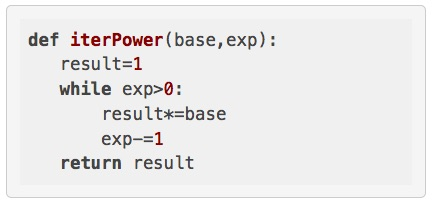
\includegraphics[width=0.5\linewidth]{Body/figures/overcode/largest_stack_cropped.jpg}
\caption{A solution synthesized by OverCode that represents 1538 student solutions.}
\label{largestStack}
\end{figure}

\section{Solution Variation}

In this thesis, {\it solution variation} means three things: correctness, approach, and readability. Since correctness is difficult to prove for an arbitrary piece of code, it is approximated in industry and education by correctness with respect to a set of test cases. In education, the machinery that checks for correctness is often called an autograder.

There is a wide range of solutions that pass all the test cases and are labeled correct by the autograder, but they are not all equally good. Figure~\ref{table:diffapproaches} shows three different solutions of widely varying approach and readability that are correct with respect to the autograder test cases.

\begin{figure}
\begin{tabular}{ll}
{\bf Iterative Solution} & {\bf Recursive Solution} \\
\begin{minipage}{0.5\linewidth}
\begin{lstlisting}[basicstyle=\linespread{1.0}\ttfamily\footnotesize,language=python]
def power(base,exp):
    result=1
    while exp>0:
        result*=base
        exp-=1
    return result
\end{lstlisting}
\end{minipage}
&
\begin{minipage}{0.5\linewidth}
\begin{lstlisting}[basicstyle=\linespread{1.0}\ttfamily\footnotesize,language=python]
def power(base,exp):
    if exp == 0:
        return 1
    else:
        return base * power(base, exp-1)
\end{lstlisting}
\end{minipage} \\
% \end{tabular}

% \begin{tabular}{l}
{\bf Poorly Written Solution} & \\
\begin{minipage}{0.5\linewidth}
\begin{lstlisting}[basicstyle=\linespread{1.0}\ttfamily\footnotesize,language=python]
def power(base, exp):
    tempBase=base
    result = base

    if type(base)==int:
        while exp==0:
            result = 1
            print(result)
            break
        exp=exp-1
        while exp >0:
            tempCal=abs(tempBase)
            exp=exp-1
            while exp<0:
                break
            for i in range (1,tempCal):
                result=result+base
                tempCal=tempCal-1
                tempRes=base
            base=result
        return(result)

    else:
        result = 1
        while exp > 0:
            result = result* base
            exp = exp- 1
        return result
\end{lstlisting}
\end{minipage} 
\end{tabular}
\caption{Three different solutions that exponentiate a base to an exponent. They are all marked correct by the autograder because they pass all the autograder test cases.}
\label{table:diffapproaches}
\end{figure}

Solutions can have different approaches. For example, a student might be subversive and disregard a request by the teacher to solve the problem without using an existing equivalent library function. Or the student might include unnecessary lines of code that reveal possible misconceptions about how the language works. Figure~\ref{table:morediffapproaches} gives an example of each.

\begin{figure}
\begin{tabular}{ll}
{\bf Subversive Solution} &  \\
\begin{minipage}{0.5\linewidth}
\begin{lstlisting}[basicstyle=\linespread{1.0}\ttfamily\footnotesize,language=python]
def power(base, exp):
  return base**exp
\end{lstlisting}
\end{minipage}
& \\
% \end{tabular}

% \begin{tabular}{l}
{\bf Solution with Unnecessary Statement} & \\
\begin{minipage}{1.0\linewidth}
\begin{lstlisting}[basicstyle=\linespread{1.0}\ttfamily\footnotesize,language=python]
def power(base,exp):
 result=1
 while exp>0:
     result=result*base
     exp-=1
     continue #keyword here does not change execution
 return result
\end{lstlisting}
\end{minipage} 
\end{tabular}
\caption{Two different approaches to solving the problem. The first disregards teacher instructions to not use equivalent library functions and the second includes the keyword \texttt{continue} in a place where it is completely unnecessary, casting doubt on student understanding of the keyword \texttt{while}.}
\label{table:morediffapproaches}
\end{figure}

Approaches can be common or uncommon. One can think of the students submitting solutions as a generative function that produces a distribution of solutions we could characterize and take into account while teaching or designing new course material. Figure~\ref{table:commonuncommon} shows the most common and one of the most uncommon solutions produced by students for a problem assigned in 6.00x, an introductory programming course offered on edX in the fall of 2012. Uncommon solutions may be highly innovative or extraordinarily poor.

\begin{figure}
\begin{tabular}{ll}
{\bf Common Solution} & {\bf Uncommon solution} \\
\begin{minipage}{0.5\linewidth}
\begin{lstlisting}[basicstyle=\linespread{1.0}\ttfamily\footnotesize,language=python]
def power(base,exp):
  result=1
  while exp>0:
      result*=base
      exp-=1
  return result
\end{lstlisting}
\end{minipage}
& 
% \end{tabular}

% \begin{tabular}{l}
 % & \\
\begin{minipage}{1.0\linewidth}
\begin{lstlisting}[basicstyle=\linespread{1.0}\ttfamily\footnotesize,language=python]
def power(base,exp):
  if exp == 0:
      return 1
  else:
      return base * power(base, exp-1)
\end{lstlisting}
\end{minipage} 
\end{tabular}
\caption{Common and uncommon solutions to exponentiating a base to an exponent produced by students in the 6.00x introductory Python programming course offered by edX in the Fall of 2012.}
\label{table:commonuncommon}
\end{figure}

Readability is the third critical component of solution variation. Poorly written solutions like the one in Figure~\ref{table:diffapproaches} may be both the symptom and the cause of student confusion. Unreadable code is harder to understand and debug, for both teacher and student. In industry, peer-to-peer code reviews help prevent code with poor readability from entering code bases, where it can be difficult and costly to maintain.

Student design choices affect correctness, approach, and readability. Examples include choosing:
\begin{itemize} 
\item \texttt{for} or ~\texttt{while}
\item \texttt{a *= b} or \texttt{a = a*b}
\item recursive or iteration 
\end{itemize}
Solution variation is a result of these choices. Even simple differences, like comments, statement order, formatting and variable names can make solutions look quite different to the unaided eye, as shown in Figure~\ref{table:difflook}.

\begin{figure}
\begin{tabular}{ll}
% {\bf Solution } & {\bf Uncommon solution} \\
\begin{minipage}{0.5\linewidth}
\begin{lstlisting}[basicstyle=\linespread{1.0}\ttfamily\footnotesize,language=python]
def iterPower(base, exp):
  '''
  base: int or float.
  exp: int >= 0

  returns: int or float, base^exp
  '''
  result = 1
  while exp > 0:
      result *= base
      exp -= 1
  return result
\end{lstlisting}
\end{minipage}
& 
% \end{tabular}

% \begin{tabular}{l}
 % & \\
\begin{minipage}{1.0\linewidth}
\begin{lstlisting}[basicstyle=\linespread{1.0}\ttfamily\footnotesize,language=python]
def iterPower(base, exp):
  wynik = 1

  while exp > 0:
      exp -= 1  #exp argument is counter

      wynik *= base

  return wynik
\end{lstlisting}
\end{minipage} 
\end{tabular}
\caption{These two solutions only differ by comments, statement order, formatting, and variable names. Note: \texttt{wynik} means `result' in Polish.}
\label{table:difflook}
\end{figure}

\section{A Challenge and an Opportunity}

When teachers may have hundreds or thousands of raw student solutions to the same problem, it becomes arduous or impractical to review them by hand. And yet, only testing for approximate correctness via test cases has been automated. Identifying student solution approaches and readability automatically are still open areas of research. Given the volume and variety of student solutions, how do teachers comprehend what their students wrote? How do they give feedback on approach and readability at scale? 

What value can {\it only} be extracted from a massive programming class? This thesis focuses on the opportunity posed by exploiting solution variation within large datasets of student solutions to the same problem. With algorithms, visualizations and interfaces, teachers may learn from their students by exposing student solutions they did not know about before. Teachers could find better examples to pull out for discussion. Teachers could write better feedback, test cases, and evaluation rubrics, given new knowledge of the distribution of student solutions across the dimensions of correctness, approach, and readability. And students could be tapped as experts on the solutions they create and the bugs they fix.

\section{A Tale of Two Turing Machines}

A short story about my time as a teaching assistant illustrates some of the challenges posed by solution variation. Students were programming simulated Turing machines, which compute by reading and writing to a simulated infinitely long tape. I struggled to help a student whose approach was not familiar to me. I could not tell if the approach was fatally flawed or unusual and possibly innovative. I did not want to dissuade him from a novel idea simply because I did not recognize it.

The staff server had thousands of previously submitted correct student solutions, but I could not easily see if one of them successfully employed the same approach as the one envisioned by the struggling student. After experimenting with different representations, I found a visualization of Turing machine behavior on test cases that separated 90\% of the correct student solutions into two main approaches~\cite{ICERGlassman}. The remaining approximately 10\% of solutions included less common strategies. Two solutions passed all test cases but subverted teacher instructions. Many teaching staff members were not aware that there were multiple solutions to the problem and that the current test suite was insufficient to distinguish correct solutions from incorrect ones. At least one staff member admitted steering students away from solutions they did not recognize, but in retrospect may have indeed been valid solutions.

\section{Research Questions}

When a teacher cannot read all the student solutions to a programming problem because there are too many of them,
\begin{itemize}
\item {\bf R1} how can the teacher understand the common and uncommon variation in their student solutions?
\item {\bf R2} how can the teacher give feedback on approach and readability at scale?
\item {\bf R3} ... in a personalized way?
\item {\bf R4} ... and how can students do the same?
\end{itemize}

\subsection{Systems Built}
In this thesis, several systems and workflows are developed and studied to better answer these questions. The first is OverCode, a system for visualizing variation in student Python solutions. The second is Foobaz, a system for visualizing variable name variation and delivering personalized feedback on naming choices. The third and fourth systems are based on two novel, complementary learnersourcing workflows that help students write hints for each other through self-reflection and comparison with other student solutions.

%\subsection{Addressing {\bf R1}, {\bf R2}, and {\bf R3} with OverCode and Foobaz}

\subsubsection{OverCode}

Understanding solution variation is important for providing appropriate feedback to students at scale. In one-on-one scenarios, understanding the space of potential solutions can help teachers counsel students struggling to implement their own solutions. The wide variation among these solutions can be a source of pedagogically valuable examples for course materials and forum posts and expose corner cases that spur autograder refinements.

OverCode, shown in Figure~\ref{fig:fullovercodeinterface} renders thousands of small student Python solutions to the same problem and makes them explorable. With OverCode, teachers can better understand the distribution of common and uncommon solutions without reading every student solution. The OverCode analysis pipeline uses both static and dynamic analysis to normalize and cluster similar solutions into stacks represented by a single normalized solution. The OverCode normalization process and user interface work together to support human readability and switching between solutions with minimal cognitive load. In two user studys, OverCode helped teachers more quickly develop a high-level view of students' understanding and misconceptions and compose feedback that is relevant to more student solutions, compared to the status quo.

A key, novel component of the normalization process is identifying {\it common variables} across multiple student solutions to the same programming problem. Common variables are found in multiple student solutions to the same problem and have identical sequences of distinct values when those solutions are executed on the same test cases. During normalization, every common variable in every solution is renamed to the most popular name students gave it. 

The normalized solutions encode both static and dynamic information. More specifically, its syntax carries the static information and its variable names encode dynamic information. A single normalized solution can represent an entire stack of hundreds or thousands of similar student solutions.

\begin{figure}
\centering
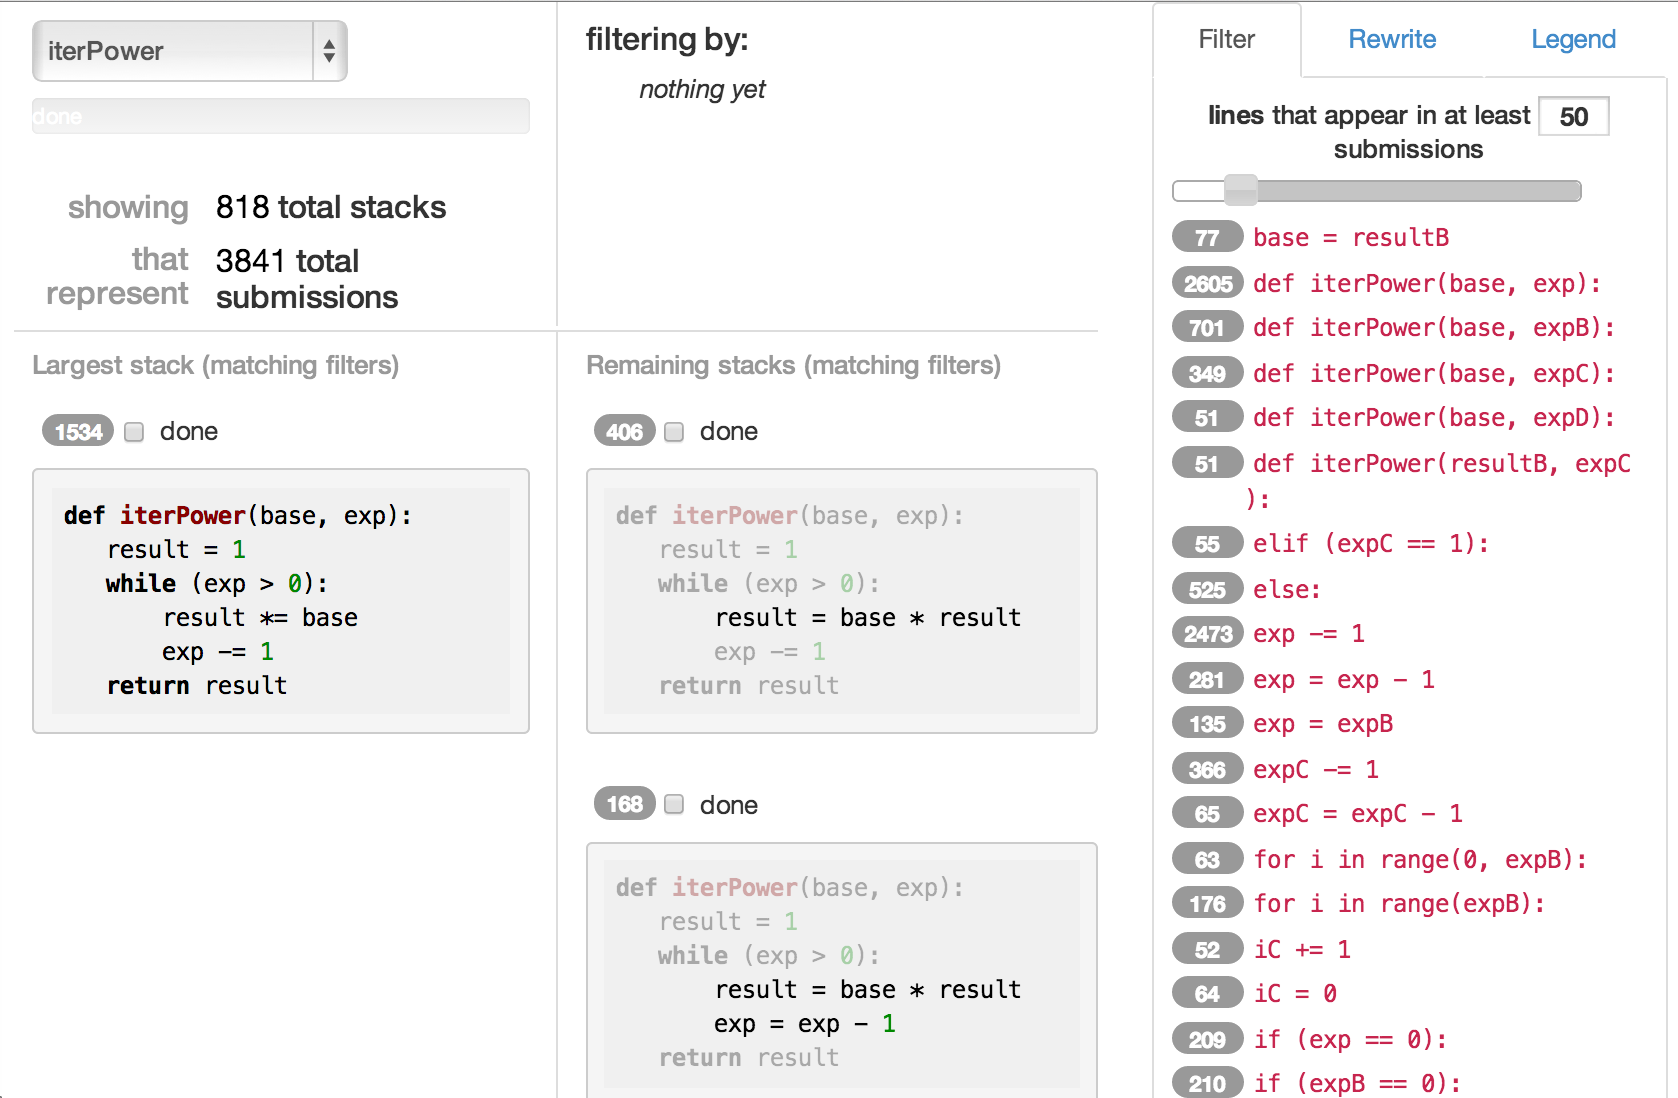
\includegraphics[width=1.0\linewidth]{Body/figures/interfaceScreenShot.png}
\caption{The OverCode user interface. The top left panel shows the number of clusters, called {\it stacks}, and the total number of solutions visualized. The next panel down in the first column shows the largest stack, while the second column shows the remaining stacks. The third column shows the lines of code occurring in the normalized solutions of the stacks together with their frequencies.}
\label{fig:fullovercodeinterface}
\end{figure}

\subsubsection{Foobaz}

Traditional feedback methods, such as hand-grading student solutions for approach and readability, are labor intensive and do not scale. Foobaz transforms the output of the OverCode analysis pipeline into an interface for teachers to compose feedback at scale on a critical aspect of readability, variable naming. As shown in Figure \ref{fig:foobaz_teacherview}, the Foobaz teacher interface displays the most common and uncommon names for variables in each stack of solutions and allows teachers to label good examples of good and bad student-chosen variable names. Students receive these labels in the form of a personalized active learning exercise, where they can learn from the good and bad variable name choices of fellow students. 

Once created, these exercises are reusable for as long as the programming problem specification is unchanged. In the first of two user studies, teachers quickly created exercises that could be personalized to the majority of student solutions collected from a Python programming MOOC. In the second of two user studies, fresh students wrote solutions to the same programming problems and received personalized feedback from the teachers in the previous study. A snapshot of this feedback, in the form of an active learning exercise, is shown in Figure~\ref{fig:foobaz_studentview}. Foobaz demonstrates that teachers can efficiently give feedback at scale on variable naming, a critical aspect of readability.

\begin{figure*}[p]

\begin{subfigure}[b]{1.0\textwidth}
\centering
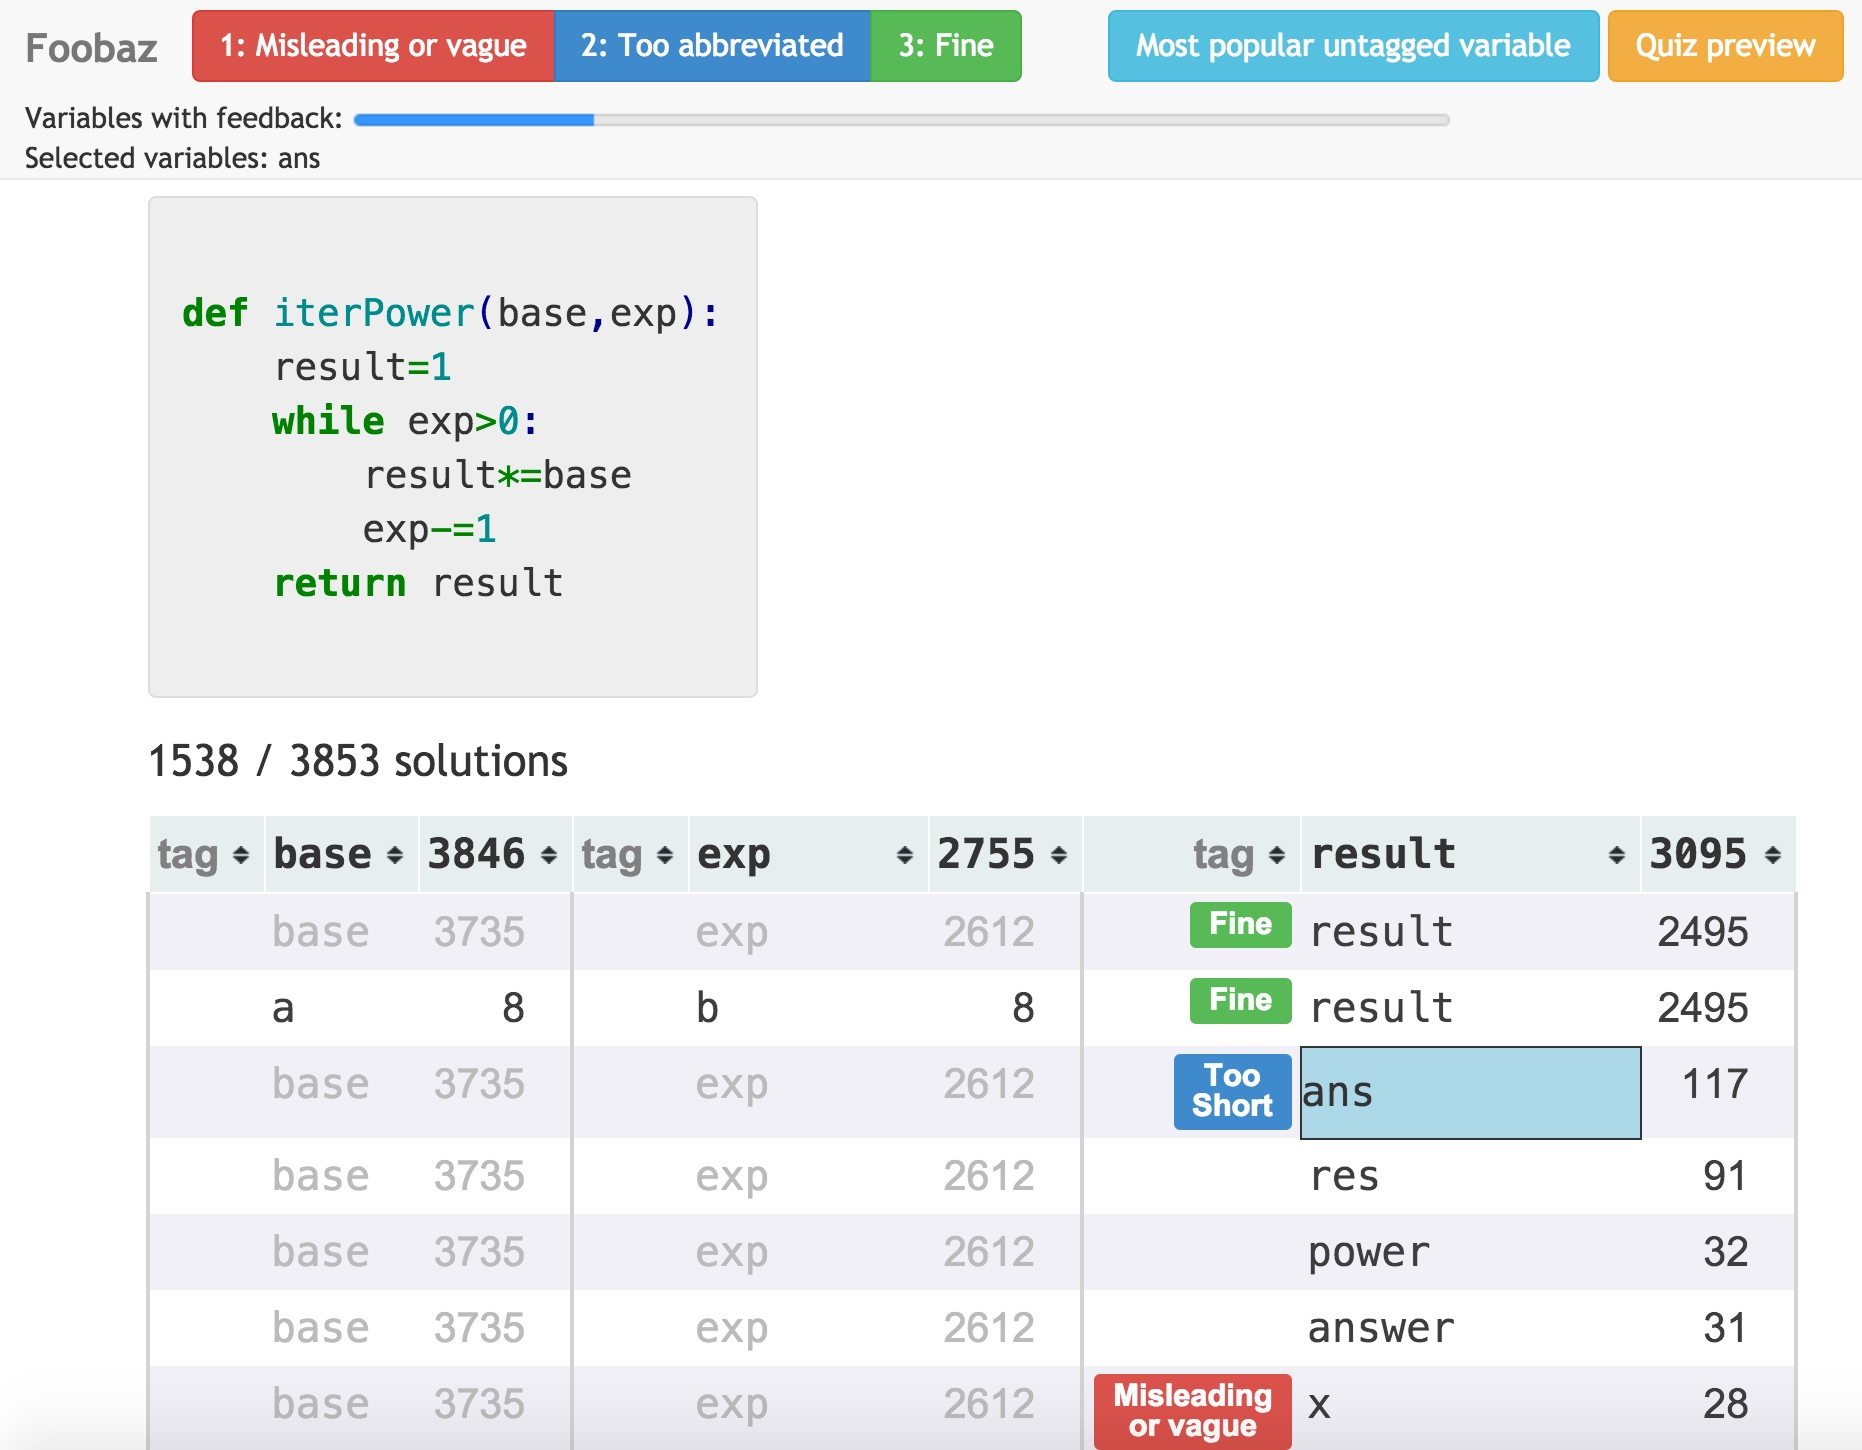
\includegraphics[width=0.75\linewidth]{Body/figures/foobaz/FoobazInitialView4.jpg}
\caption{The Foobaz teacher interface. The teacher is presented with a scrollable list of normalized solutions, each followed by a table of student-chosen variable names. Some names shown here have been labeled by the teacher as ``misleading or vague,'' ``too short,'' or ``fine.''}
\label{fig:foobaz_teacherview}
\end{subfigure}

\begin{subfigure}[b]{1.0\textwidth}
\centering
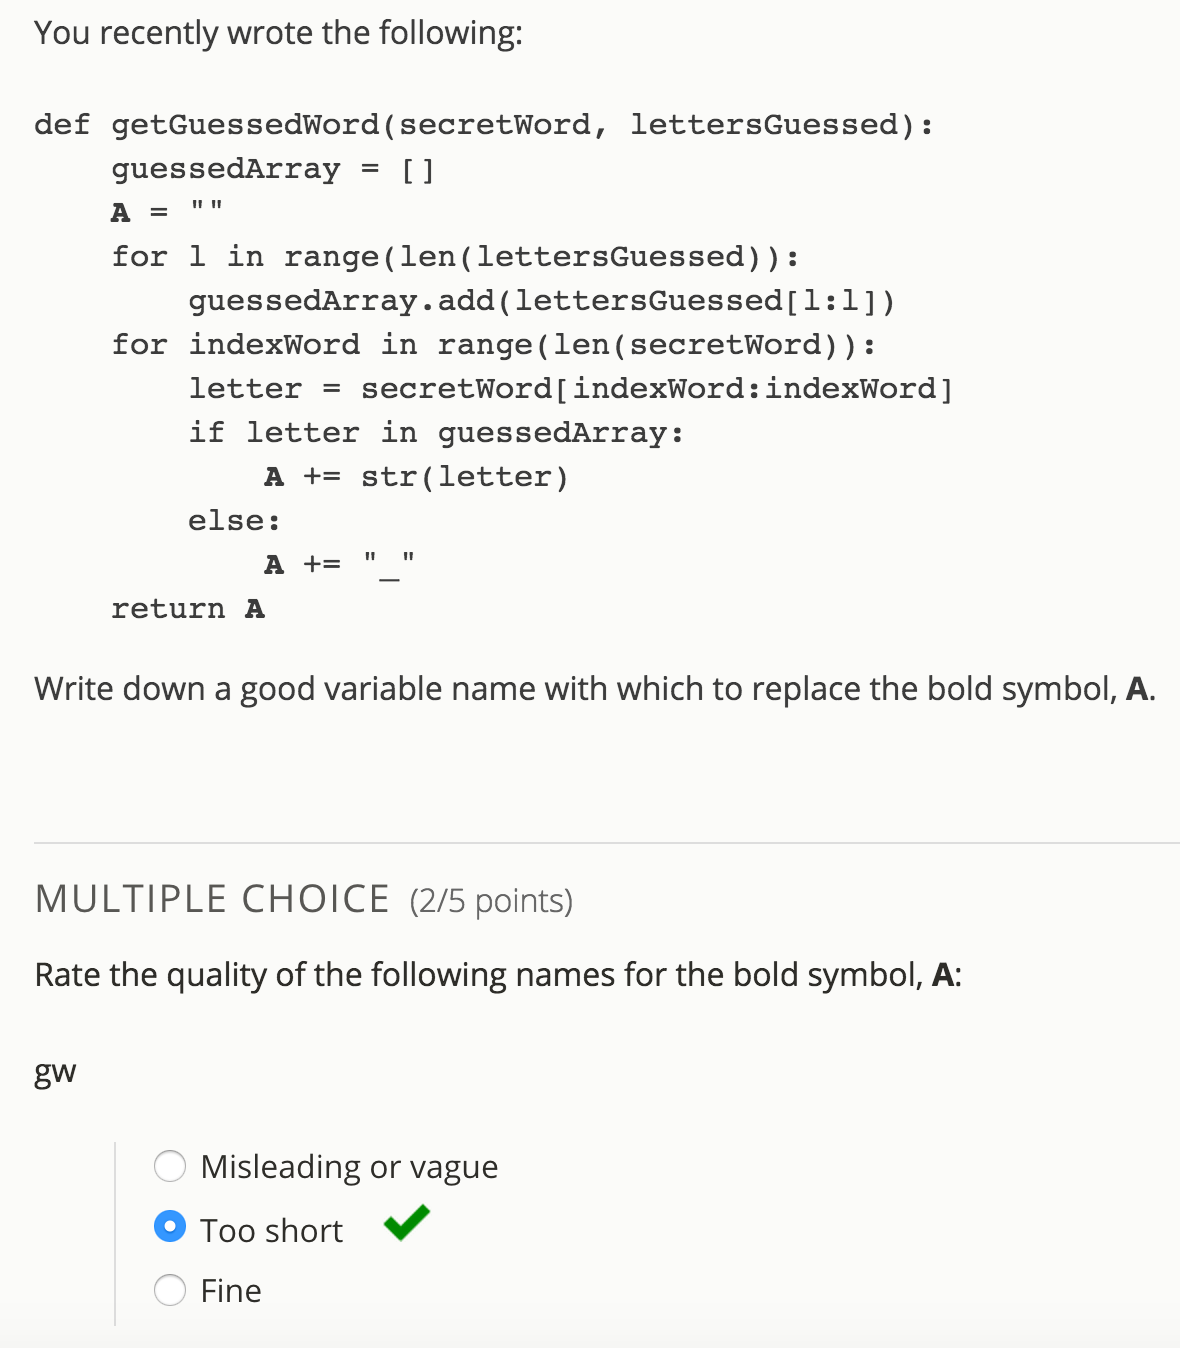
\includegraphics[width=0.4\linewidth]{Body/figures/foobaz/feedbackQuizExample.png}
\caption{A personalized active learning activity as seen by the student, delivered by edX infrastructure. Students are shown their own solution, with a variable name replaced by an arbitrary symbol, followed by variable names for the student to consider and label using the same labels that were available to the teacher. After the student has submitted their own judgments, the teacher labels are revealed, along with teacher comments.}
\label{fig:foobaz_studentview}
\end{subfigure}

\caption{Snapshots of the Foobaz teacher interface and personalized feedback for a student about variable names.}
\end{figure*}

\subsubsection{Learnersourcing Personalized Hints}

Personalization, in the form of one-on-one tutoring, has been a gold standard in educational psychology for decades~\cite{bloom}. It can be hard to get personalized help in large classes, especially when there are many varied solutions and bugs. Students who struggle, then succeed, become experts on writing particular solutions and fixing particular bugs. This thesis describes two workflows built on that insight, shown in Figure~\ref{fig:betagammaworkflow}. 

Unlike prior incarnations of assigning tasks to and collecting data from students, i.e., learnersourcing~\cite{kim2013learnersourcing}, these workflows collect and distribute hints written only by students who earned the expertise necessary to write them. Both workflows give students an opportunity to reflect on their own technical successes and mistakes, which is helpful for learning~\cite{dewey1933} and currently lacking in the engineering education status quo~\cite{asee}. One of the two workflows also systematically exposes students to some of the variation present in other student solutions, as recommended by theories from educational psychology, specifically variation theory~\cite{marton1997learning} and analogical learning theory~\cite{kurtz01learning,loewenstein2003analogical}.

These workflows were applied to programming problems in an undergraduate digital hardware design class with hundreds of students. Field deployments and an in-lab study show that students can create helpful hints for their peers that augment or even replace teachers’ personalized assistance. %, especially when that assistance is not available.


\begin{figure}
\centering
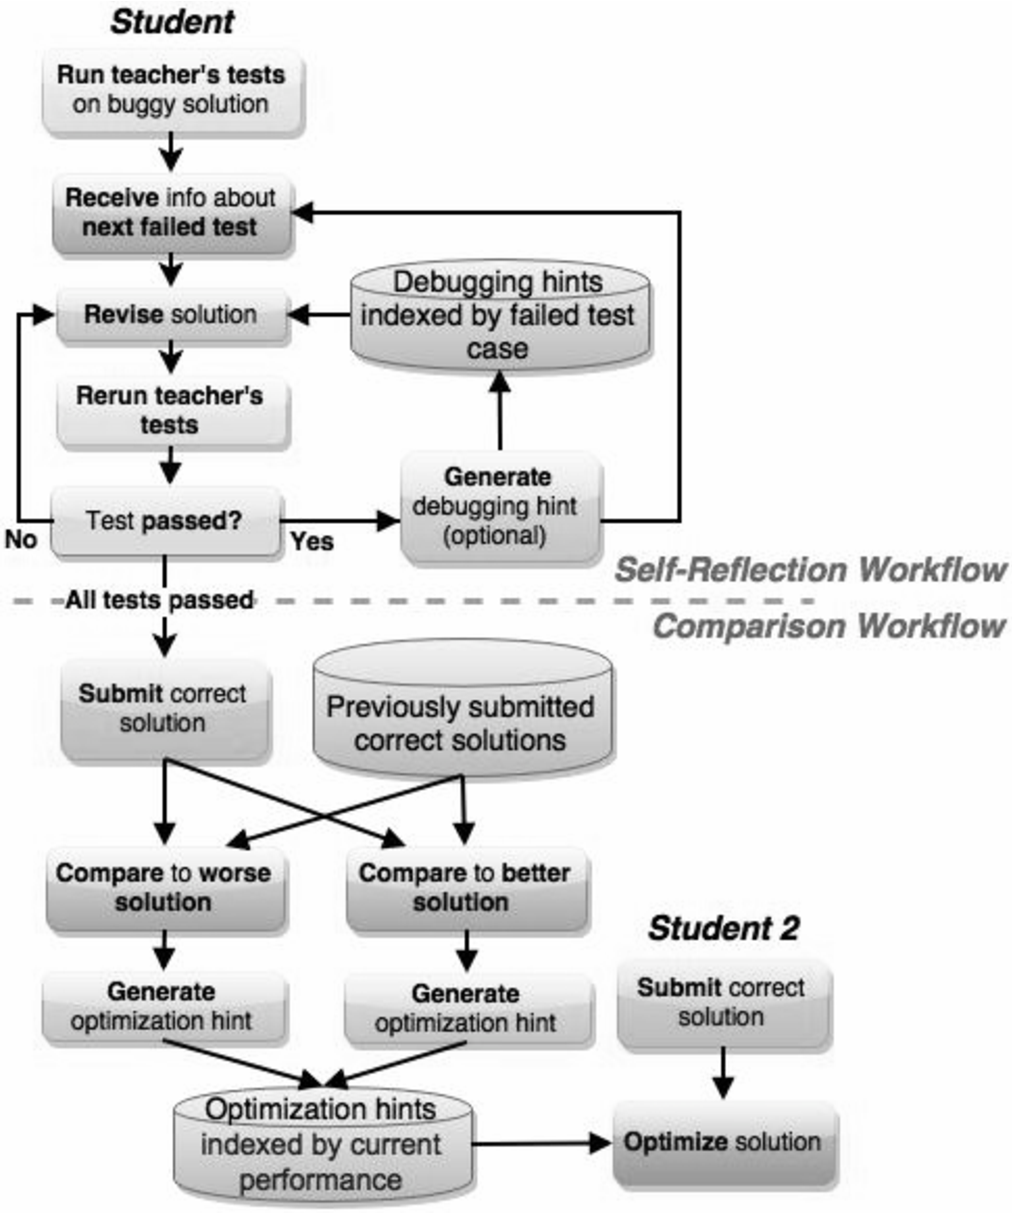
\includegraphics[width=1.0\linewidth]{Body/figures/classoverflow/CombinedWorkflow_grey.pdf}
\caption{In the \textit{self-reflection} workflow, students generate hints by reflecting on an obstacle they themselves have recently overcome. In the \textit{comparison} workflow, students compare their own solutions to those of other students, generating a hint as a byproduct of explaining how one might get from one solution to the other.}
\label{fig:betagammaworkflow}
\end{figure}

\subsection{Systems as Answers to Research Questions}

\subsubsection{{\bf R1} Understanding Variation at Scale}
The OverCode and Foobaz systems both give teachers a better understanding of student solutions and how they vary in approach and readability. OverCode allows teachers to more quickly develop a high-level view of student understanding and misconceptions. Foobaz displays the variety of common and uncommon variable names in student solutions to a single programming problem, so teachers can better understand student naming practices. The clustering and visualization techniques created for both these systems provide some new answers to the research question {\bf R1} for introductory Python problems. 

\subsubsection{{\bf R2} Feedback on Approach and Readability at Scale}
OverCode is also an answer to the research question {\bf R2}. With OverCode, teachers produced feedback on solution approaches that was relevant to more student solutions, compared to feedback informed by status quo tools. 

\subsubsection{{\bf R3} Personalized Feedback on Approach and Readability at Scale}
To create Foobaz, the challenge of delivering personalized feedback on approach and readability at scale was narrowed down to just one critical aspect of readability: variable names. In a one-on-one scenario, a teacher helping a student might notice that the student is choosing poor variable names. The teacher might start a conversation about both their good and bad variable naming choices. In a massive classroom where that kind of chat is not possible, Foobaz delivers personalized active learning exercises intended to spark the same thought processes in the student. Foobaz helps answer {\bf R3} by demonstrating how teachers can compose automatically personalized feedback on an aspect of readability to students at scale. %These exercises are called {\it variable name quizzes}. 

\subsubsection{{\bf R4} Personalized Feedback at Scale}
The two novel workflows that collect and deliver personalized student-written hints address this final research question in a general way. Their instantiations as systems deployed in an undergraduate engineering course demonstrated that, given appropriate design choices and prompts, students can give personalized feedback in large-scale courses.



\begin{comment}It can be hard to get personalized help in large-scale programming classes, especially when there are many different possible solutions and bugs. Personalized support is a gold standard in education, but it scales poorly with the number of students. The key insight in this thesis is that students who struggle and then succeed become experts on the particular solutions they wrote and bugs they fixed. The students can then write hints for fellow and future students based on their new expertise. This thesis presents two complementary workflows for helping students help each other in ways that are also beneficial to themselves, according to learning science theories like variation theory and analogical learning.

Prior work on {\it learnersourcing}~\cite{kim2013learnersourcing} prompted students to perform tasks, like summarizing a portion of a video lesson, that would help them and fellow learners. Unlike general learnersourcing,  targeted form of learnersourcing allows or prompts specific students to help current or future students on challenges they have already conquered. In the process of participating in the workflows, students engage in self-reflection, self-explanation, and comparison with alternatives, hopefully within their zone of proximal development. The literature described in the chapter on Related Work suggests that these activities promote learning. Both workflows were evaluated in an undergraduate digital circuit design class with hundreds of students. Within these targeted learnersourcing workflows, students can create helpful hints for their peers that augment or even replace teachers' personalized assistance, especially when that assistance is not available. 



The learnersourcing workflows in this thesis are more targeted. Hint writers or receivers are not drawn from the pool of all students who worked on the problem, they are prompted to write hints for 

 can be prompted to write a hint about how to solve the problem well because they wrote a particular type of solution to the problem and have earned the expertise to help


 another student who wrote a solution like theirs or even slightly worse than theirs. They can be selected to receive a hint because another student has Or they can be selected to receive a hint they are failing particular test case(s).


Two  uses new workflows to harvest and organize students’ collective knowledge and advice for helping fellow novices through design problems in engineering (see Fig- ure 5-1). ClassOverflow was evaluated in an undergraduate digital hardware design class with hundreds of students. We show that, given our design choices, students can create helpful hints for their peers that augment or even replace teachers’ personalized assistance, especially when that assistance is not available.

Rather than depend on teachers, this thesis presents two workflows that enable students with earned expertise about a particular solution or bug to write hints for students who need

Rather than depend on teachers, fellow students who have already written a solution 

When the space of possible solutions and bugs is large, fellow  personalized support may be 

 {\it Learnersourcing}~\cite{kim2013learnersourcing} addresses this

Students can collectively write many different solutions of varying quality for the same problem

, and the space of possible bugs accumulated over all paths to each solution can be very large. Teachers can model good debugging strategies and give qualitative feedback on student solutions they never implemented themselves have not themselves already created, but students, through their own experience struggling with a particular problem, can become experts on the particular optimizations they implement or bugs they resolve.
\end{comment}




\section{Thesis Statement and Contributions}

The systems described in this thesis show various mechanisms for handling and taking advantage of solution variation in massive programming courses. Students produce many variations of solutions to a problem, running into common and uncommon bugs along the way. Students can be pure producers whose solutions are analyzed and displayed to teachers. Alternatively, students can be prompted to generate analysis of their own and others' solutions, for the benefit of themselves and current and future students. %, and sends it to selected fellow learners as feedback. %We would like to demo these systems together, as a suite of learnersourcing systems that allow teachers to turn the challenges of teaching at scale into an opportunity for discussion, self-reflection, peer-teaching, and more learning from examples.

My thesis statement is: 
\begin{displayquote}
Clustering and visualizing solution variation collected from programming courses can help teachers gain insights into student design choices, detect autograder failures, award partial credit, use targeted learnersourcing to collect hints for other students, and give personalized style feedback at scale.
\end{displayquote}

The main contributions of this thesis are:
\begin{itemize}
\item An algorithm that uses the behavior of variables to help cluster Python solutions and generate the platonic solution for each cluster. Platonic solutions are readable and encode both static and dynamic information, i.e., the syntax carries the static information and the variable name encodes dynamic information.
\item A novel visualization that highlights similarity and variation among thousands of Python solutions while displaying platonic solutions for each variant. 
\item Two user studies that show this visualization is useful for giving teachers a bird's-eye view of thousands of students' Python solutions.
\item A grading interface that shows similarity and variation among Python solutions, with faceted browsing so teachers can filter solutions by error signature, i.e., the test cases they pass and fail. 
\item Two field deployments of the grading interface within introductory Python programming exam grading sessions.
\item A technique for displaying clusters of Python solutions with only an aspect, i.e., variable names and roles, of each cluster exposed, revealing the details that are relevant to the task. %In this application, the relevant features are variable names and roles.
\item A workflow for generating personalized active learning exercises, emulating how a teacher might socratically discuss good and bad choices with a student while they review the student's solution together. 
\item An implementation of the above technique and method for variable naming. % within datasets from both MOOCs and large residential classes on introductory Python programming.
\item Two lab studies which evaluate both the teacher and student experience of the workflow applied to variable names.
\item A self-reflection learnersourcing workflow in which students generate hints for each other by reflecting on an obstacle they themselves have recently overcome while debugging their solution.
\item A comparison learnersourcing workflow in which students generate design hints for each other by comparing their own solutions to alternative designs submitted by other students.
\item Deployments of both workflows in a 200-student digital circuit programming class, and an in-depth lab study with 9 participants.
\end{itemize}

\section{Thesis Overview}

Chapter \ref{chapter:relatedwork} summarizes prior and contemporary relevant research on systems that support programming education. It also briefly explains theories from the learning sciences and psychology literature that influenced or support the pedagogical value of the design choices made within this thesis.

The four chapters that follow describe, in detail, the four systems developed, as well as their evaluation on archived data or in the field.

\begin{itemize}
\item OverCode (Chapter \ref{chapter:overcode}) visualizes thousands of programming solutions using static and dynamic analysis to cluster similar solutions. It lets teachers quickly develop a high-level view of student understanding and misconceptions and provide feedback that is relevant to many student solutions. It also describes GroverCode, an extension of OverCode optimized for grading correct and incorrect student solutions.

\item Foobaz (Chapter \ref{chapter:foobaz}) clusters variables in student solutions by their names and behavior so that teachers can give feedback on variable naming. Rather than requiring the teacher to comment on thousands of students individually, Foobaz generates personalized quizzes that help students evaluate their own names by comparing them with good and bad names from other students. 

\item Chapter \ref{chapter:classoverflow} describes two workflows that collect and organize solution hints indexed by (1) the autograder test that failed or (2) a performance characteristic like size or speed. It helps students reflect on their debugging or optimization process, generates hints that can help other students with the same problem, and could potentially bootstrap an intelligent tutor tailored to the problem.

\item Chapter \ref{chapter:grovercode} describes Bayesian clustering and mixture modeling algorithms applied to the OverCode pipeline output for extracting additional insight into patterns within student solutions. 
\end{itemize}

Chapter \ref{chapter:discussion} discusses some of the insights that came out of building and testing the systems in this thesis. Chapter \ref{chapter:conclusion} outlines avenues of future work on the systems and ideas in this thesis, in combination with the complementary work of others in this space.
%%% This is an example first chapter.  You should put chapter/appendix that you
%% write into a separate file, and add a line \include{yourfilename} to
%% main.tex, where `yourfilename.tex' is the name of the chapter/appendix file.
%% You can process specific files by typing their names in at the 
%% \files=
%% prompt when you run the file main.tex through LaTeX.
\chapter{Related Work}\label{chapter:relatedwork}

Systems that help students in massive programming courses may build on work from any or all the following related fields: program analysis, program synthesis, crowd workflows, user-interface design, machine learning, and learning science. First, I present prior work and theories of how people learn that later inspired key design decisions. I then clarify how this thesis work is novel by describing related work that achieves similar goals or uses similar methods.

Computers' potential as teaching aids was recognized soon after their development; not long after it was physically possible to bring a computer into the classroom, they were used as vehicles for education \cite{computersInEdu}. Modern computer-aided instruction includes intelligent tutoring systems, automated tutorials, power-grading systems, and massive open online course platforms. 

\todo{add cody! (see ICER submission)}
\todo{look into PHOG and other interesting work here: http://www.srl.inf.ethz.ch/spas.php http://www.srl.inf.ethz.ch/raychev.php and "Predicting Program Properties from “Big Code” http://www.srl.inf.ethz.ch/papers/jsnice15.pdf and "Code Completion with Statistical Language Models" http://www.srl.inf.ethz.ch/papers/pldi14-statistical.pdf}

\todo{Analyzing Engineering Design through the Lens of Computation
Authors
Marcelo Worsley, Paulo Blikstein}

\todo{Teaching composition quality at scale: human judgment in the age of autograders
Authors
John DeNero, Stephen Martinis}

\todo{Problems Before Solutions: Automated Problem Clarification at Scale
Authors
Soumya Basu, Albert Wu, Brian Hou, John DeNero}

\todo{CS10K Teachers by 2017?: Try CS1K+ students NOW! Coping with the Largest CS1 Courses in History
Authors
Daniel D Garcia, Jennifer Campbell, John DeNero, Mary Lou Dorf, Stuart Reges}

\todo{Fuzz Testing Projects in Massive Courses
Authors
Sumukh Sridhara, Brian Hou, Jeffrey Lu, John DeNero}

\todo{https://computinged.wordpress.com/2012/12/14/research-questions-on-moocs-whos-talking-whos-completing-and-wheres-the-teaching/}

\todo{https://computinged.wordpress.com/2012/08/14/daphne-kollers-ted-talk-whats-new-about-moocs/

The Relative Effectiveness of Human Tutoring,
Intelligent Tutoring Systems, and Other Tutoring
Systems
KURT VanLEHN $http://www.public.asu.edu/~kvanlehn/Stringent/PDF/EffectivenessOfTutoring_Vanlehn.pdf$}

\todo{cite Techniques for Plan Recognition
SANDRA CARBERRY for solution path mining, but I did not do that...}
\todo{Automated Feedback Generation for

Introductory Programming Assignments

Rishabh Singh}

\todo{Learning Design Patterns
with Bayesian Grammar Induction
Jerry O. Talton et al. http://graphics.stanford.edu/~lfyg/gi.pdf}

\todo{http://cs.stanford.edu/people/sharmar/pubs/ddec.pdf Data-driven equivalence checking}

\todo{Mining Source Code Repositories at Massive Scale
using Language Modeling
Miltiadis Allamanis, Charles Sutton}

\todo{Student coding styles as predictors of help-seeking behavior
Authors
Engin Bumbacher, Alfredo Sandes, Amit Deutsch, Paulo Blikstein}

\todo{see library on Google Scholar, Vineet's review of literature}

\todo{Programming Pathways: A Technique for Analyzing Novice Programmers’ Learning Trajectories
Authors
Marcelo Worsley, Paulo Blikstein}

\todo{Educational data mining and learning analytics: Applications to constructionist research
Authors
Matthew Berland, Ryan S Baker, Paulo Blikstein}

\todo{cite WebZeitGeist}

\todo{Programming pluralism: Using learning analytics to detect patterns in the learning of computer programming
Authors
Paulo Blikstein, Marcelo Worsley, Chris Piech, Mehran Sahami, Steven Cooper, Daphne Koller}

\todo{cite Using learning analytics to assess students' behavior in open-ended programming tasks
Authors
Paulo Blikstein}

\todo{Modeling how students learn to program
Authors
Chris Piech, Mehran Sahami, Daphne Koller, Steve Cooper, Paulo Blikstein}

\todo{see Related Work folder in Google Drive and Question Independent Grading using Machine Learning:

The Case of Computer Program Grading

Gursimran Singh

Shashank Srikant

Varun Aggarwal}

\todo{add The Sweep: Essential Examples for In-Flow Peer Review by
JG Politz, JM Collard, A Guha, K Fisler, S Krishnamurthi and In-flow peer-review of tests in test-first programming
Authors
Joe Gibbs Politz, Shriram Krishnamurthi, Kathi Fisler and In-Flow Peer Review
Authors
Dave Clarke, Tony Clear, Kathi Fisler, Matthias Hauswirth, Shriram Krishnamurthi, Joe Gibbs Politz, Ville Tirronen, Tobias Wrigstad and CaptainTeach: a platform for in-flow peer review of programming assignments
Authors
Joe Gibbs Politz, Shriram Krishnamurthi, Kathi Fisler and CaptainTeach: Multi-stage, in-flow peer review for programming assignments
Authors
Joe Gibbs Politz, Daniel Patterson, Shriram Krishnamurthi, Kathi Fisler}

\todo{add this to related work https://computinged.wordpress.com/2016/05/16/implementing-design-studio-pedagogy-with-an-augmented-reality-cs-classroom/}

\section{Learning from Variation}

\begin{comment}
Marton et al.'s variation theory \cite{Marton13} holds that in order to learn something, one must see examples that vary along particular dimensions: ``contrast,'' as in pairing it with something it is not; ``generalization,'' as in presenting multiple instances of the object or concept to be learned, varying only that which is irrelevant; ``separation,'' as in presenting multiple instances of the object or concept, varying only that which can vary internally without changing the object or concept into something else; and ``fusion,'' as in seeing multiple examples in which previously analytically separated aspects must be processed together to recognize the object or concept. The aspects which are related to these dimensions of variation and therefore define the object or concept are called ``critical features.''
\end{comment}

\subsection{Variation Theory}
Marton's Variation Theory, as summarized by Suhonen et al. \cite{suhonen}, is defined by the dimensions of variation necessary to fully communicate a concept to a student: \emph{contrast} (``in order to experience something, a person must experience something else to compare it with''); \emph{generalization}, or the ways something can vary without becoming something else; \emph{separation}, or looking at the variation only across specific features; and \emph{fusion}, where multiple critical aspects of the concept are varied simultaneously. In other words, variation reveals which aspects of a phenomenon are superficial/irrelevant and which are innate/critical to its definition \cite{Leung}. These aspects that define the object or concept are called ``critical features.'' The Variation Theory is a framework that now guides the design of some critical reading exercises \cite{Tong} and exercises for novice programmers \cite{eckerdal}. 

Given Marton et al.'s rubric for effective patterns of variation, and the identification of ``critical features,'' one can discern between more or less theoretically effective examples of the object or concept given to a student to learn. On this basis, Luxton-Reilly et al. \cite{Luxton13} suggest that identifying distinct clusters of solutions can help instructors select appropriate examples of code for helping students learn. They also suggest that it is helpful for teachers' own understanding and quality of feedback and guidance. Facilitating the discovery or identification of critical features, which are possibly both teacher-specific and task-specific, is a major challenge I will address in this thesis. 

Other pedagogical strategies that involve comparing and contrasting examples have also been shown to have learning benefits. The pedagogical method of comparing and contrasting ways of approaching a solution has now been validated in the literature of mathematics education research \cite{Star07}, cognitive science \cite{loewenstein2003analogical,kurtz01learning,telling}, and computing education research \cite{Suhonen08, PatitsasICER13}. Peer reviews and assessments, surveyed in \cite{peerReview98}, are yet another opportunity for students to learn from compare and contrast.

\subsection{Synthesizing Knowledge Across Sources and Modalities}

The synthesis of understanding derived from multiple sources is critical to journalism and humanities scholarship and in technical fields, like mathematics.

\subsubsection{Humanities Scholarship and Journalistic Analysis}  
Wineburg \cite{wineburg} shows how students of history come to their understanding of complex events. One important behavior is the students' use of multiple simultaneous documents to understand context. Wineburg finds that ``\ldots context is everything \ldots who wrote something; what their political view is; what the situation in the world is at that moment \ldots you need to see the situation from many points-of-view \ldots''

Software has recently been built to help scholars and journalists analyze and synthesize knowledge across sources. For example, the AP's Overview Project is an example of software designed to help journalists analyze thousands of documents. Similarly, WordSeer \cite{wordseer} allows scholars in the humanities to make sense of a corpus of relevant texts by providing the ability to look at multiple sources and do textual analysis of the content. Crowdlines \cite{luther} employed crowd-sourcing to help people learn and synthesize information from diverse online sources. Since humans are skilled at evaluating high-level structure and making connections between sources, crowdworkers created outlines for important topics that included diverse perspectives from multiple document sources. 

Shahaf et al. \cite{shahaf} created algorithms for ``information cartography,'' algorithmically sub-sampling large collections of documents on a common topic and laying them out as a 2-D map of interrelated documents for users to explore and read. This technique has been applied to scholarly publications and news articles on complex current events, such as the European debt crisis or the Israeli-Palestinian conflict. These domains contain interrelated parallel story-lines that evolve and intersect over time, and are represented as such in the resulting ‘Metro Maps’ of information.

\subsubsection{Science, Technology, Engineering and Math (STEM)} 
The simple question, ``What machine learning books are accessible and appropriate for my high school-aged daughter?'' recently kicked off a very lively discussion on a corporate engineering mailing list. It is a question that humans with a model of the learner, e.g., high school student, and the subject matter, e.g., machine learning, can answer well. Jardine \cite{jardine} generated reading lists specifically for novices hoping to become experts in a particular area, using a personalized pagerank function and Latent Topic Models. 

Educational psychologists have found that multiple explanations within and across multiple modalities can help students learn mathematical problem solving. Both Tabachneck et al. \cite{Tabachneck} and Cox and Brna \cite{cox} found that students fared better at problem solving when using multiple strategies and/or representations, such as diagrams, written algebra, tables, and natural language. Ainsworth points out that giving students an opportunity to consider different representations may help them overcome the weaknesses of any particular representation.

This is also supported by authors of Metacademy.com, a popular online resource for teaching yourself machine learning: ``A good general piece of advice is to consult multiple resources. Different textbooks or courses will explain something from a different perspective \ldots [O]ften when reading one, you get an ‘aha!’ moment for something which didn't make sense in the other. Unfortunately, this option might not be practical unless you have access to a university library.'' \cite{metacademy}

\subsection{User Interface Design}
Tufte pioneered a layout technique called ``small multiples,'' designed to help viewers make rapid decisions about a wide array of items or variables: ``Small multiple designs \ldots answer directly by visually enforcing \ldots the differences among objects, \ldots the scope of alternatives.'' %We took inspiration from both of these layouts when designing the flowing grid layout for DocMatrix. 

%The common term sidebar was inspired by Hearst's faceted browsing \cite{facets}. But rather than display facets derived from metadata about each document, we extracted the common terms from a source closer to the content of the documents themselves: the tables of contents. Clicking on any of the terms in this list exposes the tables of contents, with relevant chapter titles highlighted; the actual terms contained in the tables of contents are the key to this ontological alignment.

Grokker is a document-clustering visualization system, with small popup windows to read texts in parallel \cite{slaney}. Unlike DocMatrix, Grokker's primary representation of a corpus of documents is as clusters of dots, but the study design and results are still relevant here. The task for Grokker readers was to quickly browse a large document collection, and then answer a set of questions to test their understanding. A key finding of this study was that small details of document viewability and the amount of time it took the participants to access content dramatically affected how much they understood about the domain.  In other words, small changes in the amount of time to switch between related documents was an important variable.  


\section{Methods for Analyzing Solutions}

While the methods described in this section all analyze solutions written in code, either as individuals or as a collection, some focus on supervised classification of solutions using pre-defined schemas and some focus on unsupervised clustering of code within collections; and some focus on explicitly identifying variation.

\subsection{Methods for Supervised Classification of Solutions}

Taherkhani and collaborators have developed several algorithm recognition methods. Two methods feature prominently in their work: (1) a method that creates a feature vector for the \emph{predefined target solution} based on roles of variables, beacons, and various other software metrics and (2) a method that scans solutions for \emph{predefined schemas} that are associated with algorithms of interest. In \cite{taherkhani13}, Taherkhani et al. have combined the two approaches into a more robust version which only compares software metrics and beacons on the code that have the same schema. While the software metrics used in these approaches are relevant to my thesis, the use of predefined schemas and target solutions is distinct from my approach of purely mining student solutions.

\subsection{Methods for Unsupervised Clustering of Code}

Unsupervised clustering encompasses everything from identifying plagiarism within a collection of solutions submitted by different people to loosely grouping solutions with similar approaches to solving a problem.

\subsubsection{Clone Detection}
There are multiple types of clones. The simplest clone is an exact copy. A parameter-substituted clone only differs from its copy by the values of identifiers and literals. A structure-substituted clone is a copy with something new swapped in for an entire subtree of the syntax tree. This is of particular interest to teachers looking for evidence of plagiarism within or across class offerings and for software engineers performing re-factoring who want to make their code more compliant with the DRY ("Do Not Repeat Yourself") principle of software development.

\citet{tiarks2011extended} does... \todo{expand on what I said earlier: The most powerful algorithm recognition methods can identify clones that are modified beyond just structural substitutions...}

A popular plaigerism detection algorithm, MOSS, uses \todo{winnowed?} document fingerprinting by \citet{schleimer2003winnowing}. A fingerprint is constructed by computing hashes for all $n$-grams in a document (for some chosen $n$). Similar code will contain similar fingerprint components. \todo{it also does parameter substitution, right? and what's this winnowing business? did document fingerprinting exist before this citation?}

%These latter two types of clones are difficult to identify even with current state-of-the-art techniques \cite{taherkhani12, taherkhani13}. 

\subsection{Methods for Describing Solution Variation}

\begin{comment}
Braun and Clarke \cite{thematic06} argue that its application to qualitative data outside psychological research is justified. It is in direct contrast to methods in which a hypothesis or theory is first declared, and then evidence for and against it is gathered from the data. 
\end{comment}

\citet{Luxton13} used thematic analysis to capture the variation between correct solutions in their dataset. Thematic analysis comes out of the field of psychology as a way to build theory from observing patterns in organic, free-form statements from subjects, or, in this case, submissions for coding assignments. They aimed to discover the kinds and degree of variation between student-generated solutions that fulfilled the specifications of short introductory Java programming exercises. By thematic analysis of student submissions, the authors generated a taxonomy that captured the variation between correct solutions in their dataset. They then created an Eclipse plug-in for classifying new code examples based on their taxonomy. 

\section{Methods for Analyzing Paths to Solutions}

Using automated classification methods, \citet{Piech} found distinct development paths students take to achieve working solutions that fulfilled the specifications of short introductory programming exercises in Java. Students' incremental paths were classified by pipeline that included milestone discovery, Hidden Markov Modeling of the students' process, and clustering of solution paths. These identified paths are visualized as finite state machine transition diagrams. The evaluation focused on predicting midterm exam grades and detecting milestone difficulty.

\citet{sudol12} also classify and map out distinct paths to solutions to introductory programming exercises. After using a Markov Model to generate a ``problem state graph,'' the authors applied their Probabilistic Distance to Solution (PDS) metric to the graph to estimate the number of states between an observed program model and the model of a correct solution.

Kiesmueller et al. \cite{Kiesmueller} attempted to recognize strategies at a very high level, which are not specific to the challenge at hand. Example high-level problem-independent strategies were a top-down or bottom-up programming style. Helminen et al. \cite{ICERHelminen} introduced novel interactive graphs for examining the problem solving process of students working on small programming-like problems. However, problems with multiple solutions were outside the scope of their investigation.

%\section{Introduction}
\section{Thesis Proposal}

%I partitioned the related work based on method of discovering the space of solutions and existing structures within learning environments that this knowledge could enhance. The specific domain to which these methods and interventions are applied is noted as each reference is discussed. 

%The work highlighted in the first section below addresses the feasibility and current state-of-the-art in classifying student solutions and solution paths, using machine learning algorithms and visualization methods. The second section highlights work from the Computer Science Education community on the relevance of solution space knowledge to various methods used within learning environments. %The final subsection surveys the existing domains in which these methods have been applied, specifically concerning the type and scale of programming challenges.

Since terminology across research domains can vary, I will define the terms in which I will describe previous research and my own: 
\begin{itemize}
\item A solution is code that a particular person wrote in response to a prompt or problem description.
\item Solution clusters represent different patterns of implementation. For example, there may be two distinct solution clusters, both achieving the same input-output behavior but by different means. 
\item A solution path is a series of code snapshots generated while a person is working toward meeting a particular input-output behavior specification. 
\item The ``space of student solutions'' refers to the aggregation of student-generated solutions and the solution clusters they form.
\end{itemize}

\subsection{Comparing and Contrasting Examples}


Marton et al.'s variation theory \cite{Marton13} holds that in order to learn something, one must see examples that vary along particular dimensions: ``contrast,'' as in pairing it with something it is not; ``generalization,'' as in presenting multiple instances of the object or concept to be learned, varying only that which is irrelevant; ``separation,'' as in presenting multiple instances of the object or concept, varying only that which can vary internally without changing the object or concept into something else; and ``fusion,'' as in seeing multiple examples in which previously analytically separated aspects must be processed together to recognize the object or concept. The aspects which are related to these dimensions of variation and therefore define the object or concept are called ``critical features.''

Peer reviews and assessments, surveyed in \cite{peerReview98}, are one of the existing pedagogies in which teachers ask students to compare and constrast examples. The pedagogical method of comparing and contrasting ways of approaching a solution has now been validated in the literature of mathematics education research \cite{Star07}, cognitive science \cite{loewenstein2003analogical,kurtz01learning,telling}, and computing education research \cite{Suhonen08, PatitsasICER13}.

Given Marton et al.'s rubric for effective patterns of variation, and the identification of ``critical features,'' one can discern between more or less theoretically effective examples of the object or concept given to a student to learn. On this basis, Luxton-Reilly et al. \cite{Luxton13} suggest that identifying distinct clusters of solutions can help instructors select appropriate examples of code for teaching purposes. 

While this research has focused on the effects of multiple, varying examples on student learning, it is also, as suggested by Luxton-Reilly et al. \cite{Luxton13}, helpful for teachers' own understanding and quality of feedback and guidance. Facilitating the discovery or identification of critical features, which are possibly both teacher-specific and task-specific, is a major challenge I will address in this thesis.

\subsection{Feature Engineering}

In order to discover or identify critical features, it is necessary to generate a set of candidate features. A variety of methods have been employed in the literature to select or engineer features, but those which I describe here are focused on features that humans can perceive by looking at the actual code submission.

\subsubsection{Abstract Syntax Trees, Dependency Graphs, and Control Flow Graphs}

Aggarwal et al. \cite{aggarwalprinciples} address the critical nature of feature engineering in the context of machine-learning-based automated grading. The grading rubric is based on the authors' understanding of how humans perceive and assess programs. They describe how humans first look for certain ``signature features,'' such as certain control structures, dependencies, and keywords. If the necessary features are in place, then more fine-grained assessment can be made. Are the correct structures used, and are statements ordered properly? This increasingly fine-grained assessment can continue on, to include terminating conditions and dependencies between data structures, until the human is satisfied. 

Aggarwal et al. suggest extracting these features from a code submission's Abstract Syntax Tree (AST), Control Flow Graph, Data Dependence Graph, and/or Program Dependence Graph. The authors assert that these graphs will be helpful even if the code represents only a partial solution. Note that these features are targeted at labeling each solution with a numerical score based on correctness, not on disguishing between equally correct solutions representing different approaches to a problem.

%, human considerations are weighed heavily in their feature design.

\subsubsection{Thematic Analysis}

Instead of grading submissions based on a rubric of human acceptability and correctness, Luxton-Reilly et al. \cite{Luxton13} used thematic analysis to capture the variation between correct solutions in their dataset. Thematic analysis comes out of the field of psychology as a way to build theory from observing patterns in organic, free-form statements from subjects, or, in this case, submissions for coding assignments. Braun and Clarke \cite{thematic06} argue that its application to qualitative data outside psychological research is justified. It is in direct contrast to methods in which a hypothesis or theory is first declared, and then evidence for and against it is gathered from the data. 

Luxton-Reilly et al. \cite{Luxton13} aim to discover the kinds and degree of variation between student-generated solutions that fulfilled the specifications of short introductory Java programming exercises. By thematic analysis of student submissions, the authors generated a taxonomy that captures the variation between correct solutions in their dataset. They then created an Eclipse plug-in for classifying new code examples based on their taxonomy. 

\subsubsection{Compiler Concepts}

Some of the Java exercises in the corpus studied by Luxton-Reilly et al. \cite{Luxton13} were as simple as writing a function which takes two integers and returns their sum. Within these simple tasks, variation was still found in the way students used parentheses, declared and initialized variables, and made assignments. In order to use established, non-ambiguous terms for their observations, Luxton-Reilly et al. reference compiler concepts, such as tokens, classes of tokens, and control flow graphs. 

They labeled types of variations as structural, syntactic, or relating to presentation. The control flow graphs represent structural variation. The nodes of control flow graphs are blocks of code that have a single entry point, single exit point, and no internal branching. The flow between blocks of code is represented by the edges connecting the control graph nodes. If the control graph (structure) of two solutions is the same, then the syntactic variation within those blocks of code are compared by looking at the sequence of token classes. Presentation-based variation, such as variable names and spacing, is only examined when two solutions are structurally and syntactically the same.

Luxton-Reilly et al.'s Eclipse plugin takes as input a collection of Java source files and creates a library of structurally unique Java code, which becomes the categories of files. On their corpus, they found a small number of highly populated categories, which did not always line up with the category of the instructor's implementation.

\subsubsection{Adding Input-Output Behavior}

Huang et al. \cite{MOOCshop} considered tens of thousands of solutions submitted to Stanford's Fall 2011 Machine Learning MOOC, and identified clusters of solutions based on measures of syntactic but also functional similarity. The syntactic similarity was the edit distance between solutions' ASTs, using the tree edit distance function described in Shasha et al. \cite{shasha1994exact}. Code submissions were also grouped by their success or failure on a battery of unit tests (input-output behavior). By pairing behavioral descriptions with structure-based distance measures between submissions, the authors got a fine-grained breakdown of submissions, across correctness and structure.

\subsubsection{Program Comprehension}

Yet another field is relevant when looking for the internal design variation of identically behaving solutions. Over the course of several papers, culminating in their most recent article \cite{taherkhani13}, Taherkhani et al. have drawn from the field of program comprehension to develop several algorithm recognition methods. Two methods feature prominently in their work: (1) a method that creates a feature vector for the \emph{predefined target solution} based on roles of variables, beacons, and various other software metrics and (2) a method that scans solutions for \emph{predefined schemas} that are associated with algorithms of interest. In \cite{taherkhani13}, Taherkhani et al. have combined the two approaches into a more robust version which only compares software metrics and beacons on the code that have the same schema. While the software metrics used in these approaches are relevant to my thesis, the use of predefined schemas and target solutions does not fit in with my approach of purely mining student solutions.

\subsubsection{Clone and Plaigiarism Detection}

Recognizing algorithms is similar to clone detection, which is also associated with plaigiarism detection. There are multiple types of clones. The simplest clone is an exact copy of another section of code. A parameter-substituted clone only differs from its copy by the values of identifiers and literals. A structure-substituted clone is a copy with something new swapped in for an entire subtree of the syntax tree. The most sweeping algorithm recognition methods can identify clones that are modified beyond just structural substitutions \cite{tiarks2011extended}. These latter two types of clones are difficult to identify with current state-of-the-art techniques \cite{taherkhani12, taherkhani13}. 

One strategy which has worked well for discovering similar code segments in larger pieces of source code is document fingerprinting \cite{schleimer2003winnowing}, where functions of small sections of code are considered ``fingerprints.'' A fingerprint is constructed by computing hashes for all $n$-grams in a document (for some chosen $n$). Similar code will contain similar fingerprint components. These fingerprints are potential features for classifying or clustering code.

%%In their algorithm for the MOSS plagiarism-detection system, Schleimer et al. \cite{schleimer2003winnowing} introduce winnowing, an efficient technique for generating fingerprints with a guarantee that identical code sections above a user-selected minimum size will always yield identical components in the fingerprint.


%We might instead put aside not only the idea of winnowing, but of selecting a compact fingerprint at all: while a fingerprint might normally be constructed by computing hashes for all $n$-grams in a document (for some chosen $n$) and selecting a subset of them, we can retain all the hashes. If we believe that dissimilar code will contain different $n$-grams in different amounts, we can use vectors in the space of $n$-grams to identify submissions. In our investigations with Java source code, however, even after removing irrelevant features such as variable names and considering token-level $n$-grams, the number of different $n$-grams was too large for unsupervised clustering to be effective.

%\textbf{Make plugin description concrete and accurate}

\subsection{Mathematical Modeling Applied to Solutions}

While critical features are chosen based on their ability to enhance teachers' understanding or guide the choice of example solutions, it is also necessary to select features that support classification or clustering. Specifically, it is necessary to select features that support classification or clustering that is understandable and acceptable to the human in the loop.

%\subsubsection{Supervised ML}
%
%Taherkhani et al. \cite{taherkhani12} demonstrated the practicality of identifying which sorting algorithm a student implemented, using supervised machine learning methods. \textbf{Details! Features? Methods?}
%
%\subsubsection{Unsupervised ML}
%
%%The most recent relevant work on finding clusters in solutions comes from Stanford. Huang et al. \cite{MOOCshop} consider tens of thousands of solutions submitted to Stanford's Fall 2011 Machine Learning MOOC, and identify clusters of solutions based on measures of syntactic and functional similarity. They make a case for mapping out the solution space using analysis beyond just input-output behavior. They claim that output-based feedback alone is insufficient, since the relationship between input-output pairs and bugs, both mental and programmatic, is not a one-to-one mapping. For students' approaches to implementing regularized logistic regression, similarly behaving programs were implemented in significantly different ways. 

\subsubsection{Active and Interactive Machine Learning}

On his interactive machine learning (IML) course webpage, Dr. Brad Knox describes IML as ``machine learning with a human in the learning loop, observing the result of learning and providing input meant to improve the learning outcome.'' Active learning is a subset of semi-supervised machine learning in which the algorithm can query the human in the loop. Active/interactive machine learning techniques, which can take advantage of human experts in the loop to resolve uncertainties, have been deployed for de-duplication in Stonebraker et al.'s Data Tamer \cite{stonebraker2013data} and in a cardiac ECG-based alarm system \cite{JWiensNIPS}. The work on applying interactive machine learning to the educational context is not as mature, but actively being pursued. For example, Basu et al. \cite{basupowergrading} have simulated an interactive machine learning framework for helping teachers grade large numbers of clustered free response textual answers.

%\textbf{Describe HCI aspects of IML in survey paper assigned by Knox?}

\subsubsection{Probabilistic Approaches}

Using automated classification methods, Piech et al. \cite{Piech} found distinct development paths students take to achieve working solutions that fulfilled the specifications of short introductory programming exercises in Java. Students' incremental paths were classified by pipeline that included milestone discovery, Hidden Markov Modeling of the students' process, and clustering of solution paths. These identified paths are visualized as finite state machine transition diagrams. The evaluation focused on predicting midterm exam grades and detecting milestone difficulty. 

Sudol et al.'s new metric, Probabilistic Distance to Solution, and its successful application to introductory programming exercises, is a second example of the feasibility of classifying and mapping out distinct paths to solutions \cite{sudol12}. After using a Markov Model to generate a ``problem state graph,'' the authors applied their Probabilistic Distance to Solution (PDS) metric to the graph to estimate the number of states between an observed program model and the model of a correct solution.

\subsubsection{Learning Students' Process and Behavior}

The following examples highlight research that is further from relevance to this thesis because the paths to a working solution are classified by behavior rather than the type of final solution found. Kiesmueller et al. \cite{Kiesmueller} attempted to recognize strategies at a very high level, which are not specific to the challenge at hand. Example high-level problem-independent strategies were a top-down or bottom-up programming style. Helminen et al. \cite{ICERHelminen} introduced novel interactive graphs for examining the problem solving process of students working on small programming-like problems. However, problems with multiple solutions were outside the scope of their investigation.



%
%\subsubsection{Active Learning of Solution Clusters}
%
%CITE DATA TAMER APPLICABILITY FOR ITS HUMAN ACTIVE LEARNING COMPONENT to partial solutions
%Community source the distance metrics/cluster boundaries: Ask Student: "Is this what you did?" Ask teacher: "Are these the same?"

%\subsection{Relevant Learning Environment Methods}




%More concretely, comparing and contrasting solution approaches Patitsas et al. \cite{PatitsasICER13} has 
%
% These methods have their theoretical basis in variation theory \cite{} and social cognitive theory \cite{}. 
%
%Comparing and contrasting dierent solution approaches is
%known in math education and cognitive science to increase
%student learning { what about CS? In this experiment, we
%replicated work from Rittle-Johnson and Star, using a pretest{
%intervention{posttest{follow-up design (n=241). Our intervention was an in-class workbook in CS2. A randomized half
%of students received questions in a compare-and-contrast
%style, seeing dierent code for dierent algorithms in parallel. The other half saw the same code questions sequentially,
%and evaluated them one at a time. Students in the former
%group performed better with regard to procedural knowledge (code reading & writing), and 
%exibility (generating,
%recognizing & evaluating multiple ways to solve a problem).
%The two groups performed equally on conceptual knowledge.
%Our results agree with those of Rittle-Johnson and Star, indicating that the existing work in this area generalizes to CS
%education.
%
%In light of these pedagogical frameworks, Luxton-Reilly et al. \cite{Luxton13} suggest that identifying distinct clusters of solutions can help instructors select appropriate examples of code for teaching purposes.


%\textbf{insert transition to next section}
\subsection{Feedback to Students}

Peer-pairing can stand in place of staff assistance, to both reduce the load on teaching staff and give students a chance to gain ownership of material through teaching it to someone else. Weld et al. speculate about peer-pairing in MOOCs based on student competency measures \cite{WeldHcomp12}, and Klemmer et al. demonstrate peer assessments' scalability to large online design-oriented classes \cite{Klemmer}.

Generating tailored feedback to students in large classes tackling problems even as short as introductory programming assignments requires many man-hours of repetitive work. Singh et al. \cite{rishabh} are pushing the state of the art of automated feedback for short introductory programming assignments. However, their software is currently only differentiating between solutions based on their input-output characteristics. For example, this system cannot currently differentiate between two different sorting algorithms. If there are common dead-ends that have been identified by looking at incorrect student solutions to a particular problem, by hand, this system can identify that a student is very close to a known dead-end approach, but it cannot identify {\em which} functionally equivalent variant of a correct solution a student is approaching. 

Singh et al.'s automated feedback represents one end of the spectrum for providing tailored feedback to students because hints are algorithmically generated. Luxton-Reilly et al. \cite{Luxton13}, Huang et al. \cite{MOOCshop}, and Basu et al. \cite{basupowergrading} represent the other end, by ``force multiplying'' human-generated feedback or ``powergrading.'' By clustering syntactically similar solutions which fail on the same input-output tests, Huang et al. aim to enable the sending of appropriate teacher-written feedback to entire clusters of solutions. Basu et al. \cite{basupowergrading} focus their work on grading short textual free-response questions, but the idea of reducing the number of actions necessary for the expert labeler is the same.

%\subsection{Domain of Application}
%
%LOOK AT COMPARCH COMMUNITY, describe scale of Singh solution, MOOCshop solution, types of programming (languages)
\section{Readable Code}

\cite{6005readings,artofreadablecode,styleguides}
\section{OverCode}

There is a growing body of work on both the frontend and backend required to manage and present the large volumes of solutions gathered from MOOCs, intelligent tutors, online learning platforms, and large residential classes. The backend necessary to analyze solutions expressed as code has followed from prior work in fields such as program analysis, compilers, and machine learning. A common goal of this prior work is to help teachers monitor the state of their class, or provide solution-specific feedback to many students. However, there has not been much work on developing interactive user interfaces that enable a teacher to navigate the large space of student solutions. 

We first present here a brief review of the state of the art in the backend, specifically about analyzing code generated by students who are independently attempting to implement the same function. This will place our own backend in context. We then review the information visualization principles and systems that inspired our frontend contributions.

\subsection{Related Work in Program Analysis}

\subsubsection{Canonicalization and Semantics-Preserving Transformations}

When two pieces of code have different syntax, and therefore different abstract syntax trees (ASTs), they may still be semantically equivalent. A teacher viewing the code may want to see those syntactic differences, or may want to ignore them in order to focus on semantic differences. Semantics-preserving transformations can reduce or eliminate the syntactic differences between code. Applying semantics-preserving transformations, sometimes referred to as canonicalization or standardization, has been used for a variety of applications, including detecting clones \cite{baxter} and automatic ``transform-based diagnosis’’ of bugs in students’ programs written in programming tutors \cite{xutransformation}. 

OverCode also canonicalizes solutions, using variable renaming. OverCode’s canonicalization is novel in that its design decisions were made to maximize {\it human readability} of the resulting code. As a side-effect, syntactic differences between answers are also reduced.

\subsubsection{Abstract Syntax Tree-based Approaches}

Huang et al. \citeyear{MOOCshop} worked with short Matlab/Octave functions submitted online by students enrolled in a machine learning MOOC. The authors generate an AST for each solution to a problem, and calculate the tree edit distance between all pairs of ASTs, using the dynamic programming edit distance algorithm presented by Shasha et al. \citeyear{shasha1994exact}. Based on these computed edit distances, clusters of syntactically similar solutions are formed. The algorithm is quadratic in both the number of solutions and the size of the ASTs. Using a computing cluster, the Shasha algorithm was applied to just over a million solutions. 

Calculating tree-edit distances between all pairs of ASTs allows Huang et al. to analyze differences within each line. It’s also computationally expensive, with quadratic complexity both in the number of solutions and the size of the ASTs~\cite{MOOCshop}. The OverCode analysis pipeline does not reason about differences any finer than a line of code, but it has linear complexity in the number of solutions and in the size of the ASTs.

Codewebs \cite{codewebs} created an index of ``code phrases'' for over a million submissions from the same MOOC and semi-automatically identified equivalence classes across these phrases, using a data-driven, probabilistic approach. The Codewebs search engine accepts queries in the form of subtrees, subforests, and contexts that are subgraphs of an AST. A teacher labels a set of AST subtrees considered semantically meaningful, and then queries the search engine to extract all equivalent subtrees from the dataset. OverCode does analyze the AST of student solutions but only in order to reformat code and rename variables that behave similarly on a test case. All further code comparison is done through string matching lines of code that have consistent formatting and variable names.

Both Codewebs \cite{codewebs} and Huang et al. \citeyear{MOOCshop} use unit test results and AST edit distance to identify clusters of submissions that could potentially receive the same feedback from a teacher. These are non-interactive systems that require hand-labeling in the case of Codewebs, or a computing cluster in the case of Huang et al. In contrast, OverCode’s pipeline does not require hand-labeling and runs in minutes on a laptop, then presents the results in an interactive user interface.

\subsubsection{Supervised Machine Learning and Hierarchical Pairwise Comparison}

Semantic equivalence is another way of saying that two solutions have the same schema. A {\em schema}, in the context of programming, is a high-level cognitive construct by which humans understand or generate code to solve problems \cite{Soloway1984}. For example, two programs that implement bubble sort have the same schema, bubble sort, even though they may have different low-level implementations. Taherkhani et al. \citeyear{taherkhani12,taherkhani13} used supervised machine learning methods to successfully identify which of several sorting algorithms a solution used. Each solution is represented by statistics about language constructs, measures of complexity, and detected roles of variables. Variable roles are determined based on variable behavior. OverCode identifies common variables based on variable behavior as well. Both methods consider the sequence of values that variables are assigned to, but OverCode does not attempt to categorize variable behavior as one of a set of predefined roles. Similarly, Taherkhani et al.’s method can identify sorting algorithms that have already been analyzed and included in its training dataset. OverCode, in contrast, handles problems for which the algorithmic schema is not already known. 

Luxton-Reilly et al. \citeyear{Luxton13} label types of variations as structural, syntactic, or presentation-related. The structural similarity between solutions in a dataset is captured by comparing their control flow graphs. If the control flow of two solutions is the same, then the syntactic variation within the blocks of code is compared by looking at the sequence of token classes. Presentation-based variation, such as variable names and spacing, is only examined when two solutions are structurally and syntactically the same. In contrast, our approach is not hierarchical, and uses dynamic information in addition to syntactic information.

\subsubsection{Program Synthesis}

There has also been work on analyzing each student solution individually to provide more precise feedback. Singh et al. \citeyear{rishabh} use a constraint-based synthesis algorithm to find the minimal changes needed to make an incorrect solution functionally equivalent to a reference implementation. The changes are specified in terms of a problem-specific error model that captures the common mistakes students make on a particular problem.

Rivers and Koedinger \citeyear{riversaied} propose a data-driven approach to create a solution space consisting of all possible paths from the problem statement to a correct solution. To project code onto this solution space, the authors apply a set of normalizing program transformations to simplify, anonymize, and order the program’s syntax. The solution space can then be used to locate the potential learning progression for a student submission and provide hints on how to correct their attempt. Unlike OverCode’s variable renaming method, which reflects the most common names chosen by students, Rivers and Koedinger replace student variable names with arbitrary symbols, i.e. \codevar{daysInMonth} might be mapped to \codevar{v0}. 

Singh et al. and Rivers and Koedinger focus on providing hints to students along their path to a correct solution. Instead of providing hints, the aim of our work is to help instructors navigate the space of \emph{correct} solutions and therefore techniques based on checking only the functional correctness are not helpful in computing similarities and differences between such solutions.

\subsubsection{Code Comparison Tools}
File comparison tools, such as Apple FileMerge, Microsoft WinDiff, and Unix diff, are a class of tools that analyze and present differences between files. Highlighting indicates inserted, deleted, and changed text. Unchanged text is collapsed. Some of these tools are customized for analyzing code, such as Code Compare. They are also integrated into existing integrated development environments (IDE), including IntelliJ IDEA and Eclipse. These code-specific comparison tools may match methods rather than just comparing lines. Three panes side-by-side are used to show code during three-way merges of file differences. There are tools, e.g. KDiff3, which will show the differences between four files when performing a distributed version control merge operation, but that appears to be an upper limit. These tools do not scale beyond comparing a handful of programs simultaneously. OverCode can show hundreds or thousands of solutions simultaneously, and its visualization technique dims the lines that are shared with the most common solution, rather than using colors to indicate inserted or deleted lines.

MOSS~\cite{schleimer2003winnowing} is a widely used system for finding similarities across student solutions for detecting plagiarism. MOSS uses a windowing technique to select fingerprints from hashes of $k$-grams from a solution. It first creates an index mapping fingerprints to corresponding locations for all solutions. It then fingerprints each solution again to compute the list of matching fingerprints for the solution. Finally, it rank-orders the fingerprint matches by their size for each pair of solution match. This algorithm enables MOSS to find partial matches between two solutions that are in different positions with good accuracy. OverCode, on the other hand, uses a simple linear algorithm to create stacks of solutions with the same canonical form. It uses an equivalence based on the set of statements in a solution to capture position-independent statement matches.

\subsection{Related Work in User Interfaces for Solution Visualization}

Several user interfaces have been designed for providing grades or feedback to students at scale, and for browsing large collections in general, not just student solutions. 

Basu et al. \citeyear{basupowergrading} provide a novel user interface for {\it powergrading} short-answer questions. Powergrading means assigning grades or writing feedback to many similar answers at once. The backend uses machine learning that is trained to cluster answers, and the frontend allows teachers to read, grade or provide feedback to those groups of similar answers simultaneously. Teachers can also discover common misunderstandings. The value of the interface was verified in a study of 25 teachers looking at their visual interface with clustered answers. When compared against a baseline interface, the teachers assigned grades to students substantially faster, gave more feedback to students, and developed a ``high-level view of students’ understanding and misconceptions’’ \cite{basuDivideAndConquer}.

%Beyond powergrading, there is a variety of related work in the field of information visualization, which is focused on the visual presentation of data to aid human cognition. Flamenco\cite{flamenco} was a faceted browsing interface for a large collection of art. made use of faceted metadata, and was designed for exploring a large collection, which was a difficult task using traditional query-based interfaces. The interface was tested by 32 art history students to browse 35,000 images of art. OverCode is also about making a large collection easily browsable are comparable to Flamenco, though our collection is code submitted by students, and our metadata is produced by our program analysis pipeline.

At the intersection of information visualization and program analysis is Cody\footnote{\url{mathworks.com/matlabcentral/cody}}, an informal learning environment for the Matlab programming language. Cody does not have a teaching staff but does have a {\em solution map} visualization to help students discover alternative ways to solve a problem. A solution map plots each solution as a point against two axes: time of submission on the horizontal axis, and code size on the vertical axis, where \textit{code size} is the number of nodes in the parse tree of the solution. Despite the simplicity of this metric, solution maps can provide quick and valuable insight when assessing large numbers of solutions~\cite{ICERGlassman}.

% Originally launched in January of 2012, there are over 1500 problems posted by and for users, and users have submitted over 281,000 solutions. 
%  (rcm: took this out because it’s not obvious that this has anything to do with the solution map
% Though the information visualizations continue to be updated on the Cody website, screenshots from the site during the Summer of 2013 have been published \ref{ICERGlassman}.
%  (rcm: took this out because it’s not relevant -- people can go look at the Cody website, right?)

OverCode has also been inspired by information visualization projects like WordSeer \cite{wordseerlitcomp13,wordseercikm13} and CrowdScape \cite{crowdscape}. WordSeer helps literary analysts navigate and explore texts, using query words and phrases \cite{wordseerhcir11}. CrowdScape gives users an overview of crowd-workers’ performance on tasks. An overview of crowd-workers each performing on a task, and an overview of submitted code, each executing a test case, are not so different, from an information presentation point of view.
\section{Foobaz}
Foobaz builds upon past systems for enabling grading at scale, particularly in the context of teaching students how to program well. We also provide background on the principles of good variable naming.

\todo{add "What's in a name?" and binkley2011improving papers and The Java Programmer’s Phrase Book and Debugging Method Names; When a function is uncommented, a human reader’s program comprehension may depend almost entirely on variable names (Lawrie et al., ‘06)--talk about its experiment conclusions.}

\subsection{User Interfaces for Grading at Scale}
The powergrading paradigm \cite{basupowergrading} enables teachers to assign grades or write feedback to many similar answers at once. Their interface focused on powergrading for short-answer questions from the U.S. Citizenship exam. After machine learning clustered answers, the frontend allowed teachers to read, grade, or provide feedback on similar answers simultaneously. When compared against a baseline interface, the teachers assigned grades to students substantially faster, gave more feedback to students, and developed a ``high-level view of students' understanding and misconceptions'' \cite{basuDivideAndConquer}.

OverCode \cite{overcode} took steps toward enabling powergrading in the domain of programming education. The system enabled teachers to visualize and explore the thousands of student submissions to simple exercises in an introductory programming MOOC. OverCode used static and dynamic analysis to cluster similar solutions on the basis of variable behavior, and then presented these ``stacks'' to the teacher. It was found that the system enabled teachers to more quickly understand the different strategies and misconceptions used by students. Foobaz builds upon the OverCode pipeline, using the stacks and common variables it produces as the basis for delivering feedback on variable names at scale.

Foobaz presents a significant departure from OverCode. The Foobaz system uses the OverCode program analysis backend to bring to the fore what OverCode intentionally hid: variable names. In order to create the new user interface, we developed a technique for visualizing the variation of names within clusters. The feedback mechanism is also distinct. OverCode helped teachers write general feedback for the entire class, while Foobaz creates personalized feedback quizzes for each student.

Two more recently published systems help teachers give programming students subjective feedback on coding style: AutoStyle \cite{autostyle} and ACES \cite{ACES}. AutoStyle is designed for automatically composing code style feedback to programming students at scale. Style, in this system, refers to the effective use of programming idioms; it does not allow for feedback on variable names, indentation, or punctuation. ACES relies on static analysis, Abstract Syntax Trees, and unsupervised learning to streamline the process of grading on style. The analysis backend recommends feedback for each new submission based on past solutions and teacher annotations. However, in its user interface, the teacher still reviews submissions one at a time, ultimately limiting its ability to scale.

% Taherkhani - not sure where to fit in
% Taherkhani et al. [2012, 2013] \cite{} categorize variables based on variable behavior. Both methods consider the sequence of values to which variables are assigned. Unlike Taherkhani et al., OverCode does not attempt to categorize variable behavior as one of a set of predefined roles.


\subsection{Variable Name Design}
Designing names for variables is an art more than a science. Donald Knuth compares a good programmer to an essayist who, ``with thesaurus in hand, chooses the names of variables carefully and explains what each variable means'' \cite{literateprogramming}. Without modifying execution, names can express to the human reader the type and purpose of an object, as well as suggest the kinds of operators used to manipulate it \cite{operands}.

The freedom that programmers have when naming classes, functions, and variables allows them to name variables poorly. At best, bad variable names are the subject of humor, i.e., ``26 Variable Names for Busy Developers: a, b, c, d, e...'' \cite{hackeronion}. Various naming conventions, like Hungarian notation, have evolved to help developers use their freedom wisely. The Google C++ Style Guide authors assert that their most important consistency rules govern naming, which are arbitrary but consistent in order to increase human readability \cite{GoogleCStyleGuide}. 

One of MIT's largest core software engineering courses (6.005) \cite{UseGoodNames6.005CodeReviewReading} specifically recommends students use verb phrases for method names and noun phrases for variable and class names. The 6.005 staff also ask that student balance the need for descriptive and meaningful names with conciseness. Finally, abbreviations are considered bad form; they can be difficult to unpack for both native and non-native English speakers.

Programmers can develop their own heuristics for good variable names through the experiential learning process of building, debugging, and sharing increasingly large programs with others and their future selves. During interviews, one professor explained an elaborate set of guidelines that she personally developed and teaches to her students that are specific to the domain in which she works, i.e., machine learning [Finale Doshi, personal communication].

\subsection{Variable Names in Classrooms}
Bad variable names can throw roadblocks into the paths of already struggling beginners. Introductory programming students will, for example, iterate over the elements of an array but name the iterator as if it is an index, and vice versa [Guttag, personal communication]. It could be an innocent mistake that lengthens debugging time or indicative of a flawed mental model. Rapid feedback on variable names may remind students why naming matters, correct their flawed mental models, and expose them to examples of teacher-endorsed naming conventions and styles \cite{ieeeRapidFeedback}.




\section{Learnersourcing Personalized Hints}

Our work builds on prior research on delivering personalized support to students. It is also informed by existing research on the pedagogical benefits of reflection and explanation.

\subsection{Personalized Support}

Several types of solutions have been deployed to help students get the personalized attention they need. These solutions span the spectrum from recruiting more teaching assistants from the ranks of previous students \cite{communityTAs} to automating hints using intelligent tutoring systems. 

Intelligent tutoring systems can provide personalized hints and other assistance to each student based on a pre-programmed student model. For example, previous systems sought to provide support through the use of adaptive scripts \cite{kumar2007tutorial}, or cues from the student’s problem-solving actions \cite{diziol}. Despite the advantage of automated support, intelligent tutoring systems often require domain experts to design and build them, making them expensive to develop. \todo{Include ``current ITSs require an exact formalization of the underlying domain knowledge
which is usually a substantial amount of work: researchers have reported 100-1000 hours
of authoring time needed for one hour of instruction [MBA03] from `Feedback Provision Strategies in Intelligent Tutoring
Systems Based on Clustered Solution Spaces'''} Furthermore, domain experts who generate these hints may also suffer from the ``curse of knowledge’’: the difficulty experts have when trying to see something from a novice’s point of view \cite{curse}. 

Unlike intelligent tutoring systems, the HelpMeOut system \cite{helpmeout} does not require a pre-programmed student model. It assists programmers during their debugging by suggesting code modifications mined from debugging performed by previous programmers. However, the suggestions lack explanations in plain language unless they are added by experts (teachers), so the limits imposed by the time, expense, and curse of knowledge of experts still apply.

Discussion forums derive their value from the content produced by the teachers and students who use them. These systems can harness the benefits of peer learning, where students can benefit from generating and receiving help from each other. However, as the system has no student model, the information is available to all students whether or not it is ultimately relevant. Students can receive personalized attention only if they post a question and receive a response. 

\subsection{Reflection and Explanation}
In this work, we aim to design opportunities for students to help others while simultaneously reflecting on their own solutions. Existing theories indicate that reflection is a critical method for triggering the transformation from conflict and doubt into clarity and coherence \cite{dewey1933}. Turning that reflection into a self-explanation further improves understanding \cite{selfexplanation}. According to Turns et al. \cite{asee}, the absence of reflection in traditional engineering education is a significant shortcoming. 

Novices may become confused if asked to reflect on their solution or compare it to a fellow student’s solution; this is not necessarily bad for learning outcomes. Piaget theorized that cognitive disequilibrium, experienced as confusion, could trigger learning due to the creation or restructuring of knowledge schema \cite{disequilibrium}. D’Mello et al. maintain that confusion can be productive, as long as it is both appropriately injected and resolved \cite{productiveconfusion}. 

Similarly, reflecting on a peer’s conceptual development or alternative solution may bring about cognitive conflict that prompts reevaluation of the student’s own beliefs and understanding \cite{kavanagh}. As such, peer instruction \cite{mazur} and peer assessment \cite{peerassessment} have not only been integrated into many classroom activities, but have also formed the basis of several online systems for peer-learning. For example, Talkabout organizes students into discussion groups based on characteristics such as gender or geographic balance \cite{talkabout}.

Recent work on learnersourcing proposes that learners can collectively generate educational content for future learners while engaging in a meaningful learning experience themselves \cite{kim2013learnersourcing,weir2015,mitros2015}. For example, Crowdy enables people to annotate how-to videos while simultaneously learning from the video \cite{weir2015}. Beyond existing work, we investigate alternatives for what support students should be prompted to provide, based on their own work as well as the needs of their peers. We also explore several ways to trigger productive reflection as a byproduct of hint creation, by prompting students to either self-reflect or compare their own solutions to those produced by peers. 



Also consider related work folder(s) on machine, Zotero





%%% This is an example first chapter.  You should put chapter/appendix that you
%% write into a separate file, and add a line \include{yourfilename} to
%% main.tex, where `yourfilename.tex' is the name of the chapter/appendix file.
%% You can process specific files by typing their names in at the 
%% \files=
%% prompt when you run the file main.tex through LaTeX.
\chapter{OverCode: Visualizing Variation in Student Solutions}\label{chapter:overcode}

%\section{Introduction}

This chapter presents the first example of clustering, visualizing, and giving feedback on an aspect of student solutions. It is adapted and updated  from a paper in the Transactions on Computer-Human Interaction (TOCHI) in 2015~\cite{overcode}. It also includes extensions of that original publication developed in collaboration with Stacey Terman. The text about those extensions is, in part, adapted from her Master's of Engineering thesis~\cite{staceythesis}. When discussing OverCode, pronouns ``we'', ``us'', and ``our'' refer to the coauthors of the TOCHI paper. When discussing modifications and extensions of OverCode, ``we'', ``us'', and ``our'' includes Stacey Terman.

\section{Introduction}

Intelligent tutoring systems (ITS), Massive Open Online Courses (MOOCs), and websites like Khan Academy and Codecademy are now used to teach programming courses on a massive scale. In these courses, a single programming problem may produce thousands of solutions from learners, which presents both an opportunity and a challenge. For teachers, the wide variation among these solutions can be a source of pedagogically valuable examples~\cite{marton13}, and understanding this variation is important for providing appropriate, tailored feedback to students~\cite{basupowergrading,MOOCshop}. The variation can also be useful for refining evaluation rubrics and exposing corner cases in automatic grading tests.

\begin{figure*}[t!]
\centering
%\includegraphics[width=1.0\linewidth]{figures/frontPageInterfacePreview.png}
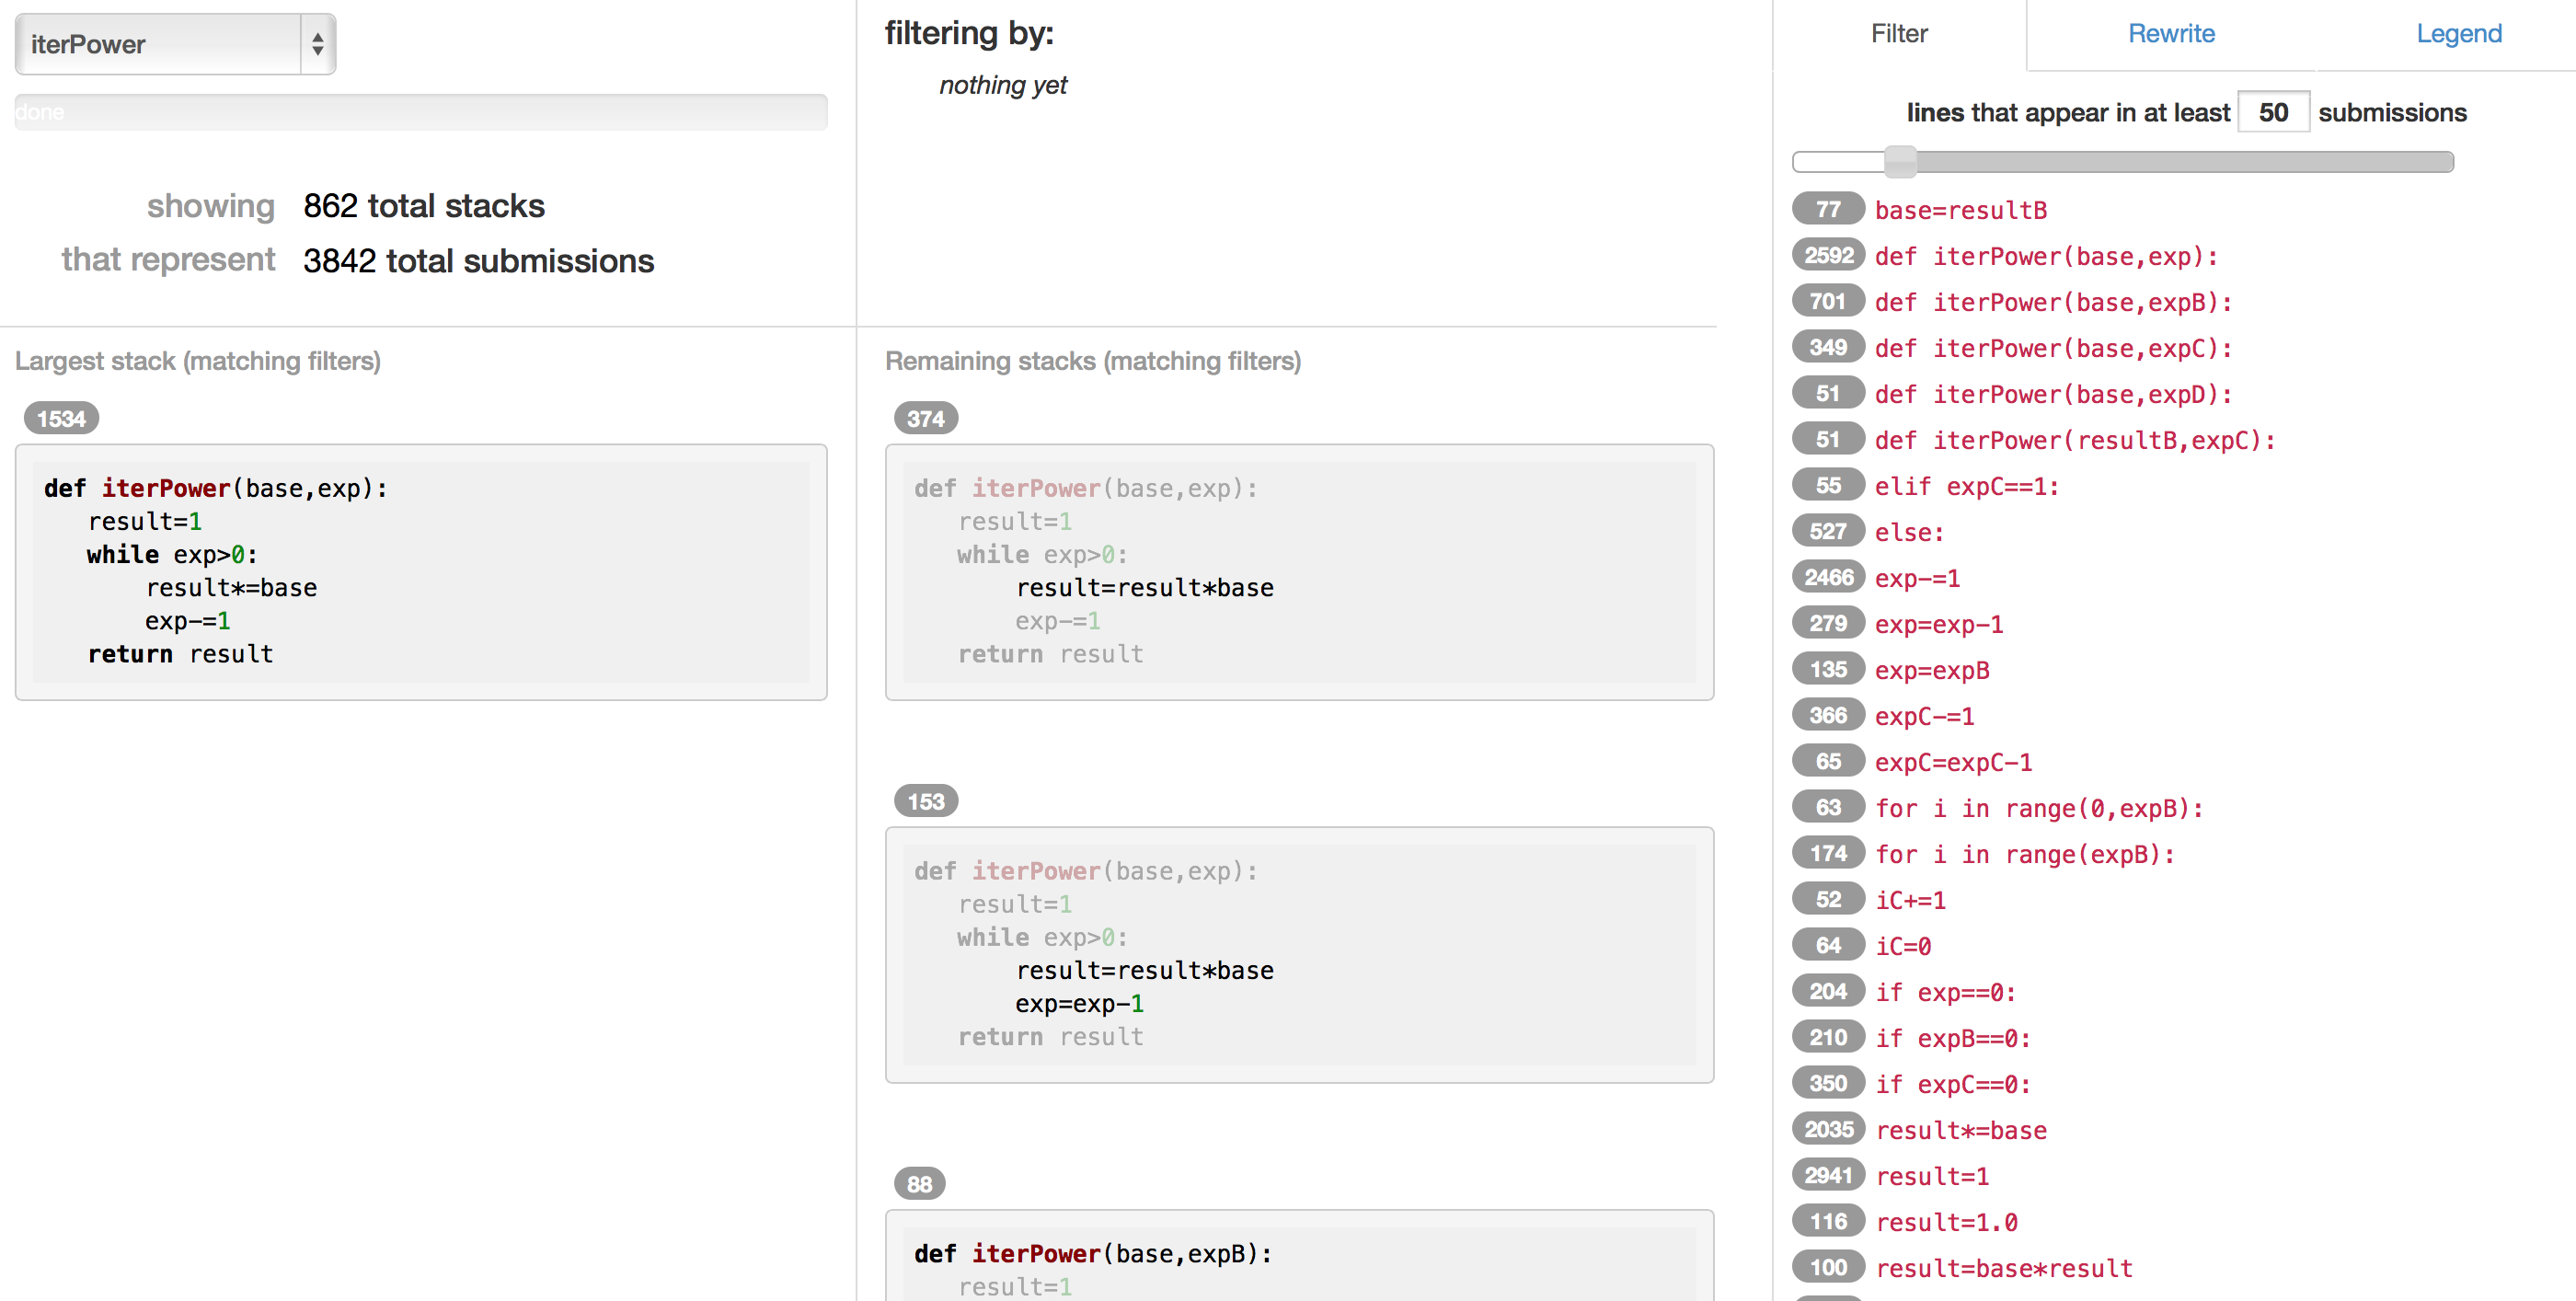
\includegraphics[width=1.0\linewidth]{Body/figures/overcode/interfaceScreenShot.png}
\caption{The OverCode user interface. The top left panel shows the number of clusters, called {\it stacks}, and the total number of solutions visualized. The next panel down in the first column shows the largest stack, while the second column shows the remaining stacks. The third column shows the lines of code in the platonic solutions and their frequencies.}
\label{overcode_fullinterface}
\end{figure*}

Sifting through thousands of solutions to understand their variation and find pedagogically valuable examples is a daunting task, even if the programming problems are simple and the solutions are only tens of lines of code long. Without tool support, a teacher may not read more than 50-100 of them before growing frustrated with the tedium of the task. Given this small sample size, teachers cannot be expected to develop a thorough understanding of the variety of strategies used to solve the problem, produce instructive feedback that is relevant to a large proportion of learners, or find unexpected interesting solutions.

An information visualization approach would enable teachers to explore the variation in solutions at scale. Existing techniques~\cite{gradingsigcse14,MOOCshop,codewebs} use a combination of clustering to group solutions that are semantically similar, and graph visualization to show the variation between these clusters. These clustering algorithms perform pairwise comparisons that are quadratic in both the number of solutions and in the size of each solution, which scales poorly to thousands of solutions. Graph visualization also struggles with how to label the graph node for a cluster, because it has been formed by a complex combination of code features. Without meaningful labels for clusters in the graph, the rich information in student solutions is lost and the ability of the teacher to understand variation is weakened.

This chapter presents OverCode, a system for visualizing and exploring the variation in thousands of programming solutions. OverCode is designed to visualize correct solutions, in the sense that they already passed the automatic grading tests typically used in a programming class at scale. The autograder cannot offer any further feedback on these correct solutions, and yet there may still be good and bad variations on correct solutions that are pedagogically valuable to highlight and discuss. OverCode aims to help teachers understand solution variation so that they can provide appropriate feedback to students at scale.

OverCode uses a novel human-interpretable solution clustering technique. The clustering process is linear in time with respect to both the number of solutions and the size of each solution. The platonic solution that represents each cluster is readable, executable, and describes every solution in that cluster in a deterministic way that accounts for both syntax and behavior on test cases. The platonic solutions are shown in a visualization that puts code front-and-center (Figure~\ref{overcode_fullinterface}). In the OverCode interface, teachers read through platonic solutions that each represent an entire cluster of solutions. The differences between clusters are highlighted to help teachers discover and understand the variations among solutions. Clusters can be filtered by the lines of code within them.  Clusters can also be merged together with {\em rewrite rules} that collapse variations that the teacher decides are unimportant. 

A cluster in OverCode is a set of solutions that perform the same computations, but may use different variable names or statement order.  OverCode uses a lightweight dynamic analysis to generate clusters, which scales linearly with the number of solutions. It clusters solutions whose variables take the same sequence of values when executed on test inputs and whose set of constituent lines of code are syntactically the same. 

An important component of this analysis is to rename variables that behave the same across different solutions. The renaming of variables serves three main purposes. First, it lets teachers create a mental mapping between variable names and their behavior which is consistent across the entire set of solutions. This may reduce the cognitive load for a teacher to understand different solutions. Second, it helps clustering by reducing variation between similar solutions. Finally, it also helps make the remaining differences between different solutions more salient. 

This chapter concludes by presenting two user studies with a total of 24 participants who each looked at thousands of solutions from an introductory programming MOOC, the OverCode interface is compared with a baseline interface that showed original unclustered solutions. When using OverCode, participants felt that they developed a better high-level view of the students' understandings and misconceptions. While participants did not necessarily read more lines of code in the OverCode interface than in the baseline, the code they did read came from clusters containing a greater percentage of all the submitted solutions. Participants also drafted mock class forum posts about common good and bad solutions. These forum posts were relevant to more student solutions when using OverCode as compared to the baseline. 

\section{OverCode} \label{overcode}
OverCode is an information visualization application for teachers to explore student solutions. OverCode uses the metaphor of solutions stacked on top of each other to denote a cluster of similar solutions. The top solution in the stack is the platonic solution that represents all the other solutions in the stack. The OverCode interface allows the teacher to scroll through, filter, and merge stacks of solutions. 

The platonic solutions that represent stacks are normalized in a novel way. Specifically, they have standardized formatting, no comments, and variable names that reflect the most popular naming choices across all solutions. They can be filtered by the normalized lines of code they contain and, through rewrite rules, modified and merged. They are the result of the normalization process applied to all student solutions in the OverCode analysis pipeline. %They can also be rewritten when teachers compose and apply \emph{rewrite rules}, which can eliminate differences between platonic solutions and therefore merge stacks that have become identical after the rewrite. 

%The OverCode interface was iteratively designed and developed based on continuous evaluation by the authors, feedback from teachers and peers, and by consulting principles from the information visualization literature. 
A screenshot of OverCode visualizing \codevar{iterPower}, one of the problems from our dataset, is shown in Figure~\ref{overcode_fullinterface}. In this section, the intended use cases and the user interface are described. In Section \ref{pipeline}, the backend program analysis pipeline is described in detail. 
\subsection{Target Users and Tasks}
The target users of OverCode are teaching staff of introductory programming courses. Teaching staff may be undergraduate lab assistants who help students debug their code; graduate students who grade assignments, help students debug, and manage recitations and course forums; and instructors who compose major course assessments. Teachers using OverCode may be looking for common misconceptions, creating a grading rubric, or choosing pedagogically valuable examples to review with students in a future lesson.

\subsubsection{Misconceptions and Holes in Student Knowledge}
Students just starting to learn programming can have a difficult time understanding the language constructs and different API methods. They may use them suboptimally, or in non-standard ways. OverCode may help instructors identify these common misconceptions and holes in knowledge, by highlighting the differences between stacks of solutions. Since the visualized solutions have already been tested and found correct by an autograder, these highlighted differences between platonic solutions may be convoluted variations in construct usage and API method choices that have not been flagged by the Python interpreter or caused the failure of a unit test. Convoluted code may suggest a misconception.

%\todo{DNHT: Rob: it would be great to show example code for these tasks, ideally showing them in OverCode -- can you mine any examples from your thesis defense talk?}

\subsubsection{Grading Rubrics}
It is a difficult task to create grading rubrics for checking properties such as design and style of solutions. Therefore most autograders resort to checking only functional correctness of solutions by testing them against a test suite of input-output pairs. OverCode enables teachers to identify the style, structure, and relative frequency of the variation within correct solutions. Unlike traditional ways of creating a grading rubric, where an instructor may go through a set of solutions, revising the rubric along the way, instructors can use OverCode to first get a high-level overview of the variations before designing a corresponding rubric. Teachers may also see incorrect solutions not caught by the autograder.

\subsubsection{Pedagogically Valuable Examples} 
There can be a variety of ways to solve a given problem and express it in code. If an assignment allows students to generate different solutions, e.g., recursive or iterative, to fulfill the same input-output behavior, OverCode will show separate stacks for each of these different solutions, as well as stacks for every variant of those solutions. OverCode helps teachers filter through solutions to find different examples of solutions to the same problem, which may be pedagogically valuable. According to variation theory ~\cite{marton13}, students can learn through concrete examples of these multiple solutions, which vary along different conceptual dimensions.
\subsection{User Interface}

The OverCode user interface is the product of an iterative design process with multiple stages, including paper prototypes and low-fidelity prototypes rendered in a web browser. User interface design experts and programming teachers critiqued initial prototypes. While exploring the low-fidelity prototypes, the teachers talked aloud about their hopes for what the tool could do, frustrations with its current form, and their frustrations with existing solution-viewing tools and processes. This feedback was incorporated into the final design.

The OverCode user interface is divided into three columns. The top-left panel in the first column shows the problem name, the \emph{done} progress bar, the number of stacks, the number of visualized stacks given the current filters and rewrite rules, and the total number of solutions those visualized stacks contain. The panel below shows the largest stack of solutions. Side by side with the largest stack, the remaining stacks appear in the second panel. Through scrolling, any stack can be horizontally aligned with the largest stack for easier comparison. The third panel has three different tabs that provide static and dynamic information about the solutions, and the ability to filter and combine stacks. 

As shown in Figure~\ref{overcode_fullinterface}, the default tab shows a list of lines of code that occur in different platonic solutions together with their corresponding frequencies. The stacks can be filtered based on the occurrence of one or more lines (Filter tab). The column also has tabs for \emph{Rewrite} and \emph{Legend}. The Rewrite tab allows a teacher to provide rewrite rules to collapse different stacks with small differences into a larger single stack. The Legend tab shows the dynamic values that different program variables take during the execution of programs over a test case. %We now describe different features of OverCode in more detail.
%\todo{ROB:maybe the TOCHI paper didn't have space for screenshots of these, but your thesis needs them}

% \begin{figure}
% 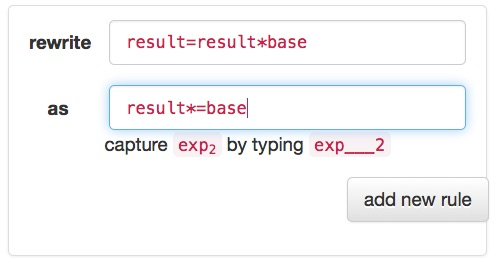
\includegraphics[width=0.5\paperwidth]{Body/figures/overcode/rewrite_rule.jpg}
% \caption{UI for adding rewrite rules.}
% \label{fig:rewriterule}
% \end{figure}

\subsubsection{Stacks} A stack in OverCode denotes a set of similar solutions that are grouped together based on a similarity criterion defined in Section \ref{pipeline}. For example, a stack for the \codevar{iterPower} problem is shown in Figure~\ref{stacks}(a). The size of each stack, i.e., the number of solutions in a stack, is shown in a pillbox at the top-left corner of the stack. Stacks are listed in the scrollable second panel from largest to smallest. The solution on the top of the stack is a platonic solution that describes all the solutions in the stack. See Section \ref{pipeline} for details on the normalizing process that produces platonic solutions.

Each stack can also be clicked. After clicking a stack, the border color of the stack changes and the \emph{done} progress bar is updated to reflect the percentage of total solutions clicked, as shown in Figure~\ref{stacks}(b). This feature is intended to help teachers remember which stacks they have already read or analyzed, and keep track of their progress. Clicking on a large stack, which represents a significant fraction of the total solutions, is reflected by a large change in the \emph{done} progress bar. Double clicking on any stack reveals the raw solutions that belong to that stack. This last feature was added after user testing.% \todo{add that now the raw solutions inside the stack are also displayed, but this was not included during user study tests}

\begin{figure*}[htpb]
\begin{tabular}{c | c}
\begin{minipage}{.5\linewidth}
\centering
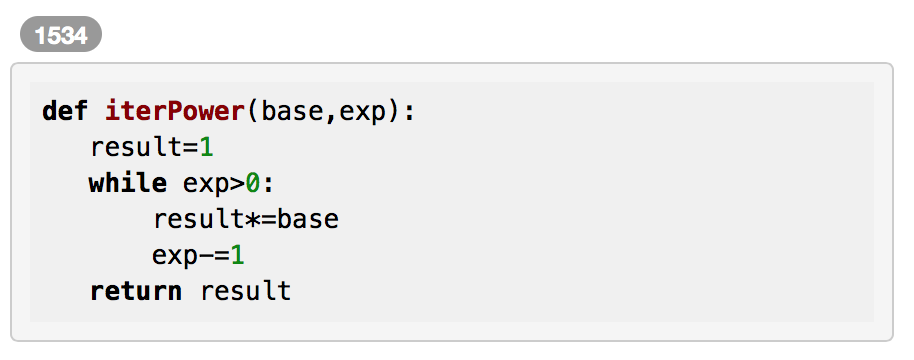
\includegraphics[width=0.95\linewidth]{Body/figures/overcode/stackScreenShot.png}
\end{minipage}
&
\begin{minipage}{.5\linewidth}
\centering
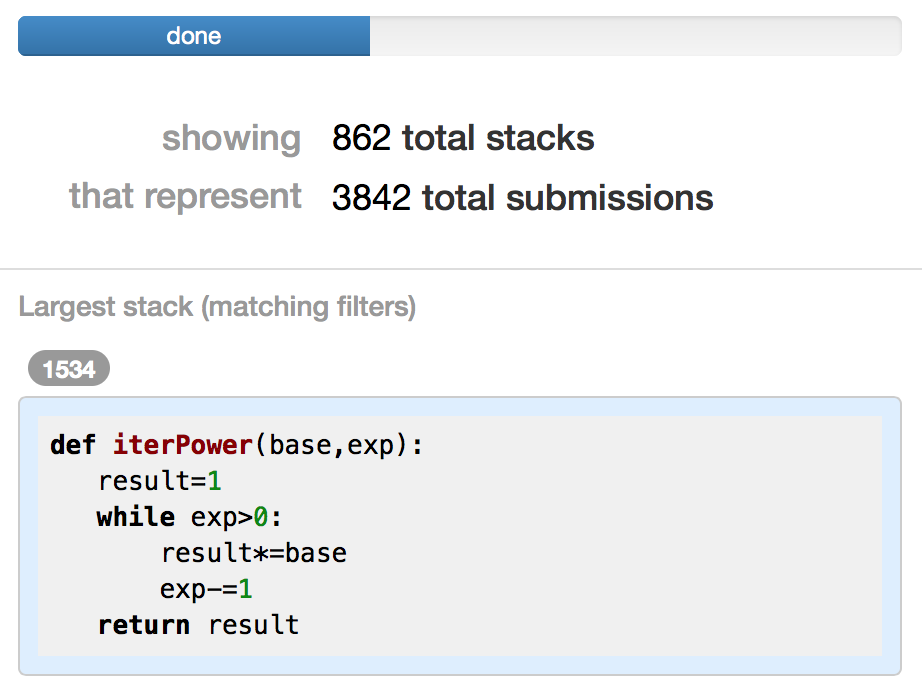
\includegraphics[width=0.95\linewidth]{Body/figures/overcode/checkDone.png}
\end{minipage}
\\
(a) & (b)
\end{tabular}
\caption{(a) A stack of 1534 similar \codevar{iterPower} solutions. (b) After clicking a stack, the border color of the stack changes and the done progress bar denotes the corresponding fraction of solutions that have been checked.}
\label{stacks}
\end{figure*}

\subsubsection{Showing Differences between Stacks} OverCode allows teachers to compare smaller stacks, shown in the second column, with the largest stack, shown in the first column. The lines of code in the second column that also appear in the set of lines in the largest stack are dimmed so that only the differences between the smaller stacks and the largest stack are apparent. For example, Figure~\ref{stackdifferences} shows the differences between the platonic solutions of the two largest stacks. In earlier iterations of the user interface, lines in stacks not shared with the largest stack were highlighted in yellow, but this produced a lot of visual noise. By dimming the lines in stacks that \textit{are} shared with the largest stack, the visible noise is reduced, while still keeping differences between stacks salient.

\begin{figure*}
\centering
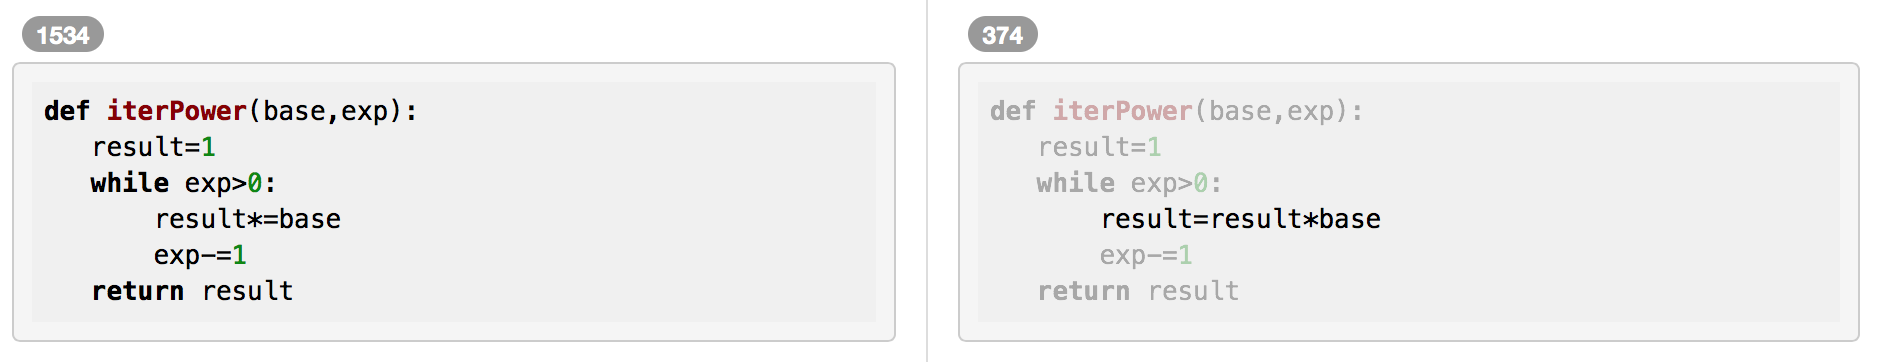
\includegraphics[scale=0.42]{Body/figures/overcode/lineFadingScreenshot}
\caption{Similar lines of code between two stacks are dimmed out such that only differences between the two stacks are apparent.}
\label{stackdifferences}
\end{figure*}



\subsubsection{Filtering Stacks by Lines of Code} The third column of OverCode shows the list of lines of code occurring in the solutions together with their frequencies (numbered pillboxes). The interface has a slider that can be used to change the threshold value, which denotes the number of solutions in which a line should appear for it to be included in the list. For example, by dragging the slider to $200$ in Figure~\ref{linefilter}(a), OverCode only shows lines of code that are present in at least $200$ solutions. This feature was added as a response to the length of the unfiltered list of code lines, which was long enough to make skimming for common code lines difficult.

Users can filter the stacks by selecting one or more lines of code from the list. After each selection, only stacks whose platonic solutions have those selected lines of code are shown. Figure~\ref{linefilter}(b) shows a filtering of stacks that have a \codevar{for} loop, specifically the line of code \codevar{for i in range(expB)}, and that assign $1$ to the variable \codevar{result}.

\begin{figure*}[htpb]
\begin{tabular}{c | c}
\begin{minipage}{.48\linewidth}
\centering
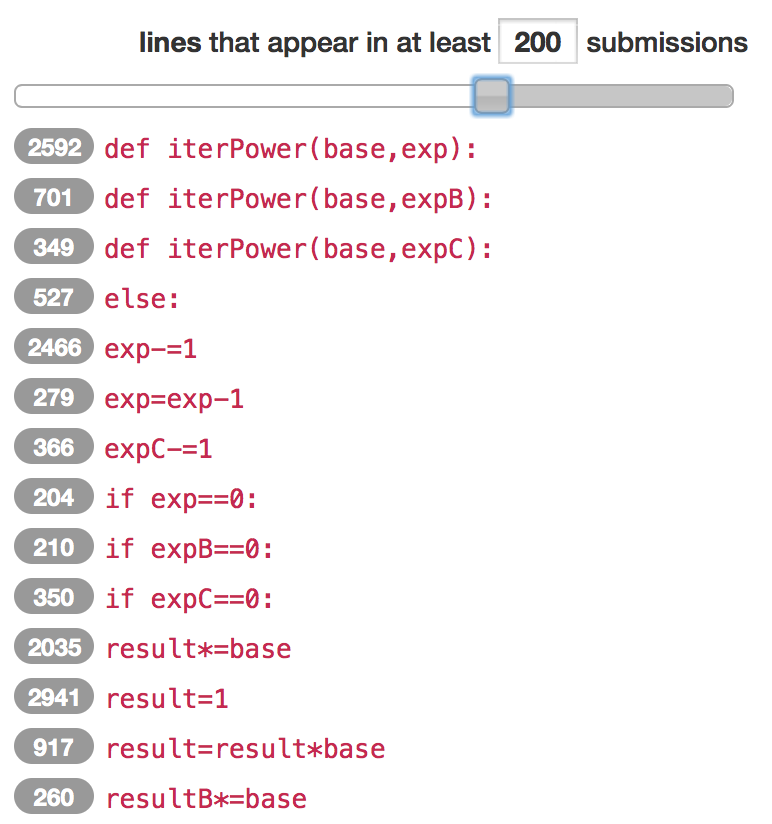
\includegraphics[scale=0.5]{Body/figures/overcode/lineSlider.png}
\end{minipage}
&
\begin{minipage}{.52\linewidth}
\centering
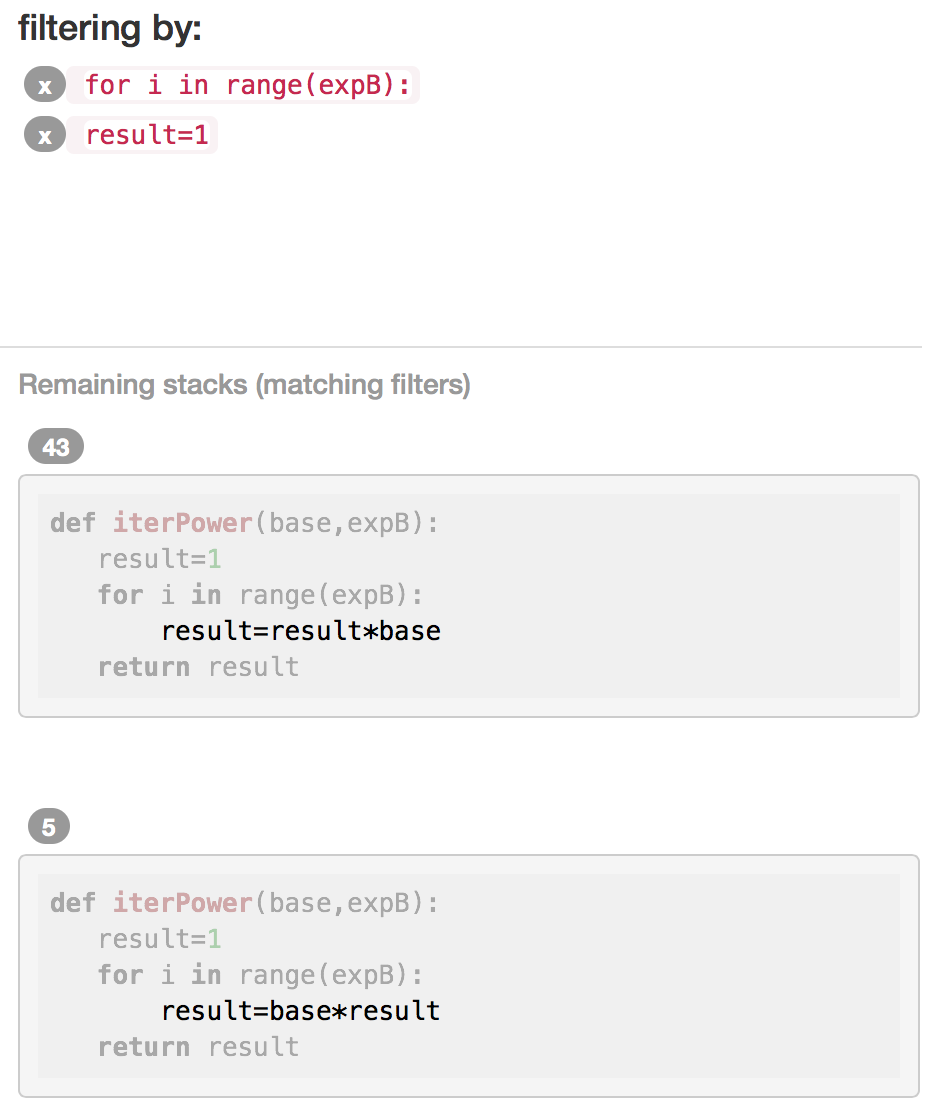
\includegraphics[scale=0.40]{Body/figures/overcode/lineFilter.png}
\end{minipage}
\\
(a) & (b)
\end{tabular}
\caption{(a) The slider allows filtering of the list of lines of code by the number of solutions in which they appear. (b) Clicking on a line of code adds it to the list of lines by which the stacks are filtered.}
\label{linefilter}
\end{figure*}

\subsubsection{Rewrite Rules} There are often small differences between the platonic solutions that can lead to a large number of stacks for a teacher to review. OverCode provides \emph{rewrite rules} by which teachers can collapse these differences and ignore variation they do not need to see. This feature comes from experience with early prototypes. After observing a difference between stacks, like the use of \codevar{xrange} instead of \codevar{range}, teachers wanted to ignore that difference in order to more easily find other differences.

A rewrite rule is described with a left hand side and a right hand side as shown in Figure~\ref{rewriterule}(a). The semantics of a rewrite rule is to replace all occurrences of the left-hand side expression in the platonic solutions with the corresponding right-hand side. As the rewrite rules are entered, OverCode presents a preview of the changes in the platonic solutions as shown in Figure~\ref{rewriterule}(b). After the application of the rewrite rules, OverCode collapses stacks that now have the same platonic solutions because of the rewrites. For example, after the application of the rewrite rule in Figure~\ref{rewriterule}(a), OverCode collapses the two biggest iterPower stacks from Figure~\ref{overcode_fullinterface} of sizes $1534$ and $374$, respectively, into a single stack of size $1908$. Other pairs of stacks whose differences have now been removed by the rewrite rule are also collapsed into single stacks. As shown in Figure~\ref{afterrewrite}(a), the number of stacks now drop from $862$ to $814$.

\begin{figure*}[htpb]
\begin{tabular}{c | c}
\begin{minipage}{.5\linewidth}
\centering
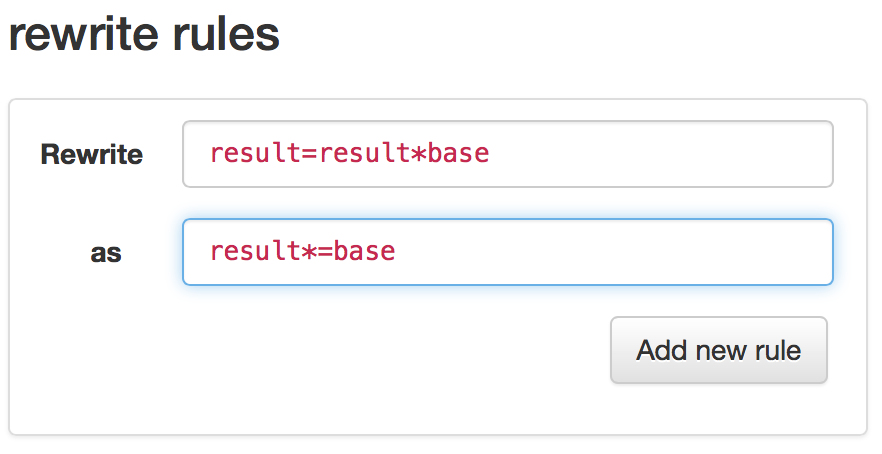
\includegraphics[scale=0.45]{Body/figures/overcode/rewriteRuleScreenshot.png}
\end{minipage}
&
\begin{minipage}{.5\linewidth}
\centering
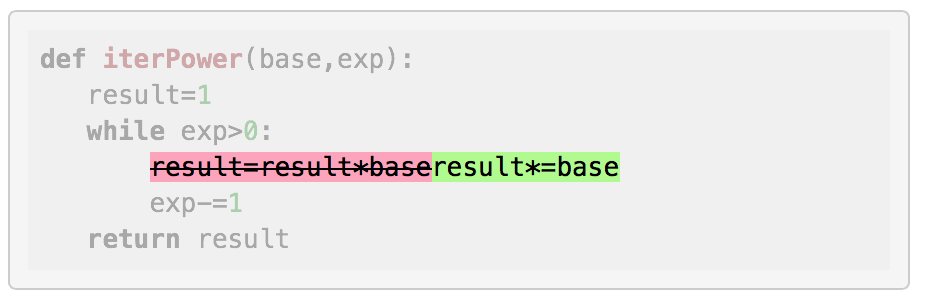
\includegraphics[scale=0.40]{Body/figures/overcode/rewritePreviewScreenShot.png}
\end{minipage}
\\
(a) & (b)
\end{tabular}
\caption{(a) An example rewrite rule to replace all occurrences of statement \codevar{result = base * result} with \codevar{result *= base}. (b) The preview of the changes in the platonic solutions because of the application of the rewrite rule.}
\label{rewriterule}
\end{figure*}

\begin{figure*}[htpb]
\begin{tabular}{c | c}
\begin{minipage}{.5\linewidth}
\centering
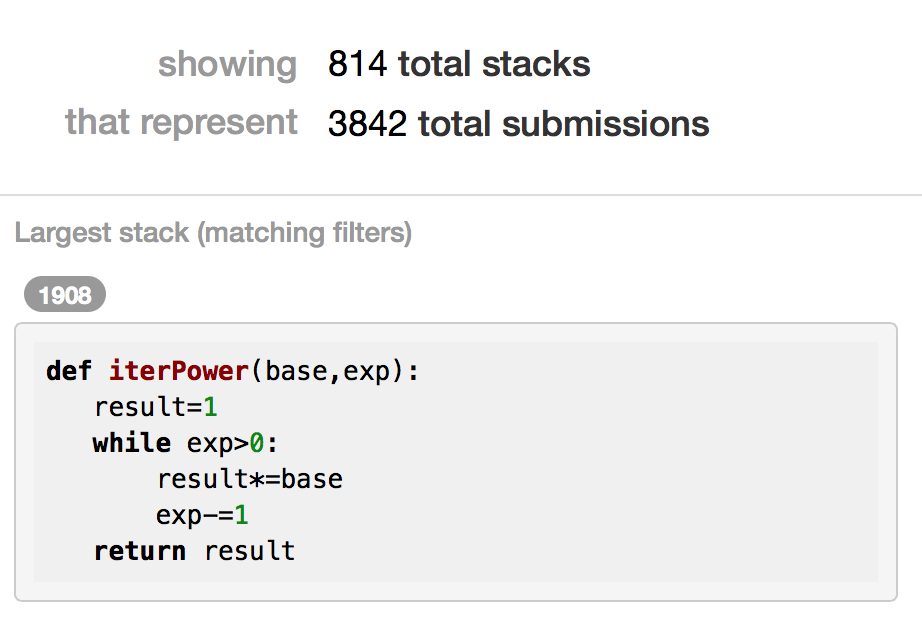
\includegraphics[scale=0.4]{Body/figures/overcode/afterrewrite.png}
\end{minipage}
&
\begin{minipage}{.5\linewidth}
\centering
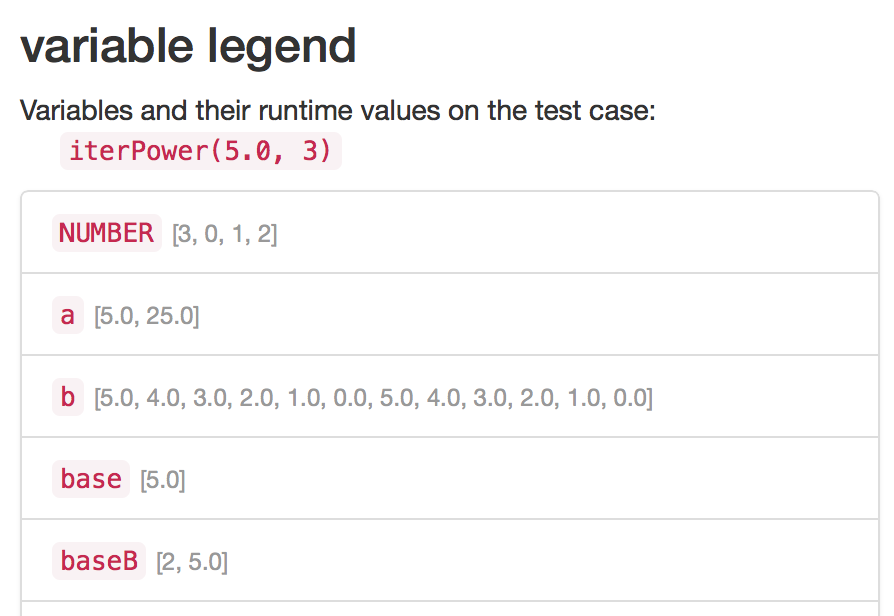
\includegraphics[scale=0.4]{Body/figures/overcode/variableLegend.png}
\end{minipage}
\\
(a) & (b)
\end{tabular}
\caption{(a) The merging of stacks after application of the rewrite rule shown in Figure~\ref{rewriterule}. (b) The variable legend shows the sequence of dynamic values that all program variables in normalized solutions take over the course of execution on a given test case.}
\label{afterrewrite}
\end{figure*}

\subsubsection{Variable Legends} OverCode also shows the sequence of values that variables in the platonic solutions take on, over the course of their execution on a test case. As described in Section~\ref{pipeline}, a variable is identified by the sequence of values it takes on during the execution of the test case. Figure~\ref{afterrewrite}(b) shows a snapshot of the variable values for the \codevar{iterPower} problem. The goal of presenting this dynamic information associated with common variable names is intended to help teachers (1) understand the behavior of each platonic solution without having to mentally execute it on a test case and (2) further explore the variations among solutions that do not have the same common variables. When this legend was originally added to the user interface, clicking on a common variable name would filter for all solutions that contained an instance of that variable. Some pilot users found this feature confusing, rather than empowering. As a result, it was removed from OverCode before running both user studies. At least one study participant, upon realizing the value of the legend, wished that the original click-to-filter-by-variable functionality existed; it may be reinstated in future versions.

\section{Implementation} \label{pipeline}
The OverCode user interface depends on an analysis pipeline that normalizes solutions in a manner designed for human readability. The pipeline then creates stacks of solutions that have become identical through the normalizing process. The pipeline accepts, as input, a set of solutions, expressed as function definitions for $f(a,...)$, and a set of test cases. Solutions that enter the pipeline are referred to as \emph{raw}, and the solutions that exit the pipeline as \emph{normal}. Examples, beginning with \codevar{iterPower}, are presented below to illustrate this pipeline.

\subsection{Analysis Pipeline}
OverCode is currently implemented for Python, but the pipeline steps described below could be readily generalized to other languages commonly used to teach programming.

{\bf 1. Reformat solutions.} For a consistent appearance, the solutions are reformatted with the PythonTidy package\footnote{Created by Charles Curtis Rhode. \url{https://pypi.python.org/pypi/PythonTidy/}} to have consistent line indentation and token spacing. Comments and empty lines are also removed. These steps not only make solutions more readable, but also allow exact string matches between solutions, after additional normalizing steps later in the pipeline. Although comments can contain valuable information, the variation in comments is so great that clustering and summarizing them will require significant additional design, which remains future work. Figure~\ref{fig:reformat} illustrates the effect of this reformatting.
\begin{figure}
\begin{tabular}{ll}
{\bf Raw Solution A} & {\bf Reformatted Solution A} \\
\begin{minipage}{0.5\linewidth}
\begin{lstlisting}[basicstyle=\linespread{1.0}\ttfamily\footnotesize,language=python]
def iterPower(base, exp):
    '''
    base: int or float.
    exp: int >= 0
    returns: int or float, base^exp
    '''
    result = 1
    for i in range(exp):
        result *= base
    return result
\end{lstlisting}
\end{minipage}
&
\begin{minipage}{0.5\linewidth}
\begin{lstlisting}[basicstyle=\linespread{1.0}\ttfamily\footnotesize,language=python]
def iterPower(base,exp):
    result=1
    for i in range(exp):
        result*=base
    return result
\end{lstlisting}
\end{minipage}
\end{tabular}
\caption{A student solution before and after reformatting.}
\label{fig:reformat}
\end{figure}

{\bf 2. Execute solutions.} Each solution is on the same test case(s). During each step of the execution for each test case, the names and values of local and global variables, and also return values from functions, are recorded as a program trace adapted from the execution logger written by Philip Guo~\cite{pgbovineOPT}. There is one program trace per solution per test case. Included for the purpose of illustrating this pipeline, the examples in the figures that follow are derived from executing definitions of \codevar{iterPower} on a \codevar{base} of $5.0$ and an \codevar{exp} of $3$, as illustrated in Figure~\ref{fig:testcase}.
\begin{figure}
\begin{tabular}{l}
{\bf Student Solution with Test Case} \\
\begin{minipage}{0.5\linewidth}
\begin{lstlisting}[basicstyle=\linespread{1.0}\ttfamily\footnotesize,language=python]
def iterPower(base,exp):
    #student solution here
iterPower(5.0, 3)
\end{lstlisting}
\end{minipage} 
\end{tabular}
\caption{Illustration of running a (dummy) \texttt{iterPower} solution on a test case.}
\label{fig:testcase}
\end{figure}

%This sequence of values excludes consecutive duplicates. 
{\bf 3. Extract variable sequences.} For each variable in a program trace, the pipeline extracts the sequence of distinct values it takes on. Figure~\ref{fig:extractsequence} shows the program trace for a solution run on a test case, as well as the extracted sequences of distinct values for each variable. Variable sequence extraction also works for purely functional programs, in which variables are never reassigned, because each recursive invocation is treated as if new values are given to its parameter variables. For example, in spite of the fact that the \codevar{iterPower} problem asked students to compute the exponential $\codevar{base}^\codevar{exp}$ iteratively, $60$ of the $3842$ \codevar{iterPower} solutions in the dataset were in fact recursive. One of these recursive examples is shown in Figure~\ref{fig:recursiveTrace}, along with the variable sequences extracted.
\begin{figure}
\begin{tabular}{ll}
{\bf Solution A with Test Case} & {\bf Program Trace for Solution A} \\
\begin{minipage}{0.35\linewidth}
\begin{lstlisting}[basicstyle=\linespread{1.0}\ttfamily\footnotesize,language=python]
def iterPower(base,exp):
    result=1
    for i in range(exp):
        result*=base
    return result
iterPower(5.0, 3)
\end{lstlisting}
\end{minipage} &
\begin{minipage}{0.6\linewidth}
\begin{lstlisting}[basicstyle=\linespread{1.0}\ttfamily\footnotesize,language=python,linebackgroundcolor={\lstcolorlines[gray!20]{2,4,6,8,10,12,14,16,18}}]
iterPower(5.0, 3)
 base : 5.0, exp : 3
result=1
 base : 5.0, exp : 3, result : 1 
for i in range(exp):
 base : 5.0, exp : 3, result : 1, i : 0
result*=base
 base : 5.0, exp : 3, result : 5.0, i : 0 
for i in range(exp):
 base : 5.0, exp : 3, result : 5.0, i : 1
result*=base 
 base : 5.0, exp : 3, result : 25.0, i : 1 
for i in range(exp):
 base : 5.0, exp : 3, result : 25.0, i : 2 
result*=base
 base : 5.0, exp : 3, result : 125.0, i : 2
return result
 value returned: 125.0
\end{lstlisting}
\end{minipage} 
\\
& {\bf Variable Sequences for Solution A} \\
&
\begin{minipage}{0.6\linewidth}
\begin{lstlisting}[language=python]
base: 5.0
exp: 3
result: 1, 5.0, 25.0, 125.0
i: 0, 1, 2
\end{lstlisting}
\end{minipage}
\end{tabular}
\caption{A student solution, its program trace when running on the test case \texttt{iterPower(5.0,3)}, and the sequence of values extracted from the trace for each variable.}
\label{fig:extractsequence}
\end{figure}

\begin{figure}
\begin{tabular}{ll}
{\bf Recursive Example} & {\bf Program Trace} \\
 % & {\bf for Recursive Example} \\
\begin{minipage}{0.5\linewidth}
\begin{lstlisting}[basicstyle=\linespread{1.0}\ttfamily\footnotesize,language=python]
def iterPower(base,exp):
   if exp==0:
       return 1
   else:
       return base*iterPower(base,exp-1)
iterPower(5.0, 3)
\end{lstlisting}
\end{minipage} &
\begin{minipage}{0.4\linewidth}
\begin{lstlisting}[basicstyle=\linespread{1.0}\ttfamily\footnotesize,language=python,linebackgroundcolor={\lstcolorlines[gray!20]{2,4,6,8,10,12,14,16,18,20,22,24,26,28,30}}]
iterPower(5.0, 3)
 base : 5.0, exp : 3
if exp==0:
 base : 5.0, exp : 3 
return base*iterPower(base,exp-1)
 base : 5.0, exp : 3 
iterPower(5.0, 2)
 base : 5.0, exp : 2
if exp==0: 
 base : 5.0, exp : 2 
return base*iterPower(base,exp-1)
 base : 5.0, exp : 2
iterPower(5.0, 1)
 base : 5.0, exp : 1
if exp==0:
 base : 5.0, exp : 1
return base*iterPower(base,exp-1)
 base : 5.0, exp : 1
iterPower(5.0, 0)
 base : 5.0, exp : 0
if exp==0:
 base : 5.0, exp : 0
return 1
 base : 5.0, exp : 0
return base*1
 base : 5.0, exp : 1
return base*5
 base : 5.0, exp : 2
return base*25
 base : 5.0, exp : 3
value returned: 125.0
\end{lstlisting}
\end{minipage} 
\\
& {\bf Variable Sequences} \\
% & {\bf for Recursive Example} \\
&
\begin{minipage}{0.5\linewidth}
\begin{lstlisting}[language=python]
base: 5.0
exp: 3, 2, 1, 0, 1, 2, 3
\end{lstlisting}
\end{minipage}
\end{tabular}
\caption{A recursive solution to the same programming problem, its program trace when executing on \texttt{iterPower(5.0,3)}, and the extracted sequences of values for each variable.}
\label{fig:recursiveTrace}
\end{figure}


{\bf 4. Identify common variables.} The pipeline analyzes all program traces, identifying which variable value sequences are identical. Variables that have identical sequences of values across two or more program traces are referred to as {\it common variables}. Variables which occur in only one program trace are called {\it unique variables}. This is illustrated in Figures~\ref{fig:commik} and~\ref{fig:allvars}.
\begin{figure}
\begin{tabular}{ll}
{\bf Solution B with Test Case} & {\bf Variable Sequences for Solution B} \\
\begin{minipage}{0.5\linewidth}
\begin{lstlisting}[basicstyle=\linespread{1.0}\ttfamily\footnotesize,language=python]
def iterPower(base,exp):
    r=1
    for k in xrange(exp):
        r=r*base
    return r
iterPower(5.0, 3)
\end{lstlisting}
\end{minipage}
&
\begin{minipage}{0.5\linewidth}
\begin{lstlisting}[language=python]
base: 5.0
exp: 3
r: 1, 5.0, 25.0, 125.0
k: 0, 1, 2
\end{lstlisting}
\end{minipage} \\
{\bf Solution C with Test Case} & {\bf Variable Sequences for Solution C} \\
\begin{minipage}{0.5\linewidth}
\begin{lstlisting}[basicstyle=\linespread{1.0}\ttfamily\footnotesize,language=python]
def iterPower(base,exp):
   result=1
   while exp>0:
       result*=base
       exp-=1
   return result
iterPower(5.0, 3)
\end{lstlisting}
\end{minipage}
&
\begin{minipage}{0.5\linewidth}
\begin{lstlisting}[language=python]
base : 5.0
exp: 3
result : 1, 5.0, 25.0, 125.0
exp : 3, 2, 1, 0
\end{lstlisting}
\end{minipage}
\end{tabular}
\caption{\codevar{i} and \codevar{k} take on the same sequence of values, $0$ then $1$ then $2$, in Solution A and B. They are therefore considered the same {\it common variable}.}
\label{fig:commik}
\end{figure}
\begin{figure}
{\bf Common variables} in solutions A, B, and C:
\begin{itemize}
\item \texttt{5.0}:
\begin{itemize}
\item \texttt{base} (Solutions A, B, C)
\end{itemize}
\item \texttt{3}:
\begin{itemize}
\item \texttt{exp} (Solutions A, B) 
\end{itemize}
\item \texttt{1, 5.0, 25.0, 125.0}: 
\begin{itemize}
\item \texttt{result} (Solutions A, C)
\item \texttt{r} (Student B)
\end{itemize}
\item \texttt{0,1,2}:
\begin{itemize}
\item \texttt{i} (Solution A) 
\item \texttt{k} (Student B)
\end{itemize}
\end{itemize}
{\bf Unique variables} in solutions A, B, and C:
\begin{itemize}
\item \texttt{3,2,1,0}:
\begin{itemize}
\item \texttt{exp} (Student C)
\end{itemize}
\end{itemize}
\caption{Common and uncommon variables found across the solutions in the previous figure.}
\label{fig:allvars}
\end{figure}

{\bf 5. Rename common and unique variables.} A common variable may have a different name in each program trace. In this step, the common variable is renamed to the name that is given most often to that common variable across all program traces. 

There are exceptions made to avoid name collisions. For example, the unique variable in the previous pipeline step was originally named \codevar{exp}. As shown in Figure~\ref{fig:uniqcomm}, OverCode appends a double underscore as a modifier to resolve a name collision with the common variable of the same name. This is referred to as a unique/common collision.
\begin{figure}
\begin{tabular}{ll}
{\bf Common Variables, Named} & {\bf Unique Variables, Named} \\
\begin{minipage}{0.5\linewidth}
\begin{itemize}
\item \texttt{base: 5.0} 
\item \texttt{exp: 3} 
\item \texttt{result: 1, 5.0, 25.0, 125.0}
\item \texttt{i: 0,1,2} (common name tie broken by random choice)
\end{itemize}
\end{minipage}
&
\begin{minipage}{0.5\linewidth}
\begin{itemize}
\item \begin{verbatim} exp__: 3,2,1,0 \end{verbatim}
\end{itemize}
\end{minipage}

\end{tabular}
\caption{The unique variable in the previous pipeline step was originally named \codevar{exp}. OverCode appends a double underscore as a modifier to resolve a name collision with the common variable of the same name. This is referred to as a unique/common collision.}
\label{fig:uniqcomm}
\end{figure}

After common and unique variables in the solutions are renamed, the solutions are now called {\it normal}, as shown in Figure~\ref{fig:normalcode}.
\begin{figure}
\begin{tabular}{ll}

{\bf Normal Solution A} & {\bf Normal Solution B} \\ 

\begin{minipage}{0.5\linewidth}
\begin{lstlisting}[basicstyle=\linespread{1.0}\ttfamily\footnotesize,language=python]
def iterPower(base,exp):
    result=1
    for i in range(exp):
        result*=base
    return result
\end{lstlisting}
\end{minipage} &
\begin{minipage}{0.5\linewidth}
\begin{lstlisting}[basicstyle=\linespread{1.0}\ttfamily\footnotesize,language=python]
def iterPower(base,exp):
    result=1
    for i in xrange(exp):
        result=result*base
    return result
\end{lstlisting}
\end{minipage}
\\
{\bf Normal Solution C} &  \\
\begin{minipage}{0.5\linewidth}
\begin{lstlisting}[basicstyle=\linespread{1.0}\ttfamily\footnotesize,language=python]
def iterPower(base,exp__):
   result=1
   while exp__>0:
       result*=base
       exp__-=1
   return result
\end{lstlisting}
\end{minipage}
& \\
\end{tabular}
\caption{Normalized solutions after variable renaming.}
\label{fig:normalcode}
\end{figure}

{\bf 6. Make stacks.} The pipeline iterates through the normal solutions, making stacks of solutions that share an identical {\it set} of lines of code. The pipeline compares sets of lines of code because then solutions with arbitrarily ordered lines that do not depend on each other can still fall into the same stack. (Recall that the variables in these lines of code have already been renamed based on their dynamic behavior, and all the solutions have already been marked input-output correct by an autograder, prior to this pipeline.) The platonic solution that represents the stack is randomly chosen from within the stack, because all the normal solutions within the stack are identical, with the possible exception of the order of their statements. 

In the examples in Figure~\ref{fig:makingstacks}, the normal C and D solutions have the same set of lines, and both provide correct output, with respect to the autograder. Therefore, the difference in order of the statements between the two solutions is not communicated to the teacher. The two solutions are put in the same stack, with one solution arbitrarily chosen as the visible normalized code. However, since Solution A and B use different functions, i.e., \codevar{xrange} vs. \codevar{range}, and different operators, i.e., \codevar{*=} vs. \codevar{=,*}, the pipeline puts them in separate stacks.
%\vspace{10mm}
\begin{figure}
\begin{tabular}{l|l}
{\bf Stack 1} Normal Solution A & {\bf Stack 2} Normal Solution B \\
\begin{minipage}{0.5\linewidth}
\begin{lstlisting}[basicstyle=\linespread{1.0}\ttfamily\footnotesize,language=python,linebackgroundcolor={\lstcolorlines[gray!20]{3,4}}]
def iterPower(base,exp):
    result=1
    for i in range(exp):
        result*=base
    return result
\end{lstlisting}
\end{minipage}
&
\begin{minipage}{0.5\linewidth}
\begin{lstlisting}[basicstyle=\linespread{1.0}\ttfamily\footnotesize,language=python,linebackgroundcolor={\lstcolorlines[gray!20]{3,4}}]
def iterPower(base,exp):
    result=1
    for i in xrange(exp):
        result=result*base
    return result
\end{lstlisting}
\end{minipage}
\end{tabular}
\begin{tabular}{ll}
\hline
\\
{\bf Stack 3} Normal Solution C & {\bf Stack 3} Normal Solution D  \\
\begin{minipage}{0.5\linewidth}
\begin{lstlisting}[basicstyle=\linespread{1.0}\ttfamily\footnotesize,language=python,linebackgroundcolor={\lstcolorlines[mygray]{4,5}}]
def iterPower(base,exp__):
    result=1
    while exp__>0:
        result=result*base
        exp__-=1
    return result
\end{lstlisting}
\end{minipage}
&
\begin{minipage}{0.5\linewidth}
\begin{lstlisting}[basicstyle=\linespread{1.0}\ttfamily\footnotesize,language=python,linebackgroundcolor={\lstcolorlines[mygray]{4,5}}]
def iterPower(base,exp__):
    result=1
    while exp__>0:
        exp__-=1
        result=result*base
    return result
\end{lstlisting}
\end{minipage}
\end{tabular}
\caption{Four solutions collapsed into three stacks.}
\label{fig:makingstacks}
\end{figure}
Some programming problems have no deadline, and new solutions are submitted intermittently. The entire pipeline does not need to be rerun to normalize a new solution and restack all the solutions in the dataset. The pipeline has been split into two phases: solution preprocessing and batch processing. During preprocessing, each solution formatting is standardized and all comments are removed. It is then executed on one or more test cases, which makes the resulting normalization more robust to any individual poorly chosen test case. The full program trace and output is recorded for every test case. 

This logging of solution execution can be one of the longer steps in the OverCode analysis pipeline, so preprocessing occurs once per solution and is saved in its own pickle file. New solutions can be preprocessed once, without affecting previously preprocessed solutions. Batch processing takes, as input, all the existing preprocessed results and normalizes variable names. This must occur as a batch operation because variable renaming depends on the behavior and name of every variable in every solution.

The program tracing \cite{pgbovineOPT} and renaming scripts occasionally generate errors while processing a solution. For example, the script may not have code to handle a particular but rare Python construct. Errors thrown by the scripts drive their development and are helpful for debugging. When errors occur while processing a particular solution, they are excluded from our analysis. Less than five percent of the solutions in each of the three problem datasets are excluded.

\subsection{Variable Renaming Details and Limitations} \label{repercussions}

There are three distinct types of name collisions possible when renaming variables to be consistent across multiple solutions. The first, referred to here as a {\it common/common} collision, occurs when two common variables (with different variable sequences) have the same common name. The second, referred to here as a {\it multiple instances} collision, occurs when there are multiple different instances of the same common variable in a solution. The third and final collision, referred to as a {\it unique/common} collision, occurs when the name of a unique variable collides with the name of a common variable.

{\bf Common/common collision.} If common variables $cv_{1}$ and $cv_{2}$ are both most frequently named $i$ across all program traces, the pipeline appends a modifier to the name of the less frequently used common variable. For example, if 500 program traces have an instance of $cv_{1}$ and only 250 program traces have an instance of $cv_{2}$, $cv_{1}$ will be named $i$ and $cv_{2}$ will be named $iB$.  

For example, a subset of \codevar{iterPower} solutions created a variable that iterated through the values generated by \codevar{range(exp)}. Solution A is an example. A smaller subset created a variable that iterated through the values generated by \codevar{range(1,exp+1)}, as seen in Solution E. These are two separate common variables in our pipeline, due to their differing value sequences. The {\it common/common} name collision arises because both common variables are most frequently named \codevar{i} across all solutions to \codevar{iterPower}. To preserve the one-to-one mapping of variable name to value sequence across the entire \codevar{iterPower} problem dataset, the pipeline appends a modifier, \codevar{B}, to the common variable \codevar{i} found in fewer \codevar{iterPower} solutions. A common variable, also most commonly named \codevar{i}, which is found in even fewer \codevar{iterPower} definitions, will have a \codevar{C} appended, etc. This is illustrated in Figure~\ref{fig:commcommcoll}.
\begin{figure}
\begin{tabular}{l|l}

{\bf Solution A (Represents 500 Solutions)} & {\bf Solution E (Represents 250 Solutions)} \\
\begin{minipage}{0.5\linewidth}
\begin{lstlisting}[basicstyle=\linespread{1.0}\ttfamily\footnotesize,language=python]
def iterPower(base,exp):
    result=1
    for i in range(exp):
        result*=base
    return result
\end{lstlisting}
\end{minipage}
&
\begin{minipage}{0.5\linewidth}
\begin{lstlisting}[basicstyle=\linespread{1.0}\ttfamily\footnotesize,language=python,linebackgroundcolor={\lstcolorlines[gray!20]{3}}]
def iterPower(base,exp):
   result=1
   for i in range(1,exp+1):
       result*=base
   return result
\end{lstlisting}
\end{minipage}
\\
{\bf Normal Solution A (After Renaming)} & {\bf Normal Solution E (After Renaming)} \\
\codevar{(unchanged)} 
&
\begin{minipage}{0.5\linewidth}
\begin{lstlisting}[basicstyle=\linespread{1.0}\ttfamily\footnotesize,language=python,linebackgroundcolor={\lstcolorlines[gray!20]{3}}]
def iterPower(base,exp):
   result=1
   for iB in range(1,exp+1):
       result*=base
   return result
\end{lstlisting}
\end{minipage}
\end{tabular}
\caption{The top row illustrates a name collision of two common variables, both most commonly named \texttt{i}, across two stacks. The second row illustrates how the colliding variable name in the smaller stack of solutions is modified with an appended character to resolve the collision.}
\label{fig:commcommcoll}
\end{figure}

{\bf Multiple-instances collision.} The pipeline identifies variables by their sequence of values. This representation does not preserve information about the timing of when one value transitions to the next, relative to the values of other variables. Without those relative transition times, it is not possible to differentiate between multiple instances of a common variable within a single solution or identically behaving, semantically distinct Boolean flags in different solutions. This is not a fundamental limitation of this method, because this information is in the program trace. Future versions of OverCode could extract it as well.

Rather than injecting a name collision into an otherwise correct solution, the pipeline preserves the variable name chosen by the student for all the instances of that common variable in that solution. If the student-chosen name collides with any common variable name in any program trace and does not share its sequence of values, the pipeline appends a double underscore to the student-chosen name, so that both the interface and the human reader do not conflate them.

In Figure~\ref{fig:multiinst}, the solution author made a copy of the \codevar{exp} variable, called it \codevar{exp1}, and modified neither. Both map to the same common variable, \codevar{expB}. Therefore, both have had their author-given names preserved, with an underscore appended to the local \codevar{exp} so it does not look like common variable \codevar{exp}. 
\begin{figure}
\begin{tabular}{ll}
{\bf Solution with Multiple Instances} & {\bf Common Variable Mappings} \\
{\bf of a Common Variable} & \\
\begin{minipage}{0.4\linewidth}
\begin{lstlisting}[basicstyle=\linespread{1.0}\ttfamily\footnotesize,language=python]
def iterPower(base,exp):
   result=1
   exp1=abs(exp)
   for i in xrange(exp1):
       result*=base
   if exp<0:
       return 1.0/float(result)
   return result
iterPower(5.0,3)
\end{lstlisting}
\end{minipage}
&
\begin{minipage}{0.6\linewidth}
\begin{lstlisting}[basicstyle=\linespread{1.0}\ttfamily\footnotesize]
Both exp and exp1 map to
common variable expB:
exp: 3 
exp1: 3 

All other variables map to
common variables of same name:
base: 5.0 
i: 0, 1, 2 
result: 1, 5.0, 25.0, 125.0 
\end{lstlisting}
\end{minipage} \\
{\bf Solution with Multiple Instances Collision Resolved} & \\
\begin{minipage}{0.4\linewidth}
\begin{lstlisting}[basicstyle=\linespread{1.0}\ttfamily\footnotesize,language=python,linebackgroundcolor={\lstcolorlines[gray!20]{1,3,6}}]
def iterPower(base,exp__):
   result=1
   exp1=abs(exp__)
   for i in xrange(exp1):
       result*=base
   if exp__<0:
       return 1.0/float(result)
   return result
iterPower(5.0,3)
\end{lstlisting}
\end{minipage}
& \\
\end{tabular}
\caption{A variable name in a solution with multiple instances of a common variable, i.e., a multiple-instances collision, is modified so that its behavior during execution is unchanged.}
\label{fig:multiinst}
\end{figure}

{\bf Unique/common collision.} Unique variables, as defined before, take on a sequence of values that is unique across all program traces. If the name of a unique variable collides with the name of any common variable in any program trace, the pipeline appends a double underscore to the name of the unique variable, so that the interface and the human reader do not conflate them. 

%In addition to the example of this collision in the description of common and variable naming in the previous section, we provide the example below. 
In Figure~\ref{fig:lastone}, the student added $1$ to the exponent variable before entering a \codevar{while} loop. No other students did this. To indicate that the \codevar{exp} variable is {\it unique} and does not share the same behavior as the common variable also named \codevar{exp}, our pipeline appends double underscores to \codevar{exp} in this one solution. 

%{\bf Student Code with Unique Variable}
\begin{figure}
\begin{minipage}{0.45\linewidth}
\begin{lstlisting}[basicstyle=\linespread{1.0}\ttfamily\footnotesize,language=python,linebackgroundcolor={\lstcolorlines[gray!20]{1,3,4,6}}]
def iterPower(base,exp__):
   result=1
   exp__+=1
   while exp__>1:
       result*=base
       exp__-=1
   return result
\end{lstlisting}
\end{minipage}
\caption{A student solution with a unique variable, originally named \texttt{exp} by the student. Since it does not share the same behavior with the common variable also named \texttt{exp}, OverCode appends two underscores to the name of the unique variable, \texttt{exp}, to distinguish it.}
\label{fig:lastone}
\end{figure}



\subsection{Complexity of the Analysis Pipeline}\label{complexity}
Clustering methods that use pairwise AST edit distance metrics have quadratic complexity both in the number of solutions and the size of the ASTs~\cite{MOOCshop}. The OverCode analysis pipeline has linear complexity in the number of solutions and in the size of the ASTs. The Reformat step performs a single pass over each solution for removing extra spaces, comments, and empty lines. Given the assumption that all solutions in the pipeline are correct, each solution can be executed within a constant time that is independent of the number of solutions. The executions performed by the autograder for checking correctness could also be instrumented to obtain the program traces, so code is not unnecessarily re-executed. The identification of all common variables and unique variables across the program traces takes linear time as the corresponding variable sequences can be hashed and then checked for occurrences of identical sequences. The Renaming step, which includes handling name collisions, also performs a single pass over each solution. Finally, the Stacking step creates stacks of similar solutions by testing set equality, which can be performed in linear time by hashing the sets.


\section{Dataset} \label{dataset}

For evaluating both the analysis pipeline and the user interface of OverCode, the dataset of solutions is collected from 6.00x, an introductory programming course in Python that was offered on edX in fall 2012. Three programming problems were chosen. This dataset consists of student solutions submitted within two weeks of the release date of each problem. There are thousands of solutions to these problems in the dataset. All solutions marked as correct by an autograder were passed on to OverCode for analysis. The number of solutions analyzed for each problem is shown in Figure~\ref{overcode_solutioncounttable}.



%\caption{Our dataset of problems from an introductory programming course in Python, from Fall 2012.}
%\label{table-edx-probs}

\begin{itemize}
\item {\bf \codevar{iterPower}} The \codevar{iterPower} problem asks students to write a function to compute the exponential $\codevar{base}^\codevar{exp}$ iteratively using successive multiplications. This was an in-lecture exercise for the lecture on teaching iteration. See Figure \ref{ipexamples} for examples.
\item {\bf \codevar{hangman}} The \codevar{hangman} problem takes a string \codevar{secretWord} and a list of characters \codevar{lettersGuessed} as input, and asks students to write a function that returns a string where all letters in \codevar{secretWord} that are not present in the list \codevar{lettersGuessed} are replaced with an underscore. This was a part of the third week of problem set problems. See Figure \ref{hmexamples} for examples.
\item {\bf \codevar{compDeriv}} The \codevar{compDeriv} problem requires students to write a Python function to compute the derivative of a polynomial, where the coefficients of the polynomial are represented as a Python list. This was also a part of the third week of problem set problems. See Figure \ref{cdexamples} for examples.
\end{itemize}

The three programming problems represent the typical problems students solve in the early weeks of an introductory programming course. The three problems have varying levels of complexity and ask students to perform loop computation over three fundamental Python data types, integers (\codevar{iterPower}), strings (\codevar{hangman}), and lists (\codevar{compDeriv}). The problems span the second and third weeks of the course in which they were assigned.

\begin{figure*}
{\begin{center}
\begin{tabular} {|l|r|r|}

\hline
\tabhead{Problem Description} & \tabhead{Total Submissions} & \tabhead {Correct Solutions} \\ \hline \hline
\codevar{iterPower} & 8940 & 3875 \\ \hline
\codevar{hangman} & 1746 & 1118 \\ \hline
\codevar{compDeriv} & 3013 & 1433 \\ \hline
\end{tabular}
\end{center}}
\caption{Number of solutions for the three problems in our 6.00x dataset.}
\label{overcode_solutioncounttable}
\end{figure*}

\begin{figure*}
{\bf IterPower Examples} \\
\begin{tabular}{cc} 
\begin{minipage}{0.4\linewidth}
\begin{lstlisting}[]
def iterPower(base, exp):
    result=1
    i=0
    while i < exp:
        result *= base
        i += 1
    return result
\end{lstlisting}
\end{minipage}
&
\begin{minipage}{0.4\linewidth}
\begin{lstlisting}[]
def iterPower(base, exp):
    t=1
    for i in range(exp):
        t=t*base
    return t
\end{lstlisting}
\end{minipage}
\\
\end{tabular}

\begin{tabular}{c c}
\begin{minipage}{0.4\linewidth}
\begin{lstlisting}]
def iterPower(base, exp):
    x = base
    if exp == 0:
        return 1
    else:
        while exp >1:
            x *= base
            exp -=1
        return x
\end{lstlisting}
\end{minipage}
&
\begin{minipage}{0.4\linewidth}
\begin{lstlisting}]
def iterPower(base, exp):
    x = 1
    for n in [base] * exp:
        x *= n
    return x
\end{lstlisting}
\end{minipage}

\end{tabular}
\caption{Example solutions for the \codevar{iterPower} problem in our 6.00x dataset.}
\label{ipexamples}
\end{figure*}


\begin{figure*}
{\bf Hangman Examples} \\
\begin{tabular}{c}
\begin{minipage}{1.0\linewidth}
\begin{lstlisting}[]

def getGuessedWord(secretWord, lettersGuessed):
    guessedWord = ''
    guessed = False
    for e in secretWord:
        for idx in range(0,len(lettersGuessed)):
            if (e == lettersGuessed[idx]):
                guessed = True
                break
        # guessed = isWordGuessed(e, lettersGuessed)
        if (guessed == True):
            guessedWord = guessedWord + e
        else:
            guessedWord = guessedWord + '_ '
        guessed = False
    return guessedWord
\end{lstlisting}
\end{minipage}
\\
\begin{minipage}{1.0\linewidth}
\begin{lstlisting}[]
def getGuessedWord(secretWord, lettersGuessed):
    if len(secretWord) == 0:
        return ''
    else:
        if lettersGuessed.count(secretWord[0]) > 0:
            return secretWord[0] + ' ' + getGuessedWord(secretWord[1:], lettersGuessed)
        else:
            return '_ ' + getGuessedWord(secretWord[1:], lettersGuessed)
\end{lstlisting}
\end{minipage}
\end{tabular}
\caption{Example solutions for the \codevar{hangman} problem in our 6.00x dataset.}
\label{hmexamples}
\end{figure*}
\begin{figure*}
{\bf CompDeriv Examples}\\
\begin{tabular}{cc} 
\begin{minipage}{0.5\linewidth}
\begin{lstlisting}[]
def computeDeriv(poly):
    der=[]
    for i in range(len(poly)):
        if i>0:
            der.append(float(poly[i]*i))
    if len(der)==0:
        der.append(0.0)
    return der

\end{lstlisting}
\end{minipage}
&
\begin{minipage}{0.5\linewidth}
\begin{lstlisting}[]
def computeDeriv(poly):
    if len(poly) == 1:
        return [0.0]
    fp = poly[1:]
    b = 1
    for a in poly[1:]:
        fp[b-1] = 1.0*a*b
        b += 1
    return fp
\end{lstlisting}
\end{minipage}
\\
\end{tabular}
\begin{tabular}{c c}
\begin{minipage}{0.4\linewidth}
\begin{lstlisting}[]
def computeDeriv(poly):
    if len(poly) < 2:
        return [0.0]
    poly.pop(0)
    for power, value in enumerate(poly):
        poly[power] = value * (power + 1)
    return poly
\end{lstlisting}
\end{minipage}
&
\begin{minipage}{0.4\linewidth}
\begin{lstlisting}[]
def computeDeriv(poly):
    index = 1
    polyLen = len(poly)
    result = []
    while (index < polyLen):
        result.append(float(poly[index]*index))
        index += 1
    if (len(result) == 0):
        result = [0.0]
    return result
\end{lstlisting}
\end{minipage}

\end{tabular}
\caption{Example solutions for the \codevar{compDeriv} problem in our 6.00x dataset.}
\label{cdexamples}
\end{figure*}


\section{OverCode Analysis Pipeline Evaluation}
We now present the evaluation of the OverCode analysis pipeline implementation on our Python dataset. We first present the running time of our algorithm and show that it can generate stacks within a few minutes for each problem on a laptop. We then present the distribution of initial stack sizes generated by the pipeline. Finally, we present some examples of the common variables identified by the pipeline and report on the number of cases where name collisions are handled during the normalizing process. The evaluation was performed on a Macbook Pro 2.6GHz Intel Core i7 with 16GB of RAM. %\todo{remove we's} 

{\bf Running Time} The complexity of the pipeline that generates stacks of solutions grows linearly in the number of solutions as described in Section~\ref{complexity}. Figure~\ref{backendevaluation} reports the running time of the pipeline on the problems in the dataset as well as the number of stacks and the number of common variables found across each of the problems. As can be seen from the Figure, the pipeline is able to normalize thousands of student solutions and generate stacks within a few minutes for each problem.

\begin{figure*}[htpb]
\centering
\begin{tabular}{|l|r|r|r|r|}
\hline
\multirow{2}{*}{\bf Problem} & {\bf Correct} & {\bf Running} & {\bf Initial} & {\bf Common }\\
& {\bf Solutions} & {\bf Time } & {\bf Stacks} & {\bf Variables}\\
\hline\hline
\codevar{iterPower} & 3875 & 15m 28s & 862 & 38\\ \hline
\codevar{hangman} & 1118 & 8m 6s & 552 & 106\\ \hline
\codevar{compDeriv} & 1433 & 10m 20s & 1109 & 50\\ \hline
\end{tabular}
\caption{Running time and the number of stacks and common variables generated by the OverCode backend implementation on our dataset problems.}
\label{backendevaluation}
\end{figure*}

{\bf Distribution of Stacks} The distribution of initial stack sizes generated by the analysis pipeline for different problems is shown in Figure~\ref{stackdistribution}. Note that the two axes of the graph corresponding to the size and the number of stacks are shown on a logarithmic scale. For each problem, we observe that there are a few large stacks and a lot of smaller stacks (particularly of size 1). The largest stack for \codevar{iterPower} problem consists of $1534$ solutions, while the largest stacks for \codevar{hangman} and \codevar{compDeriv} consist of $97$ and $22$ solutions, respectively. The two largest stacks for each problem are shown in Figure~\ref{toptwostacks}. 

The number of stacks consisting of a single solution for \codevar{iterPower}, \codevar{hangman}, and \codevar{compDeriv} are $684$, $452$, and $959$, respectively. Some singleton stacks are the same as one of the largest stacks, except for a unique choice, such as initializing a variable using several more significant digits than necessary: \codevar{result=1.000} instead of \codevar{result=1} or \codevar{result=1.0}. Other singleton stacks have convoluted control flow that no other student used. 

These variations are compounded by inclusion of unnecessary statements that do not affect input-output behavior. An existing stack may have all the same lines of code except for the unnecessary line(s), which cause the solution to instead be a singleton. These unnecessary lines may reveal misconceptions, and therefore are potentially interesting to teachers. In future versions, rewrite rules may be expanded to include line removal rules, so that teachers can remove inconsequential extra lines and cause singleton(s) to merge with other stacks. 

The tail of singleton solutions is long, and cannot be read in its entirety by teachers. Even so, the user studies indicate that teachers still extracted significant value from OverCode presentation of solutions. It may be that the largest stacks are the primary sources of information, and singletons can be ignored without a significant effect on the value teachers get from OverCode. Future work will explore ways to suggest rewrite and removal rules that maximally collapse stacks.

\begin{figure*}
\centering
\begin{tabular}{c c}
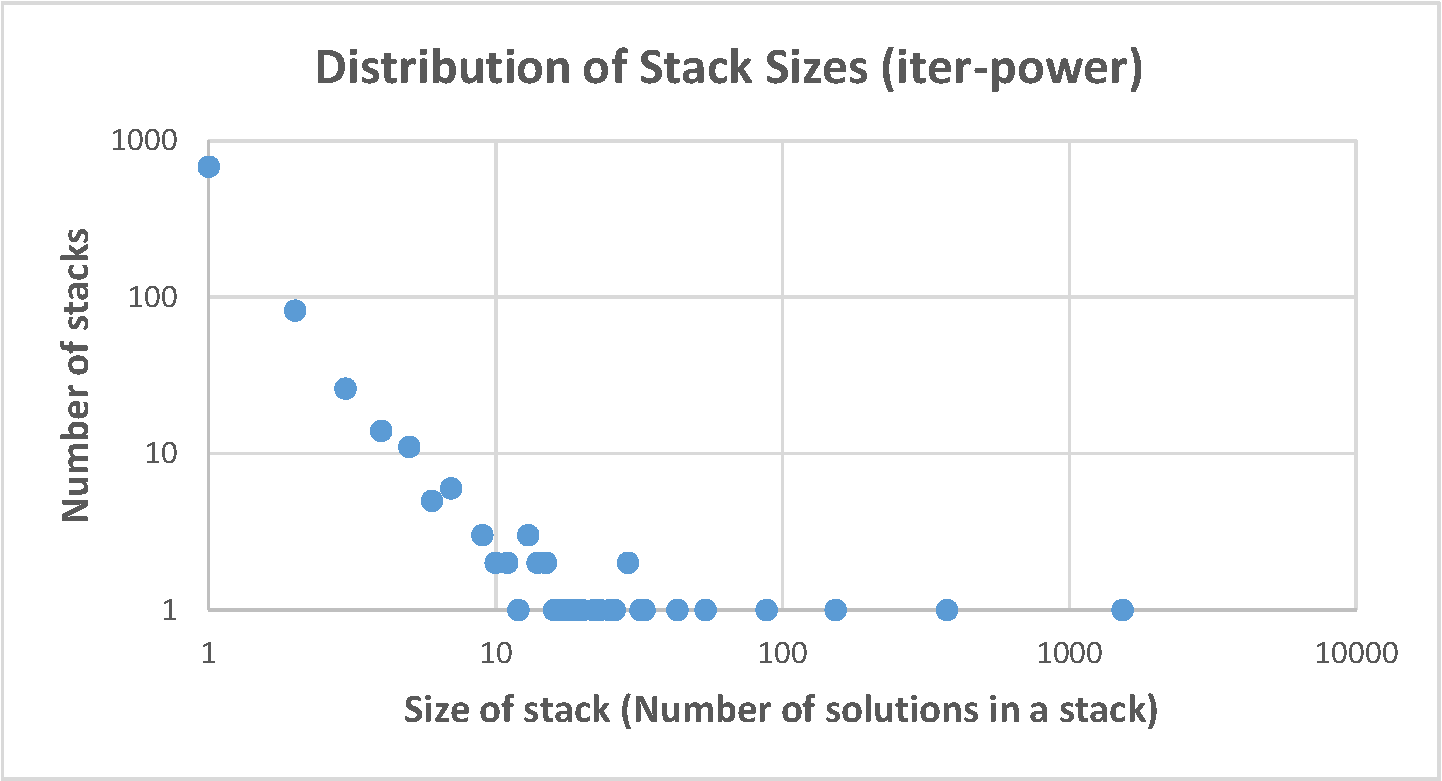
\includegraphics[scale=0.30]{Body/figures/overcode/stacksdistr-iter-power}
&
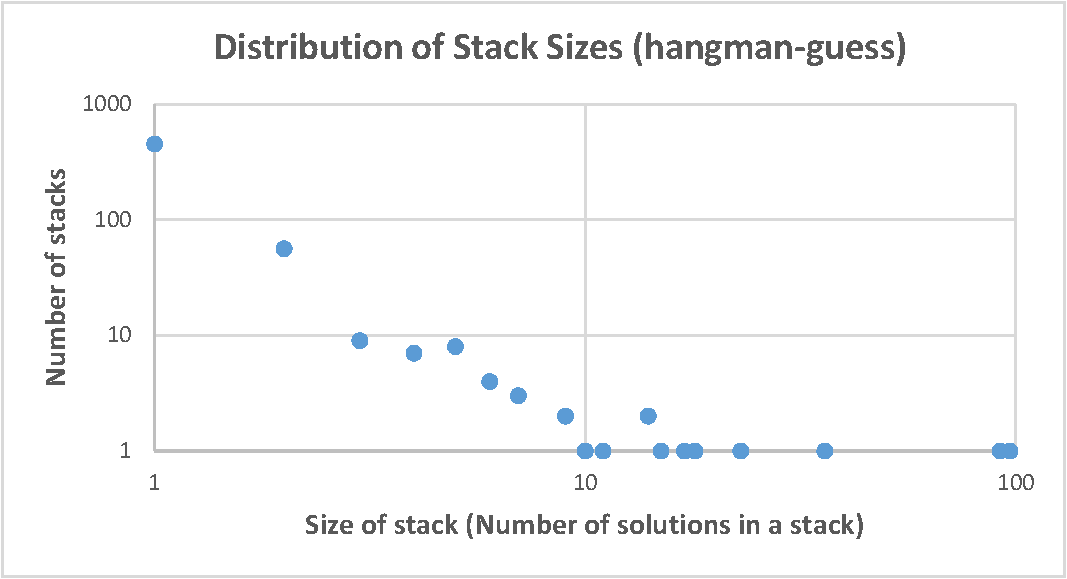
\includegraphics[scale=0.405]{Body/figures/overcode/stacksdistr-hangman}
\end{tabular}
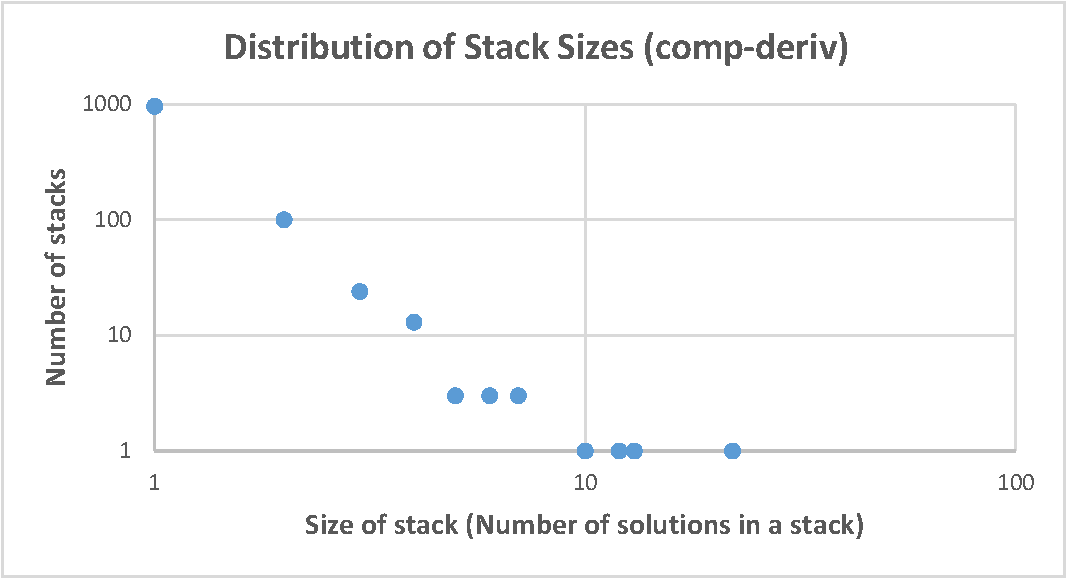
\includegraphics[scale=0.38]{Body/figures/overcode/stacksdistr-comp-deriv}
\caption{The distribution of sizes of the initial stacks generated by our algorithm for each problem, showing a long tail distribution with a few large stacks and a lot of small stacks. Note that the two axes corresponding to the size of stacks and the number of stacks are in logarithmic scale.}
\label{stackdistribution}
\end{figure*}

\begin{figure}[h!]
\begin{tabular}{c}
\\
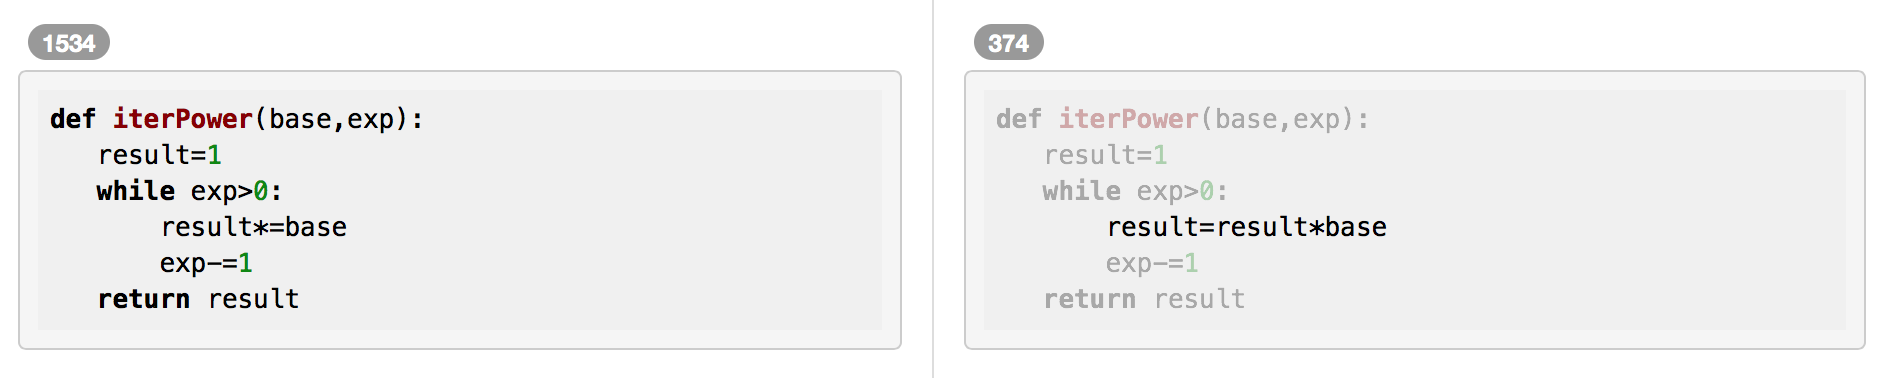
\includegraphics[scale=0.42]{Body/figures/overcode/iterpower-toptwo}
\\ (a) \\ \\
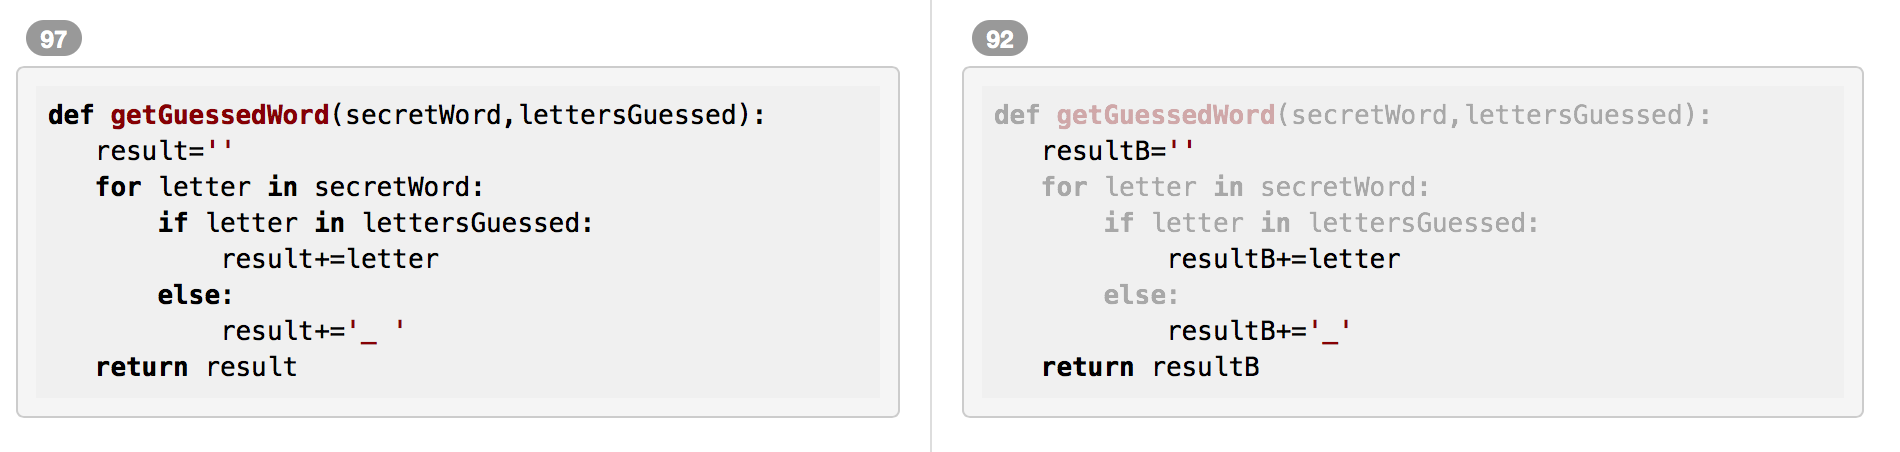
\includegraphics[scale=0.42]{Body/figures/overcode/hangman-toptwo}
\\ (b) \\ \\
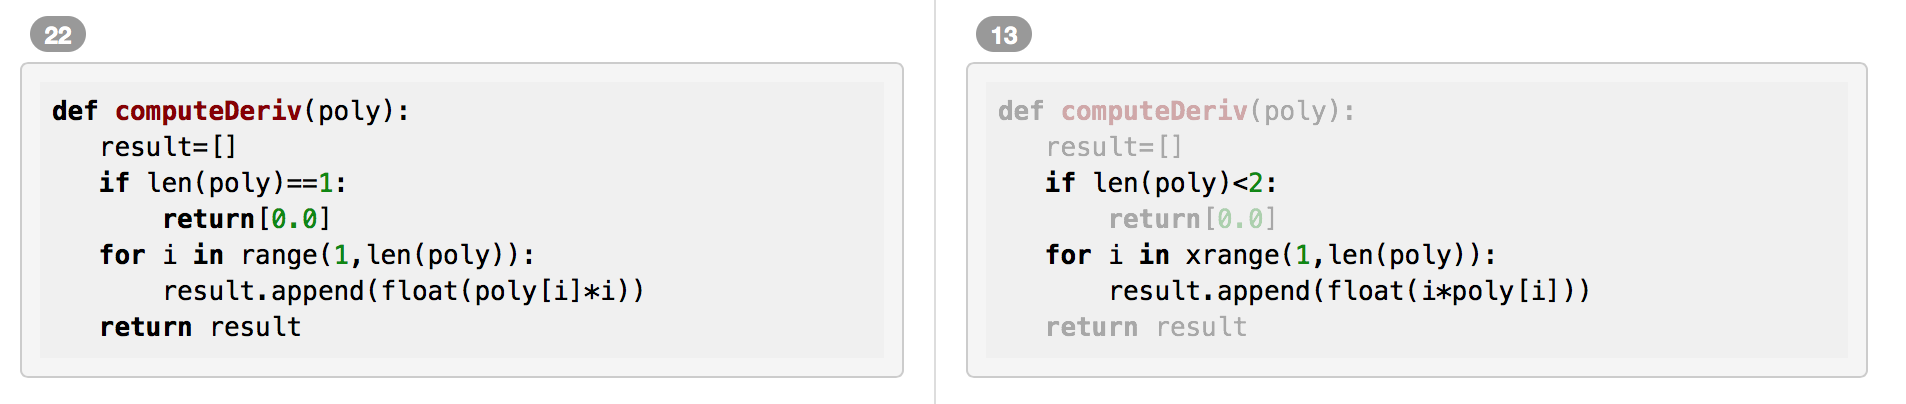
\includegraphics[scale=0.42]{Body/figures/overcode/compderiv-toptwo}
\\ (c) \\
\end{tabular}
\caption{The two largest stacks generated by the OverCode backend algorithm for the (a) \codevar{iterPower}, (b) \codevar{hangman}, and (c)  \codevar{compDeriv} problems.}
\label{toptwostacks}
\end{figure}

{\bf Common Variables} There exists a large variation among the variable names used by students to denote variables that compute the same set of values. The Variable Renaming step of the analysis renames these equivalent variables with the most frequently chosen variable name so that a teacher can easily recognize the role of variables in a given solution. The number of common variables found by the pipeline on the dataset problems is shown in Figure~\ref{backendevaluation} and some examples of these common variable names are shown in Figure~\ref{examplecommonvars}. Figure~\ref{examplecommonvars} also presents the number of times such a variable occurs across the solutions of a given problem, the corresponding variable sequence value on a given test input, and a subset of the original variable names used in the student solutions. 

\begin{figure}
\centering
\scriptsize
\begin{tabular} {|l|r|c|l|}
\hline
{\bf Common} & {\bf Occur} &  \multirow{3}{*}{\bf Sequence of Values} & \multirow{3}{*}{\bf Original Variable Names} \\
{\bf Variable} & {\bf -rence} & & \\
{\bf Name} & {\bf Count} & & \\
 \hline \hline
\multicolumn{4}{|c|}{}\\
\multicolumn{4}{|c|}{\bf iterPower}\\\hline
\codevar{result} & 3081 & [1,5.0,25.0,125.0] & \codevar{result}, \codevar{wynik}, \codevar{out}, \codevar{total}, \codevar{ans}, \codevar{acum}, \codevar{num}, \codevar{mult}, \codevar{output}, $\cdots$\\ \hline
\codevar{exp} & 2744 & [3,2,1,0] & \codevar{exp}, \codevar{iterator}, \codevar{app}, \codevar{ii}, \codevar{num}, \codevar{iterations}, \codevar{times}, \codevar{ctr}, \codevar{b}, $\cdots$\\ \hline
\codevar{exp} & 749 & [3] & \codevar{exp}, \codevar{count}, \codevar{temp}, \codevar{exp3}, \codevar{exp2}, \codevar{exp1}, \codevar{inexp}, \codevar{old\_exp}, $\cdots$\\ \hline
\codevar{i} & 266 & [0,1,2] & \codevar{i}, \codevar{a}, \codevar{count}, \codevar{c}, \codevar{b}, \codevar{iterValue}, \codevar{iter}, \codevar{n}, \codevar{y}, \codevar{inc}, \codevar{x},\codevar{times}, $\cdots$\\ \hline
\multicolumn{4}{|c|}{}\\
\multicolumn{4}{|c|}{\bf hangman}\\\hline
\codevar{letter} & 817 &  [`t',`i',`g',`e',`r'] & \codevar{letter}, \codevar{char}, \codevar{item}, \codevar{i}, \codevar{letS}, \codevar{ch}, \codevar{c}, \codevar{lett}, $\cdots$\\ \hline
\codevar{result} & 291 & [` ',`\_',`\_i',`\_i\_',`\_i\_e',`\_i\_e\_'] & \codevar{result}, \codevar{guessedWord}, \codevar{ans}, \codevar{str1}, \codevar{anss}, \codevar{guessed}, \codevar{string}, $\cdots$\\ \hline
\codevar{i} & 185 & [0,1,2,3,4] & \codevar{i}, \codevar{x}, \codevar{each}, \codevar{b}, \codevar{n}, \codevar{counter}, \codevar{idx}, \codevar{pos} $\cdots$\\ \hline
\codevar{found} & 76 & [0,1,0,1,0] & \codevar{found}, \codevar{n}, \codevar{letterGuessed}, \codevar{contains}, \codevar{k}, \codevar{checker}, \codevar{test}, $\cdots$\\ \hline
\multicolumn{4}{|c|}{}\\
\multicolumn{4}{|c|}{\bf compDeriv}\\ \hline
\codevar{result} & 1186 & [[],[0.0],$\cdots$,[0.0,35.0,9.0,4.0]] & \codevar{result}, \codevar{output}, \codevar{poly\_deriv}, \codevar{res}, \codevar{deriv}, \codevar{resultPoly}, $\cdots$\\ \hline
\codevar{i} & 284 &  [-13.39,0.0,17.5,3.0,1.0] & \codevar{i}, \codevar{each}, \codevar{a}, \codevar{elem}, \codevar{number}, \codevar{value}, \codevar{num}, $\cdots$\\ \hline
\codevar{i} & 261 & [0,1,2,3,4,5] & \codevar{i}, \codevar{power}, \codevar{index}, \codevar{cm}, \codevar{x}, \codevar{count}, \codevar{pwr}, \codevar{counter}, $\cdots$\\ \hline
\codevar{length} & 104 & [5] & \codevar{length}, \codevar{nmax}, \codevar{polyLen}, \codevar{lpoly}, \codevar{lenpoly}, \codevar{z}, \codevar{l}, \codevar{n}, $\cdots$\\ \hline

\end{tabular}
\caption{Some examples of common variables found by our analysis across the problems in the dataset. The table also shows the frequency of occurrence of these variables, the common sequence of values of these variables on a given test case, and a subset of the original variable names used by students.}
\label{examplecommonvars}
\end{figure}

{\bf Collisions in Variable Renaming} The number of Common/Common, Multiple Instances, and Unique/Common collisions discovered and resolved while performing variable renaming is shown in Figure~\ref{collisions}. A large majority of the collisions were Common/Common Collisions. For example, Figure~\ref{examplecommonvars} shows the common variable name \codevar{exp} for two different sequences of values $[3,2,1,0]$ and $[3]$ for the \codevar{iterPower} problem. Similarly, the common variable name \codevar{i} corresponds to sequences $[-13.9, 0.0, 17.5, 3.0, 1.0$ and $[0, 1, 2, 3, 4, 5]$ for the \codevar{compDeriv} problem. There were also a few Multiple Instances collisions and Unique/Common collisions found: 1.5\% for \codevar{iterPower}, 3\% for \codevar{compDeriv}, and 10\% for \codevar{hangman}.

\begin{figure}[htpb]
\centering
\begin{tabular}{|l|r|r|r|r|}
\hline
\multirow{2}{*}{\bf Problem} & {\bf Correct} & {\bf Common/Common} & {\bf Multiple Instances} & {\bf Unique/Common}\\
& {\bf Solutions} & {\bf Collisions } & {\bf Collisions} & {\bf Collisions}\\
\hline \hline
\codevar{iterPower} & 3875 & 1298 & 25 & 32 \\ \hline
\codevar{hangman} & 1118 & 672 & 62 & 49\\ \hline
\codevar{compDeriv} & 1433 & 928 & 21 & 23 \\ \hline
\end{tabular}
\caption{The number of common/common, multiple instances, and unique/common collisions discovered by our algorithm while renaming the variables to common names.}
\label{collisions}
\end{figure}

\section{User Studies}

The goal was to design a system that allows teachers to develop a better understanding of the variation in student solutions, and give feedback that is relevant to more student solutions. Two user studies evaluate our progress in two ways: (1) user interface satisfaction and (2) how many solutions teachers could read and produce feedback on in a fixed amount of time. Reading and providing feedback to thousands of solutions is an unrealistically difficult task for the control condition, so instead of measuring time to finish the entire set of solutions, the experiment measures what subjects could accomplish in a fixed amount of time (15 minutes).

Together, these studies test four hypotheses:
\begin{itemize}
\item \textbf{H1 Interface Satisfaction} Subjects will find OverCode easier to use, more helpful and less overwhelming for browsing thousands of solutions, compared to the baseline. 

\item {\bf H2 Read coverage and speed} Subjects are able to read code that represents more student solutions at a higher rate using OverCode than with the baseline. 

\item {\bf H3 Feedback coverage} Feedback produced when using OverCode is relevant to more student solutions than when feedback is produced using the baseline.

\item {\bf H4 Perceived coverage} Subjects feel that they develop a better high-level view of students' understanding and misconceptions, and provide more relevant feedback using OverCode than with the baseline.

\end{itemize}

\subsection{User Study 1: Writing a Class Forum Post}

The first study was a 12-person within-subjects evaluation of interface satisfaction when using OverCode for a realistic, relatively unstructured task. Using either OverCode or a baseline interface, subjects browse student solutions to the programming problems in our dataset and then write a class forum post on the good and bad ways students solved the problem. This study tests the hypothesis about interface satisfaction (\textbf{H1}).

\subsubsection{OverCode and Baseline Interfaces}

The experiment relies on two interfaces, referred to here as OverCode and the baseline. The OverCode interface and backend are described in detail in Section \ref{overcode}. The baseline interface is a single webpage with all student solutions concatenated in a random order into a flat list, as shown in Figure \ref{iterPowerEdXControl}. This design emulates existing methods of reviewing solutions, and aims to draw out differences between browsing stacked and unstacked solutions. This is analogous to the flat interface chosen as a baseline in another study on interfaces for grading clusters of student work published by Basu et al.~\cite{basuDivideAndConquer}. Basu et al. assume that existing options for reviewing solutions are limited to going through solutions one-by-one. This assumption is supported by our pilot studies, interviews with teaching staff, and our own grading experiences. In edX programming MOOCs, teachers are not even provided with an interface for viewing all solutions at once. They can only look at one student solution at a time. If the solutions can be downloaded locally, some teachers may use a search tool like \codevar{grep}. Our baseline allows for search too, through the in-browser \texttt{Find} command. 

Each solutions is rendered with the same syntax highlighting, background color, and borders in the baseline and OverCode interfaces. However, the solutions shown in the baseline are raw, and the solutions shown in OverCode are normalized. In both interfaces, subjects can use standard web-browser features, such as the within-page \texttt{Find} action.


\begin{figure}[h!]
\centering
\begin{tabular}{cc}
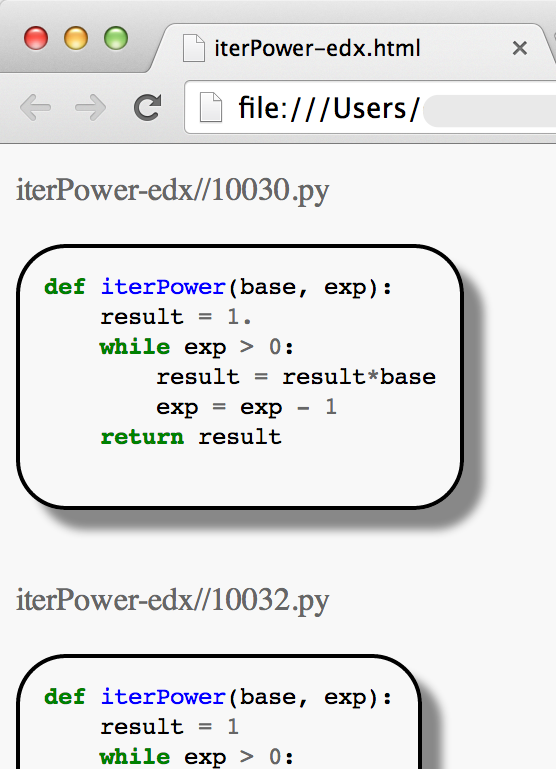
\includegraphics[scale=0.5]{Body/figures/overcode/iterPowerEdXControlStudy1.png} &
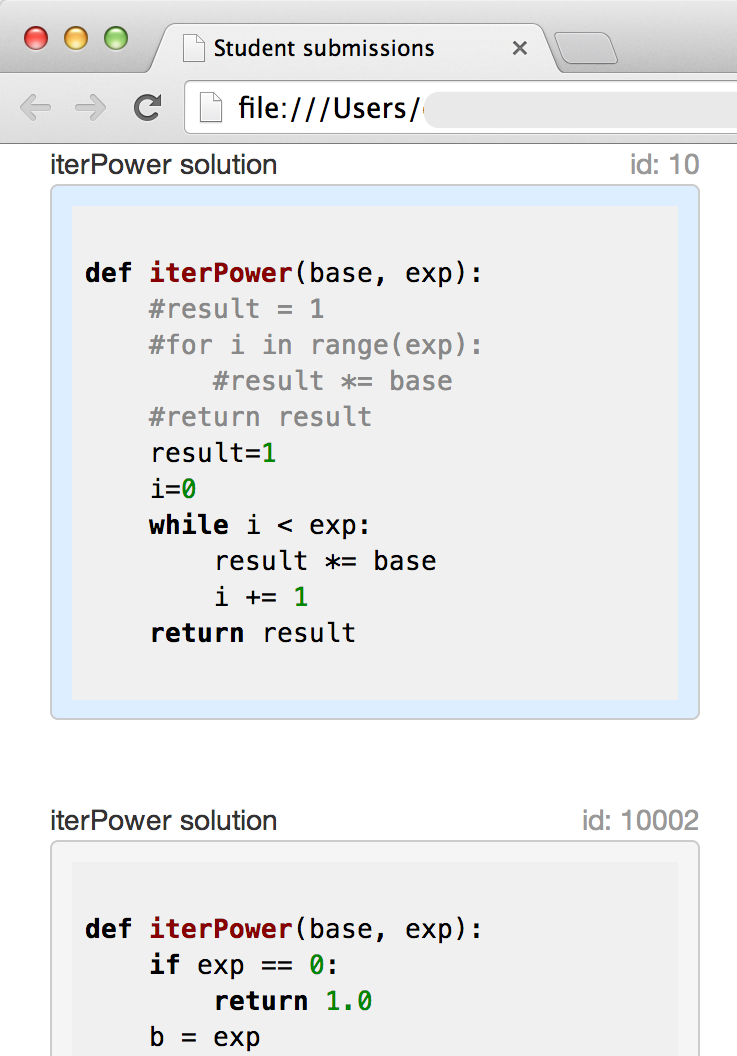
\includegraphics[scale=0.37]{Body/figures/overcode/iterPowerEdXControlStudy2.png} \\
\end{tabular}
\caption{Screenshots of the baseline interface. The appearance changed between the Forum Post study (left) and the Coverage study (right) in order to minimize superficial differences between the baseline and OverCode interfaces. Functionality did not change.}
\label{iterPowerEdXControl}
\end{figure}

\subsubsection{Participants}

Participants joined the study by responding to advertisements sent out to an MIT CSAIL-wide email list as well as past and present staff members of MIT introductory programming courses. These individuals were qualified to participate if they have at least one of the following requirements: (1) taught a computer science course (2) graded Python code before, or (3) significant Python programming experience, making them potential future teaching staff. Participants received \$20 for an hour of their time in the lab. 

Subjects filled out forms about themselves during recruitment and again at the beginning of their one-hour in-lab session. 12 people (7 male) participated, with a mean age of 23.5 ($\sigma = 3.8$). Subjects had a mean 4 years of Python programming experience ($\sigma = 1.8$), and $75\%$ of participants had graded student solutions written in Python before. Half of the participants were graduate students and the other half were undergraduates.

\subsubsection{Apparatus}

Subjects used laptops running MacOS and Linux with screen sizes ranging from 12.5 to 15.6 inches, and viewed the OverCode and baseline interfaces in either Safari or Chrome. Data was recorded with Google Docs and Google Forms filled out by participants.

\subsubsection{Conditions}

Subjects performed the main task of browsing solutions and writing a class forum post twice, once in each interface condition, focusing on one of the three problems in our dataset (Section \ref{dataset}) each time. For each participant, the third remaining problem was used during training, to reduce learning effects when performing the two main tasks. The pairing and ordering of interface and problem conditions were fully counterbalanced, resulting in 12 total conditions. The twelve participants were randomly assigned to one of the 12 conditions, such that all conditions were tested.

\subsubsection{Procedure}

{\bf Prompt} The experimenter began by reading the following prompt, to give the participant context for the tasks they would be performing:

\begin{quote}

We want to help TAs [teaching assistants] give feedback to students in programming classes at scale. For each of three problems, we have a large set of students' submissions ($> 1000$). 

All the submissions are correct, in terms of input and output behavior. We're going to ask you to browse the submissions and produce feedback for students in the class. You'll do this primarily in the form of a class forum post.
\end{quote}

To make the task more concrete, participants reviewed an example\footnote{Our example was drawn from the blog ``Practice Python: 30-minute weekly Python exercises for beginners,'' posted on Thursday, April 24, 2014, and titled ``SOLUTION Exercise 11: Check Primality and Functions.'' (\url{http://practicepython.blogspot.com})} of a class forum post that used examples taken from student solutions to explain different strategies for solving a Python problem. For reference, subjects had print-outs of the prompts for each of the three problems in our dataset.

{\bf Training} The subjects already had extensive experience using web browsers, so training for the baseline interface was minimal. Prior to using the OverCode interface, subjects watched a 3-4 minute long training video demonstrating the features of OverCode, familiarized themselves with the interface, and asked questions. The training session focused on the problem that would not be used in the main tasks, in order to avoid learning effects.

{\bf Tasks} Subjects then performed the main tasks twice, once in each interface, focusing on a different programming problem each time. They were given a fixed amount of time to both read solutions and provide feedback, so task completion times were not measured, but instead the quality of their experience in providing feedback to students at scale.

\begin{itemize}
\item {\it Feedback for Students} (15 minutes) Subjects wrote a class forum post on the good and bad ways students solved the problem. The 15-minute period included both browsing and writing time, as subjects were free to paste in code examples and write comments as they browsed the solutions.

\item {\it Autograder Bugs} (2 min) Although the datasets of student solutions were marked as correct by an autograder, there may be holes in the autograder test cases. Some solutions may deviate from the problem prompt, and therefore be considered incorrect by teachers, e.g., recursive solutions to \codevar{iterPower} when its prompt explicitly calls for an iterative solution. As a secondary task, subjects wrote down any bugs in the autograder they came across while browsing solutions. This was often performed concurrently with the primary task by the subject.
\end{itemize}
{\bf Surveys} Subjects filled out a post-interface condition survey about their experience using the interface. This was a short-answer survey, where they wrote about what they liked, what they did not like, and what they would like to see in a future version of the interface. At the end of the study, subjects rated agreement (on a 7-point Likert scale) with statements about their satisfaction with each interface.

\subsubsection{Results}
Figure~\ref{study1Likert} shows that, compared to the control interface, subjects find OverCode less overwhelming, easier to use, and more helpful for getting a sense of students' understanding. After using both interfaces to view thousands of solutions, subjects found OverCode easier to use ($W=52, Z=2.41, p<0.05, r=0.70$) and less overwhelming ($W=0, Z=-2.86, p<0.005, r=0.83$) than the baseline interface. Finally, participants felt that OverCode ``helped me get a better sense of my students' understanding'' than the baseline did ($W=66, Z=3.04, p<0.001, r=0.88$). These differences are statistically significant, as computed by the Wilcoxon Signed Rank test with pairing users' ratings of each interface. This supports \textbf{H1}, the hypothesis on interface satisfaction.

\begin{figure}
\centering
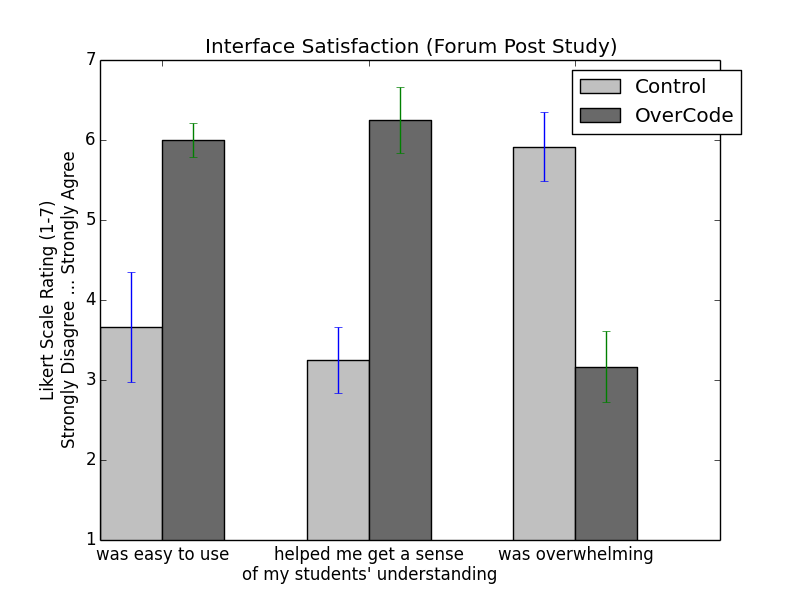
\includegraphics[scale=0.5]{Body/figures/overcode/study1Likert.png}
\caption{{\bf H1: Interface satisfaction} Mean Likert scale ratings (with standard error) for OverCode and baseline interfaces, after subjects used both to perform the forum post writing task.}
\label{study1Likert}
\end{figure}


From the surveys conducted after subjects completed each interface condition, subjects found stacking and the ability to rewrite code to be useful and enjoyable features of OverCode:
\begin{itemize}
\item {\it Stacking is an awesome feature. Rewrite tool is fantastic. Done feature is very rewarding--feels much less overwhelming. "Lines that appear in x submissions" also awesome.}

\item {\it Really liked the clever approach for variable normalization. Also liked the fact that stacks showed numbers, so I'd know I'm focusing on the highest-impact submissions. Impressed by the rewrite ability... it cut down on work so much!}

\item {\it I liked having solutions collapsed (not having to deal with variable names, etc), and having rules to allow me to collapse even further. This made it easy to see the ``plurality'' of solutions right away; I spent most of the time looking at the solutions that only had a few instances.}
\end{itemize}

When asked for suggestions, participants gave many suggestions on stacks, filtering, and rewrite rules, such as:
\begin{itemize}
\item Enable the teacher to change the main stack that is being compared against the others.
\item Suggest possible rewrite rules, based on what the teacher has already written, and will not affect the answers on the test case.
\item Create a filter that shows all stacks that do {\it not} have a particular statement.
\end{itemize}

For both the OverCode and baseline interfaces, the feedback generated about \codevar{iterPower}, \codevar{hangman}, and \codevar{compDeriv} solutions fell into several common themes. One kind of feedback suggested new language features, such as using \codevar{*=} or the keyword \codevar{in}. Another theme identified inefficient, redundant, and convoluted control flow, such as repeated statements and unnecessary statements and variables. It was not always clear what the misconception was, though, as one participant wrote, \textit{``The double iterator solution surely shows some lack of grasp of power of for loop, or range, or something.''} Participant feedback included comments on the relative goodness of different correct solutions in the dataset. This was a more holistic look at student solutions as they varied along the dimensions of conciseness, clarity, and efficiency previously described.

Study participants found both noteworthy correct solutions and solutions they considered incorrect, despite passing the autograder. One participant learned a new Python function, \codevar{enumerate}, while looking at a solution that used it. The participant wrote, \textit{``Cool, but uncalled for. I had to look it up :]. Use, but with comment.''} Participants also found recursive \codevar{iterPower} and \codevar{hangman} solutions, which they found noteworthy. For what should have been an iterative \codevar{iterPower} function, the fact that this recursive solution was considered correct by the autograder was considered an autograder bug by some participants. Using the built-in Python exponentiation operator \codevar{**} was also considered correct by the autograder, even though it subverted the point of the assignment. It was also noted as an autograder bug by some participants who found it.

\subsection{User Study 2: Coverage}

A second 12-person study was designed, similar in structure to the forum post study, but focused on measuring the coverage achieved by subjects in a fixed amount of time (15 minutes) when browsing and producing feedback on a large number of student solutions. The task in the second study was more constrained than the first. Instead of writing a freeform post, subjects identified the five most frequent strategies used by students and rated their confidence that these strategies occurred frequently in the student solutions. These changes to the task enabled us to measure coverage in terms of solutions read, the relevance of written feedback and the perceived coverage of the subject. This study tests the remaining hypotheses on read coverage and speed ({\bf H2}), feedback coverage ({\bf H3}) and perceived coverage ({\bf H4}).

The OverCode and baseline interfaces changed slightly prior to running the second study. Figure \ref{iterPowerEdXControl} shows the baseline changes that reduce the differences between the rendering of solutions in the baseline and OverCode interfaces. The OverCode interface was changed to show identifiers next to every stack and solutions so that subjects could provide it when asked.

\subsubsection{Participants, Apparatus, Conditions}

The coverage study shared the same methods for recruiting participants, apparatus and conditions as the forum post study. 12 new participants (11 male) participated in the second study (mean age = 25.4, $\sigma = 6.9$). Across those 12 participants, the mean years of Python programming experience was 4.9 ($\sigma = 3.0$) and 9 of them had previously graded code (5 had graded Python code). Subjects included 5 graduate students, 6 undergraduates, and 1 independent computer software professional.


\subsubsection{Procedure}
{\bf Prompt} In the coverage study, the prompt was similar to the one used in the forum post study, explaining that the subjects would be tackling the problem of producing feedback for students at scale. The language was modified to shift the focus towards finding frequent strategies used by students, rather than any example of good or bad code used by a student.%\todo{find prompt and put it in here}

{\bf Training} As before, subjects watched a training video and given time to practice using OverCode features prior to their trial in the OverCode condition.

{\bf Task} The coverage study task consisted of a more constrained feedback task. Given 15 minutes with either the OverCode or baseline interface, subjects filled out a table, identifying the five most frequent strategies used by students to solve the problem. For each strategy they identified, they filled in the following fields in the table:
\begin{itemize}
\item A code example taken from the solution or stack.
\item The identifier of the solution or stack.
\item A short (one sentence) annotation of what was good or bad about the strategy.
\item Their confidence, on a scale of 1-7, that the strategy frequently occurred in the student solutions.
\end{itemize}
Importantly, subjects marked solutions or stacks as \emph{read} by clicking on them after they had processed them, even if they did not choose them as representative strategies. We combined this data with logs of subject actions in the interface to quantify read coverage.

{\bf Surveys} Although we measured interface satisfaction for a realistic task in the forum post study, we also measured interface satisfaction through surveys for this more constrained, coverage-focused task. Subjects filled out a post-interface condition survey in which they rated agreement (on a 7-point Likert scale) with positive and negative adjectives about their experience using the interface, and reflected on task difficulty. At the end of the study, subjects rated their agreement with statements about the usefulness of specific features of both the OverCode and baseline interfaces, and responded to the same interface satisfaction 7-point Likert scale statements used in the first study.

\subsubsection{Results} \label{coverageResults}
\begin{figure*}[b!]
\begin{tabular}{c | c}
\begin{minipage}{.5\linewidth}
\centering
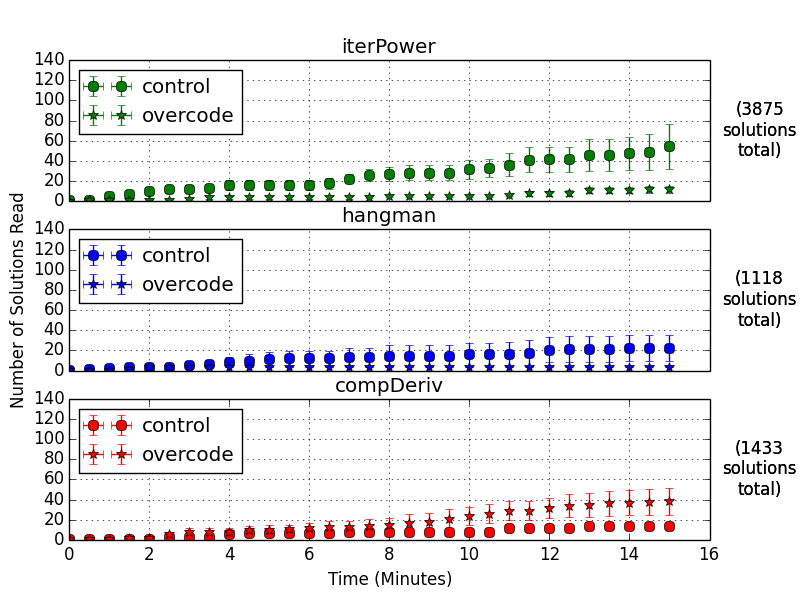
\includegraphics[width=\linewidth]{Body/figures/overcode/prettyReadCoverage.png}
\end{minipage}
&
\begin{minipage}{.5\linewidth}
\centering
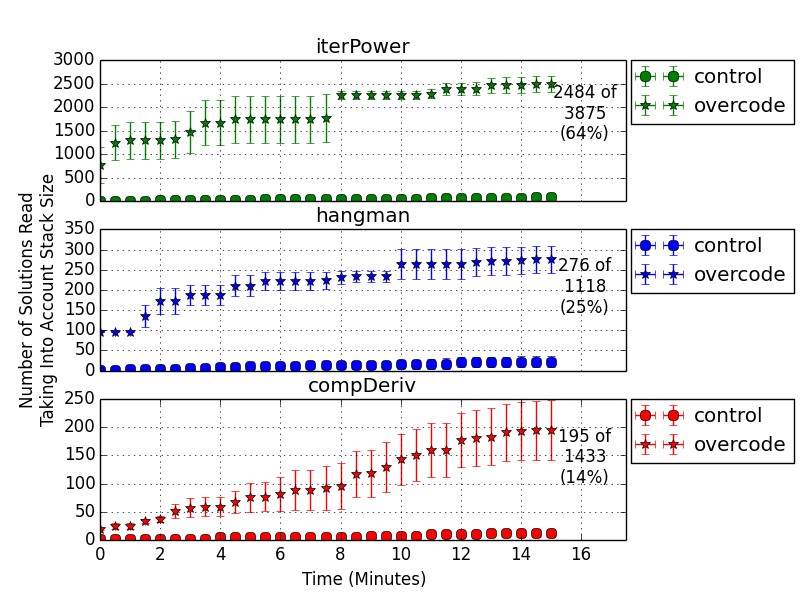
\includegraphics[width=\linewidth]{Body/figures/overcode/prettyPercentCoverage.png}
\end{minipage}
\\
(a) & (b)
\end{tabular}
\caption{In (a), we plot the mean number of platonic solutions read in OverCode over time versus the number of raw solutions read in the baseline interface over time while performing the 15-minute Coverage Study task. In (b), we replace the mean number of platonic solutions with the mean number of solutions, i.e., the stack size, they represent. These are shown for each of the three problems in the dataset.}
\label{readCoverage}
\end{figure*}

{\bf H2: Read coverage and speed} Figure \ref{readCoverage} shows that subjects reading platonic \texttt{iterPower}, \texttt{hangman}, and \texttt{compDeriv} solutions in the OverCode interface covered the equivalent of 64\%, 25\%, and 14\% of all student solutions to those problems (Mann--Whitney U = 16, n1 = n2 = 4, p<0.05). Subjects read through more raw solutions than platonic solutions to the simplest problems, i.e., \texttt{iterPower} and \texttt{hangman}, but when problem difficulty increased, i.e., \texttt{compDeriv}, subjects read through the platonic solutions in the OverCode interface faster than raw solutions. This supports the H2 hypothesis.

%This hypothesis is supported by our measurements of read coverage from this study. For each problem, subjects were able to view more normalized and stacked solutions by the end of the 15-minute-long main task using OverCode than raw solutions when using the baseline interface (Mann--Whitney U = 16, n1 = n2 = 4, p<0.05). Figure \ref{readCoverage} shows the mean number of solutions read over time for each interface and each problem in our dataset. The curves show that subjects were able to read code that represented more raw solutions at a higher rate due to the stacking of similar solutions.

{\bf H3: Feedback coverage} Each subject reported on the five most frequent strategies in a set of solutions, by copying both a code example and the identifier of the solution (baseline) or stack (OverCode) that it came from. We define \emph{feedback coverage} as the number of students for which the quoted code is relevant, in the sense that they wrote the same lines of code, ignoring differences in whitespace or variable names. We computed the coverage for each example using the following process:
\begin{itemize}
\item Reduce the quoted code down to only the lines referred to in the annotation. Often, the annotation would focus on a specific feature of the quoted code, which sometimes included additional lines unrelated to the written feedback. For example, comments about iterating over a range function, while also quoting the contents of the for loop. This step meant we would be calculating the coverage of a more general, smaller set of lines.

\item Find the source stack that the quoted code comes from. This is trivial in the OverCode condition, where the subject wrote down a stack ID. In the baseline condition, the subject wrote down the solution ID. During post-study analysis, the authors determined which stack the solution is in, as determined by the OverCode analysis pipeline.

\item Find the normalized version of each quoted line. The quoted lines of code may be raw code if they come from the baseline condition. By comparing the quoted code with the normalized code of its source stack, we found the normalized version of each line, with variable names and whitespace normalized.

\item Find the raw solutions that include the set of normalized lines, using a map from stacks to raw solutions provided by the backend pipeline.
\end{itemize}

\begin{figure}[b!]
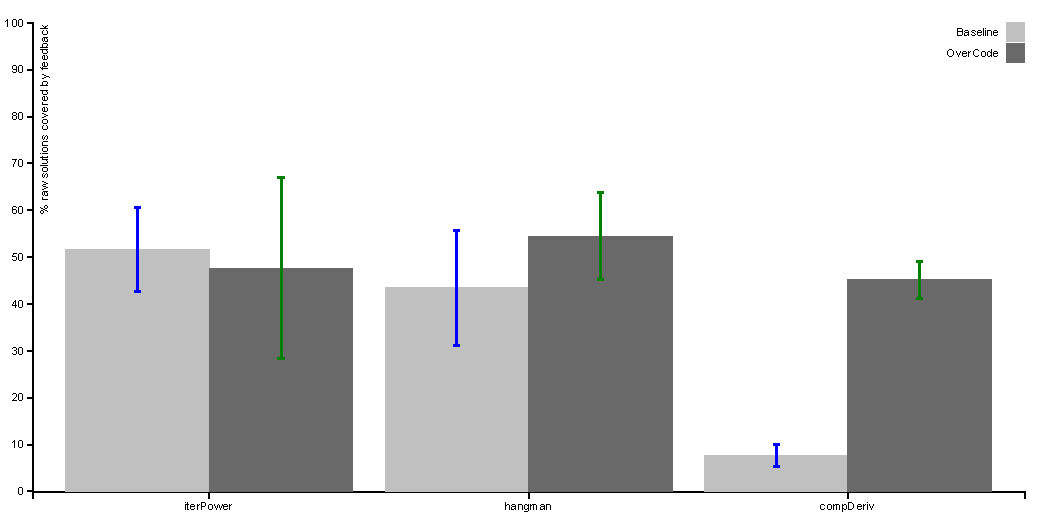
\includegraphics[width=0.6\paperwidth]{Body/figures/overcode/feedbackCoverage.pdf}
\caption{Mean feedback coverage, i.e., the percentage of raw solutions covered, per trial during the coverage study for each problem, in the OverCode and baseline interfaces.}
\label{aveCoveragePerPost}
\end{figure}
%\todo{DNHT: what are the error bars?}

Figure \ref{aveCoveragePerPost} shows the mean coverage of a set of feedback produced by a single subject, across problems and interface conditions. The feedback coverage is shown as the mean percentage of raw solutions for which the feedback was relevant. When giving feedback on the \codevar{iterPower} and \codevar{hangman} problems, there was not a statistically significant difference in the feedback coverage between interface conditions. However, on \codevar{compDeriv}, the problem with the most complex solutions, subjects using OverCode achieved significantly more coverage of student solutions than when using the baseline interface (Mann--Whitney U = 0, n1 = n2 = 4, p< 0.05).

\begin{figure*}[t!]
\begin{tabular}{c | c}
\begin{minipage}{.5\linewidth}
\centering
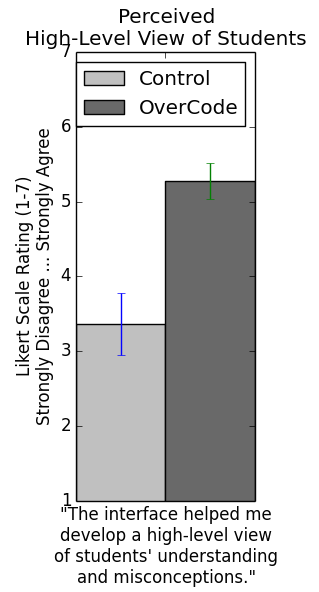
\includegraphics[scale=0.5]{Body/figures/overcode/highLevelViewStudy2.png}
\end{minipage}
&
\begin{minipage}{.5\linewidth}
\centering
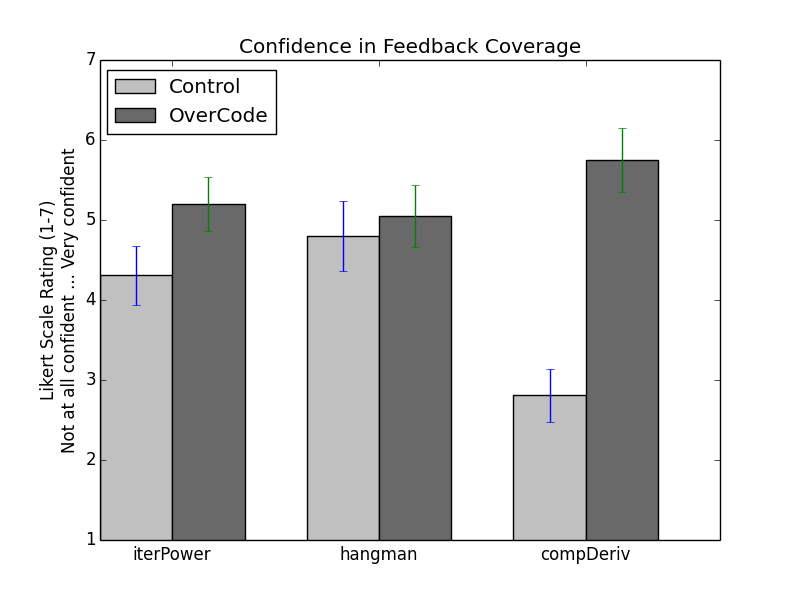
\includegraphics[width=\linewidth]{Body/figures/overcode/coverageConfidence.png}
\end{minipage}
\\
(a) & (b)
\end{tabular}
\caption{Mean rating with standard error for (a) post-condition perception of coverage (excluding one participant) and (b) confidence ratings that identified strategies were frequently used (1-7 scale).}
\label{perceivedCoverage}
\end{figure*}

{\bf H4: Perceived coverage} After using each interface, we asked participants how strongly they agreed with the statement `This interface helped me develop a high-level view of students' understanding and misconceptions,' which quotes the first part of our third hypothesis. Participants agreed with this statement after using OverCode significantly more than when using the baseline interface ($W=63, Z=2.70, p<0.01, r=0.81$). Statistical significance was computed using the Wilcoxon Signed Rank test, pairing users' ratings of each interface. The analysis was done for only 11 participants because the data of one participant was lost. The mean rating with standard error for the responses is shown in Figure~\ref{perceivedCoverage}(a). 

For each strategy identified by subjects, we asked them to rate their confidence, on a scale of 1-7, that the strategy was frequently used by students in the dataset. Mean confidence ratings on a per-problem basis are shown in Figure \ref{perceivedCoverage}(b). We found that for \codevar{compDeriv}, subjects using OverCode felt significantly more confident that their annotations were relevant to many students, compared to the baseline (Mann--Whitney $U=260.5, n_{1}=18, n_{2}=16, p<0.0001$).
 
{\bf H1: Interface satisfaction} Interface satisfaction was measured through multiple surveys, (1) immediately after using each interface and (2) after using both interfaces. Statistical significance was computed using the Wilcoxon Signed Rank test, pairing users' ratings of each interface. 

Immediately after finishing the assigned tasks with an interface, participants rated their agreement with statements about the appropriateness of various adjectives to describe the interface they just used, on a 7-point Likert scale. While participants found the baseline to be significantly more simple ($W=2.5, Z=-2.60, p<0.01, r=0.78$), they found OverCode to be significantly more flexible ($W=45, Z=2.84, p<0.005, r=0.86$), less tedious ($W=3.5, Z=-2.41, p<0.05, r=0.73$), more interesting ($W=66, Z=2.96, p<0.001, r=0.89$), and more enjoyable ($W=45, Z=2.83, p<0.005, r=0.85$). The analysis was done for only 11 participants because the data of one participant was lost. The mean ratings (with standard error) for the responses are shown in Figure~\ref{studyLikert1_onPop2}. 

After the completion of the Coverage Study, participants rated their agreement with statements about each interface on a 7-point Likert scale. After using both interfaces to view thousands of solutions, there were no significant differences between how overwhelming or easy to use each interface was. However, participants did feel that OverCode ``helped me get a sense of my students' understanding'' more than the baseline ($W=62.5, Z=-2.69, p<0.01, r=0.78$). The mean ratings for the responses are shown in Figure~\ref{studyLikert1_onPop2}, as well as the standard error.

\begin{figure}
\centering
\begin{tabular}{c c}
\begin{minipage}{.6\linewidth}
\centering
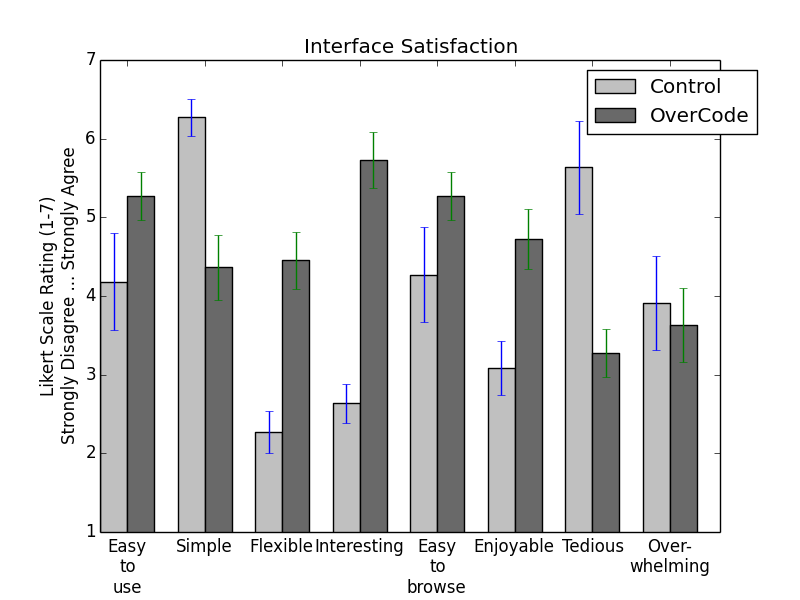
\includegraphics[scale=0.35]{Body/figures/overcode/study2Likert.png}
\end{minipage}
&
\begin{minipage}{.4\linewidth}
\centering
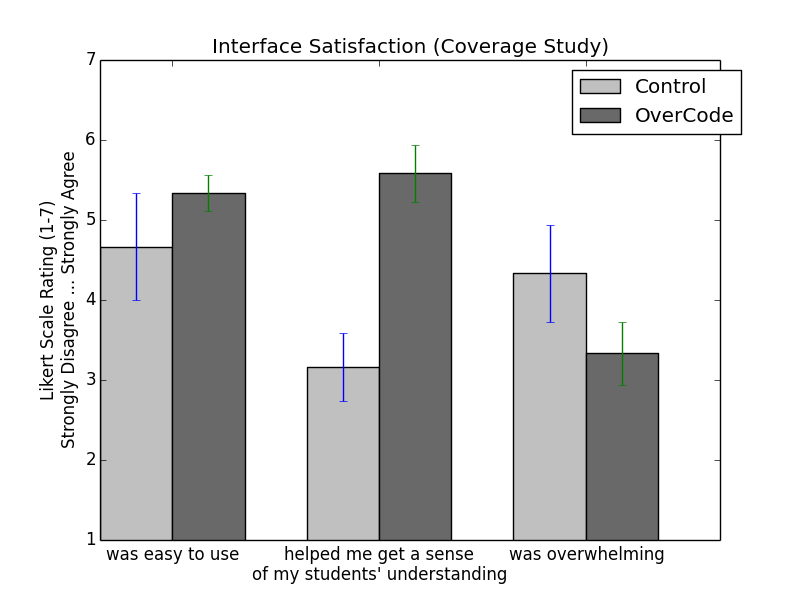
\includegraphics[scale=0.30]{Body/figures/overcode/study1Likert_onPop2.png}
\end{minipage}
\\
(a) & (b)
\end{tabular}
\caption{{\bf H1: Interface satisfaction} Mean Likert scale ratings (with standard error) for  OverCode and baseline, (a) immediately after using the interface for the Coverage Study task, and (b) after using both interfaces.}
\label{studyLikert1_onPop2}
\end{figure}

{\bf Usage and Usefulness of Interface Features} In the second part of the post-study survey, participants rated their agreement with statements about the helpfulness of various interface features on a 7-point Likert scale. There were only two features to ask about in the baseline interface, in-browser find and viewing raw solutions. Statements about these baseline features were mixed in with statements about OverCode features. The OverCode feature of stacking equivalent solutions was found more helpful than the baseline features of in-browser find ($W=41, Z=2.07, p<0.05, r=0.60$) and viewing raw student solutions, comments included ($W=45, Z=2.87, p<0.005, r=0.83$). Subjects found both the OverCode feature of variable renaming and previewing rewrite rules significantly more helpful than seeing raw student code ($W=65.5, Z=2.09, p<0.05, r=0.61$ and $W=56.5, Z=2.14, p<0.05, r=0.62$, respectively). The mean ratings for the features are shown in Figure~\ref{featureHelpfulness}.

\begin{figure}
\centering
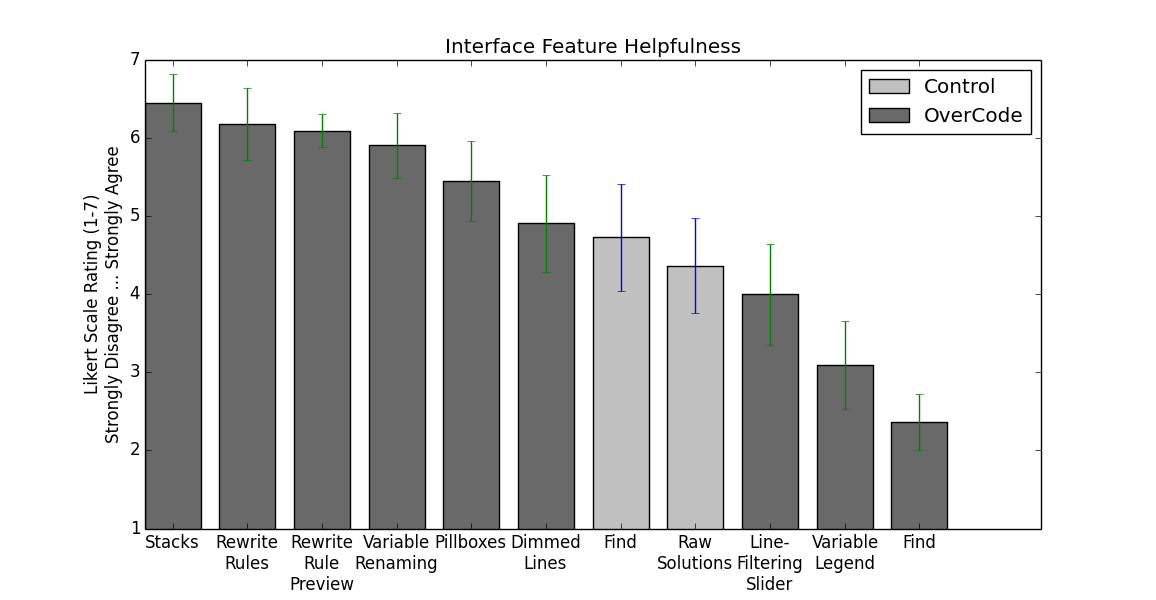
\includegraphics[scale=0.5]{Body/figures/overcode/featureHelpfulness.png}
\caption{Mean Likert scale ratings (with standard error) for the usefulness of features of OverCode and baseline. {\it Find} refers to the find function within the web browser. {\it Find} appears twice in this figure because users rated its usefulness for each condition.}
\label{featureHelpfulness}
\end{figure}

In addition to logging \codevar{read} events, we also recorded usage of interface features, such as creating rewrite rules and filtering stacks. A common usage strategy was to read through the stacks linearly and mark them as \codevar{read}, starting with the largest reference stack, then rewrite trivial variations in expressions to merge smaller behaviorally equivalent stacks into the largest stack. Stack filtering (Figure~\ref{linefilter}) was sometimes used to review solutions that contained a particularly conspicuous line, e.g., a recursive call to solve \codevar{iterPower} or an extremely long expression. Subjects rarely used the filter panel frequency slider (Figure~\ref{linefilter}a) and the variable legend (Figure~\ref{afterrewrite}b).

All subjects wrote at least two rewrite rules, often causing stacks to merge that only differed in some trivial way, like reordering operands in multiplication statements, e.g., \codevar{result = result*base} vs. \codevar{result = base*result}. Some rewrite rules merged Python expressions that behaved similarly but differed in their verbosity, e.g., \codevar{for i in range(0, exp)} vs. \codevar{for i in range(exp)}. These variations may be considered noteworthy or trivial by different teachers.

\section{Discussion}

A three-part evaluation of the OverCode backend and user interface demonstrates its usability and usefulness in a realistic teaching scenario. Given that the datasets are drawn from the first three weeks of an introductory Python programming course, the evaluation is limited to single functions, whose most common solutions were less than ten lines long. Some of these functions were recursive, while most were iterative. Variables were generally limited to booleans, integers, strings, and lists of these basic data types. All solutions had already passed the autograder tests, and study participants still found solutions that suggested student misconceptions or knowledge gaps. Future work will address more complex algorithms and data types.

\subsubsection{Read coverage}
Subjects covered more student solutions when reading solutions in the OverCode interface (H1, read coverage). This is expected, because in OverCode each read stack represented tens or hundreds of raw solutions, while there was only a 1-to-1 mapping between read solutions and raw solutions in the baseline condition. The OverCode backend produces platonic solutions that represent many raw solutions, reducing the cognitive load of mentally processing all the raw solutions, including their variation in formatting and variable naming.

Figure \ref{readCoverage}(a) shows that in some cases, subjects read nearly as many (\codevar{hangman}) or more (\codevar{iterPower}) function definitions in the baseline as in OverCode. In the case of \codevar{iterPower}, the raw solutions are repetitive because of the simplicity of the problem and the relatively small amounts of variation demonstrated by student solutions. This can explain the ability of subjects to move quickly through the set of solutions, reading as many as 90 solutions in 15 minutes.

Figure \ref{readCoverage}(b) shows the effective number of raw solutions read, when accounting for the number of solutions represented by each platonic solution read in the OverCode condition. In the case of \codevar{iterPower}, subjects can say they have effectively read more than 30\% of student solutions after reading the first stack. A similar statement can be made for \codevar{hangman}, where the largest stack includes roughly 10\% of solutions. In the case of \codevar{compDeriv}, the small size of its largest stack (22 out of 1433 raw solutions) means that the curve is less steep, but the use of rewrite rules (avg. 4.5 rules written per \codevar{compDeriv} subject) enabled subjects to cover over 10x the solutions covered by subjects in the baseline condition.

\subsubsection{Feedback coverage}
We also found that subject-written feedback on solutions for the \codevar{compDeriv} problem had significantly higher coverage when produced using OverCode than with the baseline, but that this was not the case for the \codevar{iterPower} and \codevar{hangman} problems. \codevar{compDeriv} was a significantly more complicated problem than both \codevar{iterPower} and \codevar{hangman}, meaning that there was a greater amount of variation between student solutions. This high variation meant that any one piece of feedback might not be relevant to many raw solutions, unless it was produced after viewing the solution space as stacks and creating rewrite rules to simplify the space into larger, more representative stacks. Conversely, the simple nature of \codevar{iterPower} and \codevar{hangman} meant that there was less variation in student solutions. Therefore, regardless of whether the subject was using the OverCode or baseline condition, there was a higher likelihood that they would stumble across a solution that had frequently occurring lines of code, and the feedback coverage for these problems became comparable between the two problems.

\subsubsection{Perceived coverage}
In addition to the actual read and feedback coverage that subjects achieved, an important finding was that (i) subjects felt they had developed a better high-level understanding of student solutions and (ii) subjects stated they felt more confident that identified strategies were frequent issues in the dataset. While a low self-reported confidence score did not necessarily correlate with low feedback coverage, these results suggest that OverCode enables the teacher to gauge the impact that their feedback will have.

%\section{Modifications and Extensions}

%\subsection{Handling Multiple Test Cases}
%For the convenience and speed of adding more solutions without unnecessary repeated computation,

%\subsection{Multiple Test Cases and Efficiency} 
%Since publication, the OverCode pipeline has been modified in several ways. 
%\subsection{Collecting Additional Information per Line}~\label{subsec:morelineinfo}
%, as described in Section~\ref{subsec:grovercodepipeline}.
% is, without being affected a very similar concept, except it is more robust to non-local variations in variable behavior. For example, if the line of code \texttt{for ___ in range(___):}initialization of two common variables 

\subsubsection{Clarity in Variable Renaming}
The modifiers appended to common variables to resolve Common/Common collisions caused some confusion. For example, \texttt{iB} is a legitimate, but odd, variable name. To indicate that the modifier is not something the student wrote themselves, modifiers are now rendered in the interface as numerical subscripts indicating whether they are the second or third or fourth, etc., most frequently occurring common variable with that name across all the solutions in the collection.

\section{GroverCode: OverCode for Grading}\label{sec:grover}

While understanding the contents of thousands of correct student solutions can be helpful in both residential and online contexts, another application of the OverCode pipeline and interface is supporting the hand-grading of introductory Python programming exam solutions, only some of which are correct. Incorrect solutions are defined as those that do not pass at least one test case in the teacher-designed test suite.

Hand-reviewing solutions is necessary because test suites can unfairly penalize some students and award undeserved credit to others. For example, a single typo in an otherwise well-written solution can cause it to fail all the test cases and receive no credit. Conversely, a solution that subverts the purpose of the assignment can still receive credit by returning the expected answer to some or all of the test cases.

For the staff of 6.0001, the residential introductory Python programming course at MIT, this can be one of the most time-consuming and exhausting parts of teaching the course. It can take a full workday for the entire staff of eight to ten teachers to sit in a room and review several hundred student solutions by hand in order to assign a single numerical grade to each solution.

Stacey Terman, in partial fulfilment of her Master's of Engineering, worked with me to extend OverCode to a new domain, i.e., incorrect solutions, and a new task, i.e., grading hundreds of incorrect solutions by hand~\cite{staceythesis}. This new version of OverCode for grading is referred to as GroverCode. GroverCode was iteratively designed and evaluated as a grading tool through two live deployments during the Spring 2016 6.0001 staff exam grading sessions. The following tables, figures, and code samples generated from those deployments are adapted with permission from that thesis.

GroverCode contains two main technical contributions: a modified pipeline that can normalize both correct and incorrect solutions and an interface designed for grading. Just as the original pipeline used variable behavior to normalize variable names, the modified pipeline uses variable behavior and the syntax of statements containing each variable to normalize variable names in solutions that are not correct. This comes from the insight that a variable in an incorrect solution can be semantically equivalent to a variable in a correct solution but still behave differently. It can behave differently due to a bug in a line of code that directly modifies its value or a bug in a line of code that affects the behavior of another variable that it depends on. Since many of the exam solutions are incorrect and do not get clustered together, the new user interface organizes solutions according to their behavior on test cases and compositional similarity to each other, rather than by cluster size.

\subsubsection{User Interface}

The GroverCode interface, shown in Figure~\ref{fig:whole_interface}, has several additions and distinctions from the OverCode interface. As shown in Figure~\ref{fig:correct_and_incorrect_stacks}, both correct solutions and incorrect solutions are displayed, differentiable by their varied background colors and red X next to every failed test. To better explain each test failure, the actual and expected outputs are displayed beneath each solution. The staff iteratively develop a rubric as they grade. Figure~\ref{fig:rubric} is a snapshot of one of these rubrics.

\begin{figure}
\centering
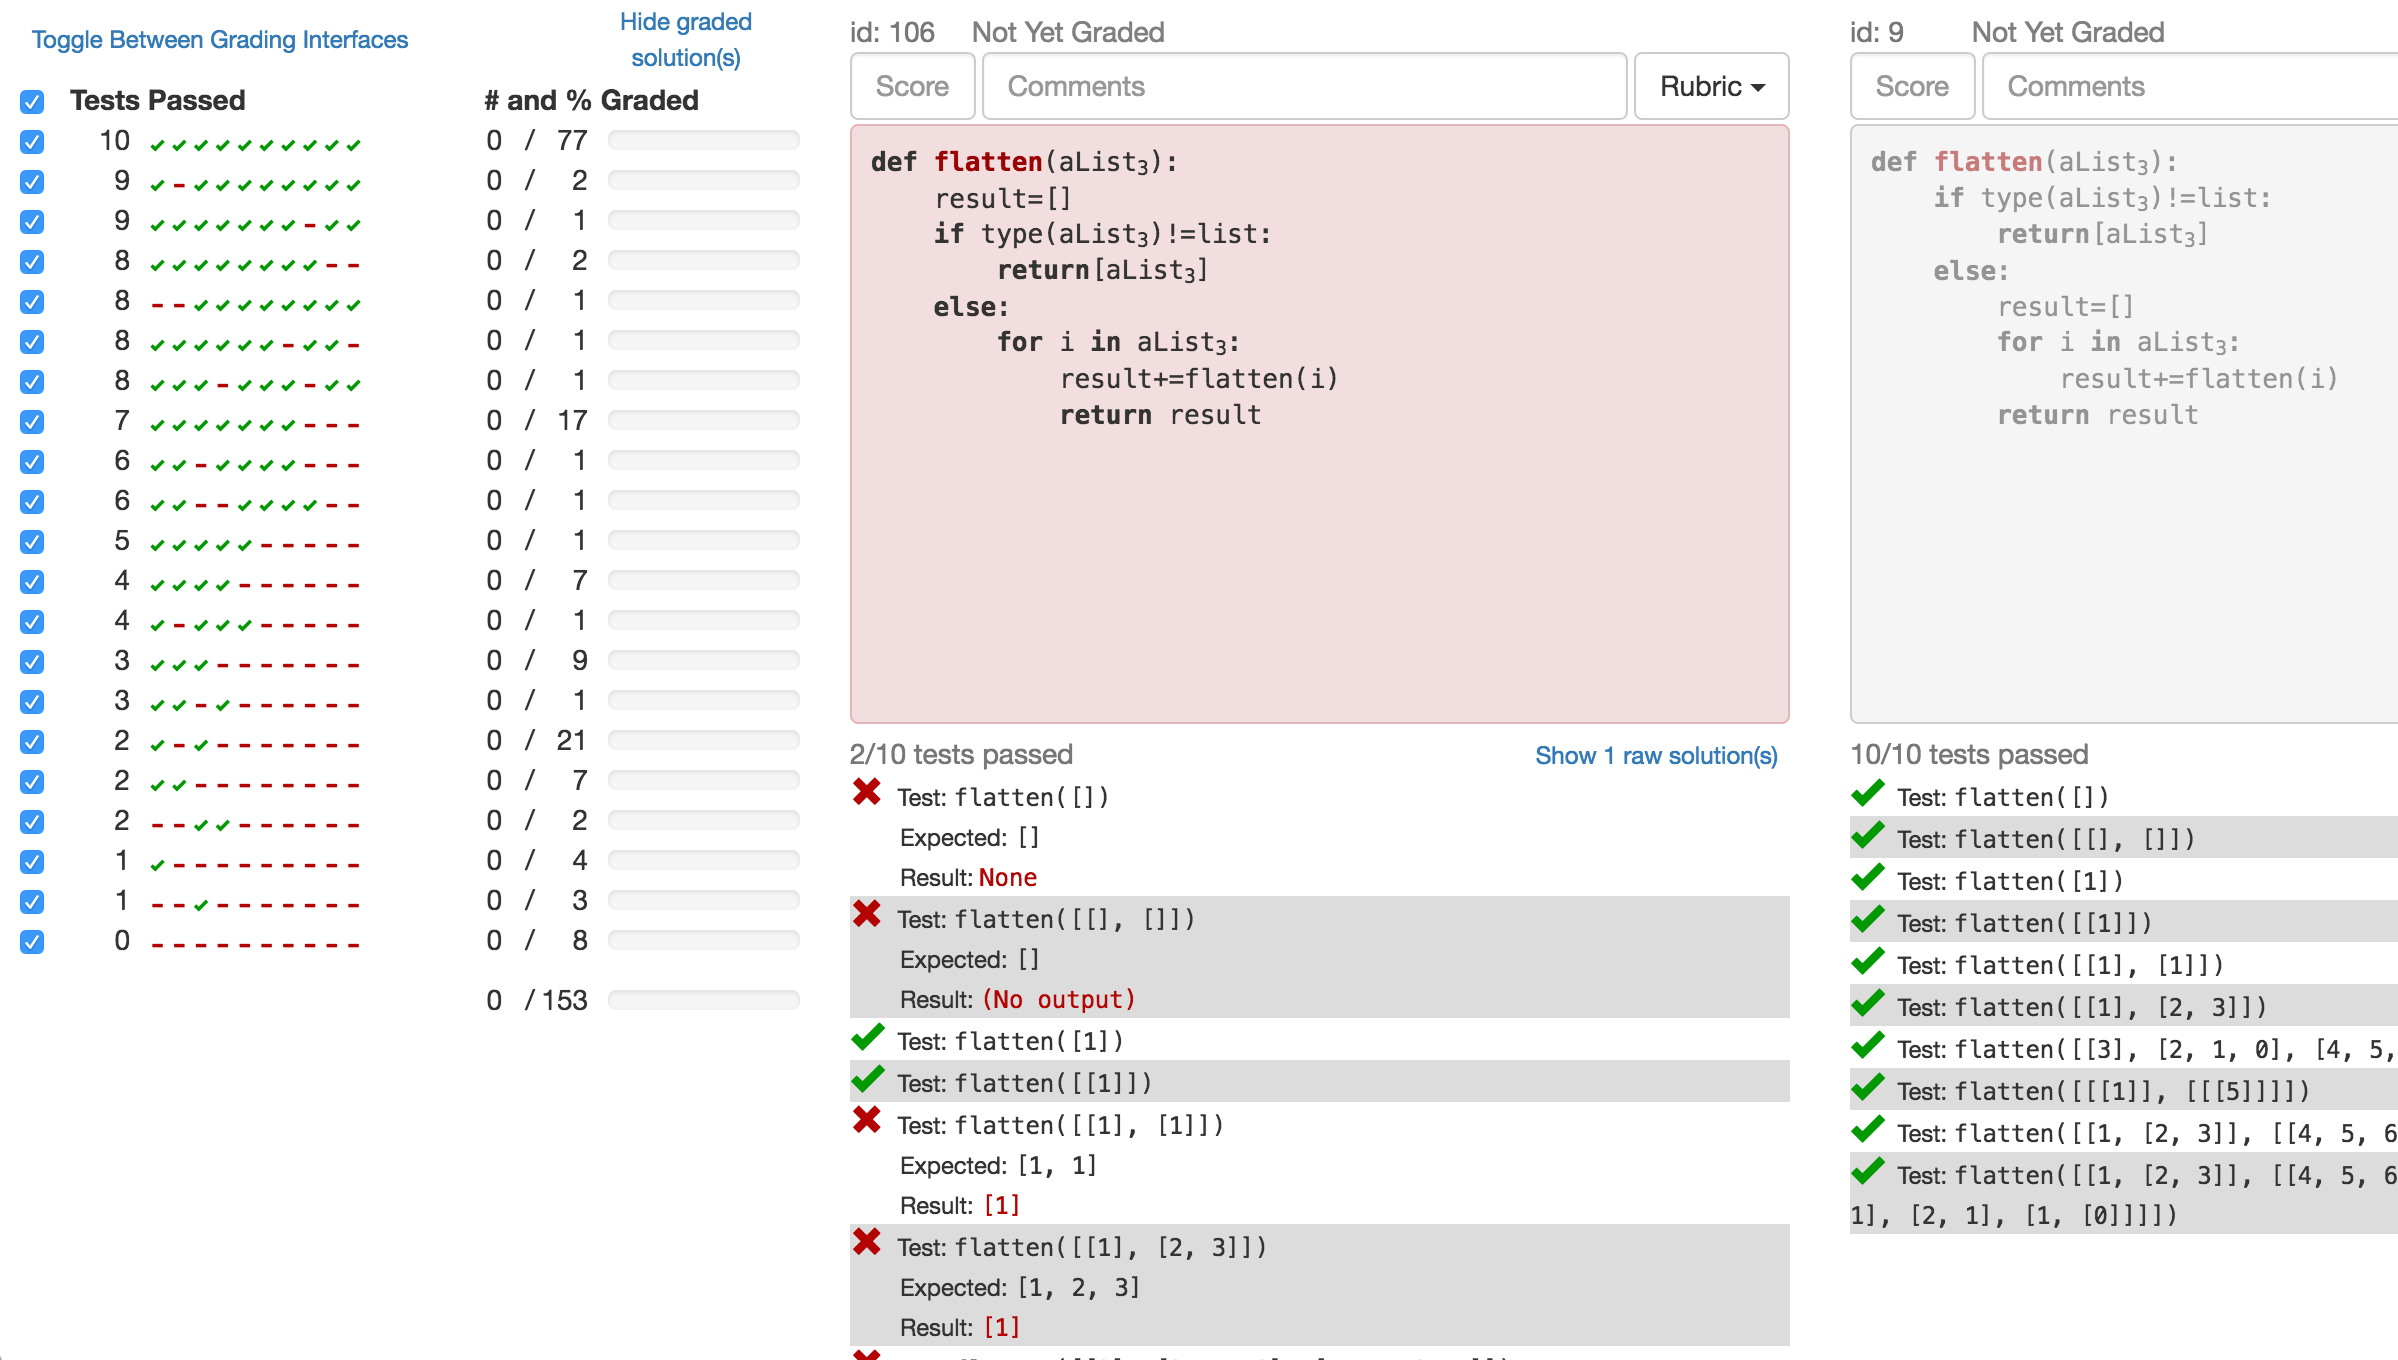
\includegraphics[width=\textwidth]{Body/figures/grovercode/figure_1}
\caption{The GroverCode user interface displaying solutions to an introductory Python programming exam problem, in which students are asked to implement a function to flatten a nested list of arbitrary depth.
}
\label{fig:whole_interface}
\end{figure} 

\begin{figure*}[t!]
    \centering
    \begin{subfigure}[b]{0.5\textwidth}
        \centering
        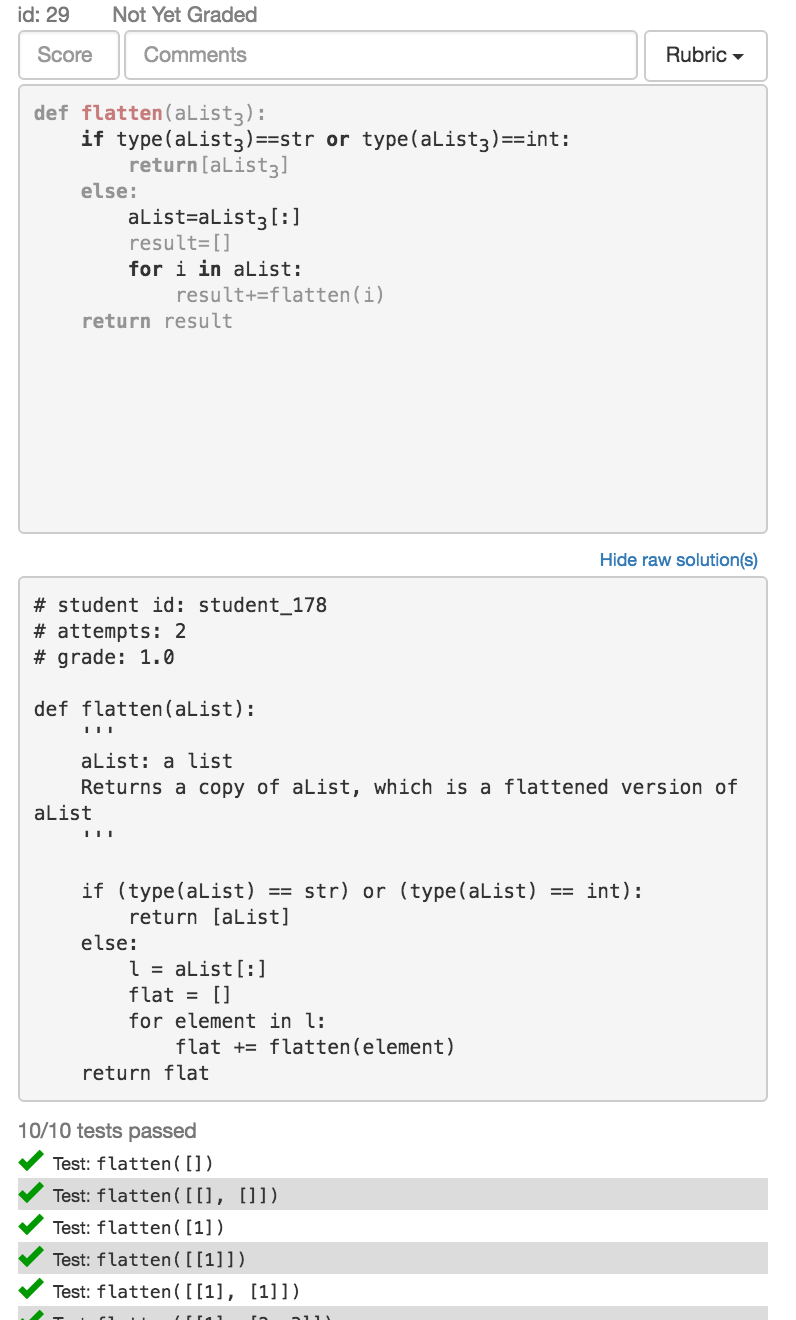
\includegraphics[height=4in]{Body/figures/grovercode/figure_2}
        \caption{A correct solution, its corresponding raw solution, and its performance on test cases, as displayed in GroverCode.}
        \label{fig:correct_stack}
    \end{subfigure}%
    ~ 
    \begin{subfigure}[b]{0.5\textwidth}
        \centering
        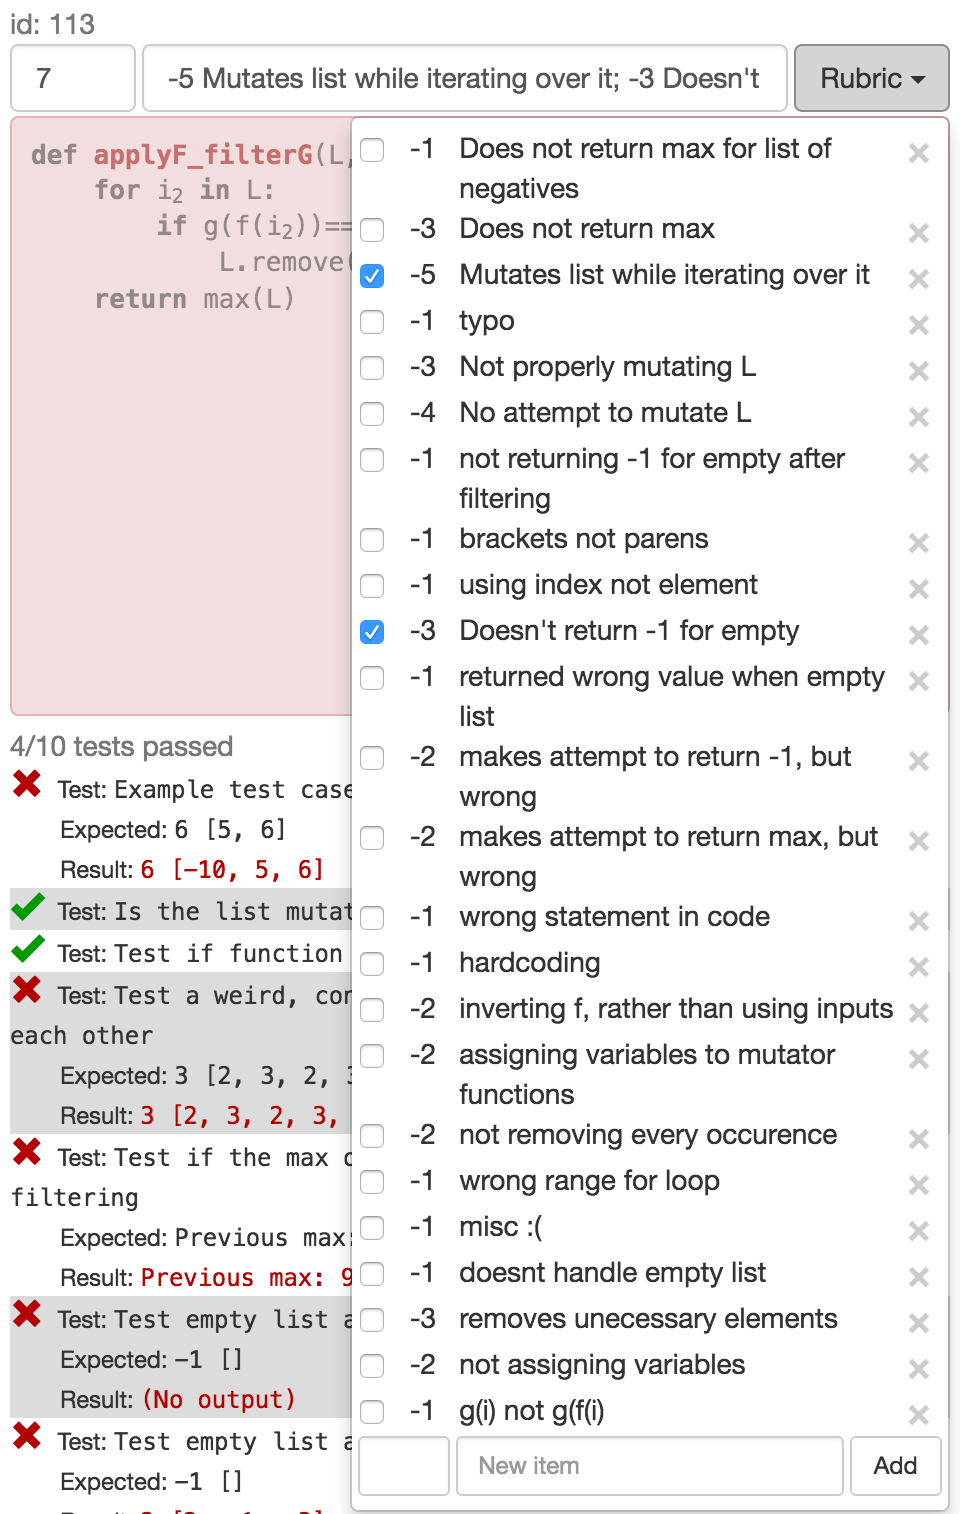
\includegraphics[height=4in]{Body/figures/grovercode/figure_3}
        \caption{An incorrect solution with the rubric dropdown menu open. Text for each of the checked items is automatically inserted in the comment box.}
        \label{fig:rubric}
    \end{subfigure}
    \caption{Correct and incorrect solutions, as rendered by GroverCode.}
\label{fig:correct_and_incorrect_stacks}
\end{figure*}

% \begin{figure}
% \centering
% 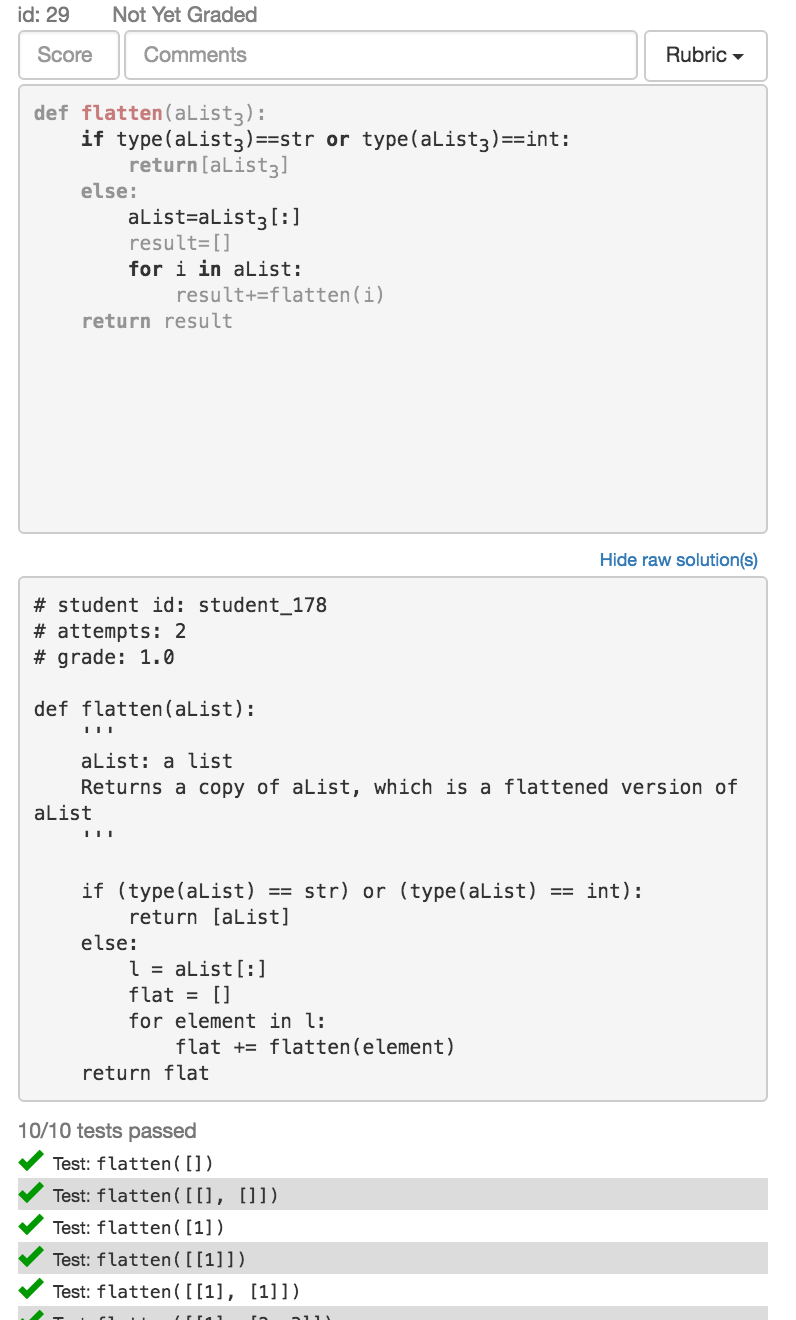
\includegraphics[width=0.5\textwidth]{Body/figures/grovercode/figure_2}
% \caption{A correct solution, its corresponding raw solution, and its performance on test cases, as displayed in GroverCode.}
% \label{fig:correct_stack}
% \end{figure}

% \begin{figure}
% \centering
% 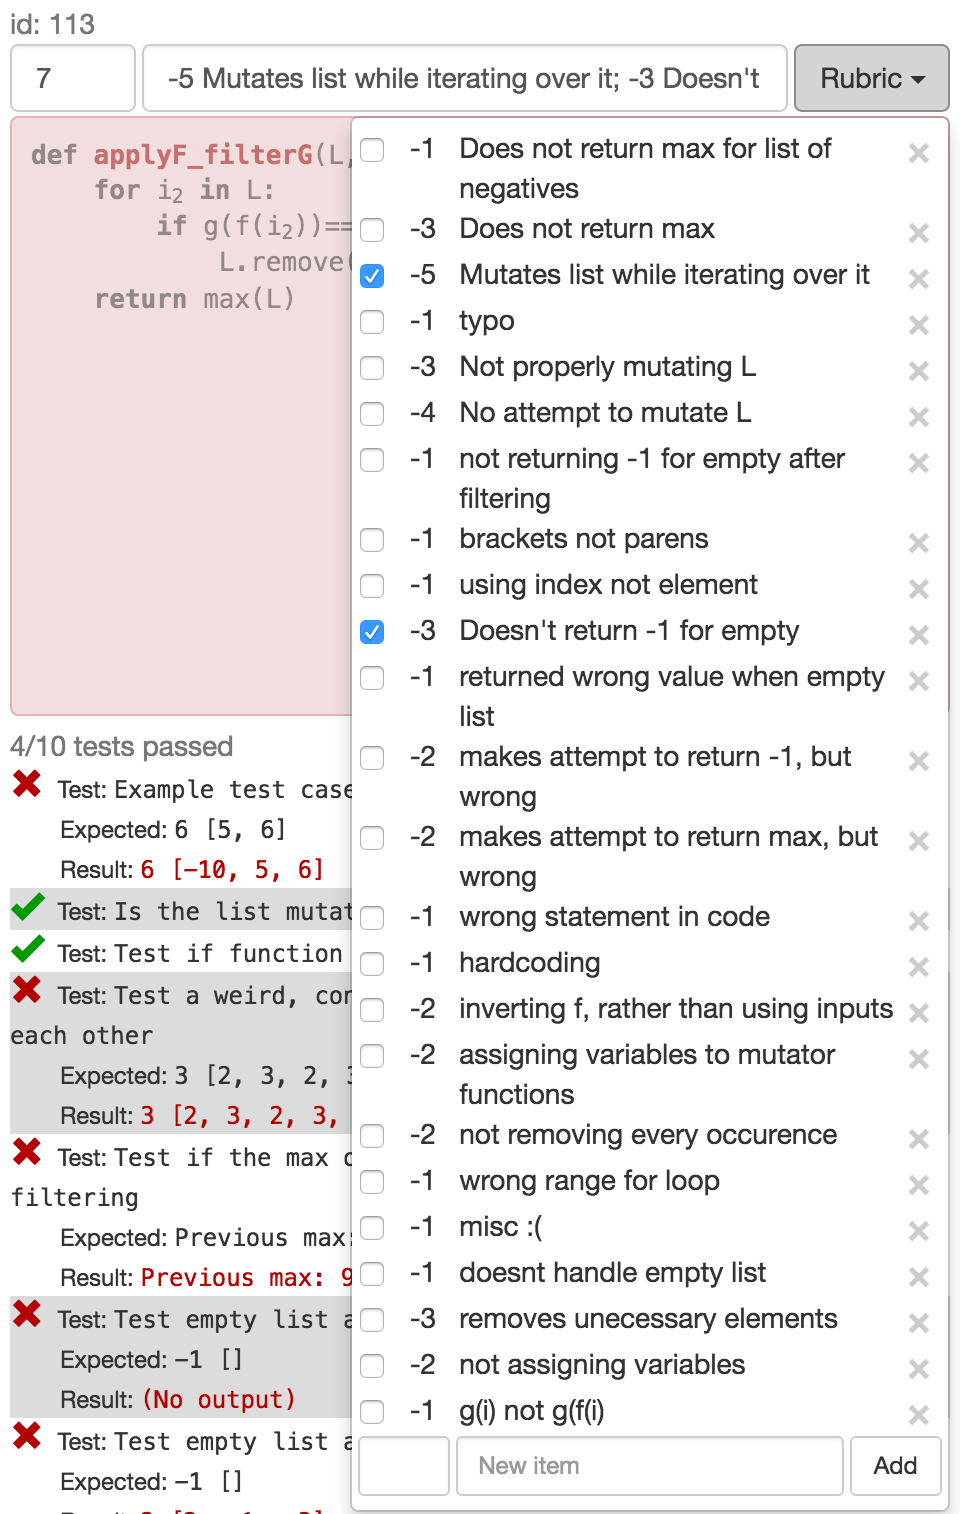
\includegraphics[width=0.5\textwidth]{Body/figures/grovercode/figure_3}
% \caption{A stack with the rubric dropdown menu open. Text for each of the checked items is automatically inserted in the comment box.}
% \label{fig:rubric}
% \end{figure}

The panel of progress indicators and filters, shown on the left side of Figure~\ref{fig:whole_interface}, helps teachers understand the distribution of solution behavior on test cases, track their grading progress, and grade sets of solutions that fail the same test cases one at a time. The rows of aligned sequences of green checks and red dashes represent error vectors, i.e., the pass/fail results with respect to the ordered list of teacher-specified test cases. The checkbox next to each error vector allows the teacher to selectively view subsets of solutions based on the particular tests they pass and fail. Solutions with the same error vectors may include similar mistakes. 

Like OverCode, GroverCode groups correct solutions into stacks. Grades are propagated to all the solutions in a stack. OverCode does not group incorrect solutions into stacks because the stacking process for incorrect solutions is too new and experimental for field deployment in an actual grading session. GroverCode still normalized all solutions, both correct and incorrect.

The grading performed by the 6.0001 staff was intellectually demanding. For example, many staff members attempted to correct incorrect solutions by hand to better undertstand how far off the student was from a correct answer. When raw solutions are shown in random order, one solution may have a different approach, behavior, and appearance from the next. The transition from grading one solution to the next can mean starting from scratch. In an attempt to minimize the cognitive load of switching from one solution to the next, the GroverCode user interface includes the following features:
\begin{itemize}
\item Horizontally aligned solutions for side-by-side comparison
\item Easy filtering of solutions by input-output behavior, i.e., their error vectors
\item Normalized variable names
\item Solutions ordered to minimize the distance between adjacent solutions with respect to a custom similarity metric defined in Stacey Terman's Master's of Engineering thesis~\cite{staceythesis}
\item Highlighted lines of code in each solution which differ from the previous solution in the horizontal list
\end{itemize}

In OverCode, a single-line difference between two solutions that affects variable behavior causes the variable renaming process to propagate naming differences to every line that mentions the affected variables. This non-locality of difference makes it harder to spot where the original syntactic difference between two platonic solutions is. As a result, the rendering of stacks in the GroverCode user interface is slightly different than in OverCode. Even if the normalized variable names are different between two syntactically identical lines of code in two different stacks, if the variables take on the same sequence of values {\it just within that line of code}, it will not be highlighted as different in the user interface. Only the line with the original syntactic difference will be highlighted.


\subsubsection{Implementation}~\label{subsec:grovercodepipeline}

The GroverCode implementation is a modification of the OverCode pipeline. Solutions which return an expected output for all test cases during the preprocessing step are categorized as correct, and all other solutions, having failed at least one test case, are categorized as incorrect. Correct solutions are normalized by the same process as was used in the original OverCode. 

In the original OverCode pipeline for correct solutions, variable behavior is assumed to hold enough semantic information to be the sole basis on which variable names are normalized. GroverCode applies this rule to incorrect solutions as well, but only for variables whose behavior matches a common variable in the correct solutions. This step may be error prone. Incorrect solutions are known to be wrong with respect to input-output behavior, the behavior of the variables within them is suspect too, even if it happens to match a common variable in a correct solution. %if a variable in an incorrect solution has the same behavior as a common variable in the correct solutions, GroverCode will rename the variable in the incorrect solution so it matches the common variable's name in the correct solutions.

%However, this renaming strategy may change in future versions of GroverCode because, 

In incorrect solutions, syntax, e.g., the operations applied to a variable, may be more helpful for normalizing variable names than behavior. For example, in an incorrect solution, a variable $i$ may be operated or depended on exactly the same way as a common variable in a correct solution. However, if an error somewhere else in the solution causes $i$ to behave differently, the original method of identifying common variables will be thrown off. %Based on this example, variables in incorrect solutions that are not already renamed based on behavior are renamed based on syntax.

The OverCode pipeline is modified for GroverCode to capture this syntactic information. The modified pipeline examines the program trace collected during preprocessing and the AST for each solution and compiles the following information for each line of code in each solution:
\begin{enumerate}
\item a template, i.e., the line of code with variables replaced by blanks, e.g., \texttt{\underline{\hspace{1em}} += 1} and \texttt{for \underline{\hspace{1em}} in range(\underline{\hspace{1em}}):}
\item an ordered list of the common variable behaviors and their normalized names corresponding to each blank in the line, e.g., the blank in \texttt{\underline{\hspace{1em}} += 1} can be associated with one of several common variables, depending on the rest of the solution
\item an ordered list of the sequences of values each blanked-out variable in the line took on during execution, e.g., the first blank in \texttt{for \underline{\hspace{1em}} in range(\underline{\hspace{1em}}):} might iterate through \texttt{1,2,3} while, with each visitation of this line during execution, the second blank stays constant at \texttt{[1,2,3],[1,2,3],[1,2,3]}
\end{enumerate}
Item 1 in this list, the template, captures the syntax of the line, ignoring the variables mentioned in it. Items 1 and 2 in this list together capture the information necessary to reconstruct the original normalized lines in OverCode. Items 1 and 3 capture the information necessary to tell what the variable behavior is just within that one line and whether two lines in two different stacks will be highlighted as different from each other. This information is also used for variable renaming in incorrect solutions.

\begin{table}
\centering
%Copied with permission from Terman~\cite{staceythesis}}\todo{get explicit permission}
\begin{tabular}{l l r}
%\hline
 &  & {\bf Location} \\
{\bf Example line of code} & {\bf Template} & {\bf of \texttt{exp}} \\
\hline
\footnotesize{\texttt{def power(base, exp):}} & \footnotesize{\texttt{def power(\underline{\hspace{1em}}},\underline{\hspace{1em}}):} & 1 \\
%\hline
\footnotesize{\texttt{while index <= exp:}} & \footnotesize{\texttt{while \underline{\hspace{1em}}<=\underline{\hspace{1em}}:}} & 1 \\
%\hline
\footnotesize{\texttt{return 1.0*base*power(base, exp-1)}} & \footnotesize{\texttt{return 1.0*\underline{\hspace{1em}}*\underline{\hspace{1em}}*power(\underline{\hspace{1em}},\underline{\hspace{1em}}-1)}} & 3 \\
%\hline
\footnotesize{\texttt{return base*power(base, exp-1)}} & \footnotesize{\texttt{return \underline{\hspace{1em}}*power(\underline{\hspace{1em}},\underline{\hspace{1em}}-1)}} & 2 \\
%\hline
\footnotesize{\texttt{return power(base, exp-1)*base}} & \footnotesize{\texttt{return power(\underline{\hspace{1em}},\underline{\hspace{1em}}-1)*\underline{\hspace{1em}}}} & 1 \\
%\hline
\footnotesize{\texttt{ans = base*power(base, exp-1)}} & \footnotesize{\texttt{\underline{\hspace{1em}}=\underline{\hspace{1em}}*power(\underline{\hspace{1em}},\underline{\hspace{1em}}-1)}} & 3 \\
%\hline
\footnotesize{\texttt{if exp <= 0:}} & \footnotesize{\texttt{if \underline{\hspace{1em}}<=0:}} & 0 \\
%\hline
\footnotesize{\texttt{if exp == 0:}} & \footnotesize{\texttt{if \underline{\hspace{1em}}==0:}} & 0 \\
%\hline
\footnotesize{\texttt{if exp >= 1:}} & \footnotesize{\texttt{if \underline{\hspace{1em}} >= 1:}} & 0 \\
%\hline
\footnotesize{\texttt{assert type(exp) is int and exp >= 0}} & \footnotesize{\texttt{assert type(\underline{\hspace{1em}}) is int and \underline{\hspace{1em}}>=0}} & 0, 1 \\
%\hline
\end{tabular}
\caption{\textbf{Example:} All templates and locations in which the abstract variable \texttt{exp}, the second argument to a recursive \texttt{power} function, appears. A location represents the index or indices of the blanks that the abstract variable occupies, where the first blank is index 0, the second is index 1, and so on. The second and third columns together form a template-location pair.} 
\label{tab:templatelocation}
\end{table}

The GroverCode normalization process uses this syntactic information, in addition to behavior, to identify and rename common variables. The template of a line, e.g., \texttt{for \underline{\hspace{1em}} in \underline{\hspace{1em}}:} is the syntax of the line with variable names removed. For each common variable in correct solutions, GroverCode counts how many times it appears in each template and in which location, represented as an index into the blanks in the template. Examples of templates and locations are shown in \autoref{tab:templatelocation}. If a yet-unrenamed variable in an incorrect solution appears in the exact same template-locations as a common variable in a correct solution, it will be renamed to match that common variable. If a variable in an incorrect solution is still not normalized, the counts of template-locations associated with each common variable in the correct solutions are used, as described in detail in Terman~\cite{staceythesis}, to infer the most likely common variable it could be renamed to, as long as a threshold for similarity is met. Otherwise, its original name is kept.





\subsubsection{Field Deployment}

Approximately two hundred students enrolled in 6.0001 during the spring 2016 semester, and nine instructors used GroverCode to grade nearly all student solutions. %Seven programming problems of a variety of difficulties were graded over the course of these two sessions.
The GroverCode analysis pipeline was run on both the midterm and final exam problems from the Spring 2016 semester of 6.0001, which had approximately 200 students enrolled. These exams contained seven programming problems in total, and between 133 and 189 solutions per problem made it through the analysis pipeline to be displayed in the user interface. The midterm problem prompts were:
\begin{itemize}
\item \texttt{power} (q4): Write a recursive function to calculate the exponential \texttt{base} to the power \texttt{exp}.
\item \texttt{give\_and\_take} (q5): Given a dictionary \texttt{d} and a list \texttt{L}, return a new dictionary that contains the keys of \texttt{d}. Map each key to its value in \texttt{d} plus one if the key is contained in \texttt{L}, and its value in d minus one if the key is not contained in \texttt{L}.
\item \texttt{closest\_power} (q6): Given an integer base and a target integer \texttt{num}, find the integer exponent that minimizes the difference between \texttt{num} and \texttt{base} to the power of exponent, choosing the smaller exponent in the case of a tie.
\end{itemize}
The final problem prompts were:
\begin{itemize}
\item \texttt{deep\_reverse} (q4): Write a function that takes a list of lists of integers \texttt{L}, and reverses \texttt{L} and each element of \texttt{L} in place.
\item \texttt{applyF\_filterG} (q5): Write a function that takes three arguments: a list of integers \texttt{L}, a function \texttt{f} that takes an integer and returns an integer, and a function \texttt{g} that takes an integer and returns a boolean. Remove elements from \texttt{L} such that for each remaining element \texttt{i}, \texttt{f(g(i))} returns \texttt{True}. Return the largest element of the mutated list, or -1 if the list is empty after mutation.
\item \texttt{MITCampus} (q6): Given the definitions of two classes: \texttt{Location}, which represents a two-dimensional coordinate point, and \texttt{Campus}, which represents a college campus centered at a particular \texttt{Location}, fill in several methods in the \texttt{MITCampus} class, a subclass of \texttt{Campus} that represents a college campus with tents at various \texttt{Locations}.
\item \texttt{longest\_run} (q7): Write a function that takes a list of integers \texttt{L}, finds the longest run of either monotonically increasing or monotonically decreasing integers in \texttt{L}, and returns the sum of this run.
\end{itemize}
For each problem processed during the field deployments, an example of a staff-written correct solution is included in the Appendix.

Using the GroverCode user interface, nine instructors, including one lecturer and eight teaching assistants (TAs) graded these solutions as part of their official grading responsibilities. Stacey Terman, the Master's of Engineering student who implemented most of GroverCode, was one of these TAs. GroverCode logged TA grading events, such as adding or applying rubric items and point values to solutions. TAs hand-graded solutions that did not successfully pass through the GroverCode pipeline. The observer (the author of this thesis) took extensive notes during each day-long grading session to capture spontaneous feature requests as well as bugs and complaints. 

%\begin{comment}
% {\bf Programming Exam Problems}

%Given the increasing difficulty of these exam problems, the following numbers dropped between the midterm and the final: the number of students present to take the exam, the number of students who submitted any solution to a given problem before the test period ended, and the number of correct solutions that could be clustered.

\subsubsection{Pipeline Evaluation}

Table~\ref{table:num_submissions} shows the number of solutions submitted for each problem and the number successfully processed by the GroverCode pipeline. Table~\ref{table:cluster_stats} captures the scale of the variation as well as some clustering statistics. Table~\ref{table:renametype} summarizes the counts of the various mechanims by which variables in incorrect solutions were normalized.

\begin{table}[h!]
\centering
\begin{tabular}{l r|r|r|r|r|r|r}
%\hline
& \multicolumn{3}{c}{Quiz} & \multicolumn{4}{c}{Final} \\
%\cline{2-8}
& q4 & q5 & q6 & q4 & q5 & q6 & q7 \\
\hline
Submissions & 193 & 193 & 193 & 175 & 173 & 170 & 165 \\
\hline
Mean lines per solution & 9.9 & 16.9 & 19.8 & 12.3 & 20.9 & 50.0 & 41.8 \\
\hline
Solutions & 186 & 189 & 168  & 170 & 166  & 134 & 133 \\
successfully processed & 96\% & 98\% & 87\% & 97\% & 96\% & 79\% & 81\% \\
%\hline
\end{tabular}
\caption{Number of solutions submitted and successfully processed by GroverCode for each problem in the dataset. Reasons why a solution might not make it through the pipeline include syntax errors and memory management issues caused by students making inappropriate function calls.}
\label{table:num_submissions}
\end{table}

\begin{table}[!ht]
\centering
\begin{tabular}{l r|r|r|r|r|r|r}
%\hline
& \multicolumn{3}{c}{Quiz} & \multicolumn{4}{c}{Final} \\
%\cline{2-8}
& q4 & q5 & q6 & q4 & q5 & q6 & q7 \\
\hline
Correct solutions & 182 & 160 & 94 & 96 & 49 & 16 & 12 \\
 & 94\% & 82\% & 49\% & 55\% & 28\% & 9\% & 7\% \\
\hline
Incorrect solutions & 4 & 29 & 74 & 74 & 117 & 118 & 121 \\
\hline
Test cases & 10 & 15 & 25 & 11 & 10 & 17 & 28 \\
\hline
Distinct error signatures & 6 & 16 & 36 & 12 & 38 & 57 & 42 \\
\hline
Correct stacks & 40 & 84 & 93 & 47 & 46 & 16 & 12 \\
\hline
Stacks with > 1 solution & 13 & 18 & 1 & 8 & 2 & 0 & 0 \\
\hline
Solutions in stacks & 151 & 94 & 2 & 57 & 5 & 0 & 0 \\
%\hline
\end{tabular}
\caption{The degree of variation in input-output behavior and statistics about stack sizes.}
\label{table:cluster_stats}
\end{table}

\begin{table}
\centering
\begin{tabular}{l c|c|c|c|c|c|c}
%\hline
& \multicolumn{3}{c}{Quiz} & \multicolumn{4}{c}{Final} \\
%\cline{2-8}
& q4 & q5 & q6 & q4 & q5 & q6 & q7 \\
\hline
Variables in incorrect submissions & 15 & 149 & 482 & 289 & 550 & 559 & 859 \\
\hline
Variables renamed based on values & 14 & 84 & 266 & 97 & 246 & 97 & 187 \\
\hline
Variables renamed based on templates & 0 & 58 & 166 & 136 & 264 & 188 & 489 \\
\hline
Variables not renamed & 1 & 7 & 50 & 56 & 40 & 274 & 183 \\
%\hline
\end{tabular}
\caption{Statistics about variables renaming based on different heuristics in the GroverCode normalization process.}
\label{table:renametype}
\end{table}
%\end{comment}
 
\subsubsection{Discussion}

GroverCode was particularly appreciated on simpler problems where GroverCode clustered correct solutions together to be graded by a single action. Under these conditions, the clustering capability GroverCode inherits from OverCode amplified teacher effort.

Variable renaming was, for simpler programming problems, an invisible and possibly slightly confusing helping hand. One grader remarked, out loud: ``Why is everyone naming their iterator variable `i'?'' at which point he had to be reminded of the variable renaming process. 

When applied to more complex solutions, the normalization process was at times more harmful than helpful for teacher comprehension. As solutions became more varied and structurally complex, graders started toggling off normalization because the renaming of variables, removal of comments, and formatting standardization was removing clues they needed in order to understand student intent.

The feature for grouping solutions based on their behavior on test cases was appreciated regardless of solution complexity. While it was difficult to get direct feedback on the helpfulness of pair-wise difference highlighting and optimized solution ordering, graders heavily used and appreciated the ability to filter and grade solutions one error vector at a time. At least one grader remarked aloud that it seemed like many of the solution with the same error vector made similar mistakes. Therefore filtering by error vector may have been one of the stronger contributors to any hypothetical decreased cognitive load due to using GroverCode over the status quo of random assignment to solutions in a CSV file.

%\todo{DNHT: add to related work Appropriately chosen latent variable models have already been used in the past to model open-source code and answers to open-response mathematical questions.}

\section{Conclusion}
OverCode is a novel system for visualizing thousands of Python programming solutions that helps teachers explore the variations among them. Unlike previous approaches, OverCode uses a lightweight static and dynamic analysis to generate platonic solutions that represent stacks of similar solutions in an interactive user interface. It allows teachers to filter stacks by normalized lines of code and to further merge different stacks by composing rewrite rules. As observed in two user studies with a total of 24 current and potential teaching assistants, OverCode allowed teachers to more quickly develop a high-level view of students' understanding and misconceptions, and provide feedback that is relevant to more student solutions. 

GroverCode, an extension of OverCode which handles incorrect solutions, is a new tool for triaging and hand-grading solutions. It was successfully deployed in the field as the tool for grading the midterm and final exams of MIT's 6.0001 course, ``Introduction to Computer Science and Programming in Python''. Based on teachers' appreciation of the interface over the existing alternatives, GroverCode will continue to be deployed in the field to ease the subjective psychological burden of grading hundreds of Python programs. %I believe an information visualization approach is necessary for teachers to explore the variations among solutions at the scale of MOOCs, and OverCode is an important step towards that goal.
%\todo{make sure evidence of teacher's appreciate is included}
%\chapter{Foobaz: Feedback on Variable Names at Scale}\label{chapter:foobaz}

%Current traditional feedback methods, such as hand-grading student code for substance and style, are labor intensive and do not scale. We created a user interface that addresses feedback at scale for a particular and important aspect of code quality: variable names. We built this user interface on top of an existing back-end that distinguishes variables by their behavior in the program. Therefore our interface not only allows teachers to comment on poor variable names, they can comment on names that mislead the reader about the variable's role in the program. We ran two user studies in which 10 teachers and 6 students created and received feedback, respectively. The interface helped teachers give personalized variable name feedback on thousands of student solutions from an edX introductory programming MOOC. In the second study, students composed solutions to the same programming assignments and immediately received personalized quizzes composed by teachers in the previous user study. 

%\section{Introduction}

Current traditional feedback methods for solutions to programming assignments include hand-grading student code for substance and style. Unfortunately, those methods are labor intensive, potentially inconsistent across graders, and do not scale to the sizes associated with Massive Open Online Courses (MOOCs). The scaling difficulty is particularly important when considering that  some residential course enrollments at prominent universities, like UC Berkeley's CS61A, are rising above the thousand-student mark \cite{biggestClass}. Some Computer Science teachers, such as MIT's John Guttag and Ana Bell, are simultaneously teaching hundreds of students in residential programming courses and thousands of online students in MOOC versions.

Variable naming is a specific, important aspect of writing readable, maintainable code, and many teachers want to give feedback on it. The quality of a name is most easily judged when its role within the surrounding code is known. However, at scale, teachers cannot read every solution. Programming education at scale opens up new challenges for processing and presenting thousands of solutions so that teachers can more easily view them. Teachers also cannot write comments on each solution. This difficulty motivates the creation of tools that help teachers give customized feedback to subsets of students for whom that feedback is relevant.

This chapter introduce Foobaz, a user interface for giving tailored feedback on student variable names at scale. Foobaz enables teachers to explore and comment on the quality of student-chosen variable names, given the role the variables play in students' code (see Figure \ref{fig:figure2}). A variable's role is a function of the sequence of values that the variable contains during program execution. The variety of student-chosen variable names for each role makes evaluating every one prohibitive. Using Foobaz, the teacher can label a small subset of good and bad names for each role. 

Foobaz then uses these labeled variable names to create pedagogically valuable active learning exercises in the format of multiple choice quizzes. These quizzes are a form of feedback for many more students than just those whose variable names receive a teacher's label. The quizzes also allow students to see examples of good and bad alternatives, rather than just receive a label on one of their own names. 

Foobaz personalizes teacher quizzes for each student, so that students can consider good and bad names for variables that exist in their own solutions. Personalized quizzes render the student's original code submission with a specific variable replaced by an arbitrary symbol. The quiz presents the student with several variable names as candidate replacements for the symbol, one of which may be the student's original choice. The student selects appropriate labels for the variable names before checking their labels against teacher labels and comments.

In two user studies, the capabilities and workflow enabled by this novel interface are demonstrated. The first study shows that the interface helped teachers give personalized variable name feedback on thousands of student solutions from an introductory programming MOOC on edX. In the second study, students composed solutions to the same programming exercises and received personalized quizzes generated with Foobaz by teachers in the first study.

\todo{remove we from the rest of this chapter}

\section{User Interface}

Consider an introductory programming MOOC where thousands of students submit correct solutions to a programming exercise. Imagine that many of these solutions include a variable that takes on the same sequence of values, like a running sum of the elements in an input argument. While most students decide to name this variable $result$, others decide to give it obscure or less descriptive names like $p$, $val1$.

The quality of a variable's name is most easily judged when the teacher understands its algorithmic role and relationship to other variable names within the surrounding code. At scale, this can be difficult and frustrating, because while variable roles can be repetitive across many solutions (e.g., a particular running sum), their names can be unpredictable ($result$, $val1$, $s$). Instead of browsing student submissions in a linear fashion, it would be better if the teacher could provide feedback on the basis of variable roles.

In Foobaz, teachers can browse \emph{stacks} of student submissions. A stack is a set of solutions whose code is identical after normalizing formatting and variable names, removing comments, and ignoring the exact order of statements. Within a stack, the teacher can browse the different sets of variable names that students chose, label some of them as, e.g., ``too short'' or ``misleading,'' and add comments. 

Teacher labels and comments are used to provide students with tailored feedback in the form of personalized quizzes on variable names. By providing feedback on only a few variable names, personalized quizzes are generated that are potentially relevant to thousands of students. Foobaz is distinct from powergrading systems: instead of grading as many names as possible, the system produces personalized quizzes that have excellent examples of good and bad variable names students would not otherwise get to see and learn from.

\subsection{Producing Stacks and Common Variables}
Foobaz enables feedback at scale because teachers can browse solutions on the basis of \emph{stacks of similar solutions} and \emph{common variables}. These groupings are automatically produced by the OverCode analysis pipeline, which starts by executing each student's solution on a single test case and tracking the sequences of values that variables take on. Common variables are identified as those that behave the same way (i.e., take on the same sequence of values) across multiple solutions. Raw solutions are then normalized by renaming instances of common variables with their most popular names, as well as removing comments and extra whitespace. Normalized solutions that have the same set of lines can be grouped together into a \emph{stack}, with a single representative on top for the teacher to read. 

The stacking performed by the system directly reduces the number of implementations that a teacher needs to analyze in order to provide feedback to the majority of the class. Furthermore, Foobaz is sensitive to \emph{variable roles}, meaning that variables that behave the same across different stacks are linked together as a single common variable. The result is that feedback provided for a variable in one stack is propagated to variables that play out the same behavior in \emph{other} stacks.

\subsection{Rating Variable Names}

The Foobaz interface lets the teacher rate variable names in the context of their role in the program. Figure \ref{fig:figure2} shows the teacher's view while they perform this task. 

The teacher is presented with a scrollable list of stacks. Each stack is represented as normalized stack code followed by a table of alternative variable names. Since some of the tables are taller than the screen, the normalized stack code is pinned to the screen in such a way that it remains visible until the next stack is scrolled into view.

Each column of the table represents the common variables occurring in the stack, where each common variable's most popular name serves as the column header. Each row of the table represents a unique set of variable names used in a solution (e.g., $secretWord$, $lettersGuessed$, $guessedWord$, $char$). We show \emph{sets} of variable name choices, rather than independent columns of variable names, because we found in early pilot testing that variable names can at times make more sense when seen as a group, rather than as individual naming decisions. This helps give teachers the context and confidence to assign quality judgments.

As the teacher brushes over the names of a common variable in the table, its occurrences in the normalized code are highlighted, so they can develop an understanding of the variable's role in the solution. The teacher can then go down the list of student-chosen names, rating as many of them as they desire using three different labels: ``misleading or vague,'' ``too short,'' or ``fine.'' These labels were based on early pilot testing with beginner programmers but future iterations of Foobaz may support teacher-added labels. Next to each name, they can also see how frequently it was given to that common variable across all solutions in the dataset, and can sort the entire table by this frequency. In order to draw teachers' attention to student-chosen variable names, variables with names that match one of given parameter names provided with the homework prompt are greyed out. The long tail of infrequently used names can be a place where both the best and worst examples of names can be found.

It is important to note that each common variable is likely to occur in multiple stacks. When the teacher selects a particular name, or set of names, for a common variable, occurrences in other stacks are highlighted as well. When they assign a label to a name, the label is propagated to all uses of the name for that common variable, across all the stacks. This has the effect of ``filling down'' the teacher's annotations. As teachers scroll down, they see that much of their feedback has been propagated for them, letting them focus on the remaining best and worst examples they might find. 

A progress bar at the top of the page indicates the coverage of their feedback across all variable names. Since teachers were motivated by the progress bar to maximize their coverage, we provided a button which would select and scroll into view the next most popular, yet unlabeled name for a common variable. Also included to maximize efficiency, the interface supports navigation through the variable names in the table using arrow keys. Teachers can also press hotkeys to rate variables instead of clicking on one of the three quality judgments, e.g., press $2$ to rate a variable name as ``too short.''

\begin{figure}
\centering
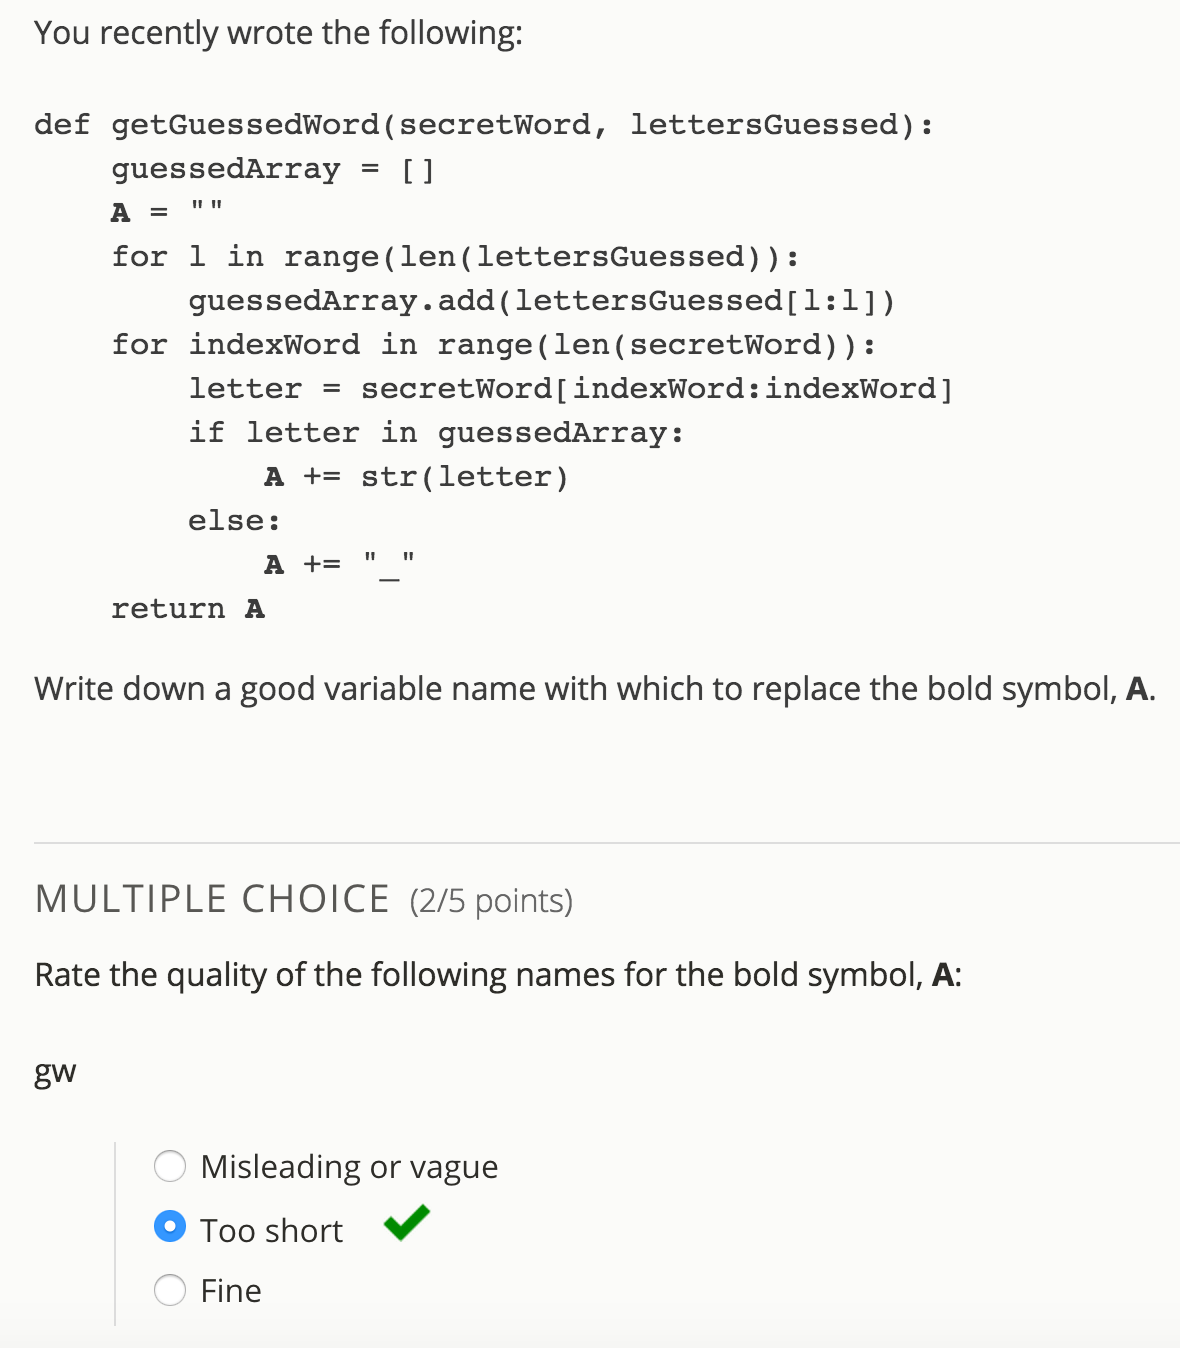
\includegraphics[width=0.95\columnwidth]{Body/figures/foobaz/feedbackQuizExample.png}
\caption{A personalized quiz as seen by the student, delivered by edX infrastructure. Students are shown their own code, with a variable name replaced by an arbitrary symbol, followed by variable names for the student to consider and label using the same labels that were available to the teacher. After the student has submitted their own judgments, the teacher's labels are revealed, along with their explanatory comments.}~\label{fig:figure4}
\end{figure}

\begin{figure}
\begin{minipage}{1\columnwidth}
\centering
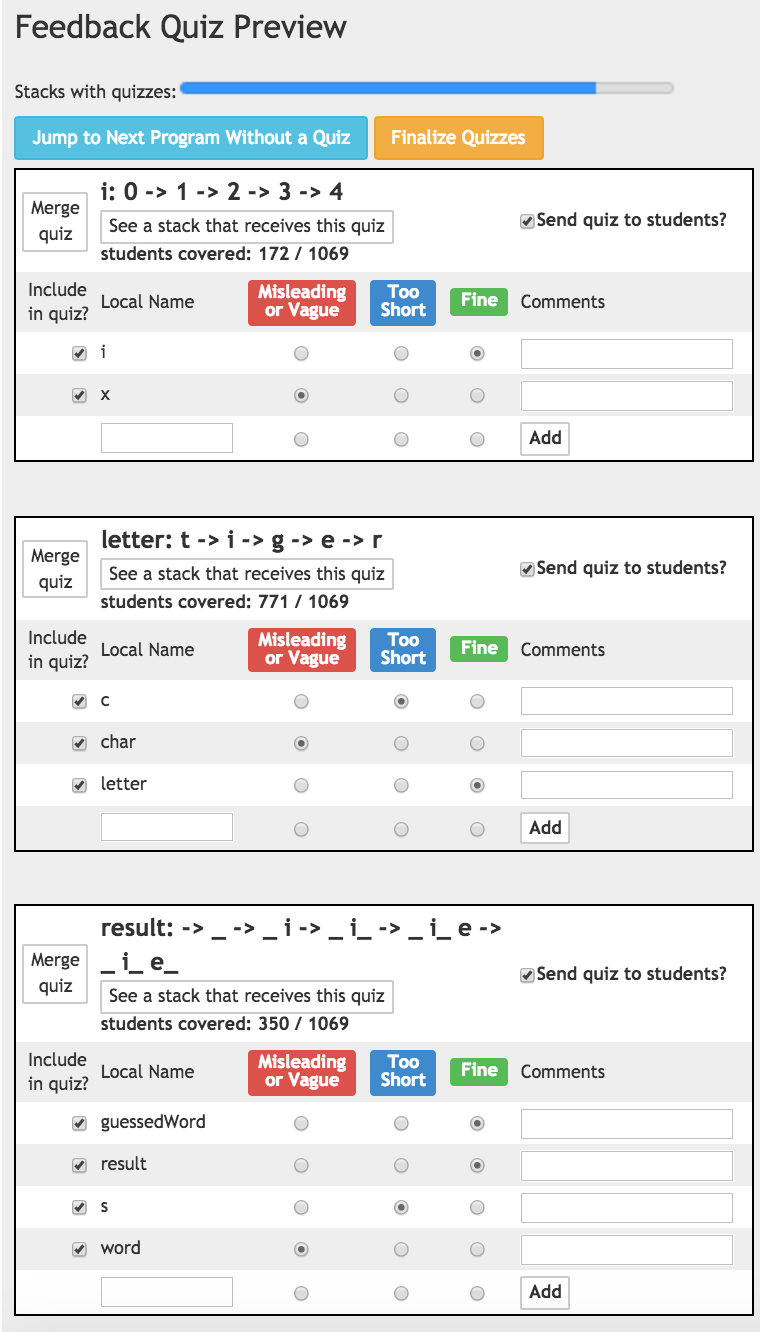
\includegraphics[width=0.85\columnwidth]{Body/figures/foobaz/quizPreviewHangman.png}
\caption{The quiz preview pane of the Foobaz teacher interface. Variable behavior was logged by running all solutions on a common test case. This particular teacher created quizzes for the common variable $i$ that iterates through indices of a list, the common variable $letter$, which iterates through the characters in an input string, and the common variable $result$, which accumulates one of the acceptable return values, `$\_i\_e\_$.'}~\label{fig:figure3}
\end{minipage}

\bigskip
\begin{minipage}{1\columnwidth}
\centering
\begin{tabular} {|l|l|r|}
\hline
\tabhead{Problem Description} & \tabhead{Source} & \tabhead{Solutions} \\ \hline \hline
\codevar{iterPower} & 6.00x (edX) & 3875 \\ \hline
\codevar{hangman} & 6.00x (edX) & 1118 \\ \hline
\codevar{computeDerivative} & 6.00x (edX) & 1433 \\ \hline
\codevar{dotProduct} & 6.0001 (residential) & 229 \\ \hline
\end{tabular}
\caption{Number of solutions in datasets.}
\label{solutioncounttable}
\end{minipage}

\bigskip
\begin{minipage}{1\columnwidth}
\centering
\begin{tabular}{|l|r|r|r|r|}
\hline
\tabhead{Problem} & \tabhead{Misleading} & \tabhead{Too short} & \tabhead{Good} & \tabhead{Total names} \\
& \tabhead{or Vague} & & & \\ \hline \hline
\codevar{iterPower} & 3 & 3 & 15 & 929 \\ \hline
\codevar{hangman} &7 & 4 & 10 & 763 \\ \hline
\codevar{compDeriv} & 6 & 5 & 10 & 670 \\ \hline
\codevar{dotProduct} & 11 & 3 & 17 & 180 \\ \hline
\end{tabular}
\caption{Subjects in Study 1, on average, labeled a small fraction of the total names, covering all three provided name categories.}~\label{tab:averageLabeling}
\end{minipage}

\end{figure}

\subsection{Making Quizzes}

Each quiz is an active learning exercise that asks the student to think about good and bad names for a common variable. Quizzes begin by showing a solution with that common variable's name replaced by an arbitrary symbol everywhere it occurs. In a personalized quiz, the solution is the student's own, as shown in Figure \ref{fig:figure4}. The quiz presents the student with several variable names as candidate replacements for the symbol, one of which may be the student's original choice. The student labels these names before checking their labels against the teacher's. If a student's solution includes a particular common variable, then that student can receive a personalized version of the quiz about that variable.

As teachers rate variables by attaching labels to them, quizzes are created with these names as their good and bad examples. Using the Toggle Quiz Preview button, teachers can see a preview of the quizzes (Figure \ref{fig:figure3}) alongside the scrollable list of stacks and watch the quizzes grow as they rate more names. They can hide the quiz preview to reduce visual clutter while they explore all the stacks, common variables, and interesting alternative names.

If two different common variables perform the same conceptual role in student solutions but do not go through the exact same sequence of values, then the teacher can use the ``Merge'' button to combine the quizzes about each common variable into a single quiz. This quiz becomes relevant to students who have either common variable in their own solution and can be sent out to both groups.

Ultimately, the teachers' goal is to provide pedagogically valuable personalized quizzes to as many of the hundreds or thousands of students in the course as possible. Analogous to the progress bar for variable names, the quiz preview pane includes a progress bar for the number of stacks of solutions that will receive at least one quiz. Like the previously discussed button for selecting the next most popular unlabeled name, the quiz preview pane also includes a button for jumping to the next largest stack of student solutions that do not yet have any quizzes. If the teacher deems one of their automatically populated quizzes to be not pedagogically valuable, then they can uncheck the option to send that quiz back to students. To provide more illustrative examples that might not have been produced in student solutions, teachers can add their own custom good and bad variable name examples and write explanations in the comment field associated with each alternative name.

\section{Evaluation}

We evaluate Foobaz's teacher and student-facing interfaces with two consecutive user studies, one for each population. In order to evaluate Foobaz's scalability, the solutions seen by teachers were collected from MOOCs with thousands of students and a residential college class of several hundred students.

\subsection{Datasets}

We evaluated Foobaz on sets of correct solutions to four different programming exercises, ranging in size from a couple hundred to several thousand solutions, collected from 6.00x, an introductory programming course in Python that was offered on edX in the fall of 2012, and 6.0001, a residential introductory programming course in Python offered at MIT in the fall of 2014 (see Figure \ref{solutioncounttable}). The four exercises, referred to here as \codevar{iterPower}, \codevar{hangman}, \codevar{dotProduct}, and \codevar{computeDerivative}, are representative of typical exercises that students solve in the early weeks of an introductory programming course. They have varying levels of complexity and ask students to perform loop computation over three fundamental Python data types, integers, strings, and lists.

\subsection{Teacher Study}

During the initial briefing, teachers were informed that they would be looking at solutions that had already passed an autograder and instructed to focus only on variable names, ignoring other aspects of code style, structure, and correctness. Teachers were invited to look over a page in a browser with all solutions concatenated in a random order into a flat list of boxed, syntax-highlighted code. We chose this design as our baseline to emulate existing methods of reviewing student functions. 

Using this baseline interface, teachers were asked first to rate as many good and bad variable names as possible, with an eye toward maximizing coverage of names (Task Part 1). Next, the teachers were shown an example of a quiz and were asked to compose their own by listing variable names and labeling them as good or bad with whatever short descriptors and explanatory comments they wished (Task Part 2). Participants were given 5 minutes for each task, and then asked to fill out a survey about their experience. (The answers to two of these surveys were lost so we only report survey results from 8 of the 10 participants.)

Participants learned about the Foobaz interface by watching a tutorial video. This training process took between 10 and 15 minutes depending on the dataset shown in the video. Participants were encouraged to hold their questions to the end, and answer them by interacting with the interface. 

Participants performed both Task Part 1 and 2 on a third dataset of solutions in the Foobaz teacher interface. Participants were asked to spend 5 minutes to perform each task, though some decided to spend more time. They filled out the same surveys about their experience again, followed by a final survey about which features of the Foobaz interface they found helpful. 

\subsubsection{Apparatus}

In all sessions, we used a laptop with a 15.4-inch 2880x1800 pixel Retina screen. All participants' interactions with the system were logged with timestamps using Meteor collections.

\subsubsection{Participants}

We recruited 10 participants (6 female) with ages between 20 and 29 ($\mu=23.1$, $\sigma=2.7$) through computer science-specific and campus-specific mailing lists and Facebook groups. All participants self-reported that they had been a grader, lab assistant, or teaching assistant for a Python course. 

\subsubsection{Results}

\textbf{Problems with Baseline}. When asked to comment on good and bad variable names based on the baseline interface, most teachers immediately began scrolling through solutions one by one, taking notes as they went, fully aware that they would only be able to skim a small, random fraction of the total number of solutions. The sheer volume of solutions was overwhelming to some. 

Results of the post-baseline survey reinforce critical usability issues with the status quo that Foobaz was designed to address. In these survey responses, teachers expressed an appreciation for the simplicity, readability, and searchability of the baseline interface but wished that the endless stream of often very similar solutions could be summarized or ``de-duped'' before they had to read through them. One teacher requested that variables be automatically identified, so that all references to a variable can be highlighted. This may have been a direct consequence of the fact that it was not possible to search for all the occurrences of the variable name $i$ without the browser also highlighting all the $i$'s within the rest of the names and keywords, e.g., the $i$ in ``if.'' Another teacher requested an automated count of common variable names. These teachers anticipated three critical features of the Foobaz interface: deduplication, variable name counts, and highlighting all occurrences of selected names.

Two teachers commented on the importance of understanding the role a variable takes on within the program. One teacher writes, ``Many times the variable names meant something but I still had to read the code to make sure that it meant what I thought it meant in the context of the code.'' The second teacher observed, ``Whether a variable name is good or bad depends a lot on its function within the code, and since each code block has a somewhat unique structure, I felt like I should be creating separate categories for good vs. bad variables names, e.g., `for the derivative result,' `for a counter in a loop through poly,' etc.'' This is exactly what the Foobaz interface is designed to support. 

\textbf{Power-law Distribution of Names}
The approximately power-law-type distribution of stacks of code from the thousands of edX solutions has already been reported in prior work, such as Figure 12 in \cite{overcode}. In Foobaz, the distribution of unique combinations of variable names and behaviors does not differ
significantly from a power-law distribution; the Kolmogorov-Smirnov test for a difference between the best-fitting power-law distribution and each dataset all gave p-values of at least $0.44$ (i.e., not significantly different), with the best-fitting exponent of the distribution between
$1.79$ and $2.13$. Within each stack, the names for any particular variable appear to follow the same distribution.

There is no ground truth for which variable names are ``bad,'' but we can report the counts of variables that the users chose to label and the counts of unique names for the top common variables in each problem. In the 3875 \codevar{iterPower} solutions, there were 179 different names given to a variable representing the base being exponentiated and 64 different names for a variable representing the exponent. In the 1393 \codevar{computeDerivative} solutions, there were 176 different names given for the variable containing the result and 39 different names for the most commonly used iterator variable. In the 1118 \codevar{hangman} solutions, there were 50 names given to the variable that iteratively takes on the characters of the `secret word' input argument and 99 names given to the variable containing the string most commonly returned by solutions as the answer. 

Figure \ref{tab:averageLabeling} shows the fraction of names that subjects labeled in Study 1, and the distribution of those names across various categories of quality. In spite of the unknown underlying distribution of good and bad variable names, the subjects are finding and labeling variables across all available categories in order to make quizzes.
 
\textbf{Efficiency of Foobaz}. The efficiency of using Foobaz to create feedback came up repeatedly in teachers' survey responses. Teachers appreciated the feeling of doing the task ``at scale.'' One teacher noted that it felt like, ``with each action, I was helping a large number of students'' without ``repeating or wasting effort too much.'' While using the button that highlights and scrolls the next most popular, untagged variable name into view, a teacher told the experimenter, ``I love this button!'' The arrow key-based navigation through tables of variable names was appreciated as well. At least one teacher commented that ``seeing variable names grouped by their role made the process much more efficient.'' 

The efficiency gains of the interface were hampered by, at times, a noticeably sluggish interface response time to some queries that scaled with the size of the dataset. This sluggishness can be cut down by reducing the many unnecessarily repeated calculations made in the current implementation.

\textbf{Quiz Composition}. In both interfaces, teachers appreciated the potential pedagogical value of making quizzes: ``I … liked that with the [quiz] I made, students can actually learn about good alternatives. ... [T]hey can change their variable names after putting extra thought into it.'' A teacher expressed appreciation that, using the Foobaz interface, they could generate quizzes based on actual submitted code as well as their own comments. 

\textbf{Coverage}. Immediately after using the baseline interface, teachers did not strongly agree or disagree with the statement ``I was able to give specific, personalized feedback to many students'' ($\mu =3$, $\sigma = 1.4$ on a 7-point Likert scale with 1: strong disagreement and 7: strong agreement). Teachers slightly disagreed with the statement ``I saw a large percentage of these students' variable names'' ($\mu=2.6$, $\sigma = 1.2$) and slightly agreed with the statement ``This interface helped me provide feedback to many students'' ($\mu=3.6$, $\sigma = 2.0$). After using the Foobaz interface, the mean level of agreement with these statements jumped to 5.5 ($\sigma = 1.7$), 6.3 ($\sigma = 0.46$), and 6.6 ($\sigma = 0.5$).

Figure \ref{fig:comboquizcoverage} shows that most solutions in the edX datasets received at least one or two quizzes. Solutions in  Figure \ref{fig:comboquizcoverage} have multiple common variables on which they could potentially be quizzed (3, 3, and 4 on average in subfigures (a), (b), and (c), respectively). One teacher used Foobaz to create quizzes for a much smaller dataset, collected from the residential class of only several hundred students. They achieved a similar percentage of coverage (87\% of student solutions received at least one quiz) in a similar amount of time, showing that the Foobaz workflow and output appears relatively invariant to the size of the dataset. Figure \ref{fig:variableCoverage} illustrates that, within minutes of their first interaction with the system, teachers can label a significant portion of student-chosen variable names in a dataset, though their progress trails off as they encounter the long tail of names for particular roles and transition to creating better quizzes.

Combined with Figure \ref{tab:averageLabeling}, Figure \ref{fig:comboquizcoverage} also shows that, by only labeling approximately 20 variable names in each of the edX datasets with thousands of student solutions, teachers cover at least 85\% of the class with personalized feedback quizzes. Even though Figure \ref{fig:variableCoverage} shows that the coverage of individual variable names with feedback is high, it matters less for Foobaz than in powergrading systems. What matters more is the coverage of students with quizzes that have excellent examples of good and bad variable names students would not otherwise get to see and learn from.

\begin{figure}
\begin{minipage}{1\columnwidth}
\centering
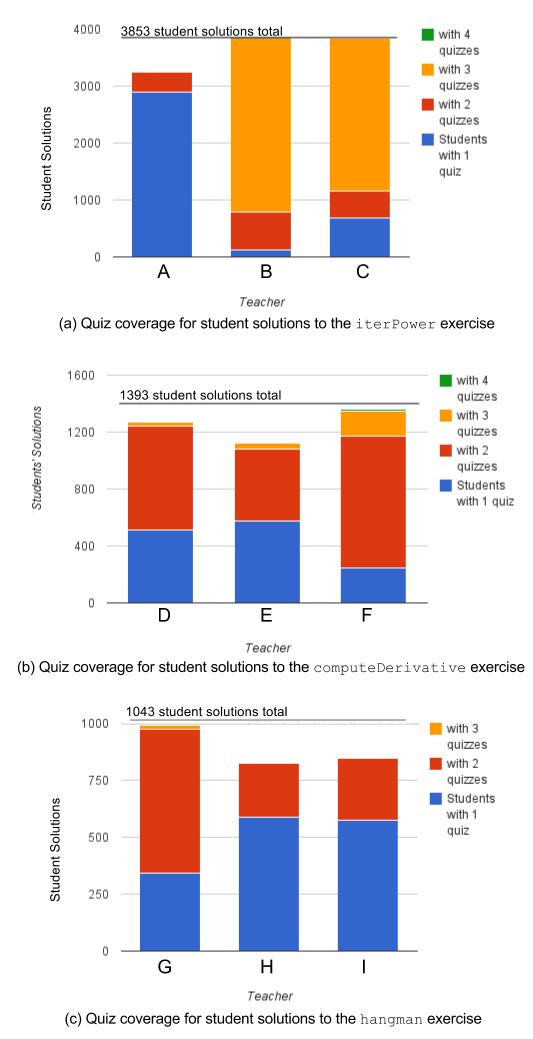
\includegraphics[width=1.0\columnwidth]{Body/figures/foobaz/ComboQuizCoverageFigure2.png}
\caption{Quiz coverage of student solutions across three datasets.}~\label{fig:comboquizcoverage}
%\end{figure}
\end{minipage}

\begin{minipage}{1\columnwidth}
%\begin{figure}
\centering
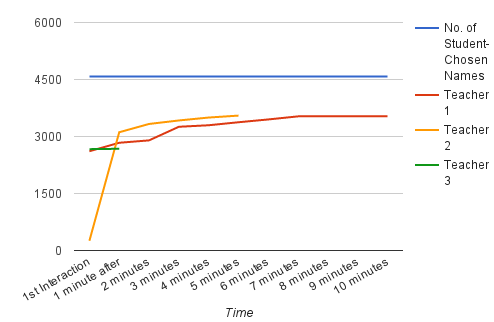
\includegraphics[width=0.9\columnwidth]{Body/figures/foobaz/variableCoverageNoTitle.png}
\caption{Variables in iterPower solutions labeled by each teacher.}~\label{fig:variableCoverage}
\end{minipage}
\end{figure}

\subsection{Student Study}

We ran a second study on the student side of the workflow in order to (1) find out if the teachers' efforts in the previous study produces quizzes that are relevant to these new students and (2) better understand student reactions to this novel form of feedback. In order to do this, we targeted beginner programming students and invited them into the lab to receive personalized quizzes generated by the teachers in our previous study.

Before the start of the study, quizzes composed by teachers using Foobaz in the first user study were rendered using the edX framework, ready to be personalized. Since pilot testing with beginner programming students indicated that six alternative variable names in a quiz is too many, teachers' quizzes were randomly subsampled to include a maximum of five alternative names for students to consider. 

Students came into the lab for one hour and composed solutions to one of the four exercises. After receiving each solution, the experimenter mentally executed the solution and compared the behavior of its variables to the variable behavior covered by the teachers' quizzes. If there was a match to one or more teachers' quizzes, one quiz was randomly selected. The experimenter made a copy of the student's code and replaced every instance of the variable to be quizzed on by an arbitrary symbol, e.g., a bold letter A. The experimenter then appended the quiz to the modified copy of the student's solution and delivered it to the student as a personalized quiz. If there was no match to one or more teachers' quizzes, then the student received a generic quiz, about a variable name in a solution other than their own.

After the student completed their personalized quizzes, they took a survey about their experience. Students who were able to complete the coding exercise and quizzes with significant time left in their session repeated this process for a second programming assignment.

\subsubsection{Apparatus}

In all sessions, we used laptops with 15.4-inch or 13.3-inch screens. All participants' interactions with the system were logged using the edX platform infrastructure.

\subsubsection{Participants}

We recruited 6 participants (4 female) who were either undergraduate or graduate students, through computer science-specific and campus-specific mailing lists, Facebook groups, and word of mouth advertising. Their ages were between 18 and 27 ($\mu=20.4$, $\sigma=3.2$). Four of the participants had taken one or two introductory programming courses on Coursera or at their high school or college campus. The remaining two participants had taken three or four classes that involved learning programming languages or computer science concepts, and had some experience with Python.

\subsubsection{Results}

Six students took a total of 12 quizzes, 11 of which were able to be personalized, even though their solutions were, in some cases, significantly different from the prior student solutions seen by teachers during quiz creation. Correspondingly, in the surveys that followed, students agreed with the statement ``This quiz felt relevant to me'' at an average level of 5.4 ($\sigma = 1.0$) on a 7-point scale. One student's solution did not receive a personalized quiz because its variables behaved in ways that no teacher in the previous study considered. That student was able to understand the new solution and take the quiz, though it had little relation to their own solution.

Students were asked in the post-quiz surveys about what they learned from the exercise. One student replied, ``Possible variable names are pretty much synonyms, but the more detailed/specific ones are better.'' Another wrote, ``It's worthwhile to pick good variable names.'' Students' average level of agreement with the statement ``The quiz made me think about what makes variable names good or bad'' was 6.2 ($\sigma = 0.9$) on a 7-point scale. Mean levels of agreement with statements about the quizzes being confusing or tedious were 2.9 ($\sigma = 1.5$) and 3.4 ($\sigma = 1.2$), respectively, on a 7-point scale.

Some students observed that this was a very subjective quality of their code to be quizzed on, but all students were able to understand and complete the quizzes they were assigned. Some students disagreed with the instructor-provided ratings. When this occurred and the teacher left no explanation, students had at least one of three reactions: (1) They tried to imagine what the teacher was thinking. (2) They expressed displeasure at the lack of explanation. (3) They decided that they still disagreed with the teacher's judgment. Students did pick up on the teachers' preferred naming conventions through the quizzes. As evidence for this, two students correctly wondered aloud whether a different teacher made each of the quizzes they saw during their session. Given the subjectivity of the task, it may be necessary to grade only on participation, rather than absolute agreement with the teacher.

Students were not informed that quizzes were populated largely by fellow student variable names, but one student volunteered their appreciation for a ``wide spectrum'' of variable names to consider. However, randomly sampling teachers' quizzes down to 5 variable names created some student confusion when there were no positive naming examples in the resulting quiz. This is evidence that sampling should be constrained to include both good and bad examples and the user interface should provide some additional guidance to remind teachers that students highly value a balance of examples, each paired with an explanatory comment.

\section{Limitations}

The first study establishes the usability, learnability, and efficacy of
the main Foobaz interface for teachers. The second study is intended to
show that students can understand and use the personalized quizzes that
Foobaz produces. However, this evaluation of the student experience does not yet show pedagogical benefit. To measure learning benefits, we plan to deploy the tool in a
large Python programming course this fall.


\section{Conclusion}

We have designed and studied both the teacher and student sides of a novel interface and workflow for providing feedback on student variable names at scale. We hope it will serve as an example and a design pattern for future work on user interfaces for teaching programming to thousands of students at once.
%\chapter{Statistical Modeling of Solutions}\label{chapter:bayesian}







\section{LDA}


\subsection{Features} 

%Fortunately, programs are also executable. Features from dynamic analysis can complement static token-level features, as was demonstrated in \cite{glassmankimtechreport}. Of particular interest in this work are the features produced by the OverCode program analysis method \cite{glassmantochi}.

%{\bf Common Variables} The OverCode \cite{glassmantochi} analysis pipeline was initially developed to deduplicating Python programs that differ only by variable names, statement order, formatting, and comments. In the process of this deduplication process, 



%\subsection{Model Choice}









%\begin{figure}[ht]
%%\vskip 0.2in
%%\begin{center}
%\includegraphics[width=0.5\columnwidth]{lda_plate_model}
%\caption{Plate model for LDA}
%\label{lda_plate_model}
%%\end{center}
%%\vskip -0.2in
%\end{figure} 



%If we ignored the interdependence of decision choices on each other,  %One can think of this as a tree-structured solution space, where the number of choices that can be made at each decision point

%\section{Feature Choice}

 % rather do not necessarily even stay constant as solution complexity goes up; it may decrease because fewer students are able to compose a correct solution.
%For every additional dimension, one may need many more solutions in order keep the same level of density.





% well suited to summarizing the major design decisions


%Given the relatively small set of underlying design decisions, the common structures shared by many student solutions, and the availability of feature vectors already computed by the OverCode pipeline, appropriately chosen latent variable models may be well suited to summarizing the major design decisions. %and earlier promising experimentation with Bayesian non-parametric methods as part of a collaboration with \citet{beenthesis}, Bayesian non-parametric methods may be key to fulfilling the original vision for OverCode.



%\section{Empirical Qualities of Solution Clusters}





%\section{Model Choice}





\begin{comment}
\section{Plan for Applying Models to Solution Collections}

\begin{enumerate}

\item I implemented a DP-stick-breaking/GEM distribution generator.
\item I studied and understood the stick-breaking construction of the Hierarchical Dirichlet Process found in Section 4.1 of the article Hierarchical Dirichlet Processes by \citet{hdp05}.
\item By April 22nd, I will implement and test, in python, either (1) the Gibbs sampler for CRPs implemented in R and demonstrated in the third MLSS '15 lecture on Bayesian nonparametric statistics or (2) the second algorithm in \citet{neal2000markov}, which performs Gibbs sampling on DPMMs with conjugate priors.
\item By May 4th, I will then generalize the same implementation from the previous step to add a level of hierarchy, in order to perform clustering by Hierarchical Dirichlet Processes. 
\item By May 10th, I will write up the algorithm and its performance on python solutions.
\end{enumerate}

I do have stretch goals, as incentives to finish more quickly, specifically: (1) adding the subspace-learning feature of BCMs to my implementation and (2) predicting rubric labels teaching assistants will apply, based on the labels actually applied by teaching assistants during grading with OverCode.
\end{comment}

%\section{Predicting Rubric Labels}



%\chapter{Learnersourcing Debugging and Design Hints}\label{chapter:classoverflow}

This chapter presents two workflows that prompt students to engage with the diversity of solutions written by fellow students, reflect on their own debugging successes, and write hints that may help current and future students. It is adapted from a paper presented at the ACM conference on
Computer-Supported Cooperative Work and
Social Computing (CSCW) in 2016~\cite{classoverflow}.

One-on-one human tutoring is a costly gold standard in education. As established in Bloom's seminal work on tutoring, mastery-based instruction with corrective feedback can offer a substantial improvement in learning outcomes over conventional classroom teaching \cite{bloom}. However, personalized support does not scale well with the number of students enrolled. In large classes, it is often not feasible for students to get personalized hints from a teacher in a timely manner. Massive open online courses (MOOCs) can have even worse teacher-to-student ratios, by orders of magnitude. Intelligent tutoring systems have strived to simulate the type of personalized support received in one-on-one tutoring, but they are expensive and time-consuming to build. 

The two workflows in this chapter address this problem with a form of {\it learnersourcing}. Prior work on learnersourcing demonstrates that students can collectively generate educational content for future students, such as video outlines and exam questions, while engaging in a meaningful learning experience themselves \cite{kim2013learnersourcing,weir2015,mitros2015}. %The proposed benefit of learnersourcing is that learners are not only more intrinsically motivated to engage with the learning content to begin with, but may also benefit pedagogically from the task itself.

This work builds upon learnersourcing by exploring how it can be applied to the generation of personalized hints during more complex problem solving. While prior work determined which learnersourcing task to present to the student based on what information the {\it system} needed \cite{weir2015}, many educational topics like digital circuit design require some domain expertise that students are not equally well versed in. This raises the question of learnersourcing task routing. More specifically, which learners should be assigned to generate which hints? This work takes on the challenge of generating content that is tailored to both the \textit{hint-receiver}'s current progress and the \textit{hint-author}'s likely level of understanding. 

This chapter presents two workflows for learnersourcing hints that assign hint-generating tasks to students based on what problems the students have recently solved. In the \textit{self-reflection} workflow, students generate hints by reflecting on an obstacle they themselves have recently overcome. In the \textit{comparison} workflow, students compare their own solutions to those of other students, generating a hint as a byproduct of explaining how one might get from one solution to the other. The second workflow can operate on the output of the first, as shown in Figure \ref{fig:workflow}. In both workflows, the key insight is that, through their own experience struggling with a particular problem, students can become experts on the particular optimizations they implement and bugs they resolve. The workflows can take pressure off teaching staff while giving students the valuable educational experiences of reflection and generating explanations. 

While such workflows could have many applications, this chapter describes their deployment in a college-level computer architecture course. In this course, students implement, debug, and optimize simulated processors by constructing digital circuits. During both the debugging and optimization process, hints are one mechanism for teachers to help students fix and optimize their circuits. 

The workflows are applied to two kinds of hints, \textit{debugging hints} and \textit{optimization hints}. A debugging hint is advice written by a student to help a future student change their solution so it generates the expected output for a particular input. An optimization hint is advice written by a student to help a future student get from one correct solution to another, more optimal solution. When hint-receivers encounter that particular situation during their problem-solving process, the hints can be shown to them as if they are the personalized hints an intelligent tutoring system might generate, or that a teacher might provide during a one-on-one interaction. The system for learnersourcing debugging hints is called Dear Beta and the system for learnersourcing optimization hints is called Dear Gamma.

\section{System Design}
There are a number of necessary decisions to make when designing interventions to collect and deliver hints. This chapter provides some answers to key design questions in the context of two systems deployed within a computer architecture class.%: Dear Beta for learnersourcing debugging hints and Dear Gamma for learnersourcing optimization hints.

\subsection{Design Questions} 

{\bf When should students be asked to provide hints?} As soon as a student has resolved a bug, they may have some expertise about that bug that they can share with other students. If too much time has passed between resolving the bug and writing a hint, the student may forget necessary details and context, or forget the bug altogether. A previous learnersourcing system also prompted students to contribute content immediately after having experienced it themselves, for similar reasons~\cite{weir2015}.

{\bf How should students access hints?} Hints can be distributed using either a \textit{push} or \textit{pull} model, and can involve displaying either \textit{all} or \textit{some} of the hints. For example, a push model might display hints as a constantly updating resource, whereas a pull model could dispense hints to individual students just-in-time, when a student requests help. The hints could be algorithmically selected based on the student's work so far and the hints they have already received. This chapter demonstrates both the push and pull models, using the push-all model for distributing debugging hints and the pull-some model for distributing optimization hints. Generating optimization hints was a required reflection activity, so the volume and redundancy of these hints made a push-all model potentially overwhelming.

{\bf What hints can the system designer ask, or allow, a student to generate?} In cases where the student \textit{start state} prior to overcoming an obstacle and \textit{end state} after overcoming the obstacle are known or inferred, the system can ask the student to write a hint that would help someone else overcome the same obstacle. For example, in the case of circuit design, a student who has recently fixed a bug by resolving a particular {\it autograder error} may be capable of writing a debugging hint for other students who get that autograder error. An autograder error occurs when a student solution does not return the expected values. 
%e.g., based on a solution failing one less test case since its last run, e.g., stop failing the same test case

In many cases, however, a student might not face any explicit obstacle, or their start state may not be known. For example, a student might naturally arrive at a highly optimal circuit design without having first tried a less optimal design. Regardless of the path to their solution, the student could generate hints by comparing their own solution to a more optimal solution, or to a less optimal solution. This chapter explores both of these directions by asking each student to do both comparisons. To keep hint generation relevant to the student's current task and to minimize cognitive load, students were not asked to generate hints between pairs of solutions when they were familiar with neither solution.

{\bf How should hints be indexed?} There are many possible ways to index the hints for more accurate retrieval later by students in need. For example, debugging hints could be indexed by the autograder error they are intended to resolve. Optimization hints could be indexed by the student start state, end state, or both with respect to performance. Indexing hints by a meaningful feature of student solutions allows students to more easily find relevant hints in a push model of hint distribution and allows the system to deliver more relevant hints to each student in a pull model of hint distribution. 

The authors made specific indexing choices in order to build Dear Beta and Dear Gamma for students in the computer architecture course. In that course, students run their buggy solutions through teacher-designed sequences of test inputs. Dear Beta indexes debugging hints by the first autograder error that disappears once the bug is resolved. During optimization, the goal is not simply to attain a correct solution, but to arrive at a more optimal correct solution. Dear Gamma indexes optimization hints by both start and end states, which is the leap from a less optimal solution to a more optimal solution that the hint is intended to inspire. These states, the solutions themselves, are complex circuit objects. The number of transistors in a solution as a metric of its optimality. In this indexing scheme, all hints written with the intent of helping a student with a 114-transistor solution create a 96-transistor solution are binned together.

{\bf Which hints should a student receive?} In the push-all model of hint distribution, this question is not relevant, but in the pull-some model of hint distribution, it may be critical. Ideally, students would receive a progression of increasingly specific hints, following patterns of adaptive scaffolding established in intelligent tutoring system literature \cite{andes}, helping them reach a more correct or optimal solution on the spectrum. 

This ideal still leaves room for design choices about exactly which hints to deliver in a pull model of distribution. For example, during the optimization stage of an assignment, the system could \textit{always} give the student hints that help them create the \textit{next optimal solution} found by other students. This would hopefully be an optimization challenge that falls within the student's zone of proximal development \cite{ZMP}. However, this may be too cautious. If a student's solution is far less optimal than the most common solution, then the system could give the student hints to help them leap directly to that most common solution, without first creating any intermediate solutions. This strategy ignores how large a leap outside their zone of proximal development this might be, but it ensures that the student is exposed to the ideas, presented in those hints, that are necessary for implementing a solution at least as optimal as the most common one. Dear Gamma uses this latter option, both hinting students toward the most common solution and hinting students with the most common solution toward the most optimal solution.

{\bf Should hint creation be a required task?} As discussed in Related Work, generating hints can be a valuable part of the learning process. All students were required to generate optimization hints as part of a reflection activity immediately after submitting their first correct circuit. In contrast, writing debugging hints was voluntary. Some bugs, like random typos, do not warrant required reflection.

{\bf How should the variation in hint quality be handled?} 
When it is possible to collect data on helpfulness, collect it. For example, in a user interface, students can upvote hints and hints can be sorted by student upvotes. When hints are being pulled by students in need and there is little or no data about hint quality, the system could deliver multiple hints at a time. Even if one or more hints in the delivered batch are of poor quality, their aggregate message might still be helpful for a student. If most of the hints in the batch are about a feature that is irrelevant to the student receiving the hints, the remaining hint(s) might be about something different and more relevant. Limiting the size of the batch to, for example, five, may prevent students from feeling overwhelmed.

{\bf How public should the hint-author be?} Many systems for question-answering have a reputation system, where the author is known and recognized for contributing answers. Previous work at CSCW has examined whether reputation would improve class forum participation~\cite{reputation}. For simplicity, Dear Beta and Dear Gamma both hide student identities.

\subsection{Self-Reflection Workflow} 

In the self-reflection workflow, students iteratively modify their solutions to pass as many teacher-created tests as possible. For any autograder error revealed by those tests, students can look up hints for what modifications might cause their solution to pass that test case instead. The hints are stored in a database indexed by the autograder errors they are intended to address. When students fix a bug in their own solution, they can reflect on their fix and contribute a hint to the database for others struggling with the same autograder error. The self-reflection step turns a successful bug fix into a shareable hint. It is effectively a self-explanation exercise, since the hint is not a conversation starter. It is meant to stand alone for any future student to consult. As studied in prior work \cite{selfexplanation}, self-explanation helps students integrate new information into existing knowledge.

\subsection{Comparison Workflow} 

In the comparison workflow, students compare their correct solution to alternative correct solutions previously submitted by other students or teachers. They are prompted to compare their solution to a solution \textit{W} with worse performance and generate an optimization hint for students who have solutions like \textit{W}. They are then prompted to compare their solution to a solution \textit{B} with better performance and generate an optimization hint for students who have solutions like their own, which are not yet as performant as solutions like \textit{B}. In each case, the student is generating an optimization hint to help students increase the performance of their solutions. Students who receive these hints use them as guidance while optimizing their own solutions. Figure \ref{fig:workflow} illustrates both workflows.

\begin{figure}
\centering
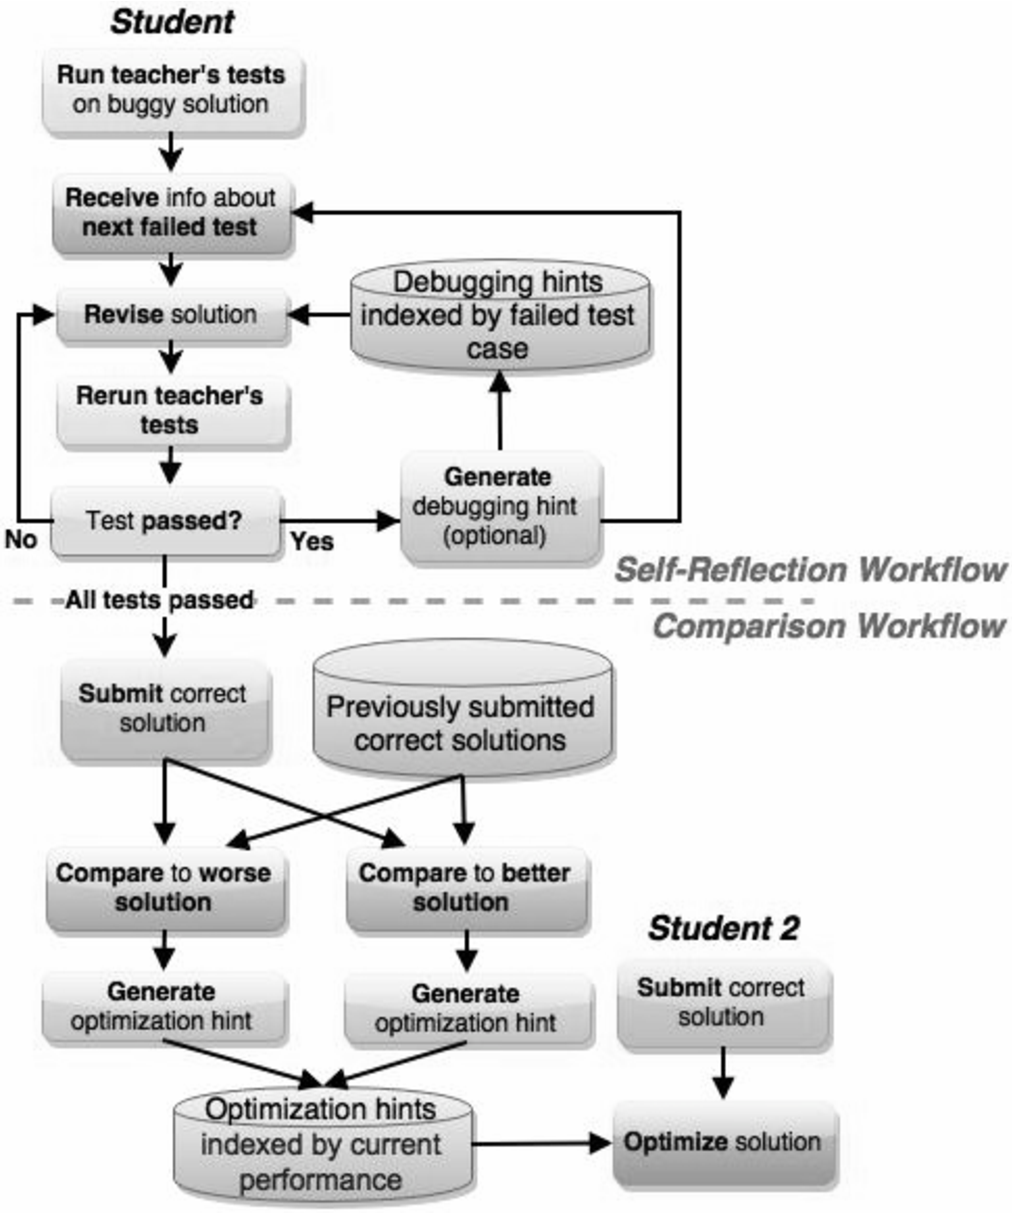
\includegraphics[width=0.75\columnwidth]{Body/figures/classoverflow/CombinedWorkflow_grey.pdf}
\caption{In the \textit{self-reflection} workflow, students generate hints by reflecting on an obstacle they themselves have recently overcome. In the \textit{comparison} workflow, students compare their own solutions to those of other students, generating a hint as a byproduct of explaining how one might get from one solution to the other.}
\label{fig:workflow}
\end{figure}
%\todo{DNHT: Redo this figure}

\section{User Interfaces} 
To learnersource debugging hints with the self-reflection workflow, this chapter presents {\it Dear Beta}, a Meteor web application that serves as a central repository of debugging advice for and by students in the class. The name alludes to both the ``Dear Abby'' advice column and the Beta processor that students create in the class. To learnersource optimization hints with the comparison workflow, this chapter presents {\it Dear Gamma}, a web interface students were required to fill out as a reflection activity after submitting their final correct circuit for a class assignment.
Dear Beta and Dear Gamma each have their own user interface.

\subsection{Dear Beta}

Dear Beta is an application of the self-reflection workflow to processor debugging. Consider students working on their Beta processors within the digital circuit development environment provided by the computer architecture class. Students run a staff-designed test file {\it x} on their circuit. The development environment alerts them to a autograder error: for a particular input (test number {\it n}), {\it y} was the expected output and the student's circuit returned {\it z}. 

Students eliminate autograder errors by fixing bugs in their circuits. They may use trial and error, methodically examine internal simulated voltages, or experience a flash of insight. On the Dear Beta website, they can post a hint for others derived from their insight and indexed by the autograder error it caused. In the process of creating a hint, students have a chance to reflect on their own process of resolving the error.  Other students encountering that autograder error can look up these hints, upvote helpful hints, and contribute new hints. Hints for each error are sorted by the number of upvotes they receive.

After further examining their malfunctioning processor with no success, some students may open the Dear Beta website in order to get help (Figure \ref{fig:hints}). Dear Beta displays all errors and hints, sorted by test file name {\it x}, then test number {\it n}. The student can either scroll to find hints for their autograder error or jump directly to them by entering {\it x} and {\it n} into the bar pinned to the top of the page. If the error was not yet in the Dear Beta system, the error will be added and scrolled into view. 

If there are no hints yet, or if the hints are unhelpful, the student can click the ``Request'' button to the left of the error, which increments a counter. This button helps communicate the need for hints for a particular autograder error to potential hint writers. This is analogous to the ``Want Answers'' button and counter on Quora, a popular question-and-answer site. 

If the student resolves their autograder error and feels that the existing hints were insufficient or incomplete, they can click in the text box labeled ``Add a hint!'' so that it expands into a larger textbox sufficient for typing out a paragraph of their own hint text (Figure \ref{fig:contrib}). Their new hint may be a clearer rephrase of an existing hint or hint at yet another way to resolve the autograder error. Given the variety of processor designs and implementations, there may be several ways any given autograder error may be thrown. 

\begin{figure}
\centering
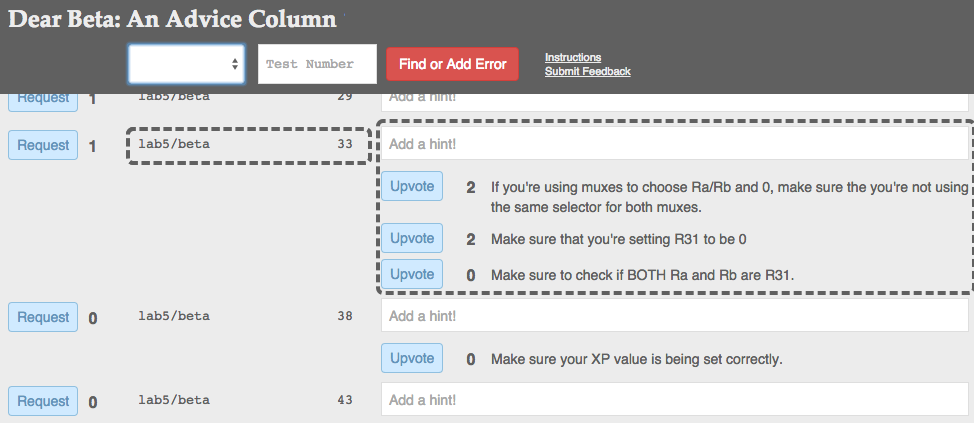
\includegraphics[width=1.0\columnwidth]{Body/figures/classoverflow/hints_modified.png}
\caption{{\it Dear Beta} serves as a central repository of debugging advice for and by students, indexed by autograder errors. In this figure, there are three learnersourced hints, sorted by upvotes, for a autograder error on test 33 in the `lab5/beta' checkoff file.}
\label{fig:hints}

\bigskip
\centering
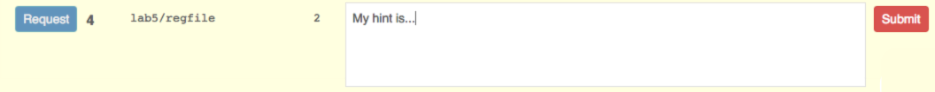
\includegraphics[width=1.0\columnwidth]{Body/figures/classoverflow/contrib_shortened.png}
\caption{After fixing a bug, students can add a hint for others, addressing what mistake prevented their own solution from passing this particular autograder test.}
\label{fig:contrib}
\end{figure}

\subsubsection{Teacher Feedback on Early Prototypes of Dear Beta}

%\todo{finish removing we's}

After deploying initial prototypes of Dear Beta for two semesters, Teaching Assistants were invited to share their complaints, requests, and experiences. Four TAs gave interviews, in person or by email. Their feedback and experiences informed Dear Beta's final design.

Both $TA_{1}$ and $TA_{3}$ adapted to the Dear Beta deployment by first asking each help-seeking student if they had already consulted Dear Beta. If they had not, $TA_{1}$ came back to them after visiting everyone else in the lab help queue. By then, they had often already resolved their problem with Dear Beta hints, and had a new bug they wanted help debugging. 

Dear Beta was used as a debugging aid for both students and teachers. $TA_{2}$ described Dear Beta as a ``starting point'' for students, many of whom used it diligently during debugging. $TA_{2}$ appreciated that students who did ask for her help no longer said, ``My Beta isn't working. Tell me why.'' Instead, they used Dear Beta as a starting point, to help them identify potential locations of a bug in many pages of code. Not just helpful for students, $TA_{3}$ was able to describe with specific examples how Dear Beta \textit{helped him} help students quickly resolve common bugs.

$TA_{2}$ wondered if the extra hints were making it too easy to complete the lab, possibly letting students pass without understanding. $TA_{3}$ echoed this concern, but he made sure each student actually understood the Dear Beta hints whenever he personally guided them through the debugging process.

TAs identified both strengths and weakness in the Dear Beta design. $TA_{1}$ strongly supported Dear Beta's existing design as a single scannable sorted list for quickly finding hints, rather than a purely search-based hint retrieval mechanism or the more general class forum. However, the affordances for contributing new hints in the initial prototype were not obvious and rarely visible on small screens. As a result, $TA_{2}$ was concerned that the level of student involvement in producing hints might be too low. The final Dear Beta design is more externally consistent with other participatory Q\&A systems, has more salient buttons for contributing new hints, and a responsive design that accommodates screens as small as that of a cell phone. 

$TA_{4}$ was absent during most of the Dear Beta deployment but still regularly recommended Dear Beta to students who asked for her help over email. A fifth TA declined to be interviewed. She felt that she had not interacted with Dear Beta enough.

\subsection{Dear Gamma}

To learnersource optimization hints, students participate in the mandatory Dear Gamma hint writing activity right after they first pass all autograder tests for a particular digital circuit, the Full Adder. The student has reached correctness so they are not in a position to think about optimality. %Because students may have arrived at their solution without encountering any particular optimization obstacles, Dear Gamma uses the comparison workflow for learnersourcing rather than the self-reflection workflow. 

\begin{figure}
\centering
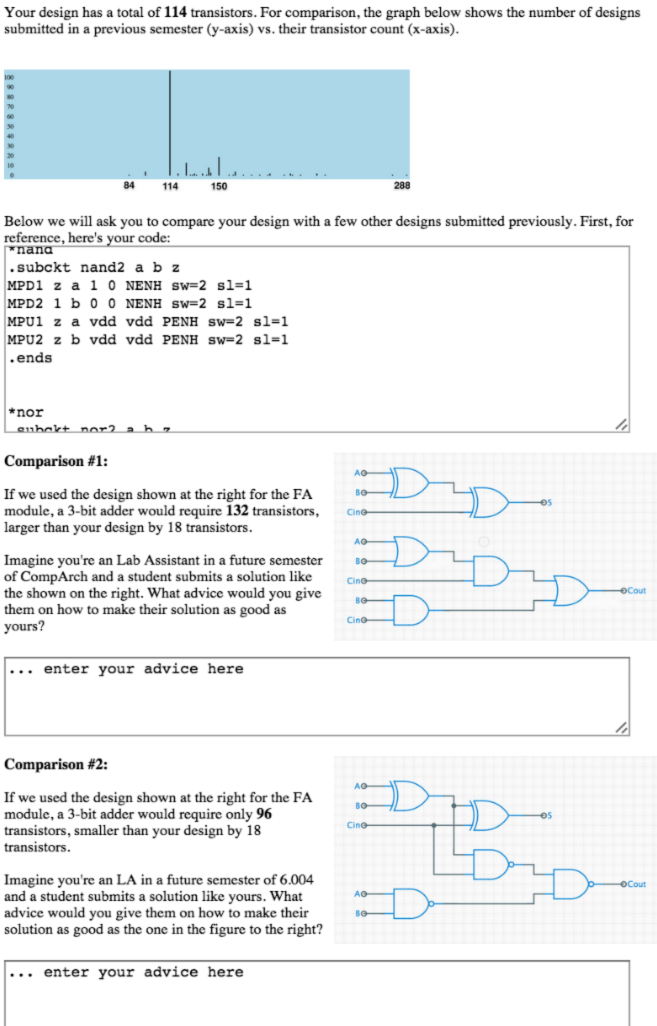
\includegraphics[width=0.70\columnwidth]{Body/figures/classoverflow/deargamma_shortened.png}
\caption{Dear Gamma interface for a student with a solution containing 114 transistors. In the first comparison, they are asked to write a hint for a future student with a larger (less optimal) correct solution. In the second comparison, they are asked to write a hint for a future student with a solution similar to their own so that they may reach the smallest (most optimal) correct solution.}
\label{fig:deargamma}
\end{figure}

To collect Dear Gamma hints, students are given a pair of solutions and asked to give a hint to future students about how to improve from the less optimal solution to the more optimal solution. Students write hints for two such pairs of solutions. In each pair, one of the solutions is always their own. When the student's own solution is the better solution in the pair, then the student can hint at what the author of the less optimal solution might have missed. For example, the student might write, {\it Remember DeMorgan's Law: you could replace the `OR' of `ANDs' with a `NAND' of `NANDs.'} When the student's own solution is the poorer solution in the pair, they are challenged to first understand how the better solution uses fewer transistors, and then write a hint about the insight for a future student who authored a suboptimal solution like their own. 

The comparison workflow was modified slightly, to accommodate the requirements of the course lecturer, who wanted to make sure that all students get a chance to consider both the most common and the most optimal solutions. The collection of previous student solutions in Figure \ref{fig:workflow} was also curated by the lecturer. If a student's solution is larger than the most common solution, they are not shown solutions larger than their own. Instead, they are asked to consider both the most common and the most optimal solutions, so they benefit from seeing both without doing extra work overall. Students with the most optimal solution only consider alternative solutions that are worse than theirs. Figure \ref{fig:deargamma} shows an example of the page for a student with a 114-transistor solution. This was a required activity for all students during one semester of the course and 435 student-written hints were collected from approximately two hundred students who were enrolled in the course. The results of this deployment of the modified workflow is shown in Figure \ref{fig:sankey} as a Sankey diagram of the distribution of solutions connected with student-written hints. %To aid the student in comparing solutions, the Dear Gamma interface displays the student's own solution as a reminder of their design, as well as an alternative picked from among other student solutions.

%Specifically, if a student's solution {\it S} is just as or more optimal than the most common solution, they are asked to (1) write a hint to help a future student with a less optimal solution reach solution {\it S} and (2) write a hint to help a student with solution {\it S} reach the most optimal solution. If a student's solution {\it S} is less optimal than the most common solution, they are asked to write a hint to help a student with solution {\it S} reach (1) the most common solution and (2) the most optimal solution. This scheme ensures that all students are familiar with the most common solution and the most optimal solution and have written two hints to help future students improve the optimality of their solutions. 




\begin{figure}
\centering
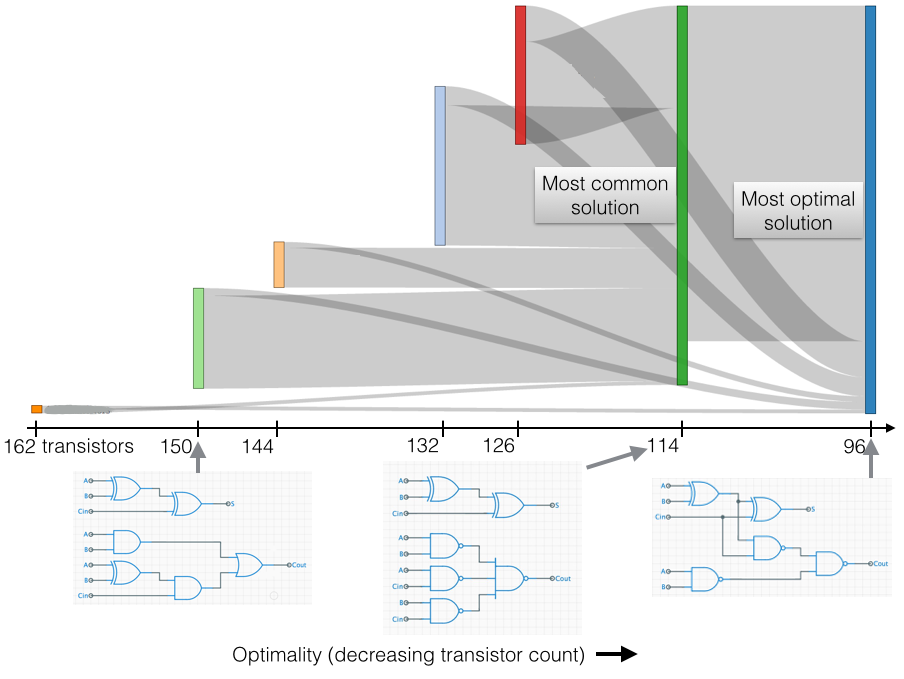
\includegraphics[width=1.0\columnwidth]{Body/figures/classoverflow/annotated_Sankey_onecolumn.png}
\caption{Sankey diagram of hints composed between types of correct solutions, binned by the number of transistors they contain. The optimal solution has only 21 gates and 96 transistors while the most common solution generated by students has 24 gates and 114 transistors.}
\label{fig:sankey}
\end{figure}


\section{Evaluation}

To evaluate the extent to which learnersourced hints can support problem solving, Dear Beta and Dear Gamma were deployed to the computer architecture class, which had an enrollment of more than two hundred students. Dear Beta was deployed for 6 weeks. During that time, the system collected student-generated debugging hints. The Dear Gamma optimization hint collection interface was released to students as a mandatory part of a particular lab. During a later offering of the same course, nine new students were recruited to take part in a lab study designed to shed light on how they solve a typical engineering problem using the learnersourced optimization hints. The questions the evaluation sought to answer are: (1) {\it What are the characteristics of student-generated hints?} and (2) {\it Can students solve problems using those hints?}

\subsection{Dear Beta}
The Dear Beta website was released as a stand-alone additional resource for students one week prior to the due date for the final circuit design lab. Students were made aware of its existence through a class forum announcement and signs on chalkboards in the course computer lab. It was left up for the remainder of the semester for students to refer to, if completing work late. The system tracked student logins and engagement with site features. An initial prototype of Dear Beta was also deployed for two consecutive semesters prior to this final system design and study.

\subsection{Dear Gamma}

\subsubsection{Hint Succession and Categorization}

While Dear Beta makes all hints available at all times, Dear Gamma is modeled on the hint-giving mechanism of an intelligent tutoring system. In prior work, sequences of hints have been posited to facilitate learning due to their similarity with sequences used in expert human tutoring, as well as their support of human memory processes \cite{sottilare2014design}. Therefore, the hints collected with Dear Gamma were decomposed by hand into the three kinds of hints that typically comprise a hint sequence: 1) \textit{pointing hints} direct student attention to the location of error in case the student understood the general principle but did not realize they could apply it there; 2) \textit{teaching hints} explain why a better solution exists by stating the relevant principle or concept; 3) \textit{bottom-out hints} indicate concretely what the student should do \cite{andes}. 

Two researchers independently categorized the 435 collected Dear Gamma hints into six different categories: pure pointing hints ($p$), pointing and teaching hints ($pt$), pure teaching hints ($t$), teaching and bottom-out hints ($tb$), pure bottom-out hints ($b$), and hints that are irrelevant or clearly not helpful. They first independently labeled the first 30 hints. After discussing disagreements and iterating on their understanding of the hint categories, the coders then categorized the remaining 405 hints. 

If one coder labeled a hint as a hybrid between two categories (i.e., teaching and pointing) while the other coder labeled it with only one category (i.e., pointing), the hint was assigned to the pure category (i.e., pointing) that was in common between the two coders' labels. When the categories assigned by each coder did not overlap, the hint was discarded. The minority of hints (3.2\%) labeled as irrelevant or unhelpful were excluded.

\subsubsection{Lab Study}

Nine out of the 226 current students in the computer architecture course participated in the study. These students were recruited through a course forum post and offered \$30 for participating in one hour-long session. The author of this thesis ran all sessions as the experimenter. While obtaining informed consent from each student, the experimenter explained that the study would assess the effectiveness of previously collected hints for optimizing circuits, not the skills of the student. Students were not told that the hints were written by students in a previous semester of the same class specifically for the Adder problem. Instead, the experimenter presented Dear Gamma hints as anonymous, potentially helpful messages. 

Students began the study by reviewing their solution to the Adder problem, which was due earlier in the term. All recruited students had completed it. During the study, three batches of hints were shown in the order of pointing, teaching, and bottom-out, but randomly selected within each category. The experimenter noted the number of transistors in their solution, and randomly selected five pointing-type hints for a solution of that size from the Dear Gamma collection. For example, if the student had 114 transistors in their solution, they received five hints previously generated by students who had written a hint to help improve a 114-transistor solution. Because hints may be of variable quality, the researcher presented hints in batches of five to increase the chances that one of them might be helpful.

The experimenter then asked the student to reduce the number of transistors in their solution. The experimenter explained that there were two more batches of five hints ready for them if they became stuck. These two batches were teaching hints and bottom-out hints. Students could consult outside resources like the course website and Google as well. 

After receiving each batch of hints, participants answered the following 7-point Likert-scale questions about each hint (1: strongly disagree, 7: strongly agree): (1) {\it ``This hint taught me something.''} (2) {\it ``This hint helped me get to a more optimal circuit.''} and (3) {\it ``I feel more confident that I could solve a similar problem in the future.''} These questions were asked immediately after each batch of hints to capture user perception of hints at the time they occurred. However, to avoid slowing down the problem-solving process, participants were asked to explain their answers in writing only after the study, in the post-study questionnaire. This rating process was repeated for the teaching hints and bottom-out hints, even if students were able to solve the problem without asking for these hints.

After the study, users completed a post-study questionnaire regarding their overall impressions. Because users were shown a batch of hints at a time, all of which were student-generated, the post-study questionnaire included additional Likert-scale items, ``I was able to find the most helpful hints and ignore the rest'' and ``Many hints felt repetitive,'' to understand whether users felt they could adequately ignore irrelevant hints. 

\subsection{Limitations}
These studies do not have control groups, so the results cannot support any claims about student learning. Dear Beta was deployed in a real classroom setting while students worked on a relevant class assignment, and the results contain qualitative and quantitative measures of student engagement with the system only. Some of those observed behaviors and opinions may be derived from the participants' sense of novelty, rather than the underlying value of the system. %For the purpose of observing natural interactions with the system, Dear Beta was deployed in a real classroom setting while students worked on a relevant class assignment. 


\section{Results}

\subsection{Dear Beta Study}

For the week prior to the lab assignment due date, the number of registered unique users in the Dear Beta system rose linearly from 20 to 166. It plateaued at 180 by one week after the lab was due. For comparison, the total number of students in the class was 226. 119 students logged in more than once and many students logged in repeatedly.

In the 9 days between the Dear Beta release date and the lab due date, users added 76 autograder errors and 57 hints as a response to those errors. Half of the errors received at least one hint. Seven errors received as many as three hints. Figure \ref{fig:betaengagement} shows user engagement with the system over time. As soon as the initial stock of hints were available, students began upvoting them.

Users contributed 61 upvotes and 10 downvotes on the hints during the same period. The highest number of upvotes (10) was given to the hint {\it ``When entering constants, 1\#4 is 1111 and 1'4 is the 4-bit representation of 1.''} Remember that, while this is a teaching-type hint, it is provided as a targeted troubleshooting hint for students whose solution fails to pass a specific test case. The second most upvoted hint (5 upvotes) was {\it ``Make sure your ASEL logic is correct - don't allow the supervisor bit to be illegally set.''} 

None of the hints appear to be incorrect, though this is difficult to verify, since the teachers do not have copies of the solutions from which these hints were generated. Even within a collection of hints for the same error, not all will be relevant to any particular solution.


\begin{figure}
\centering
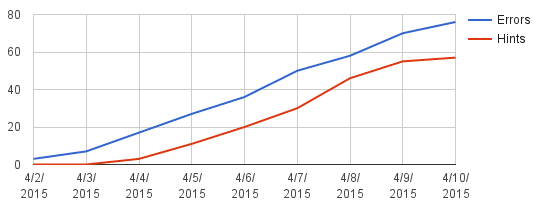
\includegraphics[width=1.0\columnwidth]{Body/figures/classoverflow/cumulativeErrorsAndHints.png}
\caption{Between the Dear Beta release date (4/2) and the lab due date (4/10), autograder errors were consistently being entered into the system. The addition of hints followed close behind.}
\label{fig:betaengagement}
\end{figure}


\subsection{Dear Gamma Study}

With the Dear Gamma hints, six of the nine laboratory subjects were able to improve the optimality of their circuits within the hour that the study took place. Figure \ref{fig:gammaresults} illustrates the subjects' revisions. One student only needed one set of pointing hints. Five students successfully revised their circuits after one set of pointing and one set of teaching hints. Four students received a set of final bottom-out hints as well. Three of those four students ($S_2$, $S_5$, and $S_9$) were still unable to successfully revise their circuits. 

{\bf Hint Distribution} Figure \ref{fig:sankey} is the Sankey diagram of the optimization hints collected by Dear Gamma. The number of hints between certain key transitions, such as between the most common and the most optimal solutions, was far greater because of the lecturer's requests for pedagogically valuable hint prompts that introduced hint-writers to the common and optimal solutions. 

The most common solution size was 114 transistors. Students with that common solution were randomly assigned to generate hints from one of the many different larger solutions down to theirs. These hints are pooled together with the hints written by students with solutions larger than 114 transistors who are seeing the common 114-transistor solution for the first time. Less than five percent of student solutions were the most optimal (96 transistors), but, at the request of the lecturer, every student was asked to consider that most optimal solution and write a hint for a fellow student on how to optimize their solution into that most optimal solution.

Students in the study were drawn from the same population as the hint-generating students, and all study subjects were offered the same number of hints (five pointing hints, followed by five teaching hints, followed by five bottom-out hints) over the course of the hour-long session, regardless of the solution they started with. 

\begin{table*}[t]
\footnotesize
  \begin{center}
    \begin{tabular}{|l|r|r|l|}
\hline
      {\bf Hint type} & {\bf Count} & {\bf (\%)} & {\bf Representative examples} \\
\hline
      Pointing ($p$) & 62 & 14\% & ``You don't have to keep S and Cout as two  \\
       & & & separate/independent CMOS gates.'' \\
      \hline
      Pointing and  & 81 & 19\% & ``Instead of making the S and Cout components individual, \\
teaching ($pt$) & & & combine them together to save computation power.'' \\

\hline
      Teaching ($t$) & 111 & 26\% & ``Instead of recalculating values,  \\
      & & & save computation results to save time!'' \\
\hline
      Teaching and & 19 & 4\% & ``Via application of demorgan's theorem, NAND2 (XOR A B) Cin \\
bottom-out ($tb$) & & & is equivalent to NAND3(NAND2 A B) Cin.''\\
\hline
      Bottom-out ($b$) & 78 & 18\% & ``Use the output of a xor b for one of the nand2 gates.'' \\
\hline
      Unhelpful & 14 & 3\% & ``Use the hints provided by the lab, but try to improve on them.'' \\
      or irrelevant & & & \\
\hline
No coder & 70 & 16\% & \\
agreement & & & \\
\hline
    \end{tabular}
 \caption{Breakdown of Dear Gamma hints by type. Students in the Dear Gamma lab study initially received 5 pointing hints ($p$), followed by 5 pure teaching hints ($t$), and finally 5 pure bottom-out hints ($b$), delivered whenever the student was stuck and asked for more help. }
 \label{tab:hintTypes}
  \end{center}
   
\end{table*}


{\bf Hint Types} Table \ref{tab:hintTypes} shows the breakdown of hints by type, along with representative examples. The Cohen's $\kappa$ \cite{cohen1960coefficient} inter-rater reliability was 0.54, which indicated that the two coders had moderate agreement across the six hint categories \cite{viera2005understanding}. 

{\bf Hint Prompt} Hint-authors interpreted the prompt to create a hint in different ways. Some addressed the hint-receiver directly ({\it ``Keep in mind that...''}), while others addressed the teaching staff ({\it ``I would mention [to the student]...''}). Some hint-authors did not directly write a hint, but instead wrote about how they would approach the situation of being a lab assistant for the hint-receiver: {\it ``I think first I'd ask to make sure they knew what a NAND3 was, because I think a solution like this might come from not totally understanding how it works.''} Still others took a conversational approach, as if they were having an unfolding conversation with the hint-receiver. Interestingly, a number of hint-authors referred to ``here'' or ``my circuit'' in their hints, as if the hint-receiver would be looking at the Dear Gamma interface, with all its examples, rather than just the text generated by the hint-author. This particular assumption on the part of the hint-author was confusing for hint-receivers.

{\bf Optimization Issues} $S_5$ was the only student who had a standard, optimizable solution, received hints, and had no insights about how to optimize the circuit within the allotted hour. $S_1$, $S_2$, and $S_9$'s forward progress was confounded by having near-optimal top-level architecture and very large (suboptimal) implementations of the underlying modules. Dear Gamma only shows hint-authors the top-level architecture, not the underlying gate implementations, for the alternative solutions they compare their own solutions to. They therefore found the hints, which were often about fixing high-level architecture, irrelevant and unhelpful. Even so, $S_1$ was still able to revisit the hints and correctly extract the lesson that only inverting gates should be used. As a result, $S_1$ successfully optimized their circuit.

While using the optimization hints, $S_6$ was the only student who significantly deviated from the correct line of thought by removing all inverting gates. Optimal solutions have only inverting gates. As soon as $S_6$ saw that their transistor count had increased rather than decreased, the student revisited the hints, realized their mistake, and correctly optimized their circuit. None of the hints themselves were incorrect, though some were deemed irrelevant or unhelpful.

{\bf Hint Progression} One student successfully optimized their solution from 150 transistors to the most common solution, 114 transistors, using only pointing and teaching hints. With some time left in the hour-long session, the student opted to optimize their circuit further. The experimenter gave the student one last set of hints, for the transition from 114 to the optimal 96-transistor solution. However, the experimenter did not restart the progression for this next transition. The student was given a set of bottom-out hints instead. Based on these hints, the student got the final optimization step without understanding, and appeared to feel cheated out of the satisfaction of figuring it out himself. 

{\bf Student Reactions} The six subjects without suboptimal gates agreed with the statement {\it ``Overall, these hints helped me get to a more optimal circuit''} ($\mu$=6, $\sigma$=1.1 on a 7-point Likert scale). The remaining three subjects with suboptimal gates disagreed with the same statement ($\mu$=2.6, $\sigma$=2.1 on a 7-point Likert scale). Regardless of whether a subject's solution included suboptimal gates, subjects on average agreed with the statement {\it ``Hints helped me think differently about the problem, even if they didn't directly help me solve the problem'' } ($\mu$=5.4, $\sigma$=1.6).



\begin{figure}
\centering
\includegraphics[width=1.0\columnwidth]{Body/figures/classoverflow/dearGammaResults.png}
\caption{Six of the nine lab study subjects were able to improve the optimality of their circuits with the help of the Dear Gamma hints. Subject S7 was able to make two leaps--one to a common solution with 114 transistors and another from the common solution to the most optimal solution at 96 transistors.}
\label{fig:gammaresults}
\end{figure}

Some subjects commented on the redundancy within each set of five hints of a particular type. This was sometimes expressed as a negative, as in {\it ``These are all hinting at the same thing but I want new information,''} and sometimes expressed as a positive, as in {\it ``Several hints are mentioning X.... I should look into it.''} One student told the experimenter that, while the individual hints were hard to understand, together they formed a clearer picture in her mind about what to do.


\section{Discussion}
In this section, the research questions are revisited first. Then critical design decisions are reviewed, including prompt clarity, index choice for hints, representation choice for alternative solutions, and hint progressions.

\subsection{Answers to Research Questions}

Our study sought to evaluate the characteristics of student-generated hints. Table \ref{tab:hintTypes} shows that students, without coaching, can naturally produce hints that point, teach, give a bottom-out direction, or provide some combination of those elements. However, the number of pointing hints labeled by {\it both} coders as purely pointing-type (22) was much smaller than the number of such hints in the teaching (75) and bottom-out (64) categories. Because students were not informed that their hint would be slotted into a progression, it is possible they may have felt that if they were going to give a future student one hint, it would need to be more substantial than just pointing to a particular location in the solution and hoping the hint-receiver would see the possibility of optimization.

Second, the studies sought to evaluate whether students can solve problems using these hints. Both studies suggest that these student-written hints are helpful. The aggregate activity of students and teachers on Dear Beta indicate that the resource was populated with helpful hints. The Dear Gamma lab study was set up based on the observed sub-optimality of student circuits at the level of choosing and arranging gates. Students whose solutions were suboptimal in that anticipated way rated the hints as helpful. Students whose solutions were suboptimal in unanticipated ways, i.e., at the level of the gates themselves, were not well-served by the hints. Future optimization hint workflows will need both (1) an optimality metric that accounts for multiple common types of suboptimality and (2) a representation of solutions with an appropriate level of detail about the difference between any two solutions. Regardless, the Dear Gamma study suggests that students are helped by the hints when the optimality metric and representation are appropriate.

\subsection{Lessons for Self-Reflection and Comparison Workflows}

Prompt clarity appears to be critical for soliciting the highest possible quality of hints from students. In Dear Gamma, hint collection and delivery were separate processes. Some students misunderstood the prompt and wrote hints as if their audience was still the teacher, not a fellow student. Others did not understand that the hint-receiver would only see the text of their hint, not the diagrams it was based on. In Dear Beta, hint collection and delivery were all mediated through the same, constantly updated interface. The appropriate audience for a hint was clear. Future instantiations of the self-reflection and comparison workflows should clarify who the audience is for hint-authors, perhaps by displaying what students will see. 

The selection of an index for hints in the self-reflection workflow matters. In Dear Beta, the choice of test file name and test number as an index for hints worked well for a class of hundreds of students. In a MOOC-sized course, the index may need to include an indicator that specifies how the test failed as well. Indices in future systems should have sufficient information to group related hints into clusters of a manageable size.

The success of the comparison workflow depends not only on the index for solutions, but also on how these solutions are represented in the workflow prompt for hints. In the comparison workflow, transistor counts did not always capture lower-level reasons for a suboptimal circuit. This resulted in hints that were unhelpful for solutions with lower-level suboptimality. Students will not generate hints that account for what has been abstracted away in the representation of solutions in the hint prompt. Likewise, if the definition of optimality used to index solutions does not account for a certain kind of suboptimality, the hints generated will be unlikely to help future students with that kind of suboptimality. 

Lastly, when students request hints as they did in the Dear Gamma lab study, conforming to the intelligent tutoring system model of providing progressively specific hints is recommended. To automatically create hint progressions in the future, machine learning methods could classify a given hint type. Alternatively, hint type classification could be learnersourced. 

\subsection{Generalization}
Although these workflows were applied to computer architecture problems, the self-reflection and comparison workflows could be extended to other domains. The workflows can be most readily applied to solutions that can be objectively tested for satisfying a set of requirements, e.g., passing unit tests, or whose optimality can be objectively measured. In domains without objective test cases or definitions for optimality, it may be more difficult to establish indices for clustering hints. In these cases, students could be asked to write what challenge they overcame or select from a growing list, enabling others to search for those terms. The comparison workflow could be modified to simply pair students with solutions different than their own, letting them judge for themselves which they think is better, the alternative solution or their own, and write hints based on that judgment.

%\todo{add this: "In the next academic year, we plan to expand our deployment of Dear Beta to two new classes: a MOOC version of the computer architecture class in this paper and a residential college-level software engineering course taken by several hundred students each term. Solutions in the software engineering course are written in Java and tested against teacher-designed test suites. Each error could be specified by the problem set number, test name, and line number. The implementation of Dear Beta has been written generally so that it can simultaneously support both classes, each with their own schema for describing an error."}

\section{Conclusions}
This paper enriches learnersourcing by shaping the design space for learnersourcing personalized hints, and presenting two workflows that engage students in hint creation while reflecting on their own work as well as that of peers. Dear Beta and Dear Gamma are applications of these workflows to the creation of debugging and optimization hints, matching students to the appropriate hint creation task given their current progress. Results from the deployment study and subsequent lab study demonstrate the feasibility of these workflows, and indicate that student-generated hints are helpful to students. They also shed light on critical factors that may impact the quality of learnersourced hints, laying the groundwork for future systems in this area.
%\chapter{Additional Clustering and Visualization}\label{chapter:grovercode}

The original vision of OverCode was to discover pedagogically valuable themes of variation within thousands of student solutions to the same programming problem. While OverCode does normalize and cluster correct solutions so that they can be more easily understood as a group, it does not pull out larger themes of variation as clearly as initially hoped for, nor does it handle incorrect solutions. This chapter describes more recent efforts to address both these shortcomings.

\section{Clustering Solutions with Statistical Models}\label{sec:latent}

One approach to pulling out larger themes of variation within solutions is to cluster more aggressively. The existing OverCode pipeline is a form of deterministic interpretable clustering. What can vary and what is invariant across all the solutions within a cluster is clear, just by reading the platonic solution that represents the cluster. Because it faithfully represents the syntax students used in each cluster, solutions are split apart into smaller clusters by small syntactic differences. 

One promising set of methods for more aggressive groupings of solutions are bottom-up and built on rules. Specifically, these methods define rules for which solutions or groups of solutions can be merged into a single cluster. Probablistic semantic equality or equality with respect to a teacher test suite, which is already used by OverCode for variable names, can be used for subexpressions as well~\cite{}\todo{fill in}. Methods built on program language analysis and synthesis, such as compiler optimizations, could collapse OverCode clusters based on known semantic equality. As a system designer, one must decide or give the teacher control over how many different, semantically equivalent solutions are collapsed into a single cluster since, at the highest level, all correct solutions to the same programming problem are semantically equivalent. These methods are discussed again in the future work, because the second set of methods were chosen for future investigation in this chapter.

The second set of methods leverage statistical properties of the entire corpus of solutions. Given that variation theory is interested in dimensions of variation (and consistency) that characterize all possible instantiations of an idea, statistical methods warrant further investigation. Latent variable models are a type of statistical model that attempt to explain variation in a dataset based on underlying factors. With the right choice of features and model, a latent variable model may be able to capture underlying design choices. In this section, two latent variable models have been explored in a preliminary way for this purpose: the Bayesian Case Model (BCM)~\cite{} and Latent Dirichlet Allocation (LDA)~\cite. 

BCM was selected because, like the original OverCode pipeline, it clusters solutions and produces a single solution to represent the entire cluster. Like OverCode, it also indicates the features that characterize each cluster. While OverCode displays the platonic solution that shares the same set of normalized lines with all other members of the cluster, BCM learns a subspace of features that are most characteristic of the solutions within cluster, in a probabilistic sense. It also has an interactive variant called iBCM, which allows the user to directly modify the prototype and the subspace chosen by BCM if it disagrees with their domain knowledge or preferences. This user modification triggers a rerun of BCM with the modifications taken into account.%is taken into account by the algorithm 

Internally, BCM depends on a mixture model with a Dirichlet prior. Rather than find a cluster for each entire solution, mixture models can learn clusters of features that co-exist across some subset of all solutions. The concentration parameter of the BCM Dirichlet prior is set to promote sparsity, i.e., mixture distributions over solutions that have the majority of their probability mass on a single mixture component. BCM then assigns each solution to a cluster according to its most probable mixture component. %In other words, after fitting the model to the data, each solution will likely have a single dominant mixture component associated with it. If data points were documents instead of solutions, one would say that each document is determined to have a single dominating topic.

LDA was selected as an alternative statistical approach to BCM because of evidence collected at UCBerkeley~\cite{}\todo{fill in} that experts were themselves not particularly consistent about how to cluster solutions. While the LDA output is not as optimized for interpretability as the BCM output, it preserves the ability to examine solutions through the lens of their mixture components, rather than clusters. LDA learns both mixture components, which are distribution over features, and the distributions of those mixtures over each solution in the set it is trained on. Depending on the features chosen to represent solutions, it may be difficult to interpret exactly what a mixture component is just by looking at its distribution over features. However, sorting solutions based on the degree to which a particular topic is associated with them may pull out a distinctive, human-interpretable themes. %Furthermore, when using LDA, the concentration parameter of the Dirichlet prior need not promote for sparsity; it can be tuned by a human or a heuristic, to maximize the usefulness of the resulting breakdown into mixture components. This parameter's optimal value may be problem-specific and teacher-specific. 



\subsection{Interpretable Clustering Solutions with BCM}

BCM was applied to the platonic solutions generated by OverCode. The platonic solutions encode both static and dynamic information in a readable function, i.e., the syntax carries the static information and the variable name encodes dynamic information. The platonic solution is tokenized and represented as binary vectors indicating the existence of the features, including renamed variables and language-specific keywords, such as specific normalized variable names like \texttt{listA} and Python keywords like \texttt{assert} and \texttt{while}. The result is a BCM clustering of OverCode clusters.

In a small pilot study, three introductory Python teachers were each given sets of Python solutions to three different programming problems selected from those previously analyzed in the chapter on OverCode. For each problem, they were asked to create a grading rubric and provide helpful comments for the students, based on interacting with solutions in one of three different interfaces. The three interfaces were: (1) raw solutions in the browser, similar to the control used in the OverCode studies, (2) the OverCode platonic solutions, and (3) a BCM clustering of OverCode clusters, i.e., the prototypes and characteristic features of each BCM cluster, as well as its cluster members. The BCM interface, shown in Figure~\ref{overcode_ibcm}, was running the iBCM variant of the algorithm, so teachers could promote a member of a cluster to be its prototype or click on a token within a prototype--a variable name or keyword--to toggle whether or not it is considered a characteristic feature of that cluster. Both these modifications triggered BCM running in the backend to rerun and send a new clustering to the front end for display. 

Pilot users appreciated the fact that BCM gave some structure to the space of solutions. Rather than a long list of solutions, the interface suggested distinct subpopulations of solutions within the list. However, subjects did not fully understand the probabilistic nature of the clustering method. The presence of a single intruder, i.e., a solution that the teacher believed did not belong in a cluster, caused confusion. This could be ameliorated by giving users more ways to modify the clustering, e.g., allowing users the option to kick an intruder out of a cluster and rerun BCM, or by introducing the tool as a mechanism for discovery instead of organization. Subjects also requested richer or higher-level features than variable names and keywords. Been Kim's PhD thesis~\cite{beenthesis} describes a follow-up full user study comparing the efficacy of BCM vs. iBCM on clustering OverCode cluster-representing solutions.

\begin{figure}[ht]
\includegraphics[width=0.75\columnwidth]{Body/figures/grovercode/overcode_ibcm}
\caption{The solutions on the left are cluster prototypes. The blue solution is the selected cluster whose members are shown in a scrollable list on the right hand side. The tokens contained in red boxes are features that BCM identifies as characteristic of the cluster represented by that prototype. When a user hovers their cursor over a keyword or variable name, e.g., \texttt{len}, it is highlighted in a blue rectangle, indicating that it can be interacted with, i.e., clicked.}
\label{overcode_ibcm}
\end{figure} 

\subsection{Mixture Modeling Solutions with LDA}

As described in the chapter on related work, other researchers have documented a lack of agreement across human-made clusters of student code. One possible explanation for this low consistency across teacher-made clusterings of student code is that solutions are mixtures of design choices and teachers care about different things. As described in~\cite{berkeleymastersthesis}: the clusters can be as straight forward as "1 pt", "2 pts" and "3 pts". If student A writes a solution with a well-written loop and extraneous statements while student B writes a solution with extra loops but otherwise very clean code, teachers can reasonably disagree about which cluster each whole solution should be placed in, depending on whether they believe inefficient control flow or extraneous statements are worse.

Instead of trying to approximate clusterings that humans do not even agree on, it may be more useful to model solutions as mixtures of good and bad design choices. While more sophisticated mixture models' assumptions may ultimately be more appropriate, LDA \cite{lda} as implemented in the Gensim toolbox \cite{gensim} was chosen as the model to evaluate in this preliminary work. 

Like BCM, LDA was run on the platonic solutions. However, the representation of these solutions was also changed: in order to pull out higher-level patterns in approach, rather than lower-level patterns in syntax, solutions were represented solely by the behavior of the variables within them. 

As described in the chapter on OverCode, the OverCode analysis pipeline executes all programs on a common set of test cases and records the sequence of values taken on by each variable in the program. OverCode assumes that variables in different programs that transition through the same sequence of values on the same test cases are in fact fulfilling the same semantic role in the program. %This sequence of values taken on by each variable in each program becomes a signature, i.e., the key to recognizing semantically equivalent variables across programs.  % and can therefore be considered the same {\bf common variable} uniquely defined by that sequence of values.



\begin{figure}[ht]
\includegraphics[width=0.75\columnwidth]{Body/figures/grovercode/recursive_example}
\caption{Example of a recursive student solution.}
\label{recursive_example}
\vspace*{\floatsep}
\includegraphics[width=0.45\columnwidth]{Body/figures/grovercode/whilestandard}
\caption{Example of a student solution using the Python keyword \texttt{while}.}
\label{whilestandard}
\vspace*{\floatsep}
\includegraphics[width=0.5\columnwidth]{Body/figures/grovercode/augmentedwhile}
\caption{Example of a student solution using the Python keyword \texttt{while}, where the student has not modified any input arguments, i.e., better programming style.}
\label{augmentedwhile}
\end{figure} 

Below are the sequences of variable values recorded by OverCode while executing \texttt{iterPower(5,3)} as defined in Figures \ref{recursive_example}, \ref{whilestandard}, and \ref{augmentedwhile}:
\begin{itemize}
  \item {\bf Figure \ref{recursive_example}}
  \begin{itemize}
  \setlength\itemsep{0.05em}
  \item \texttt{exp: 3, 2, 1, 0, 1, 2, 3}
  \item \texttt{base: 5}
  \end{itemize}
  \item {\bf Figure \ref{whilestandard}}
  \begin{itemize}
  \item \texttt{exp: 3, 2, 1, 0}
  \item \texttt{base: 5}
  \item \texttt{result: 1, 5, 25, 125}
  \end{itemize}
  \item {\bf Figure \ref{augmentedwhile}}
  \begin{itemize}
  \item \texttt{exp: 3}
  \item \texttt{base: 5}
  \item \texttt{iter: 3, 2, 1, 0}
  \item \texttt{result: 1, 5, 25, 125}
  \end{itemize}
\end{itemize}

In the previous examples, the input argument \texttt{base} would be considered variable common to all three programs, but the input argument \texttt{exp} would not be. The variable \texttt{result} would also be considered a common variable shared across just the definitions in Figure \ref{whilestandard} and Figure \ref{augmentedwhile}. This allows us to distinguish between programs that calculate the answer in semantically distinct ways, without discriminating between the low-level design decisions about syntax. 

LDA is often applied to corpora of textual documents, where the corpus is represented as a $W \times N$ term-by-document matrix of counts, where $W$ is the vocabulary size across all documents and $N$ is the number of documents. In this representation, the document is represented a bag of word counts, i.e., how many times each word appears in the document. Following this analogy, solutions are represented as a bag of variable behaviors. The matrix representing the solutions in Figures \ref{recursive_example} through \ref{augmentedwhile} executed on \texttt{iterPower(5,3)} is shown in Table \ref{varbydocmat}.

\begin{table}[t]
\caption{Variable-by-Solution Matrix for Programs, where variables are uniquely identified by their sequence of values while run on a set of test case(s)}
\label{varbydocmat}
%\vskip 0.15in
\begin{center}
\begin{small}
\begin{sc}
\begin{tabular}{| l | c | c | c | c | c |}
\hline
%\abovespace\belowspace
Sol- & \texttt{5} & \texttt{1,5,...} & \texttt{3,2,1,0,} & \texttt{3,2,1,0} & \texttt{3} \\
ution& & \texttt{25,125} & \texttt{...1,2,3} & &  \\
\hline
%\abovespace
Fig. \ref{recursive_example} & 1 & 0 & 1 & 0 & 0 \\
Fig. \ref{whilestandard}     & 1 & 1 & 0 & 1 & 0 \\
Fig. \ref{augmentedwhile}    & 1 & 1 & 0 & 1 & 1 \\
\hline
\end{tabular}
\end{sc}
\end{small}
\end{center}
%\vskip -0.1in
\end{table}

Note that, while the entries in Table \ref{varbydocmat} only take on values $0$ or $1$, more complicated definitions may have $n$ instances of, e.g., a variable that takes on the sequence of values \texttt{3,2,1,0}. In that case, there could be an $n$ in the \texttt{3,2,1,0} column for the row corresponding to that solution, or it can be left as a binary indicator. %In other words, true to the assumptions made by LDA, these are occurrence counts, not binary indicators.

%\subsection{Procedure}

In order to run LDA, 3875 student solutions to \texttt{iterPower} were first run on a set of test cases within the OverCode analysis pipeline. The OverCode pipeline produced a set of 977 cluster-representing solutions and a set of features for each solution, including which variable sequences were observed during execution. Another script turned this output into a variable-by-solution matrix for the 977 cluster-representing solutions, which were then fed into LDA for analysis. LDA was run repeatedly with multiple values for the parameter that sets the number of latent mixture components. The results were examined by hand since perplexity and held-out likelihoods are not necessarily good proxies for human interpretability \cite{readingtealeaves}. 

Since the learned mixture components are distributions over variable behaviors, it is easier to inspect solutions which have high amounts of that mixture component within them and infer a theme by comparing them to solutions that contain high amounts of a different mixture component. These comparisons were done by hand for a subset of popular mixture components for each LDA model. One topic comparison captured the difference between solutions like Figure ~\ref{augmentedwhile} and ~\ref{whilestandard}. Another topic comparison exposed the difference between the subpopulation of solutions with extra (unnecessary) conditional statements and the common, more concise solution. In the future, a user interface would be very helpful for this task, especially one which made it easier to compare the output of models with different parameter values. 

LDA applied to a variable-by-solution matrix is a promising method for identifying variation within corpora of solutions to the same programming problem. However, the assumptions made in LDA, such as the independence of mixture components, and requirements, such as explicitly setting the number of mixture components beforehand, may mean that other mixture models, such as the Correlated Topic Model~\cite{}\todo{fill in} or the Hierarchical Dirichlet Process~\cite{}\todo{fill in} will ultimately be a better model fit for this purpose.



\section{Conclusion}
The clustering described in the original OverCode work was relatively limited in scope, but it did produce platonic solutions that can be used for more statistically sophisticated clustering techniques and as a starting point for helping graders understand and grade incorrect student solutions by hand.


%\chapter{Discussion}\label{chapter:discussion}

The systems in this thesis give teachers more awareness about the content generated by students in large programming classes and enable styles of teaching that are usually only feasible in smaller classes, such as discussions of variation and style that are directly driven by what the students have already written. These systems also scale up automated compare-contrast, self-explanation, and formative assessment-style exercises whose content is generated by students and curated by teachers. The current state of the art in theories of how humans learn predict that these supported interactions between teachers and students will enhance learning.
%\todo{DNHT:add citations for value of formative assessment to related work}
\todo{add section about clustering, "OverCode, of course, outliers aren't just annoying or noise -- they could
represent that amazing optimization, or the 10 pages of code instead of
the six lines most other kids generated."}

\section{Design Decisions and Choices}

%As the complexity of code increases, students face more design decisions.

This thesis work began with the vision that a teacher would someday be able to look at a display summarizing hundreds or thousands of student solutions to the same problem and immediately see---and comment on---good and bad design decisions that students made. The number of possible distinct student solutions grows rapidly with the number of design decisions and design choices students can make. 

The solution space could be imagined as an $n$-dimensional space, where each dimension corresponds to a design decision, e.g., whether to solve a problem iteratively or recursively. The design choices students make could be thought of as discrete points along each dimension in that solution space. While the number of distinct combinations of design choices students choose can be large, the number of dimensions in this space, i.e., the underlying design decisions, grows more slowly. 

However, the structure of this hypothetical solution space ignores how design choices affect each other. Some design decisions are mutually exclusive, e.g., looping over a particular array with \texttt{for} or \texttt{while}, some decisions are correlated with one another, and some decisions are completely independent. A tree-like description of the solution space can capture some of these relationships between decisions. If a node represents a design choice, e.g., to loop over an array, there may be two or more choices, e.g., a \texttt{for} or a \texttt{while} loop, that can be represented as child nodes. The choice to use a \texttt{for} loop poses an additional design design, e.g., whether to use \texttt{range} or \texttt{xrange}: \texttt{for i in [x]range(input)}. The average depth of the tree would correspond to the average number of design decisions the students faced and the average branching factor would correspond to the average number of distinct choices students in the corpus make at each decision point.

The curse of dimensionality predicts that, as we add more and more dimensions to the solution space, the density of solutions will decrease and the likelihood that any two solutions occupy the same location in that space will go down. The regularity of code discussed in Related Work should help ameliorate the curse of dimensionality, but only partly. In other domains, it is often necessary to collect more data as the dimensionality of the space increases. However, given that the solutions are generated by students, the number of correct solutions are more likely to go down rather than up as the complexity of solutions, and the associated dimensionality of the solution space, increases.

This vision of the solution space inspired and is shaped by the concrete systems built and described in this thesis. In each system, the dimensions of solution variety have been tamed and orderd by choosing what features to ignore and what features to index by. For example, OverCode ignores white space, comments, variable names, and statement orders. It indexes by normalized lines. In order to assign a variable name quiz, Foobaz looks at the behavior of the variables in the student solution, ignoring everything else about it. Dear Beta and GroverCode forget what values cause a solution to fail a test case, preserving only that the test case has failed. Dear Gamma ignores circuit topology and indexes by the number of transistors.

%It is important to note that this work is not intended to capture an enumeration of all possible design choices and resulting solutions. It is intended to capture the design choices students are actually making. The relative popularity of these choices is discussed in the section that follows.

\section{Capturing the Underlying Distribution}

There will be some design decisions within each solution that are rare and some that are common, some that exemplify good programming practices and others that do not. These decisions might create inefficient solutions, reveal a student's fundamental misunderstanding, or use a feature of the language in a creative way. The distribution of solutions along these dimensions of variation may reflect student prior knowledge, teacher explanations, and common misconceptions. 

Computer scientists are often looking for better ways to find needles in haystacks and computationally-minded social scientists are trying to characterize the haystack~\cite{wallachHaystack}. One could think of Codex~\cite{codex} as a mechanism for finding needles, i.e., particular code fragments, in haystacks, i.e., large collections of open source code. One could also think of Webzeitgeist~\cite{webzeitgeist} as a mechanism for finding needles, i.e., web design choices, in haystacks, i.e., large collections of web pages. OverCode, Foobaz, Dear Beta, Dear Gamma, and GroverCode are trying to faithfully represent the haystack, i.e., the distribution of student solutions and bugs, while also supporting needle-finding.

OverCode characterizes the haystack by identifying and displaying the relative popularity of different correct solutions. It also provides filtering and cluster-merging tools that help teachers find needles, e.g., interesting and unusal solutions. Similarly, GroverCode helps teachers understand the haystack of correct and incorrect solutions by displaying the distribution of solutions as a function of their correctness on test cases.

Foobaz characterizes the haystack of variable naming choices by diplaying the relative popularity of different names in each OverCode stack of solutions and across the entire dataset of solutions. The feature of sorting by popularity allows teachers to see the common names as well as the needles, i.e., uncommon names that might be excellent or terrible. 

The learnersourcing workflows helped students, in addition to teachers, understand the distribution of solutions and bugs. Dear Beta reveals some information about the distribution of failed test cases. The variety of student debugging hints for each failed test case reveals some information about how many different possible problems might cause each failed test case. In Dear Gamma, the optimality of circuit solutions was quantified as the number of transistors. The haystack was characterized by visualizing the distribution of solutions from least to most optimal. This distribution was examined by teachers and given to students after they completed their own solution. The distribution helped teachers identify the most optimal solution, which represented a needle, i.e., a very small proportion of all solutions.

\section{Writing Solutions Well}

The focus on introductory Python programming courses is often just correctness. The MIT EECS introductory Python programming course whose staff used GroverCode makes it a policy not to penalize students on how their solution is written. This means that they sometimes have to hand out full marks to a solution that makes them groan.

This policy may exist for several reasons. The first is the clarity of the policy: if it is correct, it gets full credit. Second is the clarity of the evaluation: if it passes the suite of test cases, it is correct. Third is the apparent appropriateness of the objective for novices: it may be too hard for novices to write a solution well in addition to achieving correctness. % worry about writing well in addition to writing correctly.% bear both the cognitive load of writing a solution well in addition to correctly.

However, it can also be very hard to achieve a correct solution if it is not written well. Something as simple as poor variable names, such as giving an array index a name that suggests it holds the value of the array at that index, can cause students to produce incorrect code.

Just as there is no silver bullet for writing prose well, there is no silver bullet for writing solutions well. Solutions, prose, products, buildings etc., are all designed, and each community has its own ways to help students make good design decisions. For example, in {\it The Sense of Style}, Steven Pinker suggests picking apart examples of good writing to understand what makes them good~\cite{pinkersense}. The software industry uses one-on-one peer review, often called code review, to find bugs and judge design decisions. This may also serve as an informal teaching opportunity for software engineers. Some communities create design studios, where students give and receive constructive criticism from peers. Designed objects are examined individually and also as a group, emulating the conditions for learning from variation espoused by the theories of learning reviewed in the related work. 

Written rubrics can serve as a complement to peer review and design studio practices. For example, some software companies compose and maintain prescriptive style guides against which new code is carefully compared. However, these guides may be more prescriptive than descriptive. In other words, they are not necessarily built on data about how software engineers actually design and write their code. %Code reviews, where peers give feedback on newly written code, are a standard practice in this industry. 

Design studios and peer reviews are not yet a standard practice in programming education. However, peer review practices are now starting to be used in large online courses to make up for small teacher-to-student ratios. Some residential software engineering courses, e.g., MIT's 6.005, also set up infrastructure for peer review. Peer review forces students to engage with some sampling of other student solutions. 

The work in this thesis takes this idea farther. Rather than hope that the randomly assigned peer review experiences provides students with a sufficient variety of examples, the work in this thesis attempts to pull out the design dimensions as well as concrete examples along those dimensions and, when possible, ask students to engage with them in a targeted, personalized way. 

This may be helpful even at the level of introductory programming. For example, according to variation theory, a student will understand the concept of a loop in a more generalized, robust way if they have seen all the different ways in which their peers have written that loop. The teacher can quickly and easily provide an expert perspective by commenting on the popular and rare choices. Students can be overwhelmed by choices. For example, they might ask themselves, {\it Should I use \texttt{range} or \texttt{xrange}? Does it matter?} With concrete examples, teachers can help students identify what matters and what does not. 

%Many students now taking introductory programming courses will take these skills with them to other majors. While computer science majors can acquire the skills of writing code well in more advanced software engineering classes, the lessons in introductory courses on writing code well may be the only ones non-majors ever get.


\section{Clustering and Visualizing Solution Variation}
%The OverCode interface add supervised, interactive component.
The OverCode pipeline performs unsupervised clustering. There are distinct failure modes when using clustering in the context of teachers reviewing solutions. Two are most relevant in this work. First, the representation of the solution and the measure of similiarity between solutions can ignore, hide, or otherwise fail to capture what the teacher cares about. Second, when (1) the teacher cannot easily decide what a cluster means to them based on its members and (2) the clustering algorithm cannot explicitly communicate why the cluster exists, the teacher may not trust the clustering and may not feel comfortable using it for propagating feedback and grades back to students. This is exacerbated when the teacher discovers a member of a cluster that seems not to belong.

The OverCode clustering pipeline attempts to escape the first clustering failure mode: erasing distinctions that the teacher may care about. For reasons discussed in detail in the OverCode chapter, OverCode is designed to reveal to the teacher what their students' solutions actually look like, modulo white space and comments. These solutions are rendered for the teacher using the most common variable names and statement orders.\todo{check the statement order} To stay true to what students actually wrote, this process preserves syntactic differences. For example, when iteratively exponentiating \texttt{base} to an exponent, there are multiple ways to multiply an accummulating variable \texttt{result} by \texttt{base} and save the product back into \texttt{result}, such as \texttt{result *= base} and \texttt{result = result * base}. If the teacher just gave a lecture on common forms of syntactic sugar, OverCode will be sensitive to whether or not students use it. OverCode would allow teachers to observe whether students absorbed the lesson on syntactic sugar based on the way they write their subsequent solutions. The fact that even small differences in syntax creates separate clusters within the OverCode pipeline nearly ensures that any syntactic choices a teacher is interested in has been preserved and can be filtered for in the interface.

 %ignored during the OverCode pipeline %decide for themselves what they want to ignore and 

%\section{Visualization}

The second clustering failure mode---producing clusters that the teacher does not trust---is avoided in several complementary ways. First, there is a clear interpretation of what an OverCode cluster can and cannot include, based on its platonic solution. Specifically, all solutions in the cluster have the same set of lines as the platonic solution after normalizing variable names, standardizing formatting, and removing comments. Second, the differences between clusters is made clear by highlighting which lines make the non-reference clusters different from the reference cluster. Third, the OverCode filtering features and rewrite rules help teachers change their view of solutions into one that preserves the differences they are explicitly interested in and ignores those they are not interested in. Note that filtering by semantic choices may only be possible when the work on Bayesian modeling of these solutions becomes more mature. 

\todo{add "Users do not notice renamed variables unless the names are inappropriate or do not look like they are human generated. Variable names as corpus-wide unique identifiers of a particular variable behavior is externally inconsistent and has low learnability."}

In general, the interfaces in this thesis cluster complex objects and visualize those clusters so that there is little guesswork about what is included and excluded in a group and what the boundary between groups is. There are no outliers that are grouped with something else without explanation. Rather than losing faith in the clustering process, outliers can be used as the teacher sees fit to spur improvements either to the software infrastructure of the course, e.g., the input-output testing harness, or the examples students are asked to engage with. 

\section{Language Agnosticism}

It is not surprising that the evolving values of variables would carry significant semantic meaning in code written by students at the introductory level in languages like Python and Matlab, especially if the style of programming is procedural. This thesis confirms that within the context of introductory procedural Python programs. According to Taherkhani et al.~\cite{taherkhani2010recognizing}, variables carry useful semantic meaning in object-oriented and functional programming styles as well. Gulwani et al.~\cite{gulwani_fse14} and ~\cite{sajaniemi2002empirical} have also authored semantic analyses, i.e., of the C++ and Pascal programming languages, with a focus on variable behavior. OverCode and Foobaz could also be applied to other programming languages. For a language to be displayable in OverCode, one would need (1) a logger of variable values inside tested functions, (2) a variable renamer and (3) a formatting standardization script.

%One could think of it as semantic variable duck typing based on variable behavior. 

%For non-variable-centric languages like Haskell, other dynamic characteristics of execution would likely need to be tracked.

\section{Limitations}

The thesis presents a series of case studies about how to present the variety of programming solutions in a human-interpretable way and make use of it in pedagogically valuable, scalable ways. The methods described only work in a particular domain of solutions: executable programs that solve the same programming problem. This excludes natural language, for example. These case studies embody the design principles espoused, but there is no validated unifying recipe by which a corpus of student solutions can be processed and used. Each corpus and set of teacher values were considered together in order to engineer a representation of solutions--both in the pipeline and in the user interface--that would empower teachers and benefit students. There are many specific technical limitations of the approaches described in the previous chapters. %In the next chapter, the section on future work describes these limitations and suggests next steps.

%I am not aware of any complex domain where this kind of feature engineering and design has been automated. General guidelines and trial-and-error are accepted practice. Before the resurgence of deep neural nets training on massive data sets, one could reasonable argue that carefully human-designed features are were responsible for a great deal of the performance of machine learning systems. Otherwise, systems fall into the failure mode of garbage in, garbage out.

\begin{comment}
\section{Design Recommendations}

While this thesis does not offer a unifying recipe, these are some design recommendations based on experience accumulated since the start of this thesis:
\begin{enumerate}
\item When possible to do with high confidence, propagate human-assigned labels to similar data points.% automatically by the interface, such as grading a single solution and finding out that now an additional 39 solutions will appropriately receive the same grade and feedback.
\item Avoid outliers within clusters at all costs, because they cause doubt and confusion. 
\end{enumerate}
\end{comment}

\chapter{Conclusion}\label{chapter:conclusion}

This thesis demonstrates several ways to capture distributions of student solutions and make this information useful to teachers and students in large programming courses. Capturing commonalities can save teachers time and exhaustion by summarizing many solutions with a single representative. It can also direct teachers to where the majority of the class is within the space of solutions or errors, so they can respond to student needs based on data, not hunches. Capturing variation allows teachers to see how students deviate from the common choices in ways that are superior and deserving celebration or inferior and requiring corrective feedback. These deviations can be used to inspire or directly seed exercises based on modern theories of how students learn generalizeable knowledge from concrete examples. It also saves teachers the time and effort of generating pedagogically valuable examples themselves. Systems in this thesis also demonstrate how the inherent variation in student solutions can be automatically presented back to students, as an active reflection exercise that can benefit both current and future students. 

The technical challenges tackled in order to capture and display distributions of solutions include designing solution representations, measures of similarity between solutions, mechanisms for grouping or filtering them, and human-interpretable displays. Challenges in workflow design centered around simple, minimally-intrusive ways to perform targeted learnersourcing in an on-going programming course.

\section{Summary of Contributions}

The original OverCode system included a novel visualization that shows similarity and variation among thousands of Python solutions, backed by an algorithm that uses the behavior of variables to help cluster Python solutions and generate human-interpretable platonic solutions for each cluster of solutions. The Foobaz system demonstrated how, even when an aspect of variation is hidden in one view of a distribution of solutions, it can be exposed, in context, in a separate view. Additional follow-on work expanded the OverCode normalization process to incorrect solutions and explored additional human-interpretable mechanisms for identifying population-level design alternatives.

Foobaz contributed a workflow for generating personalized active learning exercises, emulating how a teacher might socratically discuss good and bad choices with a student while they review the student's solution together. The Foobaz system demonstrates one concrete way in which a conversation about design decisions, i.e., variable naming, that might only happen in one-on-one interactions with an instructor, can be scaled up to an arbitrarily large class, personalized to each student, be based on the distribution of naming choices found in solutions composed by the teacher's current class or previous classes, and deployed to future classes who assign the same programming problem.

Finally, the self-reflection and comparison workflows demonstrate the potential of targeted learnersourcing. The self-reflection workflow allows students to generate hints for each other by reflecting on an obstacle they themselves have recently overcome while debugging their own solution. The comparison workflow prompts students to generate design hints for each other by comparing their own solutions to alternative designs submitted by other students. Studies of the Dear Beta and Dear Gamma systems show that personalized hints collected through these workflows can be viably learnersourced, and that these hints serve as helpful guides to fellow students encountering the same obstacle or attempting to reach the same goal.

\section{Future Work}
``One never notices what has been done; one can only see what remains to be done...'' - Marie Curie (1984)

There are many directions in which this work can be grown. Some of the research that has been published in parallel with this work can be directly incorporated into future systems. At the same time, many of the existing features can be improved without incorporating any new techniques, based on already collected feedback during user studies, deployments, and other design critiques.

\subsection{OverCode}

OverCode was designed for thousands of correct solutions to introductory Python programming problems. Many residential and online exercises now afford automatic, immediate feedback about the correctness of a solution. Under these conditions, nearly all the final solutions are correct, but it is clear from reading through them that some students have better command of programming than others, just based on compositional quality. As a result, OverCode was designed to reveal to the teacher what their students' solutions actually look like, modulo white space and comments. These solutions are rendered for the teacher using most common variable names and statement orders.%\todo{check the statement order} 

However, as programming problems escalate from the simple to the complex, OverCode's utility breaks down. It can still create platonic solutions and display them in a way that helps teachers spot contrasts, but the clusters themselves become smaller and smaller. As programming problems require more complex solutions, there is also an increasing need to go beyond representing what students actually wrote and toward human-interpretable representations of larger clusters. There are two promising complementary avenues for implementing this next step.

The first avenue is more bottom-up clustering. A critical part of forming OverCode stacks is identifying which variables are semantically equivalent, based on their behavior during execution on the same test cases. Overcode then renames variables to their most common name across all solutions. This normalization process could be extended to subexpressions and code blocks as well, using semantics-preserving transformations, e.g., compiler optimizations, and probablistic semantic equalivalence (PSE)~\cite{codewebs}. OverCode could, in the future, replace semantically equivalent or PSE subexpressions with their most common form across all solutions. Alternatively, this process could be controlled by the user, who decides \DIFdelbegin \DIFdel{the degree to which }\DIFdelend \DIFaddbegin \DIFadd{how much }\DIFaddend they would like to hide less common semantically equivalent subexpressions. An interface like Foobaz could allow teachers to view and compose feedback on the distribution of semantically equivalent subexpressions, just as Foobaz allowed teachers to do for variable names.

%Just as the variation in variable names was hidden by recognizing that variables across programs were semantically equivalent and could be replaced with their most popular student-given name, it may be possible to do the same with respect to semantically-equivalent subexpressions. There two promising ways to determine the semantic equivalence of subexpressions or lines of code in large corpora of student solutions: (1) semantic equivalence based on the rules of the programming language (2) probablistic semantic equivalence based on the dynamic behavior during execution on test cases, as defined in Nguyen et al.~\cite{codewebs}. 

%OverCode could feature an additional button which collapses these detected equivalences, showing the most popular choice in the solution representing the new, larger clusters. An interface, perhaps like the teacher interface in Foobaz, can allow teachers to view and compose feedback that dimension of variation, if they wish. 

The second promising avenue for creating larger clusters is continuing to model the corpus of solutions to the same programming problem as samples from an underlying distribution of solutions shaped by teacher explanations, student prior knowledge, common novice misconceptions, and the constraints of the language itself. Depending on the model chosen, larger clusters could be groups of whole solutions or groups of sub-components the co-occur within many solutions. Iterating on solution representation, model choice, interface, and interaction will hopefully allow teachers to understand their students' design choices, give style feedback, and assign grades with confidence. 

Even simple additions to the OverCode interface could approximate what more sophisticated statistical methods would do. For example, LDA may pull out distributions of commonly co-occuring variable behaviors but the current OverCode interface could be modified to suggest and filter by common sets of strictly co-occurring variable behaviors. This approximation is less robust in the face of noise, but it is at least easier for the teacher to interpret using the language of filtering. %mechanisms. rather than relying on LDA , applied to identify common types of solutions, the OverCode interface could suggest and support filtering for solutions that have a common set of strictly co-occuring variable behaviors. 

When visualizing the resulting clusters, it is important to keep in mind the ease with which teachers can interpret the results. Simple modifications to the OverCode interface can go a long way, such as highlighting the sub-expressions or normalized variable names within lines of code, rather than the entire lines, that separate one cluster from another. Another modification would increase the interpretability of the normalized variables. Since the variable behavior is used to normalize variable names, the values of variables and sub-expressions during execution on a test case could be displayed just beneath or alongside the code, as demonstrated in Kevin Kwok's (unpublished) Python notebook demo, in addition to the way it is currently shown, as a legend mapping each variable name to its behavior beneath a tab that many user study subjects did not consult. 


%\todo{Interface upgrades: talk about beneath-line value annotation like that cool notebook and showing differences at the level of subexpressions, and filtering by sets of common variables in solutions which is like cheap version of lda on variables}

When the program tracing, renaming, or reformatting scripts generate an error while processing a solution, the solution is removed from the pipeline. This percentage of correct edX solutions that did not make it through the pipeline was less than five percent of solutions were excluded from each problem, but that can be reduced further by adding support for handling more special cases and language constructs to these library functions. As solutions get more complex, it will also be necessary to expand the OverCode pipeline to more gracefully handle user-created objects and helper functions. Complementary efforts, like ~\cite{choudhury2016autostyle}, also cannot yet handle more than a single function. This remains a difficult but important hurdle to expanding beyond introductory Python programming courses. As part of this expansion, it may be helpful to adopt the \texttt{observe} construct introduced by Gulwani et al.~\cite{gulwani_fse14} and support teacher annotation of solutions with the observe construct within the OverCode user interface. By soliciting human annotation of important variable values, two variables would not need to behave identically in order to be considered by OverCode as semantically the same.% reduces the need for variables

OverCode could also be integrated with the autograder that tests student solutions for input-output correctness. The execution could be performed once in such a way that it serves both systems, since both OverCode and many autograders require actually executing the code on specified test cases. If integrated into the autograder, teachers could give feedback by writing line- or stack-specific feedback to be sent to students alongside the input-output test results. The OverCode interface may also provide benefit to students, in addition to teaching staff, after students have solved the problem on their own. Cody is a standing example of the value of this kind of design/style feedback. However, the current interface may need to be adjusted for use by non-expert students, instead of teachers. %This would require pipeline and user interface modifications, in order to account for the fact that not all solutions would be returning the same values for each test case.

Simple interface enhancements would give teachers, and potentially students, more freedom to explore. For example, many user study subjects requested the ability to promote any cluster to be the reference cluster. A student might want to see their solution as the reference, at least as a starting point. Similar to the GroverCode sorting mechanism, the OverCode interface could support sorting clusters by their similarity to the reference as well as by cluster size. 

%\todo{add text about boolean variables not being renamable, require more information, perhaps even more than GroverCode collections}

\subsection{GroverCode}

The normalization of incorrect solutions is based on heuristics about co-occurrences of syntax and variable behavior in both correct and incorrect solutions. This was an attempt to see how far the OverCode features could go toward normalizing incorrect solutions in addition to correct solutions, without using any additional technology. 

AutoGrader~\cite{autograder} could also be added to the pipeline. The AutoGrader understands a language for expressing corrections in introductory Python programs. The authors created a list of such possible corrections. If a small subset of those corrections changes a solution's input-output behavior to match a reference solution, Autograder has diagnosed the bug(s) and can automatically correct the solution. It does not take into account which sets of corrections are more common, unlike the design philosophy the defines OverCode. However, the corrections that are applied are guaranteed to convert the incorrect solutions into correct ones. The correct solutions can move through the OverCode pipeline to be normalized and clustered without heuristics. 

If the AutoGrader is added to the pipeline, it will likely move some but not all solutions from the incorrect to the correct category. The corrections that have been automatically applied could be displayed alongside the corrected code in the GroverCode interface, for transparency. The GroverCode process for analyzing and displaying solutions that are still incorrect after being analyzed by the AutoGrader would be unchanged. If the language for expressing corrections is simple and expressive enough that it can be used by graders to write new rules while they are grading, the combined AutoGrader-OverCode pipeline could be rerun to correct any other yet ungraded solutions that are not already automatically corrected. 

A variety of interface updates have been requested by the teachers who used GroverCode during live deployments. For example, some teachers requested the ability to dynamically add new tests to the test suite and to edit student solutions in the interface without switching to an external editor. %These requests have been catalogued and added the the project as feature requests. 

\subsection{Foobaz}

%This is a step on a clear path toward user interfaces that allow teachers to give meaningful feedback to students at scale about a variety of at least partially subjective but important aspects of code. We believe that 
The approach taken in designing Foobaz may be generalizable to other aspects of programming style. Just as OverCode establishes the equivalency of variables based on their behavior during test cases, one could establish the behavior equivalency of larger or more abstract entities, such as student-written lines of code, sets of lines of code, or entire functions. We consider this a class of problems that Foobaz, and similar systems built after it, can tackle. Future iterations of Foobaz-inspired interfaces could also include additional constraints and affordances to encourage teachers to leave more explanations for their assessments, accompanied by better support for reusing common comments. Teachers could also be given the option to augment or overwrite existing labels, e.g., ``too short,'' to match their own preferences. %Finally, based on usage logs and Likert scale ratings on the helpfulness of various features, we will simplify the interface by removing unappreciated features and improve average response times by eliminating redundant computation.

\subsection{Targeted Learnersourcing}

Dear Beta and Dear Gamma were most successful when directly integrated into teachers' existing mandatory assignments or actively promoted by staff. In future classes with supportive teachers, a module can be added to the Dear Beta workflow that \DIFdelbegin \DIFdel{identifyies }\DIFdelend \DIFaddbegin \DIFadd{identifies }\DIFaddend when a student is in a good place to supply a hint and prompts them to do so. This would be an improvement over the current stand-alone website that students are explicitly directed to when they need help, but not when they can give help. Future work on Dear Gamma should include improving the metric for optimality and the rendering of solutions such that all the differences between more and less optimal solutions are visible to reflecting, hint-writing students. One potential future incarnation of the Dear Beta and Dear Gamma workflow is a crowd-sourced intelligent tutor that helps students get to a correct solution and then optimize that solution, completely driven by student-written hints. %To make this happen, the infrastructure to connect these systems to each other and to an existing course needs to be built. 



%\clearpage
%\appendix
%\addcontentsline{toc}{part}{Appendix}

%\chapter{GroverCode Deployment Programming Problems}
\section{Midterm Problems}

\begin{itemize}
\item Question 4: \texttt{power}. Write a recursive function to calculate the exponential \texttt{base} to the power \texttt{exp}.

\includegraphics[scale=0.65]{Body/figures/grovercode/fig_power}

\item Question 5: \texttt{give\_and\_take}. Given a dictionary \texttt{d} and a list \texttt{L}, return a new dictionary that contains the keys of \texttt{d}. Map each key to its value in \texttt{d} plus one if the key is contained in \texttt{L}, and its value in d minus one if the key is not contained in \texttt{L}.

\includegraphics[scale=0.65]{Body/figures/grovercode/fig_give_and_take}

\item Question 6: \texttt{closest\_power}. Given an integer base and a target integer \texttt{num}, find the integer exponent that minimizes the difference between \texttt{num} and \texttt{base} to the power of exponent, choosing the smaller exponent in the case of a tie.

\includegraphics[scale=0.65]{Body/figures/grovercode/fig_closest_power}
\end{itemize}

\section{Final Exam Problems}

\begin{itemize}
\item Question 4: \texttt{deep\_reverse}. Write a function that takes a list of lists of integers \texttt{L}, and reverses \texttt{L} and each element of \texttt{L} in place.

\includegraphics[scale=0.65]{Body/figures/grovercode/fig_deep_reverse}

\item Question 5: \texttt{applyF\_filterG}. Write a function that takes three arguments: a list of integers \texttt{L}, a function \texttt{f} that takes an integer and returns an integer, and a function \texttt{g} that takes an integer and returns a boolean. Remove elements from \texttt{L} such that for each remaining element \texttt{i}, \texttt{f(g(i))} returns \texttt{True}. Return the largest element of the mutated list, or -1 if the list is empty after mutation.

\includegraphics[scale=0.65]{Body/figures/grovercode/fig_applyF_filterG}

\item Question 6: \texttt{MITCampus}. Given the definitions of two classes: \texttt{Location}, which represents a two-dimensional coordinate point, and \texttt{Campus}, which represents a college campus centered at a particular \texttt{Location}, fill in several methods in the \texttt{MITCampus} class, a subclass of \texttt{Campus} that represents a college campus with tents at various \texttt{Locations}.

\includegraphics[scale=0.65]{Body/figures/grovercode/fig_mitcampus}

\item Question 7: \texttt{longest\_run}. Write a function that takes a list of integers \texttt{L}, finds the longest run of either monotonically increasing or monotonically decreasing integers in \texttt{L}, and returns the sum of this run.

\includegraphics[scale=0.65]{Body/figures/grovercode/fig_longest_run}
\end{itemize}
%\import{./Body/appb/}{appb.tex}
%\input{Body/appc}
%\input{Body/biblio.tex}
%%\index{structure!protein|see{protein, structure}}

\clearpage
\printindex

\end{document}

